\documentclass{book}


% Page size
\usepackage[a5paper]{geometry}


% Font
\usepackage{fontspec}
\setmainfont{Clara}
%\setmainfont{IM FELL English PRO}


% Typesetting
\usepackage{microtype}


% Colors
\usepackage[dvipsnames]{xcolor}
\definecolor{darkgray}{gray}{0.35}


% Languages
\usepackage[english, latin]{babel}


% Figures
\usepackage{graphicx}


% Initials
\usepackage{lettrine}


% Columns
\usepackage{paracol}


% Line spacing
\usepackage{setspace}


% Paragraph spacing and indents
\setlength{\parskip}{0.75\baselineskip}
\setlength{\parindent}{0pt}


% Decorative borders
%\usepackage[object=vectorian]{pgfornament}
%\usepackage{tikz}


% Remove page numbers when using cleardoublepage
\usepackage{emptypage}


% Margin notes inside text columns
\usepackage{wrapfig}


% Math
\usepackage{amsmath}


% Put page number at bottom
\pagestyle{plain}


% Counter for english footnotes
\newcounter{engnote}

% Footnotes with their own symbols
\makeatletter
\def\@xfootnote[#1]{%
  \protected@xdef\@thefnmark{#1}%
  \@footnotemark\@footnotetext}
\makeatother

%%%% Note: Footnotes in the english columns should be entered in the latin column using engnotetext, otherwise they may appear on the wrong page.

% Commands for english footnotes
\newcommand{\engnotenum}{\textsuperscript{\arabic{engnote}\stepcounter{engnote}}}
\newcommand{\engnotetext}[1]{\vphantom{\footnotemark{}}\footnotetext{#1}}


% Block headings
\newcommand{\blockhead}[4][]{
\begin{wrapfigure}[#3]{l}{2.75cm}
\centering
\vspace{#4}
\parbox{2.75cm}{\begin{center}\footnotesize \color{BrickRed} \emph{#2}\\ #1 \end{center}}
\end{wrapfigure}
}


\newcommand*\ruleline[2]{\par\noindent\raisebox{.8ex}{\makebox[#2\linewidth]{\hrulefill\hspace{1ex}\raisebox{-.8ex}{#1}\hspace{1ex}\hrulefill}}}


\begin{document}

\pagenumbering{roman}

{\fontsize{11}{11} \selectfont





\begin{titlepage}
\begin{center}


\makebox[\textwidth][s]{

{\fontsize{11}{11} \selectfont \fontspec{IM FELL FLOWERS 2}A}{\fontsize{13}{13} \selectfont \fontspec{IM FELL English PRO}The Chronicle of the Abbey of Bury St.\ Edmunds}

}

\vspace{-0.15cm}

\makebox[.925\textwidth][s]{\fontsize{11}{11} \selectfont \fontspec{IM FELL English PRO}by \emph{Jocelin of Brakelond;} to which are appended several medieval}

\vspace{-0.15cm}

\makebox[.85\textwidth][s]{\fontsize{11}{11} \selectfont \fontspec{IM FELL English PRO}accounts of the life of St.\ Edmund by \emph{Abbo of}}

\vspace{-0.15cm}

\makebox[.775\textwidth][s]{\fontsize{11}{11} \selectfont \fontspec{IM FELL English PRO} \emph{Fleury,} \emph{\AE{}lfric of Eynsham,} and an anonymous}

\vspace{-0.15cm}

\makebox[.7\textwidth][s]{\fontsize{11}{11} \selectfont \fontspec{IM FELL English PRO}author commonly identified with \emph{Robert of}}

\vspace{-0.15cm}

\makebox[.625\textwidth][s]{\fontsize{11}{11} \selectfont \fontspec{IM FELL English PRO}\emph{Gloucester;} here reprinted in their original}

\vspace{-0.15cm}

\makebox[.55\textwidth][s]{\fontsize{11}{11} \selectfont \fontspec{IM FELL English PRO}Latin, Anglo-Saxon, and Middle}

\vspace{-0.15cm}

\makebox[.475\textwidth][s]{\fontsize{11}{11} \selectfont \fontspec{IM FELL English PRO}English with adjacent trans-}

\vspace{-0.15cm}

\makebox[.4\textwidth][s]{\fontsize{11}{11} \selectfont \fontspec{IM FELL English PRO}lations, notes, \& glosses;}

%{\fontsize{20}{20} \selectfont \fontspec{IM FELL FLOWERS 2}d}

%\vfill

%{\fontsize{20}{20} \selectfont \fontspec{IM FELL FLOWERS 2}X}


\vspace{-0.175cm}

{\selectfont \fontspec{IM FELL English PRO}

{\fontsize{8.5}{8.5} \selectfont
\textls[20]{prepared by R.\ Creswell,}
}

\vspace{-0.12cm}


{\fontsize{11.5}{11.5} \selectfont
\textls[350]{\emph{OXFORD:}}
}


\vspace{-0.175cm}

{\fontsize{8}{8} \selectfont
an.do. MMXXI.
}

{\fontsize{12}{8} \selectfont

* \hspace{.4cm} * 

*

}

%{\fontsize{20}{20} \selectfont \fontspec{IM FELL FLOWERS 2}x}

}

\end{center}
\end{titlepage}

\begin{titlepage}
\begin{center}
{\bfseries \lsstyle
{\Large CRONICA}

\vspace{0cm}

{\color{BrickRed} \Huge JOCELINI \\ \vspace*{0.5cm} DE BRAKELONDA,}

\vspace{0.4cm}

{\Large DE REBUS GESTIS SAMSONIS}

\vspace{0.2cm}

{\Large ABBATIS MONASTERII}

\vspace{0.4cm}

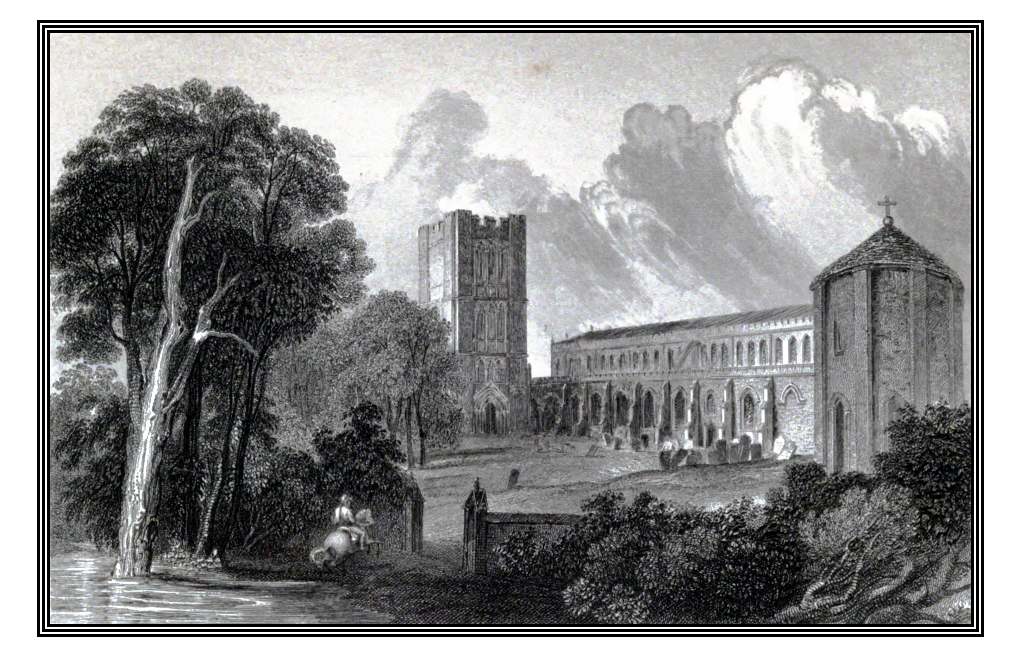
\includegraphics[scale=0.37]{fig/abbey.png}

\vspace{0.4cm}

{\color{BrickRed} \Huge SANCTI \AE{}DMUNDI.}

\vspace{0.2cm}

}
\end{center}
\end{titlepage}


\thispagestyle{empty}
\begin{center}

{\setlength{\parskip}{3mm}

Cronica de rebus gestis Samsonis abbatis

(Harl.\ MS.\ 1005 ff.\ 127r--170v)

Jocelin of Brakelond

}

\end{center}

\vfill

{\setlength{\parskip}{1mm} \small

\emph{Frontispiece---}

G.\ F.\ Sargent and J.\ C.\ Varrall in \emph{The Book of Shakespeare Gems: In a Series of Landscape Illustrations of the Most Interesting Localities of Shakespeare's Dramas}, Bohn, London, \oldstylenums{1846}.

\vspace{0.4cm}

\emph{Latin text---}

Ed.\ T.\ Arnold: \emph{Memorials of St.\ Edmund's Abbey}, Vol.\ \oldstylenums{1}, Rerum Britannicarum Medii \AE{}vi Scriptores, The Lords Commissioners of Her Majesty's Treasury, Under the Direction of the Master of the Rolls, London, \oldstylenums{1890}.


\vspace{0.4cm}

\emph{English translation, introduction and footnotes---}

Trans.\ ed.\ L.\ C.\ Jane, intr.\ Abbot Gasquet: \emph{The Chronicle of Jocelin of Brakelond, Monk of St.\ Edmundsbury: A Picture of Monastic and Social Life in the XII{\tiny TH} Century}, Chatto \& Windus, London, \oldstylenums{1907}.

}


\newpage


\thispagestyle{empty}
\begin{center}

\hspace{0pt}
\vfill

{\setstretch{1.1}

\parbox{5.5cm}{
\makebox[0pt][r]{\emph{``}}{\emph{Fly, noble English, you are bought and sold;\\
Unthread the rude eye of rebellion\\
And welcome home again discarded faith.\\
Seek out King John and fall before his feet;\\
For if the French be lords of this loud day,\\
He means to recompense the pains you take\\
By cutting off your heads: thus hath he sworn\\
And I with him, and many moe with me,\\
Upon the altar at Saint Edmundsbury;\\
Even on that altar, where we swore to you\\
Dear amity and everlasting love.''}
}
}
}

\vfill
\hspace{0pt}

\end{center}


\cleardoublepage

\begin{center}

\hspace{0cm}\vspace{1.0cm}

\parbox{8cm}{

\begin{center}
\textls[100]{EDITORIAL REMARKS.}
\end{center}

\vspace{.25cm}
{\setstretch{1.05}
The paragraphs, headings, and numbered footnotes are those of L.\ C.\ Jane's translation, as it appeared in the \oldstylenums{1907} edition of Chatto \& Windus. Where not completely redundant, T.\ Arnold's (Rolls ed., \oldstylenums{1890}) marginalia and notes have been reproduced as obelus footnotes in the Latin text. Minor printing errors have been corrected throughout. The Fell Types (title page) were digitally reproduced by Igino Marini (\texttt{www.iginomarini.com}).
}
}

\end{center}


\begin{center}

\hspace{0cm}\vspace{1.0cm}

\parbox{8cm}{

\begin{center}
\textls[100]{NOTE CONCERNING CURRENCY.}
\end{center}

\vspace{.25cm}
{\setstretch{1.05}
The \emph{mark} is an archaic northern European weight unit, typically divided into eight \emph{ounces} (of some specification), and used particularly for the measurement of gold and silver. In Norman England it was a unit of account worth \oldstylenums{160} pennies (\oldstylenums{13}s.\ \oldstylenums{4}d. or two-thirds of a pound), \emph{i.e.}, one mark weight of silver, provided that the pennies were not debased. The English pennies of the late twelfth and thirteenth centuries contained approximately \oldstylenums{1}.\hspace{1pt}\oldstylenums{4} grams of fine silver, and were worth about a half day's wage.
}
}

\end{center}


%\cleardoublepage
%\thispagestyle{empty}
%\includegraphics[scale=1,angle=90]{map/export1.pdf}



\cleardoublepage

\begin{center}


\hspace{0cm}\vspace{1.4cm}

\parbox{8cm}{
{\scshape
A veritable monk of Bury St.\ Edmunds is worth attending to, if by chance made visible and audible. Here he is; and in his hand a magical speculum, much gone to rust, indeed, yet in fragments still clear; wherein the marvellous image of his existence does still shadow itself, though f\vphantom iitfully, and as with an intermittent light.\\
}

\hspace{0pt}\hfill Carlyle --- \emph{Past and Present}.
}

\end{center}

\vspace{1cm}

{\setstretch{1.05}

\lettrine[lines=4]{\color{BrickRed}F}{ew} medi\ae{}val documents have exercised a greater fascination over men's minds in these latter days than ``The Chronicle of Jocelin of Brakelond.'' More than sixty years ago the publication of the Latin text of this history, by the Camden Society, attracted the attention of the great Thomas Carlyle, and furnished him with material for sketching his picture of ``The Ancient Monk,'' which occupied the entire second book of his \emph{Past and Present}. Although the modern sage in his own rugged way affected no little contempt for what he called this ``extremely foreign book,'' and for ``the monk-Latin'' in which it was written, it is evident that Jocelin's simple story of the wise, firm, yet withal gentle rule of a medi\ae{}val abbot over a great English monastery cast a spell over him, the influence of which can be detected in every page of his delightful and almost surprisingly sympathetic account of Abbot Samson and of Edmundsbury.

In this case the \emph{Past}, as Carlyle read it in the ``Chronicle,'' was so entirely different from the \emph{Present}, as he knew it in his day, that the wonder is not that he was fascinated by it, but that he was able with its help to paint so true and living a picture and to fashion so fitting a frame in which to set it. For to him, without doubt, the story dealt with what he regarded as ``vanished existences''---``ideas, life-furniture, whole workings and ways,'' which were not only \emph{Past}, but gone beyond recall, and ``covered deeper than Pompeii with the lava-ashes and inarticulate wreck of seven hundred years!''

And indeed it cannot be denied that the ideals and aspirations, as revealed to us in the history of Abbot Samson and, so far as we know, in the life story of his biographer Jocelin, are of a higher and almost a different order to those of our modern world. To men of their calling in those far-off times, the natural and the supernatural were united and intermingled in the simplest and most ordinary way. Their very notions of the unseen world are almost sufficient to take away the breath of those whose lots have been cast in this more material and prosaic age of doubts and disbeliefs. To Samson, and Jocelin, and their fellow-monks at Edmundsbury in the twelfth century, heaven, as a great writer has said of earlier English monasticism, was hardly even ``next door.'' The future life was merely the present continued, and each man went forth to his task as it came and laboured at it day by day, not with any idea of finishing it, but only of carrying on for the span of his allotted existence. They built, and planted, and wrote till the end came, and then they went to heaven and others stepped into their places and took up the common work. It was indeed a ``simple life:'' it was almost Arcadian in its picturesque simplicity, and, as Cardinal Newman says of the same life in the days of our Venerable Bede, it reminds us of those times in the dayspring of the world, when Adam delved and Abel watched the flocks, and Noah tended his vines, and angels visited them.

This living belief in the nearness and all-importance of the supernatural is the key-note of Jocelin's charming story of a few brief years in the long history of an old English abbey, a new translation of which is here given to the public. As a story, however, Brakelond's ``Chronicle'' is not wholly, nor indeed mostly, either mysterious or incredible: there are troubles, and trials, and difficulties enough recounted by the writer; and at every turn we may see evidences of human nature and even of human struggles and passions, which are sufficient, and as some may perhaps think, more than sufficient, to show us that it is a history of men, and not of angels, which the old monk is setting forth so naturally and so truthfully. At any rate, there is quite sufficient of the human element in the narrative to give most of us a human interest in the story.

And this itself is proof that Jocelin is a true chronicler of what really took place, and no mere romancer tempted to edit or suppress entirely what might not be unto ``edification.'' He manifests no desire to make himself or his brethren appear other than what they were in reality---that is, thorough Englishmen, with strong wills and human passions, which, though these same passions might occasionally appear to gain the mastery, they were at all times endeavouring to subdue unto God's service by the help of His grace and through the broad-minded provisions of St.\ Benedict's Rule. The actors who appear in this living drama, though they are for the most part monks, are obviously men, natural and human enough in all their works and words; but these men are at the same time also monks, endeavouring to raise their minds and hearts to supernatural ideals, and striving to attain to that personal communion with God which is the aim and object of all true religion and of all religious observance and practice. This is ``another world truly,'' writes Carlyle, ``and this present poor distressed world might get some profit by looking wisely into it, instead of foolishly. But at lowest, O dilettante friend, let us know always that it \emph{was} a world, and not a void infinite of grey haze with phantasms swimming in it. These old St.\ Edmundsbury walls, I say, were not peopled with phantasms, but with men of flesh and blood, made altogether as we are. Had thou and I then been, who knows but we ourselves had taken refuge from an evil Time and fled to dwell here, and meditate on an Eternity, in such fashion as we could? Alas, how like an old osseous fragment, a broken blackened shinbone of the old dead Ages, this black ruin looks out, not yet covered by the soil; still indicating what a once gigantic Life lies buried there! It is dead now, and dumb; but was alive once and spake. For twenty generations, here was the earthly arena where painful living men worked out their life-wrestle,---looked at by Earth, by Heaven and Hell. Bells tolled to prayers; and men of many humours, various thoughts, chanted Vespers and Matins;---and round the little islet of their life rolled for ever (as round ours still rolls, though we are blind and deaf) the illimitable Ocean, tinting all things with \emph{its} eternal hues and reflexes, making strange prophetic music! How silent now!''

\textbf{The Author.}---Jocelin de Brakelond, the writer of the Chronicle called by his name, was a monk of Edmundsbury. The date of his birth is uncertain, but as he became a novice in that abbey in \oldstylenums{1173}, we may suppose that he was born not later than \oldstylenums{1156}. It has been conjectured that he was a native of Bury St.\ Edmunds, and that his name Brakelond was derived from that of an ancient street of the city, in accordance with the common practice of calling monks by the name of the place from which they came to religion. Little more is known about him than he tells us incidentally in the course of his narrative, but one of his contemporaries in the monastery speaks of him as ``a man of excellent religious observance, as well as a power both in word and work''---\emph{eximiae religionis, potens sermone et opere}. Carlyle sees him in his writing as a man of a ``patient, peaceable, loving, clear-smiling nature.'' A ``wise simplicity,'' he adds, ``is in him; much natural sense; a veracity that goes deeper than words.'' What more can we desire in a writer, especially when we may add that he shows himself to have been a cultured man, acquainted with the ancient authors, quoting Virgil and Horace and Ovid? His knowledge of the Bible is naturally extensive, and, as was common in those days, his very phraseology is obviously founded upon the sacred text. He once likewise cites, with acknowledgment, a short passage from the more modern Ralph de Diceto's \emph{Imagines Historiarum}. Our latter-day philosopher praises him also because he shows himself to have ``a pleasant wit; and to love a timely joke, though in a mild subdued manner; very amiable to see.''

In \textsc{a.d}.\ \oldstylenums{1173}, as just noted, Jocelin entered the community and passed under the care of Samson of Tottington, who subsequently became abbot, but who was then Master of novices. The then abbot, Hugh, was old, and although a high standard of the religious exercises and of the monastic life inside the cloister was maintained, the temporalities were in a sad state, and year by year tended to get from bad to worse, so that Jocelin's early experiences of monastic life were connected with anxieties about the load of debt to money-lenders under which Edmundsbury groaned.

He tells us that he had himself seen bonds for repayment made out to the Jews, under which, for failure to meet the sums falling due, the original loan had grown in eight years from £\oldstylenums{100} to £\oldstylenums{800}. No wonder that the youthful religious questioned his Master of novices as to why some remedy was not found by those in authority for a state of things which meant temporal ruin and disgrace for the community of Edmundsbury.

In \oldstylenums{1180} Abbot Hugh met with an accident and died. After a period of a year and three months the former Master of novices, Samson, then the provident Sacrist, was chosen in his place. It was during this period of vacancy that, in recording something which happened in the monastery, Jocelin incidentally makes mention of another literary work of his own, namely, the \emph{Book of the Miracles of St.\ Robert}, a boy supposed to have been martyred by the Jews in \oldstylenums{1181}, who was entombed in the church at Edmundsbury.

On the election of Samson, Jocelin was appointed his chaplain, and this brought him into the closest connection with the abbot for six years. In \oldstylenums{1198} and \oldstylenums{1200} he was Guest-master, and in \oldstylenums{1212} he held the office of Almoner. In all these offices the future chronicler had exceptional means of acquiring information, and these he utilised in writing the story of Abbot Samson's administration, which is introduced by a vivid sketch of the temporal disorder of the house in the closing years of Abbot Hugh. His Chronicle covers the period of the history of Edmundsbury from \oldstylenums{1173} to \oldstylenums{1190}, and, as he says in the beginning, ``he took care to write only what he himself saw and heard.'' The date of his death is uncertain.

\textbf{The ``Chronicle.''}---The Latin text of \emph{Cronica Joceline} is found complete only in one manuscript---Harl.\ MS.\ \oldstylenums{1005}---in the British Museum. It was printed for the first time by the Camden Society in \oldstylenums{1840} under the editorship of I.\ G.\ Gage Rokewood, who supplied a valuable Introduction and notes, of which subsequent editors have availed themselves. The text was likewise printed in Mr.\ Thomas Arnold's \emph{Memorials of St. Edmund's Abbey} (Rolls Series) I., pp. \oldstylenums{209}--\oldstylenums{336}.

In \oldstylenums{1844}, under the title \emph{Monastic and Social Life in the Twelfth Century, as exemplified in the Chronicle of Jocelin of Brakelond, A.D. \oldstylenums{1173}--\oldstylenums{1202}}, the work was translated by Thomas Edlyne Tomlins. Carlyle's work, \emph{Past and Present}, published in \oldstylenums{1843} had already drawn attention to the ``Chronicle of Jocelin,'' and another edition of Mr. Tomlins' work was called for in \oldstylenums{1849}. This translation has since appeared at least once, but for the present edition a new English version has been carefully prepared from the original Latin text of the Chronicle.

\textbf{Abbot Samson.}---The central figure and, as we may say, ``the hero'' of Jocelin's story is, of course, Abbot Samson. He was born in \oldstylenums{1135} at Tottington, near Thetford, in Norfolk. His father appears to have died when Samson was young, and a pretty legend of a boyish dream in which St.\ Edmund extended his protection to the child against the assaults of the devil, and the recognition of the place seen in the dream as the gate of the monastery of St.\ Edmundsbury, when his mother had taken him with her on a pilgrimage to the shrine of the saint, led to his taking refuge in the cloister. He had received his early instruction from a schoolmaster named William of Diss, and he attained the degree of Master of Arts in the University of Paris. In this place we are not concerned with the events of his life: these may be read for the most part in the Chronicle of Jocelin of Brakelond. What alone seems to be called for in this brief Introduction is some account of his person and character as it is manifested in the scattered evidences of his acts.

If we want a picture of the man let us take Carlyle's, who sketches ``the substantial figure of a man with eminent nose, bushy brows, and clear-flashing eyes, his russet beard growing daily greyer,'' and his hair which, before his elevation to the abbot's chair, had been black, becoming daily more and more silvered with his many cares. We know something of the task that was before him when he gathered up the reins of office, and we may be sure he knew more. But as we see him in the pages of Jocelin, he was not the man to flinch from his duty, or to seek to let difficulties mend themselves by pretending that he did not see them. From the time that he walked barefooted into his church to be installed in the abbatial chair, he let all see that he was abbot and had come to rule. He had set his whole strength to accomplish a great task and his shoulders to sustain an almost overwhelming burden, when in the hour of his election he walked to the altar singing the \emph{Miserere mei} with his brethren. ``His head was held erect,'' says the faithful Jocelin, ``and his face showed no change,'' a portent which called from the king the remark: ``This abbot-elect seems to think himself capable of governing an abbey.''

``It is beautiful''---writes Carlyle in a philosophical appreciation of the principles of monastic government---``it is beautiful how the chrysalis governing-soul, shaking off its dusty slough and prison, starts forth winged, a true royal soul! Our new abbot has a right honest, unconscious feeling, without insolence as without fear or flutter, of what he is and what others are. A courage to quell the proudest, an honest pity to encourage the humblest. Withal there is a noble reticence in this Lord Abbot: much vain unreason he hears; lays up without response. He is not there to expect reason and nobleness of others, he is there to give them of his own reason and nobleness. Is he not their servant, who can suffer from them and for them; bear the burden their poor spindle-limbs totter and stagger under; and in virtue of \emph{being} their servant, govern them, lead them out of weakness to strength, out of defeat into victory?''

Abbot Samson ruled over his house for thirty years, and when in \oldstylenums{1212}, ten years after the end of Jocelin's Chronicle, he died, he was followed to the grave by a sorrowing community whose unstinted reverence and affection he had won. An unknown monk of Edmundsbury, the author of another Chronicle of the house, thus wrote of him: ``On the \oldstylenums{30}th December, at St.\ Edmund's, died Samson, of pious memory, the venerable abbot of that place; after he had prosperously ruled the abbey committed to him for thirty years and had freed it from a load of debt, had enriched it with privileges, liberties, possessions and spacious buildings and had restored the worship of the church both internally and externally, in the most ample manner. Then bidding his last farewell to his sons, by whom the blessed man deserved to be blest for evermore, whilst they were all standing by and gazing with awe at a death which was a cause for admiration, not for regret, in the fourth year of the interdict he rested in peace."

The first business to which Abbot Samson applied himself after his election was the task of understanding and grappling with the deplorable financial state of his house. He insisted upon the immediate production of every claim against the monastery, and by personally visiting each of its many manors he gained a correct knowledge of its resources. Within twelve months he had formed his plans and had quieted every creditor: within twelve years the entire debt had been paid off, and he could turn his attention to building and adorning the house of St.\ Edmund. It is impossible to read the pages of Jocelin without seeing that the ruling idea of the abbot's life was his devotion to his great patron, St.\ Edmund. He was the servant, after God, of the saint, his representative and the upholder of his honour and privileges, the champion of his rights, the guardian of his property. Inspired by this thought he worked to make Edmundsbury worthy of its patron, and in his success he saw the result of the saint's intercession and protection.

``Apart from this special devotion to St.\ Edmund, it is easy to see,'' writes Mr.\ Thomas Arnold, ``that Samson was an earnestly religious man, and not a Christian by halves. After the news had come of the capture of Jerusalem by the Saracens, Samson took the loss of the Holy Places so much to heart, that from that time he wore undergarments of hair-cloth and abstained from the use of meat.''

He was, too, a thorough Englishman, and read admirably---\emph{elegantissime}---the Bible in English---\emph{scripturam anglice scriptam}---and ``he was wont to preach to the people in English---but in the dialect of Norfolk where he had been born and bred.'' On one occasion he gives as a reason, and as some may think, a somewhat strange reason, for appointing a monk to an office, that ``he did not know French.'' He was no doubt anxious to secure that St.\ Edmundsbury should be truly national, with its roots deep in the soil of his country, to teach it to build up its own traditions, and to let people see that it was a great \emph{English} house.

But Samson's work was not accomplished without grave anxiety, none the less because it was unseen by others. Though he walked upright with a smiling face, and had ever the courage to battle for the rights of his house when there was need, in a way that might make people regard him as a man of iron nerve possessed of a soul that never felt any trouble, nevertheless in the first fourteen years of his administration his black hair was blanched as white as snow, and Jocelin speaks of hearing his beloved master walking about when all were in bed and relieving his pent-up feelings with sighs and groans. Once the chronicler took courage to tell his master that he had thus heard him in his night vigil, and to this the abbot replied: ``'Tis no wonder: you (as my chaplain) share in the streets of my office, in the meat and drink, in the journeys and the like, but you little think what I have to do to provide for my house and family, or of the many and difficult matters of my pastoral office, which are always pressing upon me: these are the things which make my soul anxious and cause me to sigh.''

And so when Abbot Samson came to die, the thin veil which to him and his monks of Edmundsbury alone hid the world to come from their vision was parted, and the supernatural life eternal was revealed to him in the most natural of ways. He passed from labour for God and St.\ Edmundsbury, to rest in God and with his loved patron, carrying with him the full sheaves of his good works. Carlyle has only partially caught the idea when he writes: ``Genuine work alone, what thou workest faithfully, that is eternal.'' ``Yes,'' he concludes, ``a noble Abbot Samson resigns himself to oblivion; feels it no hardship, but a comfort; counts it as a still resting-place, for much sick fret, and fever, and stupidity, which in the night-watches often made his strong heart sigh.''
}
}


\begin{flushright}
\parbox{6cm}{
\begin{center}
\textsc{Francis Aidan Gasquet},\\
\vspace{0.1cm}
\emph{Abbot-President of the English Benedictines}.
\end{center}
}
\end{flushright}

\cleardoublepage
\footnotelayout{m}
\emergencystretch 1em
\pagenumbering{arabic}




\begin{paracol}{2}

\lettrine[lines=4]{\color{BrickRed}Q}{uod} \begin{otherlanguage}{latin}vidi et audivi scribere curavi, qu\ae{}dam mala interserens ad cautelam, qu\ae{}dam bona ad usum,\linebreak qu\ae{}~\hspace{1.6cm}contigerunt in ecclesia sancti \AE{}dmundi in diebus nostris, ab anno quo Flandrenses capti sunt extra villam, quo habitum religionis suscepi, quo anno Hugo prior depositus est, et R.\ prior substitutus.
\end{otherlanguage}

\switchcolumn

\lettrine[lines=4]{\color{BrickRed}I}{ have} undertaken to write of those things which I have seen and heard, and which have occurred in the church of Saint Edmund, from the year in which the Flemings were taken\footnote{The allusion is to the battle of Fornham, November, \oldstylenums{1173}. In this year the quarrel between Henry II. and his sons, culminated in a general rising both in Normandy and in England. Of the leaders of the rebellion in England, Robert de Bellemont, earl of Leicester, was the chief. Having gathered a force of mercenaries in the Low Countries, he landed at Walton, which he failed to take. After joining hands with Hugh Bigod, earl of Norfolk, at Framingham, and capturing Haughley, he attempted to force his way to his own estates. Meanwhile, the justiciar Richard de Lucy and Humphrey Bohun hastened south from their campaign against the Scots, and having been reinforced by the local levies, they succeeded in intercepting Leicester at Fornham St.\ Geneveve, on the river Lark, four miles south from Bury St.\ Edmund's. The rebels were easily defeated, and Leicester taken prisoner; of his mercenaries only a few escaped. An account of the battle, not very accurate, from the point of view of the St.\ Edmund's monks, is to be found in Appendix E of the first volume of the \emph{Memorials of St.\ Edmund's Abbey}, (Rolls Series). The escape of those mercenaries who did escape is attributed to the intervention of St.\ Edmund and St.\ Thomas.} without the town, in which year also I assumed the religious habit, and in which Prior Hugh was deposed and Robert made Prior in his room. And I have related the evil as a warning, and the good for an example.

%\switchcolumn*

\end{paracol}
\begin{paracol}{2}

\begin{otherlanguage}{latin}
\blockhead[\textsc{a.d}.\ \oldstylenums{1173}.]{How Abbot Hugh ruled the Church of St.\ Edmund.}{4}{-0.45cm}
Tunc temporis senuit Hugo abbas, et aliquantulum caligaverunt oculi ejus; homo pius et benignus, monachus religiosus et bonus, sed nec bonus nec providus in s\ae{}cularibus exercitiis: qui nimis confidebat suis et nimis eis credebat, de alieno potius quam de proprio pendens consilio. Ordo quidem et religio fervebant in claustro, et ea qu\ae{} ad ordinem spectant; sed exteriora male tractabantur, dum quisque, serviens sub domino simplice et jam senescente, fecit quod voluit, non quod decuit. Dabantur vill\ae{} abbatis et omnes hundredi ad firmam; nemora destruebantur; domus maneriorum minabantur ruinam; omnia de die in diem in deteriorem statum vertebantur. Unicum erat refugium et consolationis remedium abbati, denarios appruntare; ut saltem sic honorem domus su\ae{} posset sustentare. Non erat terminus Pasch\ae{} nec sancti Michaelis octo annis ante obitum ejus, quin centum libr\ae{} vel ducent\ae{} ad minus crescerent in debitum; semper renovabantur cart\ae{}, et usura qu\ae{} excrevit vertebatur in katallum.

\end{otherlanguage}

\switchcolumn

In those days Abbot Hugh\footnote{Hugh, prior of Westminster, was elected abbot in \oldstylenums{1157}, in succession to abbot Ording. According to Gervase (I., 163), he received his benediction from Theobald, archbishop of Canterbury, to whom he made profession of canonical obedience. According to the \emph{Chronica Buriensis} (\emph{Mem}.\ III., \oldstylenums{6}) he was confirmed by the bishop of Winchester. In any case, abbot Hugh, as it related in the text of the \emph{Chronicle of Jocelin} (p.\ \oldstylenums{6}), was freed from all obedience by pope Alexander III.} grew old, and his eyes were dim.\footnote{Gen.\ xxvii., \oldstylenums{1}.} He was a good and kindly man, a godfearing and pious monk, but in temporal matters he was unskilful and improvident. He relied too much on his own intimates and believed too readily in them, rather trusting to a stranger's advice than using his own judgment. It is true that discipline and the service of God, and all that pertained to the rule, flourished greatly within the cloister, but without the walls all-things were mismanaged. For every man, seeing that he served a simple and ageing lord, did not that which was right, but that which was pleasing in his own eyes. The townships and all the hundreds of the abbot were given to firm; the woods were destroyed, and the houses on the manors were on the verge of ruin; from day to day all things grew worse. The abbot's sole resource and means of relief was in borrowing money, that so it might at least be possible to maintain the dignity of his house. For eight years before his death, there was never an Easter or Michaelmas which did not see at least one or two hundred pounds added to the debt. The bonds were ever renewed, and the growing interest was converted into principal.

\switchcolumn*

\begin{otherlanguage}{latin}
Descendebat h\ae{}c infirmitas a capite in membra, a pr\ae{}lato in subjectos. Unde contigit quod quilibet obedientiarius haberet sigillum proprium, et debito se obligaret tam Judeis quam Christianis pro voluntate sua. S\ae{}pe capp\ae{} seric\ae{}, et ampull\ae{} aure\ae{}, et alia ornamenta ecclesi\ae{} impignorabantur, inconsulto conventu. Vidi cartam fieri Willelmo filio Isabel mille librarum et xl.; sed nec causam nec originem scivi. Vidi et aliam cartam fieri Isaac, filio Raby Joce, cccc.\ librarum, sed nescio quare. Vidi et tertiam cartam fieri Benedicto Judeo de Norwico, octies c.\ librarum et quater viginti; et h\ae{}c fuit origo et causa hujus debiti.
\end{otherlanguage}

\switchcolumn

This disease spread from the head to the members, from the ruler to his subjects. So it came to pass that if any official had a seal of his own, he also bound himself in debt as he listed, both to Jews and Christians. Silken caps, and golden vessels, and the other ornaments of the church, were often placed in pledge\footnote{This was illegal. Rokewode (\emph{Chron.\ Joc}., pp.\ \oldstylenums{106}--\oldstylenums{7}) gives instances of fines inflicted on Jews for taking church property in pawn, from the Pipe Rolls of Norfolk and Suffolk.} without the assent of the monastery. I have seen a bond made to William Fitzlsabel for a thousand and two score pounds, but know not the why nor wherefore. And I have seen another bond to Isaac, son of Rabbi Joce, for four hundred pounds, but know not wherefore it was made. I have seen also a third bond to Benedict, the Jew of Norwich, for eight hundred and fourscore pounds, and this was the origin and cause of that debt.

\switchcolumn*

\begin{otherlanguage}{latin}
Destructa fuit camera nostra, et recepit eam Willelmus\engnotetext{William Wardell (\emph{Mem}.\ II., \oldstylenums{291}). His incompetence is mentioned in the \emph{Gesta Sacristurum (ibid.)}, and is described in the text.} sacrista volens vel nolens, ut eam instauraret; et occulte appruntavit a Benedicto Judeo xl.\ marcas ad usuram, et ei fecit cartam signatam quodam sigillo quod solebat pendere ad feretrum sancti \AE{}dmundi, unde gild\ae{} et fraternationes solebant sigillari, quod postea sed tarde fractum est, jubente conventu. Cum autem crevisset debitum illud usque ad c.\ libras, venit Judeus portans literas domini regis\engnotetext{The Jews were legally the king's chattels, and debts due to them were due to the king. Accordingly, when debtors failed to pay, the Jews were able to invoke the royal authority to enforce payment.} de debito sacrist\ae{}; et tunc demum patuit quod latuit abbatem et conventum. Iratus autem abbas voluit deponere sacristam, pr\ae{}tendens privilegium domini pap\ae{}, ut posset deponere Willelmum sacristam suum, quando vellet. Venit autem aliquis ad abbatem, et, loquens pro sacrista, ita circumvenit abbatem, quod passus est cartam fieri Benedicto Judeo cccc.\ librarum, reddendarum in fine iiij$^\text{or}$ annorum, scilicet pro c.\ libris qu\ae{} jam excreverant in usuram, et aliis c.\ libris quas idem Judeus commodavit sacrist\ae{} ad opus abbatis. Et sacrista suscepit omne debitum illud reddendum in pleno capitulo, et facta est carta sigillo conventus signata, abbate dissimulante et sigillum suum non apponente, tanquam illud debitum non pertineret ad illum. In fine vero quatuor annorum non erat unde illud debitum posset reddi; et facta est nova carta octies c.\ librarum et quater viginti librarum, reddendarum ad terminos statutos, annis singulis quater xx.\ librarum.
\end{otherlanguage}

\switchcolumn

\setcounter{engnote}{5}

Our buttery was destroyed, and the sacristan William\engnotenum{} received it to restore whether he would or no. He secretly borrowed forty marks at interest from Benedict the Jew, and made him a bond, scaled with a certain seal which was wont to hang at the shrine of St.\ Edmund. With this the gilds and brotherhoods used to be sealed; afterwards, but in no great haste, it was destroyed by order of the monastery. Now when that debt increased to one hundred pounds, the Jew came, bearing letters of the lord king\engnotenum{} concerning the sacristan's debt, and then at last that which had been hidden from the abbot and the monks appeared. So the abbot in anger would have deposed the sacristan, alleging a privilege of the lord pope that enabled him to remove William his sacristan when he would. However, there came one to the abbot, who pleaded for the sacristan, and so won over the abbot that he suffered a bond to be made to Benedict the Jew for four hundred pounds, payable at the end of four years, that is, a bond for the hundred pounds to which the interest had increased, and for another hundred pounds which the same Jew had lent to the sacristan for the use of the abbot. And in full chapter the sacristan obtained that all this debt should be paid, and a bond was made and sealed with the seal of the monastery. For the abbot pretended that the debt was no concern of his, and did not affix his seal. However, at the end of the four years there was nothing wherewith the debt might be discharged, and a new bond was made for eight hundred and fourscore pounds, which was to be repaid at stated times, every year fourscore pounds.

\switchcolumn*

\begin{otherlanguage}{latin}
Habuit et idem Judeus plures alias cartas de minoribus debitis, et aliquam cartam qu\ae{} erat xiiij.\ annorum, ita quod summa debiti illius Judei erat mille et cc.\ librarum, pr\ae{}ter usuram qu\ae{} excreverat.
\end{otherlanguage}

\switchcolumn

And the same Jew had many other bonds for smaller debts, and one bond which was for fourteen years, so that the sum of the debt owing to that Jew was a thousand and two hundred pounds, over and above the amount by which usury had increased it.

\switchcolumn*

\begin{otherlanguage}{latin}
Veniensque R.\ elemosinarius domini regis significavit domino abbati rumorem talem venisse ad regem de tantis debitis. Et inito consilio cum priore et paucis aliis, ductus est elemosinarius in capitulum; nobisque assidentibus et tacentibus, dixit abbas: ``Ecce elemosinarius regis, dominus et amicus noster et vester, qui, ductus amore Dei et sancti \AE{}dmundi, nobis ostendit dominum regem quoddam sinistrum audisse de nobis et vobis, et res ecclesi\ae{} male tractari et interius et exterius. Et ideo volo et pr\ae{}cipio in vi obedienti\ae{}, ut dicatis et cognoscatis palam qualiter res se habeant.'' Surgens ergo prior et loquens, quasi unus pro omnibus, dixit ecclesiam in bono statu esse, et ordinem bene et religiose observari interius, et exteriora bene et discrete tractari, debito tamen aliquantulo obligatos nos esse sicut c\ae{}teros vicinos nostros, nec esse aliquod debitum quod nos graveret. Audiens hoc, elemosinarius dixit se valde l\ae{}tum esse ex hoc quod audierat testimonium conventus, id est, prioris sic loquentis. H\ae{}c eadem verba respondit prior alia vice, et magister Galfridus de Constantino, loquentes et excusantes abbatem, quando Ricardus archiepiscopus jure legati\ae{} venit in capitulum nostrum, antequam talem exemptionem haberemus sicut nunc habemus.
\end{otherlanguage}

\switchcolumn

Then came the almoner of the lord king and told the lord abbot that many rumours concerning these great debts had come to the king. And when counsel had been taken with the prior and a few others, the almoner was brought into the chapter. Then, when we were seated and were silent, the abbot said: ``Behold the almoner of the king, our lord and friend and yours, who, moved by love of God and Saint Edmund, has shown to us that the lord king has heard some evil report of us and you, and that the affairs of the church are ill-­managed within and without the walls. And therefore I will, and command you upon your vow of obedience, that you say and make known openly how our affairs stand.'' So the prior arose, and speaking as it were one for all, said that the church was in good order, and that the rule was well and strictly kept within, and matters outside the walls carefully and discreetly managed; and that though we, like others round us, were slightly involved in debt, there was no debt which might give us cause for anxiety. When he heard this, the almoner said that he rejoiced greatly to hear this witness of the monastery, by which he meant these words of the prior. And the prior, and Master Geoffrey of Coutances, answered in these same words on another occasion, when they spoke in defence of the abbot at the time when Archbishop Richard, by virtue of his legatine power, came into our chapter, in the days before we possessed that exemption which we now enjoy.

\switchcolumn*

\begin{otherlanguage}{latin}
Ego vero tunc temporis novicius, data opportunitate, magistrum meum super his conveni, qui me docebat ordinem et cujus custodi\ae{} deputatus fui, scilicet, magistrum Sampsonem, postea abbatem. ``Quid est,'' inquam, ``quod audio? Utquid taces qui talia vides et audis, tu qui claustralis es, nec obedientias cupis, et Deum times magis quam hominem?'' At ille respondens, ait: ``Fili mi, puer noviter combustus timet ignem; ita est de me et pluribus aliis. Hugo prior noviter depositus est de prioratu suo, et in exilium missus; Dionisius et H.\ et R.\ de Hingham de exilio nuper domum redierunt. Ego similiter incarceratus\engnotetext{Arnold (\textit{Mem}., I., xliv., note \oldstylenums{3}; \oldstylenums{212}), gives reasons for supposing that this alludes to a second imprisonment of Samson, distinct from that which he suffered on his return from Rome (see text, p.\ \oldstylenums{77}). The passage would appear to refer to a recent event, which the imprisonment after his Roman journey was not.} fui, et postea apud Acram missus, quia locuti sumus pro communi bono ecclesi\ae{} nostr\ae{} contra voluntatem abbatis. H\ae{}c est hora tenebrarum; h\ae{}c est hora qua adulatores dominantur et eis creditur: confortata est potentia eorum, nec possumus ad eam. Dissimulanda sunt ista pro tempore: videat Dominus et judicet.''\engnotetext{In all probability this means Castle Acre, where was a famous Cluniac priory, founded by William de Warenne, as a cell to St.\ Pancras, Lewes. Acre, however, might mean either Castle Acre of West Acre, at both of which places were priories.}\engnotetext{Ps.\ cxxxviii., \oldstylenums{6} (Vulgate).}\engnotetext{Ex.\ v., \oldstylenums{21}.}
\end{otherlanguage}

\switchcolumn

Now I was then in my novitiate, and on a convenient occasion talked of these things to my master, who was teaching me the Rule, and in whose care I was placed; he was Master Samson, who was afterwards abbot. ``What is this,'' I said, ``that I hear? And why do you keep silence when you see and hear such things­­ you, who are a cloistered monk, and desire not offices, and fear God rather than man?'' But he answered and said, ``My son, the newly burnt child feareth the fire, and so is it with me and with many another. Prior Hugh has been lately deposed and sent into exile; Dennis, and Hugo, and Roger de Hingham have but lately returned to the house from exile. I was in like manner imprisoned,\engnotenum{} and afterwards was sent to Acre,\engnotenum{} for that we spoke to the common good of our church against the will of the abbot. This is the hour of darkness; this is the hour in the which flatterers triumph and are believed; their might is increased,\engnotenum{} nor can we prevail against them. These things must be endured for a while; the Lord see and judge!''\engnotenum{}

\switchcolumn*

\begin{otherlanguage}{latin}
\blockhead[\textsc{a.d}.\ \oldstylenums{1176}.]{How the monastery was freed from legatine visitation.}{4}{-0.65cm}
Venit rumor ad abbatem H.\ quod R.\ archiepiscopus Cantuariensis\engnotetext{Richard of Dover, a Norman, prior of Dover, was archbishop from \oldstylenums{1173} to \oldstylenums{1184}. He was elected at the end of the three years vacancy which followed on the murder of Becket (Gervase, I., \oldstylenums{244}). As to the question of the legatine authority over the abbey, Rokewode (p.\ \oldstylenums{107}--\oldstylenums{8}) collects details. He points out that abbot Hugh appears to have obtained first a special exemption from Alexander III.\ from all authority other than that of the pope or a legate \emph{a latere}; and afterwards a further exemption from the authority of archbishop Richard.} vellet venire ad scrutinium faciendum in ecclesia nostra, auctoritate legati\ae{} su\ae{}; et, accepto consilio, misit abbas Romam et impetravit exemptionem a potestate pr\ae{}dicti legati. Redeunte nuntio ad nos de Roma, non erat unde solvi poterat quod ipse promiserat domino pap\ae{} et cardinalibus, nisi, ex circumstantiis, crux qu\ae{} erat super magnum altare, et Mariola, et Johannes, quas imagines Stigandus archiepiscopus magno pondere auri et argenti ornaverat, et sancto \AE{}dmundo dederat. Dixerunt etiam quidam ex nostris qui abbatem familiarius diligebant, quod ipsum feretrum sancti \AE{}dmundi deberet excrustari propter talem libertatem, non advertentes magnum periculum posse nasci de tali libertate; quod, si forte fuerit aliquis abbas noster qui res ecclesi\ae{} voluerit dilapidare et conventum suum male tractare, non erit persona cui conventus possit conqueri de injuriis abbatis, qui nec episcopum, nec archiepiscopum, nec legatum timebit, et impunitas ausum pr\ae{}bebit delinquendi.

\end{otherlanguage}

\switchcolumn

There came a rumour to Abbot Hugh that Richard, Archbishop of Canter-bury,\engnotenum{} purposed to come and to hold a visitation of our church by virtue of his legatine authority. And having taken advice, the abbot sent to Rome and obtained exemption from the power of the said legate. But when the messenger returned to us from Rome, there was not found means of paying that which he had promised to the lord pope and to the cardinals, unless in the circumstances use might be made of the cross which was above the high altar, and of a Mary, and a John, which images Archbishop Stigand had adorned with much weight of gold and silver, and had given to the blessed Edmund. Then some among our number, who were very intimate with the abbot, said that the very shrine of Saint Edmund itself ought to be stripped in order to win so notable a privilege. But they considered not the great danger that might ensue from so great liberty. For if by chance we should have an abbot who wished to waste the goods of the church and evilly entreat his monastery, then there would be no one to whom the monastery might make complaint of the evil deeds of the abbot, who would fear neither bishop, nor archbishop, nor legate, and whose impunity would give him boldness in wrongdoing.

\switchcolumn*

\begin{otherlanguage}{latin}
\blockhead{Concerning Master Dennis the cellarer.}{3}{-0.55cm}
In diebus illis celerarius, sicut ceteri officiales, appruntavit denarios a Jurneto Judeo, inconsulto conventu, super cartam supradicto sigillo signatam. Cum autem excrevit\footnote[\textdagger]{Excrevisset.} debitum usque ad sexaginta libras, summonitus est conventus ad solvendum debitum celerarii. Depositus est celerarius; licet allegaret gravamen suum, dicens quod susceperat tribus annis hospites omnes in domo hospitum ad pr\ae{}ceptum abbatis sive abbas fuerit pr\ae{}sens sive absens, quos debeat suscipere abbas secundum consuetudinem abbati\ae{}.

\end{otherlanguage}

\switchcolumn

Now in those days the cellarer, like the rest of the officers of the monastery, borrowed money from Jurnet the Jew, without the knowledge of the monastery, on a bond sealed with the seal mentioned above. But when the debt had grown to three score pounds, the monastery was called upon to discharge the debt of the cellarer. He was deposed, though he defended himself by saying that for three years he, by command of the abbot, had received all guests in the guest­house, whether the abbot were at home or no, whom the abbot ought to have received according to the constitution of the house.

\switchcolumn*

\begin{otherlanguage}{latin}
Substitutus est magister Dionisius, qui per providentiam suam et cautelam minoravit debitum lx.\ librarum usque ad xxx.\ libras; de quo debito reddidimus xxx$^\text{ta}$ marcas, quas Benedictus de Blakeham dedit conventui pro maneriis Neutone et Wepstede tenendis: sed carta Judei usque hodie remansit apud Judeum, in qua continentur xxvi.\ libr\ae{} de katallo et de debito celerarii.
\end{otherlanguage}

\switchcolumn

In his stead Master Dennis was appointed, and by his economy and care reduced that debt of sixty pounds to thirty. Towards the extinction of that debt we paid the thirty marks which Benedict de Blakeham gave to the monastery for the manors of Newton and Whepstead. But the Jew's bond remains with the Jew to this day, and in it twenty-six pounds are written down as principal and for the debt of the cellarer.

\switchcolumn*

\begin{otherlanguage}{latin}
Tertio die postquam magister Dionisius fuit celerarius, ducti sunt tres mihtes cum armigeris suis usque in domum hospitum, ut ibi reficerentur, abbate domi existente et in thalamo suo residente. Quod cum audisset magnanimus ille \AE{}acides, nolens pendere in bailiva sua,\footnote[\textdagger]{The owner of a bailiwick makes other people pay toll who enter it, but does not pay himself.} sicut ceteri, surrexit et accepit claves cellarii, et ducens secum milites illos usque in aulam abbatis, veniensque ad abbatem, dixit: ``Domine, bene novistis quod consuetudo abbati\ae{} est, ut milites et laici recipiantur in curia vestra, si abbas domi fuerit; nec volo nec possum recipere hospites qui ad vos pertinent. Alioquin, accipite claves cellarii vestri, et alium constituite celerarium pro beneplacito vestro.'' Audiens hoc abbas, volens vel nolens recepit illos milites, et semper postea milites et laicos recepit secundum antiquam consuetudinem; et adhuc recipiuntur, abbate domi existente.
\end{otherlanguage}

\switchcolumn

On the third day after Master Dennis was made cellarer, three knights with their squires were brought into the guest­house to be entertained there, the abbot being at home and sitting in his chamber. Now when that great­hearted Achilles heard this, not wishing to fail in his office as did the others, he arose and took the keys of the cellar, and bearing the knights with him to the hall of the abbot, came himself into the abbot's presence. And he said to him, ``Lord, you know well that the custom of the abbey is that knights and laymen be received in your hall, if the abbot be at home. I neither wish, nor am I able, to receive guests whose entertainment is your care. But if it be otherwise, take the keys of your cellar, and appoint another cellarer at your pleasure.'' When the abbot heard this, he received those knights perforce and ever after he received knights and laymen in accordance with ancient custom. And they are still so received when the abbot is at home.

\switchcolumn*

\begin{otherlanguage}{latin}
\blockhead{How Abbot Hugh strove to win the favour of Master Samson.}{4}{-0.45cm}
Volens aliquando abbas Hugo magistrum Sampsonem conciliare sibi in gratiam, subsacristam eum constituit; qui s\ae{}pius accusatus, s\ae{}pius de officio in officium est translatus; quandoque factus est magister hospitum, quandoque pitentiarius,\engnotetext{The official of the monastery who had charge of the distribution of the pittances to the monks, that is, additional allowances of food or drink, the result of some benefaction.} quandoque tertius prior, et iterum subsacrista; et multi ei adversabantur qui postea ei adulabantur. Ille vero aliter agens quam ceteri officiales, nunquam ad adulandum flecti potuit; unde dicebat abbas suis familiaribus, se nunquam vidisse talem hominem, quem non posset converti ad suam voluntatem, pr\ae{}ter Sampsonem subsacristam.

\end{otherlanguage}

\switchcolumn

At one time Abbot Hugh desired to win the favour of Master Samson, and made him his subsacristan. He was often accused, often transferred from one office to another. For he was made guest-master, and then pittance-­master,\engnotenum{} then third prior and finally again subsacristan. Then many strove against him who afterwards were his flatterers. But Samson did not bear himself as did the other officials, nor could he ever be brought to flatter. Wherefore the abbot said to his intimates that never had he seen a man whom he could not bend to his will, save Samson the subsacristan.

\newpage

\switchcolumn*


\begin{otherlanguage}{latin}
\blockhead[\textsc{a.d}.\ \oldstylenums{1180} Sep.\ \oldstylenums{9}.]{How Abbot Hugh came by his death.}{4}{-0.1cm}
Venit abbati Hugoni in mentem, anno vicesimo tertio abbati\ae{} su\ae{},\engnotetext{There is an account of this event in the \emph{Chronica Buriensis} (\emph{Mem}. III., \oldstylenums{6}).} adire sanctum Thomam orandi gratia; arreptoque in itinere, in crastino nativitatis sanct\ae{} Mari\ae{} prope Rouecestriam miserabiliter cecidit, ita quod patella tibi\ae{} de proprio loco exivit et resedit in poplite. Occurrerunt medici, et eum multis modis cruciabant, sed non sanabant. Reportatus est ad nos in feretro equitario, et devote susceptus, sicut decuit. Quid multa? conputruit crux\footnote[\textdagger]{lege \emph{crus}, Roke.} ejus, et ascendit dolor usque ad cor, et ex dolore arripuit eum febris tertiana, et in quarta accessione expiravit; et animam reddidit Deo in crastino sancti Bricii.

\end{otherlanguage}

\switchcolumn

In the twenty-­third year of his being abbot,\engnotenum{} it came into the mind of Abbot Hugh to journey to the shrine of the blessed Thomas to pray there. And when he was almost at his journey's end, and was near unto Rochester on the morrow of the Nativity of the Blessed Mary, he most unhappily fell, so that his knee-­pan was put out and lodged in the ham of his leg. Physicians hastened to him, and put him to pain in many ways, but they healed him not. So he was borne back to us in a horse-­litter, and received with great concern, as was fitting. To put it shortly, his leg mortified and the sickness spread to his heart. Pain brought on a tertian fever, and in the fourth fit he died, rendering his soul to God on the morrow of Saint Brice's day.

\switchcolumn*

\begin{otherlanguage}{latin}
Antequam mortuus esset, distracta fuerunt omnia a servientibus suis, ita quod nichil omnino in domibus abbatis remanserat, nisi tripodes et mens\ae{} qu\ae{} asportari non poterant. Vix abbati remanserant coopertorium suum et du\ae{} stragul\ae{} qu\ae{} veteres erant et fract\ae{}, quas aliquis apposuerat qui integras abstulerat. Non erat aliquid ad pretium unius denarii quod possit distribui pauperibus pro anima ejus. Sacrista dicit non pertinere ad eum ut hoc faceret, dicens se expensas abbati et famili\ae{} su\ae{} invenisse per mensem integrum; quia nec firmarii, qui villas tenebant, volebant aliquid dare ante tempus constitutum, nec creditores volebant aliquid commodare, videntes eum infirmum usque ad mortem. Quinquaginta tamen solidos invenit firmarius de Palegrava ad distribuendum pauperibus; hac ratione, quia firmam de Palegrava intravit illa die. Sed illi quinquaginta solidi erant postea redditi iterum bailivis regis, firmam integram exigentibus ad opus regis.
\end{otherlanguage}

\switchcolumn

Ere he was dead, all things were thrown into disorder by his servants, so that in the abbot's houses there was nothing at all left, except stools and tables which could not be carried away. There hardly remained to the abbot a coverlet and quilts which were old and torn, and which someone who had taken away those which were sound, had left in their place. There was not even some thing of a penny's value which might be given to the poor for the good of his soul. The sacristan said that it was not his affair to do this, declaring that he had found the money for the expenses of the abbot and his household for a full month, since neither would those who farmed the townships pay anything before the appointed time, nor would the creditors give any grace, as they saw the abbot to be sick unto death. However the tenant of Palegrave found fifty shillings for distribution to the poor, because he entered upon his tenancy of Palegrave on that day. But those fifty shillings were afterwards again paid to the king's officers, who exacted the full rent for the use of the king.

\switchcolumn*

\begin{otherlanguage}{latin}
\blockhead{How the death of Abbot Hugh was told to the king, and of those things which the servants of the king did.}{4}{-0.65cm}
Sepulto abbate Hugone, decretum est in capitulo, ut aliquis nunciaret Ranulfo de Glanvill,\footnote[\textdagger]{Ranulf de Glaville, author of the famous treatise \emph{De legibus et consuetudinibus regni Angli\ae{}}, which explains the forms of procedure observed in the \emph{curia regis}, took the cross in the last year of Henry II.'s reign, and died at the siege of Acre in \oldstylenums{1190}.} justiciario Angli\ae{}, mortem abbatis. Magister Sampson et Magister R.\ Ruffus, monachi nostri, cito transfretaverunt\footnote[\ddag]{``King Henry II. kept Christmas at Le Mans.'' (Roke.)}\engnotetext{Justiciar from \oldstylenums{1180} to \oldstylenums{1189}. He was deprived at the accession of Richard, and died on the crusade at the siege of Acre (\oldstylenums{1190}), whither he had preceded Richard I. The news of the vacancy was sent to the justiciar, owing to the absence of Henry II.\ in Maine.} nunciantes hoc idem domino regi, et impetraverunt literas, ut res et redditus conventus, qui separati sunt a rebus et redditibus abbatis, essent integr\ae{} in manu prioris et conventus, et reliqua pars abbati\ae{} esset in manu regis. Data est custodia abbati\ae{}\engnotetext{Rokewode (pp.\ \oldstylenums{109}--\oldstylenums{11}) gives the accounts of the wardship from the Pipe Roll of Norfolk and Suffolk.} Roberto de Cokefeld, et R.\ de Flamville senescallo, qui statim omnes famulos abbatis et parentes ejus, quibus abbas aliquid donaverat, postquam infirmus fuerat, vel qui aliquid de rebus abbatis abstulerant, posuerunt per vadium et plegios, et etiam capellanum abbatis, monachum nostrum, quem prior plegiavit; et intrantes vestiarium nostrum omnia ornamenta ecclesi\ae{} in chirographo subscribi fecerunt.\footnote[\textdagger]{The accounts of the wardens during the vacancy of the abbotship are still extant among the Pipe Rolls, and Mr.\ Rokewode has deduced from them that ``the rental of the abbot of St.\ Edmund's for year \oldstylenums{1181}, that is to say, from Mich.\ \oldstylenums{1180} to Mich.\ \oldstylenums{1181}, according to the ancient assise, and exclusive of the sustenance of the monks, who had their own portion of lands, was 326l.\ 12s.\ 4d.''}

\end{otherlanguage}

\switchcolumn

When Abbot Hugh had been laid to rest, it was decreed in the chapter that one should tell the death of the abbot to Ranulf de Glanvill,\engnotenum{} Justiciar of England. Master Samson and Master Robert Ruffus hastened across the sea, bearing this same news to the lord King, and obtained from him letters directing that the possessions and revenues of the monastery, which were distinct from those of the abbot, should remain entirely in the hands of the prior and of the monastery, and that the rest of the abbey's property should be in the hands of the King. The wardship of the abbey\engnotenum{} was given to Robert de Cokefield and to Robert de Flamvill the seneschal, who at once placed under surety and pledges those of the servants and relatives of the abbot to whom the abbot had given anything after he fell ill, or who had taken anything from the property of the abbot. And they also treated the chaplain of the abbot in the same way, for whom the prior became surety. And entering our vestry, they made a double inventory of all the ornaments of the church.

\switchcolumn*

\begin{otherlanguage}{latin}
\blockhead{How the prior ruled the monastery, while there was no abott.}{4}{-0.45cm}
Vacante abbatia, prior\engnotetext{The prior was Robert, who was appointed on the deposition of prior Hugh (\oldstylenums{1173}). He held office until his death, which took place about \oldstylenums{1200} (see text, p.\ \oldstylenums{194}).} super omnia studuit ad pacem conservandam in conventu, et ad honorem ecclesi\ae{} conservandum in hospitibus suscipiendis, neminem volens turbare, neminem ad iracundiam provocare, ut omnes et omnia in pace posset conservare; dissimulans tamen qu\ae{}dam corrigenda de obedientiariis nostris, et maxime de sacrista, tanquam non curaret quid ipse ageret de sacristia, qui, tempore quo abbatia vacavit, nec debitum aliquod adquietavit, nec aliquid \ae{}dificavit; sed oblationes et obventiones stulte distrahebantur. Unde prior, qui caput conventus erat, pluribus videbatur vituperandus, et remissus dicebatur. Et hoc memorabant fratres nostri inter se, quando perventum fuit ad faciendam electionem abbatis.

\end{otherlanguage}

\switchcolumn

There being no abbot, the prior\engnotenum{} took care, above all things, to preserve peace in the monastery and to maintain the repute of the house in the matter of receiving guests. He wished to disturb no one, to provoke no one to anger, that he might keep all men and all things in quiet. But he overlooked some acts of our officials which should have been corrected; and especially in the case of the sacristan, as if he cared not how that office was performed. Now the sacristan, while the abbey was vacant, neither paid any debt nor erected any building, but the offerings and accidental receipts were foolishly wasted. Wherefore the prior, who was head of the monastery, seemed to many to be blameworthy, and was called slack. And our brothers reminded each other of this when the time came for electing an abbot.

\switchcolumn*

\begin{otherlanguage}{latin}
\blockhead{How the cellarer and the sacristan behaved during the vacancy.}{4}{-0.45cm}
Celerarius noster omnes hospites, cujuscumque conditionis essent, suscepit ad expensas conventus. Willelmus sacrista ex sua parte dabat et expendebat; homo benignus, dans danda et non danda, oculos omnium exc\ae{}cans muneribus.\engnotetext{Deut.\ xvi., \oldstylenums{19}.}

\end{otherlanguage}

\switchcolumn

Our cellarer entertained all guests of whatever condition, at the expense of the monastery. William the sacristan, for his part gave and spent. Kind man! he spent indiscriminately, and blinded the eyes of all with gifts.\engnotenum{}

\switchcolumn*

\begin{otherlanguage}{latin}
\blockhead{Concerning the conduct of Samson the subsacristan during the vacancy.}{4}{-0.45cm}
Samson subsacrista, magister super operarios, nichil fractum, nichil rimatum, nichil fissum, nichil inemendatum reliquit pro posse suo; unde conventum et maxime claustrales sibi conciliavit in gratiam. In diebus illis chorus noster fuit erectus, Samsone procurante, historias pictur\ae{} ordinante, et versus elegiacos dictante. Attractum fecit magnum de lapidibus et sabulo ad magnam turrim ecclesi\ae{} construendam.\engnotetext{The tower in the centre of the west front. It was begun probably either by abbot Baldwin (\oldstylenums{1065}--\oldstylenums{97}), or by abbot Robert I.\ (\oldstylenums{1100}--\oldstylenums{02}). It was blown down in \oldstylenums{1210}, before the death of Samson (\emph{Ann.\ St.\ Edmund, Mem}.\ II., \oldstylenums{18}).} Et interrogatus unde denarios haberet ad hoc faciendum, respondit quosdam burgenses dedisse ei occulte pecuniam ad turrim \ae{}dificandam et perficiendam. Dicebant tamen quidam fratres nostri, quod Warinus monachus noster, custos feretri, et Samson subsacrista communi consilio surripuerunt, quasi furtive, portionem aliquam de oblationibus feretri, ut eam in usus necessarios ecclesi\ae{}, et nominatim ad \ae{}dificationem turris, expenderent; hac ratione ducti, quia videbant quod oblationes in usus extraordinarios expendebantur ab aliis, qui, ut verius dicam, eas furabantur. Et ut tam felicis furti sui suspicionem tollerent pr\ae{}nominati duo viri, truncum quendam fecerunt, concavum, et perforatum in medio vel in summo, et obseratum sera ferrea; et erigi fecerunt in magna ecclesia, juxta ostium extra chorum in communi transitu vulgi, ut ibi ponerent homines elemosinam suam ad \ae{}dificationem turris.

\end{otherlanguage}

\switchcolumn

Samson the subsacristan, who was master over the workmen, did his utmost that nothing which was broken, and no chink or crack, should remain unrepaired. In this way he won the favour of the monastery, and more especially of the cloistered monks. At that time, and under Samson's direction, was our choir built. He determined the subjects, the paintings, and composed elegiac verses for them. He made a great store of stone and sand for building the great tower of the church.\engnotenum{} And when he was asked where he found the money for this work, he answered that some of the townsfolk had given him money secretly for the building and completing of the tower. But some of our brothers said that Warin our monk and custodian of the shrine, had agreed to take, or as it were to steal, some part of the offerings of the shrine, and to spend it for the necessary purposes of the church, especially for the building of the tower. They were led to this opinion by the fact that they saw the strange uses to which these offerings were put by others, who, to speak the truth, did steal them. And in order to remove from themselves the suspicion of so happy a theft, Samson and Warin made a hollow chest, in the middle of the cover of which there was a hole, and which was secured with an iron bar. This chest they caused to be placed in the great church near the door outside the choir, where all the people passed by, that men might place therein gifts for the building of the tower.

\switchcolumn*

\begin{otherlanguage}{latin}
\blockhead{How the enemies of Samson prevailed against him, but only for a time.}{4}{-0.45cm}
Willelmus vero sacrista socium suum Samsonem suspectum habuit, et multi alii qui partem ejusdem Willelmi fovebant, tam Christiani quam Jud\ae{}i. Judei, inquam, quibus sacrista pater et patronus dicebatur; de cujus protectione gaudebant, et liberum ingressum et egressum habebant, et passim ibant per monasterium, vagantes per altaria et circa feretrum, dum missarum celebrarentur sollemnia: et denarii eorum in thesauro nostro sub custodia sacrist\ae{} reponebantur, et, quod absurdius est, uxores eorum cum parvis suis in pitanceria nostra tempore werr\ae{} hospitabantur.

\end{otherlanguage}

\switchcolumn

But William the sacristan mistrusted his colleague Samson, as did many others, both Christians and Jews, who favoured the opinion of the same William. The Jews, I say, to whom the sacristan was said to be a father and a patron. And they did rejoice in his protection, having freedom to enter and to leave the monastery, and wandering all over it. For they walked by the altars and round the shrine while high mass was being celebrated; their money was lodged in our treasury under the care of the sacristan; and, a thing still more foolish, their wives and little ones were entertained in our pittancy during time of war.

\switchcolumn*

\begin{otherlanguage}{latin}
Accepto itaque consilio qualiter irruerent in Samsonem inimici vel adversarii ejus, convenerunt Robertum de Cokefeld et socium ejus, qui custodes erant abbati\ae{}, et induxerunt eos ad hoc, quod illi prohibuerant ex parte regis, ne aliquis aliquod opus vel aliquod \ae{}dificium faceret, quamdiu abbatia vacaret; sed potius denarii ex oblationibus colligerentur et conservarentur ad faciendam solutionem alicujus debiti. Et sic illusus est Samson\engnotetext{Jud.\ xvi., \oldstylenums{17}; xvi., \oldstylenums{19}.}, et recessit ab eo fortitudo ejus; nec de c\ae{}tero aliquid operari potuit, sicut voluit. Potuerunt quidem adversarii ejus rem differre, sed non auferre; quia resumptis viribus suis, et subversis duobus columnis,\engnotetext{Jud.\ xvi., \oldstylenums{29}.} id est, remotis duobus custodibus abbati\ae{} quibus aliorum malitia innitebatur, dedit ei Dominus, processu temporis, potestatem perficiendi votum suum ut pr\ae{}dictam turrim \ae{}dificaret, et pro desiderio suo consummaret. Et factum est ac si ei divinitus diceretur: ``Euge, serve bone et fidelis,\engnotetext{Matt.\ xxv., \oldstylenums{21}.} quia super pauca fuisti fidelis, super multa, \&c.''
\end{otherlanguage}

\switchcolumn

Therefore, having taken counsel together how they might attack Samson, his enemies and adversaries went to Robert de Cokefield and to his colleague, who had the wardship of the abbey, and persuaded them to forbid in the name of the king that any one should do any work or build anything while the abbacy was vacant, but rather should the money from he offerings be collected and saved for the payment of some part of the debt. Thus was Samson mocked, and his strength went from him,\engnotenum{} and he could not from that time do any work as he desired. But though his enemies could delay his work, they could not finally interrupt it. For he regained his strength and overthrew the two middle pillars,\engnotenum{} that is, he removed the two wardens in whom the malice of the others trusted. And afterwards in course of time, the Lord gave him power to perform his vow that he would build the said tower, and to finish it according to his wish. And so it came to pass as though a voice from Heaven had said to him, ``Well done, thou good and faithful servant;\engnotenum{} thou hast been faithful over a few things; I will make thee ruler over many things.''

\switchcolumn*

\begin{otherlanguage}{latin}
\blockhead{How the monks disputed among themselves which of them should be abbot.}{4}{-0.45cm}
Vacante abbatia, s\ae{}pe, sicut decuit, rogavimus Dominum et sanctum martyrem \AE{}dmundum, ut nobis et ecclesi\ae{} nostr\ae{} congruum darent pastorem, singulis ebdomadibus ter cantantes vii. psalmos p\oe{}nitentiales prostrati in choro, post exitum in capitulo: et erant aliqui, quibus si constaret quis futurus esset abbas, non ita devote orassent. De eligendo abbate, si rex nobis liberam concederet electionem, diversi diversis modis loquebantur, quidam publice, quidam occulte; et ``quot homines tot sententi\ae{}.''\footnote[\textdagger]{Ter.\ Phorm.\ \oldstylenums{2}, \oldstylenums{3}, \oldstylenums{14}.}

\end{otherlanguage}

\switchcolumn

The abbacy being vacant, we often, as was right, made supplication unto the Lord and to the blessed martyr Edmund that they would give us and our church a fit pastor. Three times in each week, after leaving the chapter, did we prostrate ourselves in the choir and sing seven penitential psalms. And there were some who would not have been so earnest in their prayers if they had known who was to become abbot. As to the choice of an abbot, if the king should grant us free election, there was much difference of opinion, some of it openly expressed, some of it privately; and every man had his own ideas.

\switchcolumn*

\begin{otherlanguage}{latin}
Dixit quidam de quodam: ``Ille, ille frater, bonus monachus est, probabilis persona; multum scit de ordine et consuetudinibus ecclesi\ae{}: licet non sit tam perfectus philosophus sicut quidam alii, bene potest esse abbas. Abbas Ordingus\footnote[\ddag]{This was the abbot to whom Geoffrey de Fontibus addressed his work ``De Infantia S.\ Eadm.''; see above, p.\ \oldstylenums{93}.}\engnotetext{Ording de Stowe was elected in \oldstylenums{1138}, when abbot Anselm was elected to the bishopric of London. Anselm was driven from his see soon afterwards on the ground that the election had taken place without the assent of the dean of London, and resumed his abbacy. On his death in \oldstylenums{1148}, Ording was again elected, and held the abbacy to his death in \oldstylenums{1156}. (\emph{Chron.\ Bur., Mem}.\ III., \oldstylenums{5}--\oldstylenums{6}.)} homo illiteratus fuit, et tamen fuit bonus abbas et sapienter domum istam rexit: legitur etiam in fabulis, melius fuit ranis eligere truncum in regem, super quem confidere possent, quam serpentem, qui venenose sibilaret, et post sibilum subjectas devoraret.'' Respondit alter: ``Quomodo potest hoc fieri? quomodo potest facere sermonem in capitulo, vel ad populum diebus festivis, homo qui literas non novit? quomodo habebit scientiam ligandi et solvendi,\engnotetext{Cp.\ Matt.\ xvi., \oldstylenums{19}.} qui scripturas non intelligit? cum sit ars artium, scientia scientiarum, regimen animarum. Absit ut statua muta erigatur in ecclesia sancti \AE{}dmundi, ubi multi literati viri et industrii esse dinoscuntur.''
\end{otherlanguage}

\switchcolumn

One said of a certain brother, ``He, that brother, is a good monk, a likely person. He knows much of the rule and of the customs of the church. It is true that he is not so profoundly wise as are some others, but he is quite capable of being abbot. Abbot Ording\engnotenum{} was illiterate, and yet he was a good abbot and ruled this house wisely; and one reads in the fable that the frogs did better to elect a log to be their king than a serpent, who hissed venomously, and when he had hissed, devoured his subjects.'' Another answered, ``How could this thing be? How could one who does not know letters preach in the chapter, or to the people on feast days? How could one who does not know the scriptures have the knowledge of binding and loosing?\engnotenum{} For the rule of souls is the art of arts, the highest form of knowledge. God forbid that a dumb idol be set up in the church of Saint Edmund, where many men are to be found who are learned and industrious.''

\switchcolumn*

\begin{otherlanguage}{latin}
Item dixit alius de alio: ``Ille frater vir literatus est, eloquens et providus; rigidus in ordine; multum dilexit conventum, et multa mala pertulit pro bonis ecclesi\ae{}: dignus est ut fiat abbas.'' Respondit alter: ``A bonis clericis libera nos, Domine: ut a baratoribus de Norfolchia\engnotetext{The allusion is to Samson, who was a native of Norfolk.} nos conservare digneris, te rogamus audi nos.''\footnote[\textdagger]{The words of supplication are taken from the Litany of the Saints.}
\end{otherlanguage}

\switchcolumn

Again, one said of another, ``That brother is a literate man, eloquent and prudent, and strict in his observance of the rule. He loves the monastery greatly, and has suffered many ills for the good of the church. He is worthy to be made abbot.'' Another answered, ``From good clerks deliver us, oh Lord! That it may please Thee to preserve us from the cheats of Norfolk;\engnotenum{} we beseech Thee to hear us!''

\switchcolumn*

\begin{otherlanguage}{latin}
Item dixit quidam de quodam: ``Ille frater bonus husebondus est: quod probatur ex warda sua, et ex obedientiis quas bene servavit, et \ae{}dificiis et emendationibus quas fecit. Multum potest laborare et domum defendere, et est aliquantulum clericus, quamvis nimi\ae{} liter\ae{} non faciant eum insanire:\engnotetext{Cp.\ Acts xxvi., \oldstylenums{24}.} ille dignus est abbatia.'' Respondit alter: ``Nolit Deus ut homo, qui non potest legere, nec cantare, nec divina officia celebrare, homo improbus et injustus, et excoriator pauperum hominum, fiat abbas.''
\end{otherlanguage}

\switchcolumn

And again, one said of one, ``That brother is a good husbandman; this is proved by the state of his office, and from the posts in which he has served well, and from the buildings and repairs which he has effected. He is well able to work and to defend the house, and he is something of a scholar, though too much learning has not made him mad.\engnotenum{} He is worthy of the abbacy.'' Another answered, ``God forbid that a man who can neither read nor sing, nor celebrate the holy office, a man who is dishonest and unjust, and who evil intreats the poor men, should be made abbot.''

\switchcolumn*

\begin{otherlanguage}{latin}
Item dixit aliquis de aliquo: ``Ille frater homo benignus est, affabilis et amabilis, pacificus et compositus, largus et liberalis, vir literatus et eloquens, et satis idonea persona in vultu et in gestu, et a multis dilectus intus et extra; et talis homo ad magnum honorem ecclesi\ae{} posset fieri abbas, si Deus vellet.'' Respondit alter: ``Non honor esset sed onus de homine qui nimis delicatus est in cibo et potu; qui virtutem reputat multum dormire; qui multum scit expendere et parum adquirere; qui stertit quando ceteri vigilant; qui semper vult esse in abundantia, nec curat de debitis qu\ae{} crescunt de die in diem, nec de expensis unde adquietari possint; solicitudinem et laborem odio habens, nihil curans, dummodo unus dies vadat et alter veniat; homo adulatores et mendaces diligens et fovens; homo alius in verbo in alius in opere. A tali pr\ae{}lato defendat nos Dominus.''
\end{otherlanguage}

\switchcolumn

Again, one said of another, ``That brother is a kindly man, friendly and amiable, peaceful and calm, generous and liberal, a learned and eloquent man, and proper enough in face and gait. He is beloved of many within and without the walls, and such an one might become abbot to the great honour of the church, if God wills.'' Another answered, ``It is no credit, but rather a disgrace, in a man to be too particular as to what he eats and drinks, to think it a virtue to sleep much, to know well how to spend and to know little how to gain, to snore while others keep vigil, to wish ever to have abundance, and not to trouble when debts daily increase, or when money spent brings no return; to be one who hates anxiety and toil, caring nothing while one day passes and another dawns; to be one who loves and cherishes flatterers and liars; to be one man in word and another in deed. From such a prelate the Lord defend us.''

\switchcolumn*

\begin{otherlanguage}{latin}
Item dixit quidam de socio suo: ``Ille vir fere sapientior est omnibus nobis, et in s\ae{}cularibus et in ecclesiasticis; vir magni consilii, rigidus in ordine, literatus et eloquens et personalis statur\ae{}: talis pr\ae{}latus decet ecclesiam nostram.'' Respondit alter: ``Verum est, si esset rat\ae{} et probat\ae{} opinionis. Fama ejus laborat, qu\ae{} forte mentitur, forte non mentitur; et licet ille homo sapiens sit, humilis in capitulo, devotus in psalmis, rigidus in claustro, dum claustrale\footnote[\textdagger]{Claustralis? (Roke.)} est, ex consuetudine tamen habet: quod si preest in obedientia aliqua, nimis indignans est, monachos parvipendens, s\ae{}culares homines familiarius diligens, et, si iratus fuerit, vix aliquid verbum ultro alicui fratri respondere, nec etiam interroganti.''
\end{otherlanguage}

\switchcolumn

And again, one said of his friend, ``That man is almost wiser than all of us, and that both in secular and in ecclesiastical matters. He is a man skilled in counsel, strict in the rule, learned and eloquent, and noble in stature; such a prelate would become our church.'' Another answered, ``That would be true if he were a man of good and approved repute. But his character has been questioned, perhaps falsely, perhaps rightly. And though the man is wise, humble in the chapter, devoted to the singing of psalms, strict in his conduct in the cloister while he is a cloistered monk, this is only from force of habit. For if he have authority in any office, he is too scornful, holding monks of no account, and being on familiar terms with secular men, and if he be angry, he will scarce say a word willingly to any brother, even in answer to a question.''

\switchcolumn*

\begin{otherlanguage}{latin}
Audivi scilicet alium fratrem reprobatum a quibusdam, quia impeditioris lingu\ae{} fuerat; de quo dicebatur quod habebat pastum vel draschium in ore suo, cum loqui deberet. Et ego quidem, tunc teraporis juvenis,\engnotetext{I.\ Cor.\ xiii., \oldstylenums{11}.} sapiebam ut juvenis, loquebar ut juvenis, et dixi quod non consentirem alicui ut fieret abbas, nisi sciret aliquid de dialectica, et sciret discernere verum a falso. Item dixit quidam, qui sibi videbatur sapiens: ``Stultum et idiotam pastorem tribuat nobis omnipotens Dominus, ut necesse sit ei se adjuvare de nobis.'' Audivi scilicet quendam virum, industrium, et literatum, et nobilitate generis splendidum, reprobatum esse a quibusdam prioribus nostris hac causa, quia novicius erat. Novicii dicebant de prioribus suis, quod senes valitudinarii erant et ad abbatiam regendam minus idonei. Et ita multi multa loquebantur, et unusquisque abundabat in suo sensu.\engnotetext{Rom.\ xiv., \oldstylenums{5}.}
\end{otherlanguage}

\switchcolumn

I heard in truth another brother abused by some because he had an impediment in his speech, and it was said of him that he had pastry or draff in his mouth when he should have spoken. And I myself, as I was then young, understood as a child,\engnotenum{} spake as a child; and I said that I would not consent that any one should be made abbot unless he knew something of dialectic, and knew how to distinguish the true from the false. One, moreover, who was wise in his own eyes, said, ``May Almighty God give us a foolish and stupid pastor, that he may be driven to use our help.'' And I heard, forsooth, that one man who was industrious, learned, and pre-eminent for his high birth, was abused by some of the older men because he was a novice. The novices said of their elders that they were invalid old men, and little capable of ruling an abbey. And so many men said many things, and every man was fully persuaded in his own mind.\engnotenum{}

\switchcolumn*

\begin{otherlanguage}{latin}
\blockhead{How Samson the subsacristan bore himself while others discussed the vacancy.}{4}{-0.65cm}
Vidi Samsonem subsacristam assidentem quidem his conventiculis tempore minutionis\engnotetext{The monks practised blood-letting five times a year,---in September, before Advent and Lent, and after Easter and Pentecost, under the rule of St.\ Victor. An account of the manner in which it was practised at St.\ Edmund's is to be found in the \emph{Liber Albus}. (Rokewode, p.\ \oldstylenums{113}, \emph{Mem}., I., \oldstylenums{221}, note.)} (quo tempore claustrales solent alternatim secreta cordis revelare, et adinvicem conferre); vidi eum assidentem et subridentem et tacentem, et singulorum verba notantem, et aliquam ex pr\ae{}scriptis sententiis in fine xx.\ annorum memorantem.

\end{otherlanguage}

\switchcolumn

Then I saw Samson the subsacristan sitting by, for the time of this little council was a season of blood-letting,\engnotenum{} when the cloistered monks were wont to reveal the secrets of their hearts in turn, and to discuss matters one with another. I saw him sitting by and laughing to himself, while he kept silence and marked that which each one said, so that at the end of twenty years lie was able to remember some part of the various opinions which I have set forth above.

\switchcolumn*

\begin{otherlanguage}{latin}
\blockhead{How the author spoke his mind too hastily.}{3}{-0.45cm}
Quo audiente, solebam respondere ita judicantibus, dicens, quod, si debemus expectare ad eligendum abbatem donec inveniamus aliquem qui sine omni reprehensione et macula fuerit, nunquam talem inveniemus, quia nemo sine crimine vivit, et nichil omni parte beatum.\footnote[\textdagger]{Hor.\ Od.\ ii.\ \oldstylenums{16}.} Quodam tempore non potui cohibere spiritum meum quin pr\ae{}cipitarem sententiam meam, putans me loqui fidis auribus, et dixi quendam indignum abbatia, qui me multum dilexerat prius, et multa bona contulerat; et alium dignum duxi, et nominavi aliquem, quem minus diligebam. Loquebar secundum conscientiam meam, considerans potius communem utilitatem ecclesi\ae{} quam meam promotionem; et verum dixi; quod sequentia probaverunt. Et ecce unus ex filiis Belial dictum meum revelavit benefactori meo et amico; ob quam causam, usque ad hodiernum diem nunquam postea nec prece nec pretio potui recuperare gratiam ejus ad plenum. Quod dixi, dixi;\\
\vspace{-0.75cm}
\begin{verse}
\footnotesize
Et semel emissum volat irrevocabile verbum.\footnote[\ddag]{Hor.\ Ep.\ i.\ \oldstylenums{18}, \oldstylenums{71}.}
\end{verse}

\end{otherlanguage}

\switchcolumn

And when I heard these things, I was wont to answer to those who so judged, and to say that if we had to wait to choose an abbot until we found one without spot or flaw, we should never find such an one, since there is none living without fault, and nothing altogether good. At one time I could not refrain my spirit, but put forward my own opinion only too readily, thinking that I was speaking to faithful ears. And I said that one was not worthy of the abbacy who had before loved me dearly and done much good to me. And I put forward another as worthy and named him, a man whom I loved but little. I spoke according to my conscience, thinking rather of the general well­being of the church than of my own promotion; and I spoke the truth, as subsequent events proved. And behold, one of the sons of Belial revealed my saying to my benefactor and friend, wherefore to this very day I have never been able, by prayer or present, to regain his full favour. What I have said, I have said. And the word once uttered flies beyond recall.

\switchcolumn*

\begin{otherlanguage}{latin}
Unum restat; quod caveam mihi de c\ae{}tero, et, si tamdiu vixero ut videam abbatiam vacare, videbo quid, cui, et quando loquar de tali materia, ne vel Deum offendam mentiendo, vel hominem importune loquendo. Ad consilium meum tum erit, si duravero, ut aliquem eligamus non multum bonum monachum, non multum sapientem clericum, nec nimis idiotam, nec nimis dissolutum; ne, si nimis sapiat, de se et de proprio sensu nimis confidat, et alios vilipendat; vel si nimis brutescat, in opprobrium aliis fiat. Scio quis dixerit: ``medio tutissimus ibis;''\footnote[\textdagger]{Ov.\ Met.\ ii.\ \oldstylenums{137}.} et illud, ``medium tenuere beati.'' Vel forte, sanius consilium erit omnino tacere, ut dicam in corde meo: ``Qui potest capere, capiat.''\engnotetext{Matt.\ xix., \oldstylenums{12}.}
\end{otherlanguage}

\switchcolumn

One thing remains for me,---that I take care henceforth; and if I should live long enough to see the abbey once more vacant, I will see what, and to whom, and when I speak of so weighty a matter, that I offend not God by lying or man by hasty talk. Then it will be my care, if I live, that we elect one who is neither a very good monk, nor a very wise clerk, nor too foolish, nor too dissolute; lest, if he know too much, he have also too much confidence in himself and in his own opinion, and hold others of small account; or if he be too foolish, he be abused by others. I know that one has said, ``You will walk most safely in the middle,'' and that ``Blessed are those who steer a middle course.'' And perchance it is wiser counsel to be silent altogether, so that I say in my heart, ``He that is able to receive it, let him receive it.''\engnotenum{}

\switchcolumn*

\begin{otherlanguage}{latin}
\blockhead[\textsc{a.d}.\ \oldstylenums{1181}.]{How the archbishop of Norway dwelt in the abbot's lodgings while the abbacy was vacant.}{5}{-0.6cm}
Vacante abbatia perhendinavit Augustinus archiepiscopus Norweie\footnote[\ddag]{In \oldstylenums{1180}, Eystein (Augustinus), archbishop of Trondheim, refusing to crown Sverrir, a successful rebel, who had defeated Magnus, king of Norway, was driven into excile, and came to England (William de Newburgh, iii.\ \oldstylenums{6}). ``It appears from the accounts of the wardens of the abbey . . . that the archbishop remained in the monastery from the vigil of St.\ Lawrence, \oldstylenums{9} Aug.\ \oldstylenums{1181}, until about the time of the election of abbot Samson, in February following, and that the corrodies allowed him amounted altogether to 94l.\ 10s.'' (Roke.) This Eystein wrote a remarkable bigoraphy of St.\ Olaf, recentedly edited from the unique MS.\ by my friend, the late Rev.\ F.\ Metcalfe, who was so long and so favourably known as a successful student of Scandinavian antiquity.} apud nos in domibus abbatis, habens per pr\ae{}ceptum regis singulis diebus x.\ solidos de denariis abbati\ae{}; qui multum valuit nobis ad habendam liberam electionem nostram, testimonium perhibens de bono,\footnote[\dag]{Joh.\ xviii.\ \oldstylenums{23}.} et publice protestans coram rege quod viderat et audierat. \engnotetext{Eystein, archbishop of Trondheim, was banished from Norway for political reasons and came to England in \oldstylenums{1180}. Rokewode (p.\ \oldstylenums{113}) collects from the accounts of the wardship of the abbey that he received £\oldstylenums{94} \oldstylenums{10}s.}

\end{otherlanguage}

\switchcolumn

While the abbacy was vacant, Augustine, Archbishop of Norway,\engnotenum{} dwelt with us in the abbot's lodgings, and by command of the king received ten shillings every day from the revenues of the abbot. He assisted us greatly to gain freedom of election, bearing witness of the good, and publicly declaring in the presence of the king that which he had seen and heard.

\switchcolumn*

\begin{otherlanguage}{latin}
\blockhead[\textsc{a.d}.\ \oldstylenums{1181}, June \oldstylenums{10}.]{Of the martyrdom of Saint Robert.}{4}{-0.45cm}
Eodem tempore fuit sanctus puer Robertas martirizatus,\engnotetext{Bale states that there was an account of the martyrdom of this child by the Jews, written by Jocelin. The work, however, is not known to exist at the present day. Gervase (I., \oldstylenums{296}) relates the event in somewhat similar terms to those in the text: ``In this year, at Eastertide, a certain boy, Robert by name, was martyred by the Jews at St.\ Edmund's, and he was afterwards honourably buried in the church of St.\ Edmund, and became famous, as common report goes, for many miracles.'' There is an account also in \emph{Chron.\ Bur}.\ (\emph{Mem}.\ III., \oldstylenums{6}) where the date (June \oldstylenums{10}th) is given.} et in ecclesia nostra sepultus, et fiebant prodigia et signa multa in plebe,\engnotetext{Acts v., \oldstylenums{12}.} sicut alibi scripsimus.

\end{otherlanguage}

\switchcolumn

In those days was the holy child Robert martyred,\engnotenum{} and was buried in our church. And many signs and wonders\engnotenum{} were wrought among the people, as we have related in another place.

\switchcolumn*

\begin{otherlanguage}{latin}
\blockhead[\textsc{a.d}.\ \oldstylenums{1182}, February.]{How thirteen men were chosen, by command of the king, to elect an abbot in the presence of the king.}{5}{-0.6cm}
Post mortem Hugonis abbatis, peracto anno cum tribus mensibus, pr\ae{}cepit dominus rex per literas suas, ut prior noster et duodecim de conventu, in quorum ore universitatis concordaret sententia, apparerent die statuto coram eo ad eligendum abbatem.

\end{otherlanguage}

\switchcolumn

Now when a year and three months had passed since the death of Abbot Hugh, the lord king commanded by his letters that our prior and twelve members of the monastery, by whose lips the opinion of the whole community might be expressed unanimously, should appear before him on a stated day to elect an abbot.

\switchcolumn*

\begin{otherlanguage}{latin}
In crastino post susceptionem literarum, convenimus in capitulo de tanto tractaturi negotio. In primis lect\ae{} sunt liter\ae{} domini regis in conventu; postea rogavimus et oneravimus priorem in periculo anim\ae{} su\ae{}, ut xii.\ secundum conscientiam suam nominaret secum ducendos, de quorum vita et moribus constaret eos a recto nolle deviare.
\end{otherlanguage}

\switchcolumn

On the morrow after receiving the letters, we gathered in the chapter for the purpose of performing so important a task. And first the letters of the lord king were read in the assembly of the monastery; then we offered prayers, and bound the prior on the peril of his soul that he should conscientiously nominate to go with him twelve men, from whose life and manners he knew well that they would not stray from the right path.

\switchcolumn*

\begin{otherlanguage}{latin}
Qui petitis annuens, dictante Spiritu Sancto, sex ex una parte chori et sex ex altera nominavit, et sine contradictione nobis satisfecit. A dextro choro fuerunt Galfridus de Fordham, Benedictus, magister Dionisius, magister Samson subsacrista, Hugo tertius prior, et magister Hermerus, tunc temporis novicius: a sinistro, Willelmus sacrista, Andreas, Petrus de Broc, Rogerus celerarius, magister Ambrosius, magister Walterus medicus.
\end{otherlanguage}

\switchcolumn

Then he, by inspiration of the Holy Spirit, gave ear to these prayers, and named six from one side of the choir and six from the other, and he gave us satisfaction without any dispute arising. From the right­hand side of the choir he named Geoffrey de Fordham, Benedict, Master Dennis, Master Samson the subsacristan, Hugh the third prior, and Master Hermer, who was then a novice. From the left side he named William the sacristan, Andrew, Peter de Broc, Roger the cellarer, Master Ambrose, and Master Walter the physician.

\switchcolumn*

\begin{otherlanguage}{latin}
Unus autem dixit: ``Quid fiet si isti tredecim non possunt coram rege concordare in abbate eligendo?'' Respondit quidam: ``Quia hoc erit nobis et ecclesi\ae{} nostr\ae{} in opprobrium\engnotetext{Jer.\ xxiii., \oldstylenums{40}.} sempiternum.'' Voluerunt ideo plures ut electio fieret domi antequam c\ae{}teri recederent, ut per hanc providentiam non fieret dissensio coram rege; sed illud nobis videbatur stultum et dissonum facere sine regis assensu, quia nondum constabat nobis posse impetrare a domino rege ut liberam electionem haberemus.
\end{otherlanguage}

\switchcolumn

But one said, ``What shall be done if these thirteen cannot agree on the choice of an abbot in the presence of the king?'' One answered, ``That would be a perpetual shame\engnotenum{} to us and our church.'' For that cause many wished that the election might be made at home before the departure of the rest, so that by this means there might be no dissension in the presence of the king. But it seemed to us foolish and unbecoming to do this without the royal assent, since as yet we had no certain knowledge that we should obtain freedom of election from the lord king.

\switchcolumn*

\begin{otherlanguage}{latin}
\blockhead{How Samson suggested that the monastery should appoint men to make a secret choice of an abbot, and how this was done.}{5}{-0.6cm}
Samson subsacrista in spiritu\engnotetext{I.\ Cor.\ xii., \oldstylenums{3}.} loquens, ``Fiat,'' inquit, ``media via, ut hinc et inde periculum evitetur. Eligantur quatuor confessores de conventu, et duo ex senioribus prioribus de conventu, bon\ae{} opinionis, qui, visis sacrosanctis, tactis evangeliis, inter se eligant tres viros de conventu, ad hoc magis idoneos juxta regulam sancti Benedicti, et eorum nomina in scriptum redigant, et scriptum sub sigillo includant, et sic inclusum committatur nobis ituris ad curiam; et cum venerimus coram rege, et constiterit nobis de libera electione habenda, tunc demum frangatur sigillum, et sic certi erimus qui tres nominandi erunt coram rege. Et constiterit nobis, si dominus rex noluerit concedere nobis unum de nostris, reportetur sigillum integrum et sex juratoribus tradatur, ita quod secretum illorum imperpetuum celetur in periculum animarum suarum.''

\end{otherlanguage}

\switchcolumn

Then Samson the subsacristan, speaking by the Spirit of God,\engnotenum{} said, ``Let a middle course be taken, that so danger may be avoided on either side. Let four confessors be chosen from the monastery, and two of the older priors, men of repute, and let them look upon and take in their hands the most holy gospels, and choose among themselves three members of the monastery, men especially fitted according to the rule of the holy Benedict for this purpose. Then let them write down the names and seal that which is written, and let them give the writing thus secured to us on the eve of our departure for the court. And when we are come to the court, if it shall be determined that we have free election, then and not till then let the seal be broken, and so shall we know certainly the three who must be named in the presence of the king. Let it also be resolved that if the lord king will not grant us one of our own number, then the writing shall be brought back, with the seal unbroken, and delivered to the six sworn men, that so their secret may remain a secret for ever on the peril of their souls.''

\switchcolumn*

\begin{otherlanguage}{latin}
Huic consilio omnes adquievimus, et nominati sunt quatuor confessores; scilicet Eustachius, Gilbertus de Alueth, Hugo tertius prior, Antonius, et alii duo senes, Turstanus et Rualdus. Quo facto, exivimus cantantes, ``Verba mea,''\engnotetext{Ps.\ v., Vulgate.} et remanserunt pr\ae{}dicti sex habentes regulam sancti Benedicti pr\ae{} manibus, et negotium sicut pr\ae{}finitum fuerat impleverunt.
\end{otherlanguage}

\switchcolumn

In this council we all agreed, and the four confessors were nominated, to wit, Eustace, Gilbert de Alueth, Hugh the third prior, and Anthony, with two other old men, Thurstan and Rualdus. And when this had been done, we went out chanting the ``Verba mea,''\engnotenum{} while the said six remained behind with the rule of St.\ Benedict in their hands, and completed the matter as had been ordained.

\switchcolumn*

\begin{otherlanguage}{latin}
Dum illi sex hoc tractabant, nos de diversis eligendis diversa putabamus, habentes tamen omnes quasi pro certo Samsonem esse unum ex tribus, attendentes labores ejus et pericula mortis versus Romam\engnotetext{For Samson's own account of this, see text, p.\ \oldstylenums{77} ff.} pro bonis ecclesi\ae{} nostr\ae{}, et qualiter tractus et compeditus et incarceratus erat ab H.\ abbate, loquens pro communi utilitate; qui nec sic flecti potuit ad adulandum, licet cogi potuit ad tacendum
\end{otherlanguage}

\switchcolumn

While these six men performed their work, we had various opinions as to the choice of different men, but all considered it to be certain that Samson would be one of them. For they called to mind his labours and the danger of death, which he had endured in his journey to Rome\engnotenum{} for the good of our church, and how he had been ill treated, and bound, and put in prison by Abbot Hugh, because he spoke to the common advantage. And they considered he was a man who could not be brought to flatter, though he might be driven to keep silence.

\switchcolumn*

\begin{otherlanguage}{latin}
Facta autem mora, vocatus conventus rediit in capitulum. Et dixerunt senes se fecisse secundum quod pr\ae{}ceptum eis fuerat.
\end{otherlanguage}

\switchcolumn

So, after some delay, the whole monastery was summoned to return to the chapter. And the old men said that they had done as had been commanded them.

\switchcolumn*

\begin{otherlanguage}{latin}
\blockhead{How, on the advice of Samson, it was decided what should be done if the king would not grant freedom of election.}{5}{-0.6cm}
Tunc prior qu\ae{}sivit, quid fuerit si dominus rex nollet aliquem ex illis tribus in scriptis recipere; et responsum est, quod quemcunque vellet dominus rex suscipere, susciperetur, dum modo esset processus ecclesi\ae{} nostr\ae{}. Adjectum est etiam quod, si illi tredecim fratres viderent aliquid in alio scripto quod emendari deberet, secundum Deum de communi assensu vel consilio emendarent.

\end{otherlanguage}

\switchcolumn

Then the prior asked what and if the lord king would not accept any one of the three whose names were written down. And it was answered that, since whomsoever the king wished to be received, must be received, there was but one course open to our church. It was added also that if those thirteen brothers should see in any writing aught that should be altered, they should make the alteration, according to God, unanimously and after consultation.

\switchcolumn*

\begin{otherlanguage}{latin}
Samson subsacrista sedens ad pedes prioris dixit: ``Ecclesi\ae{} expedire si omnes juraremus in verbo veritatis, ut super quemcunque sors electionis caderet conventum rationabiliter tractaret, nec capitales obedientiales mutaret sine assensu conventus, nec sacristam gravaret, nec aliquem monacaret sine voluntate conventus;'' et hoc ipsum concessimus, omnes dextras erigentes in signum concessionis. Provisum est quod, si dominus rex vellet aliquem extraneum abbatem facere, non reciperetur a tredecim nisi per consilium fratrum domi remanentium.
\end{otherlanguage}

\switchcolumn

Samson the subsacristan, sitting at the feet of the prior, said, ``It would be for the good of the church were all to swear on the word of truth that on whomsoever the lot of election shall fall, that man shall treat the monastery reasonably, and not change the chief officials without the assent of the house, nor burden the sacristan, nor make any one a monk without the consent of the monastery.'' And we agreed on this matter, all raising their right hands in token of their approval. And it was provided that if the lord king willed that some stranger should be made abbot, the thirteen should not accept this man save with the advice of the brothers who remained at home.

\switchcolumn*

\begin{otherlanguage}{latin}
\blockhead{How the chosen thirteen journeyed to the king.}{3}{-0.55cm}
In crastino igitur iter arripuerunt illi tredecim versus curiam. Postremus omnium fuit Samson provisor expensarum, quia subsacrista erat, circa collum scrinium portans, quo liter\ae{} conventus continebantur, quasi omnium minister solus, et, sine armigero, froggum suum in ulnis bajulans, curiam exivit, socios sequens a longe.

\end{otherlanguage}

\switchcolumn

On the morrow, therefore, these thirteen set out for the court. Last of all was Samson, who had charge of the expenses of the journey as being subsacristan. And he bore a letter­-case round his neck, in which were contained the letters of the monastery, as if he were only servant of them all. So, with no attendant, and with his frock borne in his arms, he went out of the court, and followed far behind his comrades.

\switchcolumn*

\begin{otherlanguage}{latin}
In itinere versus curiam convenientibus fratribus in unum, dixit Samson bonum esse ut jurarent omnes, ut quicunque fieret abbas, redderet ecclesias de dominiis conventus in usum hospitalitatis; quod omnes concesserunt pr\ae{}ter priorem, qui dixit: ``Satis juravimus; tantum potestis gravare abbatem, quod ego non curabo abbatiam.'' Et hac occasione non juraverunt; et hoc bene actum est, quia si hoc esset juratum, non esset observatum.
\end{otherlanguage}

\switchcolumn

On their journey to the court, the brothers gathered together, and Samson said that it would be well if all were to swear that whoever might be made abbot, should restore the churches on the demesne lands of the monastery to the exercise of hospitality. To this all agreed save the prior, and he said, ``We have sworn enough; you will so limit the power of the abbot, that I would not care to be abbot at all.'' And for this reason, they did not swear; and it was well that they did not do, for had this oath been taken it would not have been observed.

\switchcolumn*

\begin{otherlanguage}{latin}
\blockhead{Of the dreams which the brothers dreamed concerning the election of a new abbot.}{4}{-0.65cm}
Eodem die quo tredecim recesserunt, sedentibus nobis in claustro, dixit Willelmus de Hastinga unus ex fratribus nostris: ``Scio quod habebimus abbatem unum de nostris;'' et interrogatus quomodo hoc sciret, respondit, se vidisse in somnis prophetam albis indutum stantem pr\ae{} foribus monasterii, et se qu\ae{}sisse in nomine Domini utrum haberemus abbatem aliquem de nostris. Et respondit propheta: ``Habebitis unum de vestris, sed s\ae{}viet inter vos ut lupus.'' Cujus somnii significatio secuta in parte, quia futurus abbas studuit magis timeri quam amari, sicut plures dicebant.

\end{otherlanguage}

\switchcolumn

Then on the day on which the thirteen departed, while we were sitting in the cloister, William de Hastings, one of our brothers, said, ``I know that we shall have one of our own number as abbot.'' And when he was asked how he knew this, he answered that he had beheld in dreams a prophet, clothed in white, standing before the gates of the monastery. Him he had asked in the name of the Lord whether we should have one of ourselves as abbot. And the prophet answered, ``Ye shall have one of your own number, but he shall raven as a wolf among you.'' And this dream was partly fulfilled, since he that became abbot strove rather to be feared than loved, as many were wont to say.

\switchcolumn*

\begin{otherlanguage}{latin}
Assedit et alius frater, \AE{}dmundus nomine, asserens quod Samson futurus esset abbas, et narrans visionem quam proxima nocte viderat. Dixit se vidisse in somnis R.\ celerarium et H.\ tertium priorem stantes ante altare, et Samsonem in medio, eminentem ab humeris supra, pallio circumdatum longo et talari, ligato in humeris ejus, et stantem quasi pugilem ad duellum faciendum. Et surrexit sanctus Eadmundus de feretro, sicut ei somnianti visum fuerat, et quasi languidus pedes et tibias nudas exposuit, et accedente quodam et volente operire pedes sancti, dixit sanctus: ``Noli accedere: Ecce! ille velabit mihi pedes,'' pr\ae{}tendens digitum versus Samsonem. H\ae{}c est interpretatio somnii:---Per hoc quod pugil videbatur, significatur quod futurus abbas semper in labore existens, quandoque movens controversiam contra archiepiscopum Cantuariensem de placitis coron\ae{}, quandoque contra milites sancti Eadmundi pro scutagiis integre reddendis, quandoque cum burgensibus pro purpresturis in foro, quandoque cum sochemannis pro sectis hundredorum; quasi pugil volens pugnando superare adversarios, ut jura et libertates ecclesi\ae{} su\ae{} posset revocare. Velavit autem pedes sancti martyris, quando turres ecclesi\ae{} a centum annis inceptas perfecte consummavit.
\end{otherlanguage}

\switchcolumn

Another brother also, Edmund by name, was sitting by, and declared that Samson would be abbot, relating a dream which he had seen on the previous night. For he said that he had seen in dreams Roger the cellarer and Hugh the third prior standing before the altar, and Samson in their midst, head and shoulders taller than they, and wearing a long and flowing cloak, fastened at his shoulders, and he was standing as it were like a champion about to engage in a duel. Then the holy Edmund arose from his shrine ­as it seemed to the brother in his dream ­and showed his feet and legs bare, as though sickness was upon him. Then when one rose and would have covered the feet of the saint, the saint said, ``Come not near. Lo! he shall cover my feet,'' and pointed his finger towards Samson. This is the interpretation of the dream: In that a champion was seen, this signified that he who was to become abbot would be constant in labour, alike when disputing with the archbishop of Canterbury about the pleas of the crown, and when striving with the knights of St.\ Edmund for the full payment of scutages, or with the burghers about encroachments on the market, or with the sokemen for the suits of hundreds; and that he was as it were a champion anxious to overcome his enemies by fighting, that so far as in him lay he might recover the rights and liberties of his church. Moreover, he covered the feet of the holy martyr, when he completed fully the towers of the church, which had been begun a hundred years before.

\switchcolumn*

\begin{otherlanguage}{latin}
Hujusmodi somnia somniabant fratres nostri, qu\ae{} statim divulgabantur, primo per claustrum, postea per curiam, ita quod ante vesperam publice dicebatur in plebe, ille et ille et ille electi sunt, et unus eorum erit abbas.
\end{otherlanguage}

\switchcolumn

Such dreams did our brothers dream, and at once told them first of all in the cloister and then in the court. And so it came to pass that before vespers the people openly said that this and this and this man was elected, and that one of them would be abbot.

\switchcolumn*

\begin{otherlanguage}{latin}
\blockhead[\oldstylenums{1182}, February \oldstylenums{21}.]{How the thirteen came to the king and showed to him the names of those whom the confessors had selected.}{5}{-0.6cm}
Prior autem et xii.\ cum eo post labores et dilationes multas tandem steterunt coram rege apud Waltham,\engnotetext{Bishop's Waltham, in Hampshire.} manerium Wintoniensis episcopi, secunda Dominica quadragesim\ae{}. Quos dominus rex benigne suscepit, et asserens se velle secundum Deum agere et ad honorem ecclesi\ae{} nostr\ae{}, pr\ae{}cepit fratribus per internuncios, scilicet, Ricardum episcopum Wintoniensem\engnotetext{Richard Toclive, archdeacon of Poitiers (\oldstylenums{1162}--\oldstylenums{73}), elected bishop of Winchester in \oldstylenums{1173}; died in \oldstylenums{1188}.} et G.\ cancellarium,\engnotetext{Son of Henry II. by some woman of low birth. He became bishop-elect of Lincoln in \oldstylenums{1173}, but resigned his see and was made chancellor in \oldstylenums{1182}. In \oldstylenums{1189} he secured the archbishopric of York by forgery, as his enemies asserted, and certainly by bribery. From that time his life was one long quarrel with Richard I. and John, and with the chapter of York and Hubert Walter, both as dean of York and as archbishop. Eventually, he fled into exile as the result of his refusal to meet the financial demands of John, and died in Normandy in \oldstylenums{1212}.} postea archiepiscopum Eboracensem, ut nominarent tres de conventu nostro.

\end{otherlanguage}

\switchcolumn

So the prior and the twelve with him, after many labours stood at last in the presence of the king at Waltham,\engnotenum{} a manor of the bishop of Winchester, on the second Sunday in Lent. And the lord king received them graciously, and declared that he wished to act according to the will of God and for the honour of our church. Then he gave command to the brothers through his proctors, Richard bishop of Winchester\engnotenum{} and Geoffrey the chancellor,\engnotenum{} who was afterwards archbishop of York, that they should nominate three members of our monastery.

\switchcolumn*

\begin{otherlanguage}{latin}
Prior vero et fratres se divertentes, quasi inde collocuturi, extraxerunt sigillum et fregerunt et invenerunt h\ae{}c nomina sub tali ordine scripta,---Samson subsacrista, R.\ celerarius, Hugo tertius prior. Erubuerunt inde fratres qui majoris dignitatis erant. Mirabantur etiam omnes eundem Hugonem esse electorem et electum. Quia tamen rem mutare non poterant, ordinem nominum de communi consilio mutaverunt, pronuntiando primum H.\ quia tertius prior erat; secundo R.\ celerarium; tertio Samsonem, facientes verbo tenus novissimum primum et primum novissimum.\engnotetext{Matt.\ xix., \oldstylenums{30}.}
\end{otherlanguage}

\switchcolumn

Then the prior and the brothers withdrew themselves, as it were to discuss this matter, and drew forth the seal and broke it, and found these names written down in this order,---­Samson the sub-sacristan, Roger the cellarer, and Hugh the third prior. And at this the brothers who were of greater dignity blushed. Moreover all marvelled that the same Hugh should be both an elector and one of the elected. But because they could not alter the thing they unanimously changed the order of the names, naming Hugh, because he was third prior, first, and Roger the cellarer next, and Samson third. Thus, as far as words went, they made the last first, and the first last.\engnotenum{}

\switchcolumn*

\begin{otherlanguage}{latin}
Rex vero, primo qu\ae{}rens an nati essent in sua terra, et in cujus dominio, dixit se non nosse eos, mandans ut cum illis tribus alios tres nominarent de conventu.
\end{otherlanguage}

\switchcolumn

But the king, having first asked whether they were born in his land, and in whose lordship, said that he did not know them, and commanded that they should name three other members of the monastery with them.

\switchcolumn*

\begin{otherlanguage}{latin}
\blockhead{How the thirteen, by command of the king, chose three other names from the monastery, and three strangers.}{5}{-0.6cm}
Quo concesso, dixit W.\ sacrista: ``Prior noster debet nominari, quia caput nostrum est:'' quod cito concessum est. Dixit prior: ``W.\ sacrista bonus vir est.'' Similiter dictum est de Dionisio, et concessum est. Quibus nominatis coram rege sine omni mora, mirabatur rex, dicens: ``Cito fecerunt isti. Deus est cum eis.''

\end{otherlanguage}

\switchcolumn

And when this had been granted, William the sacristan said, ``Our prior ought to be nominated, for he is our head,'' and this was readily agreed. Then the prior said, ``William the sacristan is a good man.'' The same was said of Dennis, and was agreed. And when these were named in the presence of the king without any delay, the king marvelled, saying, ``These men act quickly. God is with them.''

\switchcolumn*

\begin{otherlanguage}{latin}
Postea mandavit rex ut propter honorem regni sui nominarent tres personas de aliis domibus. Quo audito, timebant fratres suspicantes dolum. Tandem consilium inierunt ut nominarent tres, sed sub conditione, scilicet, ut nullum reciperent nisi per consilium conventus qui domi fuit. Et nominaverunt tres, magistrum Nicholaum de Waringeford, postea ad horam abbatem de Malmsberi;\footnote[\textdagger]{``This Nicholas, a monk of St.\ Alban's, prior of Wallingford, succeeded Osbert Foliot as abbot of Malmesbury about the year \oldstylenums{1183}, and was deposed in \oldstylenums{1187}.'' So Mr.\ Rokewode, from the Monasticon, ``Ad horam'' must therefore mean ``for a season.''}\engnotetext{A monk of St.\ Alban's, prior of Wallingford. He became abbot of Malmesbury about \oldstylenums{1163}, but was deposed in \oldstylenums{1187}. (Rokewode, p.\ \oldstylenums{114}.)} et Bertrandum priorem Sanct\ae{} Fidis, postea abbatem de Certeseia;\footnote[\ddag]{``Bertrand [Bertan] succeeded Aymer, abbot of Chertsey'' (Roke.); his successor, Martin, was elected in \oldstylenums{1197}.} et dominum H.\ de Sancto Neoto, monachum de Becco,\engnotetext{There was a Herbert, prior of St.\ Neot's in \oldstylenums{1159} and in \oldstylenums{1173}. (Rokewode, p.\ \oldstylenums{114}.)} virum admodum religiosum et in temporalibus et spiritualibus admodum circumspectum.
\end{otherlanguage}

\switchcolumn

And after that the king commanded that for the honour of the kingdom, they should nominate three persons from other houses. When they heard this the brothers feared, for they suspected a fraud. Yet did they agree to nominate three, but under conditions, namely, that they would receive no one save with the assent of the members of the monastery who were at home. And they named three, master Nicholas de Waringford,\engnotenum{} who was afterwards for awhile abbot of Malmesbury, and Bertrand, prior of St.\ Faith's, who was afterwards abbot of Chertsey, and lord H.\ de St.\ Neots,\engnotenum{} a monk of Bec, a most pious man, and in both secular and spiritual matters very prudent.

\switchcolumn*

\begin{otherlanguage}{latin}
\blockhead{How the list of names was reduced from nine to two.}{3}{-0.5cm}
Quo facto mandavit rex, gratias agens, ut tres removerentur de novem, et statim remoti sunt alieni tres, scilicet prior Sanct\ae{} Fidei, postea Certeseiensis abbas, et Nicholaus monachus Sancti Albani, postea abbas Malmsberiensis, et prior Sancti Neoti.

\end{otherlanguage}

\switchcolumn

When this had been done, the king sent them thanks and commanded that three of the nine should be removed, and the three strangers were at once removed, that is, the prior of St.\ Faith's, who was afterwards abbot of Chertsey, and Nicholas, the monk of St.\ Alban's, who was afterwards abbot of Malmesbury, and the prior of St.\ Neot's.

\switchcolumn*

\begin{otherlanguage}{latin}
Willelmus sacrista sponte cessit; remoti sunt duo ex quinque per pr\ae{}ceptum regis; et postea unus ex tribus, et remanserunt tum duo, scilicet, prior et Samson.
\end{otherlanguage}

\switchcolumn

William the sacristan of his accord withdrew, two of the five were removed by the order of the king, and finally one of the last three, so that there remained then two, namely, the prior and Samson.

\switchcolumn*

\begin{otherlanguage}{latin}
\blockhead{How Samson was elected abbot.}{3}{-0.5cm}
Tunc tandem vocati sunt ad consilium fratrum pr\ae{}nominati internuntii domini regis. Et loquens Dionisius, unus pro omnibus, c\oe{}pit commendare personas prioris et Samsonis, dicens utrumque eorum literatum, utrumque bonum, utrumque laudabilem vit\ae{} et integr\ae{} opinionis, sed semper in angulo sui sermonis Samsonem protulit, multiplicans verba in laudem ejus, dicens eum esse virum rigidum in conversatione, severum in corrigendis excessibus, et aptum ad labores, et in s\ae{}cularibus curis prudentem, et in diversis officiis probatum.

\end{otherlanguage}

\switchcolumn

Then at last the above-­mentioned proctors of the lord king were summoned to the council of the brothers. And Dennis, speaking as one for all, began to commend the persons of the prior and Samson. He said that they were both learned men, both good, both praiseworthy in their lives and of unblemished reputation. But ever at the climax of his speech he put forward Samson, multiplying words in his praise, saying that he was a man strict in his conduct, stern in correcting faults, apt for labour, prudent in temporal matters, and proved in divers offices.

\switchcolumn*

\begin{otherlanguage}{latin}
Respondit Wintoniensis: ``Bene intelligimus quod vultis dicere; ex verbis vestris conjicimus quod prior vester vobis videtur aliquantulum remissus, et illum qui Samson dicitur vultis habere.'' Respondit Dionisius: ``Uterque bonus est, sed meliorem vellemus habere si Deus vellet.'' Cui episcopus: ``Duorum bonorum magis bonum eligendum est: dicite aperte, vultis habere Samsonem?'' Et responsum est pr\ae{}cise a pluribus et a majori parte, ``Volumus Samsonem,'' nullo reclamante, quibusdam tamen tacentibus ex industria, nec hunc nec illum offendere volentibus.
\end{otherlanguage}

\switchcolumn

Then the bishop of Winchester answered, ``We know well what you would say, from your words we gather that your prior has appeared to you to be somewhat slack, and that you wish to have him who is called Samson.'' Dennis answered, ``Both of them are good men, but we desire to have the better, if God wills.'' Thereupon the bishop said, ``Of two good things, the greater good should be selected. Say openly, do you desire to have Samson?'' And many, and they a majority, answered plainly, ``We wish to have Samson,'' and none spoke against him. Some, however, were silent from caution, wishing to offend neither candidate.

\switchcolumn*

\begin{otherlanguage}{latin}
Nominato Samsone, coram domino rege, et habito brevi consilio cum suis, vocati sunt omnes, et dixit rex: ``Vos pr\ae{}sentastis mihi Samsonem: non novi eum: si pr\ae{}sentaretis mihi priorem vestrum, illum reciperem quem vidi et agnovi; sed modo faciam quod vultis. Cavete vobis; per veros oculos Dei, si male feceritis, ego me capiam ad vos.''
\end{otherlanguage}

\switchcolumn

Then Samson was nominated in the presence of the lord king, and when the king had consulted with his men for a while, all were summoned. And the king said, ``You have presented to me Samson. I know him not. If you had presented your prior to me, I would have accepted him, for I have seen and know him. But I will only do what you will. Take heed to yourselves; by the true eyes of God, if you do ill, I will exact a recompense at your hands.''

\switchcolumn*

\begin{otherlanguage}{latin}
Et interrogavit priorem si assentiret, et hoc vellet; qui respondit se hoc velle, et Samsonem multo majore dignum honore. Electus igitur, ad pedes regis procidens et deosculans, festinanter surrexit et festinanter ad altare tetendit, cantando: ``Miserere mei Deus,'' cum fratribus, erecto capite, vultu non mutato.
\end{otherlanguage}

\switchcolumn

Then he asked the prior if he assented to the choice and wished it, and the prior answered that he did will it, and that Samson was worthy of much greater honour. Therefore he was elected, and fell at the king's feet and embraced them. Then he arose quickly and hastened to the altar, with his head erect and without changing his expression, chanting the ``Miserere mei, Deus''\engnotetext{Ps.\ \oldstylenums{50}, Vulgate.}\engnotenum{} with the brothers.

\switchcolumn*

\begin{otherlanguage}{latin}
Quod cum rex vidisset, dixit astantibus: ``Per oculos Dei,\footnote[\dag]{These strange oaths were constantly in the mouths of the Anglo-Norman and Angevin kings. William Rufus used to swear by ``the holy Face of Lucca.''} iste electus videtur sibi dignus abbati\ae{} custodiend\ae{}.''
\end{otherlanguage}

\switchcolumn

And when the king saw this, he said to those that stood by, ``By the eyes of God, this elect thinks that he is worthy to rule the abbey.''

\switchcolumn*

\begin{otherlanguage}{latin}
\blockhead[\textsc{a.d}.\ \oldstylenums{1182}, February \oldstylenums{28}.]{How the news of the election came to the monastery and how Samson was blessed.}{5}{-0.6cm}
Hujus electionis rumor cum ad conventum perveniret, omnes claustrales vel fere omnes, et quosdam obedientiales, sed paucos, l\ae{}tificavit: ``Bene,'' multi dicebant, ``quia bene est.'' Alii dicebant quod ``non; imo, omnes seducti sumus.''

\end{otherlanguage}

\switchcolumn

The news of this election came to the monastery, and all the cloistered monks or almost all of them were rejoiced, and also some of the officials, but few. ``It is well,'' said many, ``because it is well.'' Others said that this was not so, ``Of a truth, we have all been bewitched.''

\switchcolumn*

\begin{otherlanguage}{latin}
Electus, antequam rediret ad nos, benedictionem\engnotetext{At Merewell, near Newport, I.W. He received his benediction from Richard of Winchester and Augustine, bishop of Waterford, on February \oldstylenums{28}th (\emph{Chron.\ Bur., Mem}.\ III., \oldstylenums{7}, and \emph{Ann.\ St.\ Ed., Mem}.\ II., \oldstylenums{5}). From the same sources we learn that Samson was received at St.\ Edmund's on Palm Sunday, March \oldstylenums{21}st.} suam accepit a domino Wintoniensi, qui in eadem hora mitram capiti abbatis imponens et annulum digito, ait: ``H\ae{}c est dignitas abbatum sancti Eadmundi: diu est ex quo scivi hoc.''
\end{otherlanguage}

\switchcolumn

Before he returned to us, the elect received his benediction\engnotenum{} from the lord of Winchester, who in the same hour in the which he placed the mitre on the abbot's head and the ring on his finger, said, ``This man is worthy of the abbacy of St.\ Edmund, and for a long while have I known it.''

\switchcolumn*

\begin{otherlanguage}{latin}
Abbas itaque tres monachos secum retinens, alios domum pr\ae{}misit, nuncians adventum suum Dominica Palmarum, quibusdam commendans curam ad providenda necessaria in die festi sui.
\end{otherlanguage}

\switchcolumn

Therefore the abbot retained with him three monks, and allowed the rest to return home. And he announced that he would himself come on Palm Sunday, and charged certain men with the care of providing those things which might be necessary for his feast.

\switchcolumn*

\begin{otherlanguage}{latin}
\blockhead[\textsc{a.d}.\ \oldstylenums{1182}, March \oldstylenums{21}.]{How Samson, having been made abbot, returned and was received at the monastery.}{5}{-0.6cm}
Redeunti multitudo novorum parentum occurrit, volentium ei servire; qui omnibus respondit, se esse contentum servientibus prioris, nec alios posse retinere, donec inde consuluisset conventum suum. Unum tamen militem retinuit eloquentem et juris peritum, non tantum consideratione proximitatis, sed ratione utilitatis, causis quidem s\ae{}cularibus assuetum; quem suscepit in novitate sua quasi coadjutorem in mundanis controversiis, quia novus abbas erat, et rudis in talibus, sicut ipsemet protestatus est: quia nunquam ante susceptam abbatiam loco interfuit ubi datum esset vadium et plegium.

\end{otherlanguage}

\switchcolumn

On his homeward way a multitude of new relations met him, desiring to serve him. But he answered all of them that he was content with the servants of the prior, and that he was unable to maintain others until he had consulted the monastery on the matter. But one knight he did retain, a man who was eloquent and skilled in the law. This he did not only from consideration of their relationship, but from arguments of utility also, as he was indeed used to secular affairs. He received him as a novice and as his assessor in temporal disputes. For he was a new abbot and unskilful in such matters, as he himself protested, since until he received the abbacy he had never held any office in which surety and pledge was given.

\switchcolumn*

\begin{otherlanguage}{latin}
Cum debito honore et etiam processione receptus est a conventu suo, Dominica Palmarum.
\end{otherlanguage}

\switchcolumn

On Palm Sunday he was received with due honour and with ceremony also by his monastery.

\switchcolumn*

\begin{otherlanguage}{latin}
Susceptus est autem dominus abbas hoc modo: proxima nocte jacuerat apud Chenteford, et accepta temporis opportunitate, ivimus contra eum solempniter, post exitum de capitulo, usque ad portam cimiterii, sonantibus campanis in choro et extra. Ipse vero multitudine hominum constipatus, videns conventum, descendit de equo extra limen port\ae{}, et faciens se discalciari, intra portam nudipes susceptus est, priore et sacrista hinc et inde ducentibus eum. Nos vero cantavimus responsoria, ``Benedictus Dominus,''\engnotetext{Response at matins after the second lesson on Trinity Sunday. (Rokewode, p.\ \oldstylenums{18}.)} de Trinitate, et post, ``Martiri adhuc,''\engnotetext{A response following the sixth lesson at matins on St.\ Edmund's day. Rokewode (p.\ \oldstylenums{115}) gives the musical notes which accompany it from a life of the saint of the time of abbot Anselm. Rokewode seems to suggest that this was one of the antiphons composed in honour of St.\ Edmund by Warner, abbot of Rebaix, for which see Hermannus, \emph{De Mir.\ St.\ Eadmundi} (\emph{Mem}.\ I., \oldstylenums{69}--\oldstylenums{70}).} de sancto Eadmundo; ducentes abbatem usque ad magnum altare.
\end{otherlanguage}

\switchcolumn

Now the lord abbot was thus received. The night before he had lain at Kentford, and at the proper moment we went to meet him in the solemn procession, after leaving the chapter, as far as the gate of the graveyard, while bells were rung in the choir and outside it. But he was surrounded by a multitude of men, and when he saw the monastery, dismounted from his horse without the threshold of the gate, and causing his sandals to be removed, was received within the door barefooted, the prior and the sacristan supporting him on either side. And we chanted the responses ``Benedictus Dominus''\engnotenum{} from the service for Trinity Sunday, and afterwards the ``Martiri adhuc''\engnotenum{} from that for St.\ Edmund, and conducted the abbot as far as the high altar.

\switchcolumn*

\begin{otherlanguage}{latin}
Quibus peractis, siluerunt et organa et campan\ae{}, et dicta oratione a priore, ``Omnipotens sempiterne Deus, miserere huic,''\footnote[\textdagger]{Collect. Miss\ae{} Votiv\ae{} lxxi.\ in Sacrament. Gregor.---Liturgia Romana Vetus. Muratori, tom.\ ii., p.\ \oldstylenums{90}. (Rokewode.)}\engnotetext{Liturgia Romana Vetus. (Rokewode, p.\ \oldstylenums{18}, note \oldstylenums{4}.)} \&c. super abbatem prostratum, et facta oblatione ab abbate, et deosculato feretro, rediit in chorum, et ibi recepit eum Samson cantor per manum, et duxit usque ad sedem abbatis ad occidentalem partem, ubi, eo stante, in directum incepit cantor: ``Te Deum laudamus;'' quod dum decantabatur, deosculatur a priore et a toto conventu per ordinem.
\end{otherlanguage}

\switchcolumn

And when this had been done, the organs and bells were silenced, and the prior said the prayer ``Omnipotens sempiterne Deus, miserere huic,''\engnotenum{} over the prostrate abbot. Then the abbot made oblation and kissed the shrine, and returned to the choir. There Samson the precentor took him by the hand and led him to the abbot's chair on the western side of the choir, and while he stood there the precentor at once began ``Te Deum laudamus,'' and while it was being chanted, the abbot was embraced by the prior and by the whole monastery.

\switchcolumn*

\begin{otherlanguage}{latin}
Quibus expletis, ivit abbas in capitulum, sequente conventu et multis aliis. Dicto autem ``Benedicite,'' in primis gratias egit conventui quod eum, ut aiebat, minimum eorum, non suis meritis, sed sola Dei voluntate, in dominum et pastorem elegerunt. Rogansque breviter ut orarent pro eo, convertit sermonem ad clericos et milites, rogans, ut eum consulerent ad solicitudinem commissi regiminis.
\end{otherlanguage}

\switchcolumn

And so, these ceremonies being completed, the abbot entered the chapter, the whole monastery and many others following. He said many times ``Benedicite,'' and then he first returned thanks to the monastery that they had chosen him, the least of them all, as he said, not for his own merits but only by the will of God, to be their lord and pastor. And asking in a few words that they would pray for him, he addressed the clerks and knights, and asked them to advise him for the good of the monastery.

\switchcolumn*

\begin{otherlanguage}{latin}
Et respondens Wimerus\engnotetext{Rokewode (p.\ \oldstylenums{116}) collects from the Pipe Rolls of Norfolk and Suffolk that Wimer was a sheriff of Norfolk and Suffolk in conjunction with Bartholomew Glanvill, and William Bardolf from the \oldstylenums{16}th to the \oldstylenums{22}nd years of Henry II.; and sheriff alone from then to the \oldstylenums{34}th year of Henry II.} vicecomes pro omnibus, dixit: ``Et nos parati sumus vobis consistere in consilio et auxilio omnibus modis, sicut caro domino quem Dominus vocavit ad honorem suum et ad honorem sancti martyris Eadmundi.''
\end{otherlanguage}

\switchcolumn

Then Wimer, the sheriff,\engnotenum{} answered for them all, and said, ``We also are ready to be with you in counsel and in helping you in every way, as with a dear lord whom the Lord has called for His honour, and for the honour of the holy martyr Edmund.''

\switchcolumn*

\begin{otherlanguage}{latin}
Et deinde extract\ae{} sunt cart\ae{} regis, et lect\ae{} in audientia de donatione abbati\ae{}. Facta autem oratione ab ipso abbate, ut ei Deus consuleret secundum gratiam suam, et responso ``amen'' ab omnibus, ivit in talamum suum, diem festivum agens cum plus quam mille comedentibus, in gaudio magno.
\end{otherlanguage}

\switchcolumn

Afterwards the charters of the king concerning the donation of the abbacy were brought forth, and were read in the hearing of all. The abbot himself also prayed that God would guide him according to His grace, and all answered ``Amen.'' Then he went into his own chamber, and celebrated his day of festival with more than a thousand guests and with great joy.

\switchcolumn*

\begin{otherlanguage}{latin}
\blockhead{How abbot Samson began to rule the monastery.}{3}{-0.55cm}
Quando h\ae{}c fiebant, eram capellanus pr-ioris, et infra quatuor menses capellanus abbatis factus, plurima notans et memori\ae{} commendans. In crastino ergo festi sui, convocavit priorem et alios quosdam paucos, quasi consilium ab aliis qu\ae{}rens: ipse enim sciebat quid esset facturus.

\end{otherlanguage}

\switchcolumn

In those days I was prior's chaplain, and within four months was made chaplain to the abbot. And I noted many things and committed them to memory. So, on the morrow of his feast, the abbot assembled the prior and some few others together, as if to seek advice from others, but he himself knew what he would do.

\switchcolumn*

\begin{otherlanguage}{latin}
Dixit novum sigillum\footnote[\textdagger]{As the frontispiece to his edition of the Chronicle, Mr.\ Gage Rokewode gives an engraving of an impression from this seal, answering to the description in the text, which is still attached to a document among the archives of Christ Church, Canterbury.}\engnotetext{A reproduction of this seal appears as a frontispiece to Rokewode's edition.} esse faciendum, et cum mitra esse pingendum, licet pr\ae{}decessores sui tale non haberent; sigillo autem prioris nostri hucusque usus fuerat, singulis literis in fine subscribens, quod proprium sigillum non habuit, unde et sigillo prioris oportuit uti ad tempus. Postea disponens domui su\ae{},\engnotetext{John vi., \oldstylenums{6}.} diversos famulos diversis officiis deputavit, dicens se pr\ae{}cogitasse viginti sex equos in curia sua habendos; et ad plus asserens, ``puerum prius repere, postea firmius stare et ire;'' hoc super omnia famulis pr\ae{}cipiens, ut caverent ne in novitate sua possit infamari avaritia cibi vel potus, sed hospitalitatem domus solicite procurarent.
\end{otherlanguage}

\switchcolumn

He said that a new seal\engnotenum{} must be made and adorned with a mitred effigy of himself, though his predecessors had not had such a seal. For a time, however, he used the seal of our prior, writing at the end of all letters that he did so for the time being because he had no seal of his own. And afterwards he ordered his household,\engnotenum{} and transferred various officials to other offices, saying that he proposed to maintain twenty-six horses in his court, and many times he declared that ``a child must first crawl, and afterwards he may stand upright and walk.'' And he laid this especial command upon his servants, that they should take care that he might not be laid open to the charge of not providing enough food and drink, but that they should assiduously provide for the maintenance of the hospitality of the house.

\switchcolumn*

\begin{otherlanguage}{latin}
In his et in omnibus rebus agendis et constituendis de Dei auxilio et proprio sensu plenius confidens, inglorium duxit de alieno pendere consilio, tanquam ipse sibi sufficeret. Mirabantur monachi, indignabantur milites; damnantes eum arrogantia, et quodammodo infamantes eum apud curiam regis, et dicentes quia nollet operari secundum consilium suorum liberorum hominum. Ipse magnates abbati\ae{}, tam laicos quam literatos, sine quorum consilio et auxilio abbatia videbatur non posse regi, omnes a privato suo elongavit consilio; et hac occasione Ranulfus de Glanvill, justiciarius Angli\ae{}, primo eum suspectum habebat, et minus propitius ei erat quam deceret, donec ei certis indiciis constaret abbatem tam in interioribus quam exterioribus negotiis provide et prudenter agere.
\end{otherlanguage}

\switchcolumn

In these matters, and in all the things which he did and determined, he trusted fully in the help of God and his own good sense, holding it to be shameful to rely upon the counsel of another, and thinking he was sufficient unto himself. The monks marvelled and the knights were angered; they blamed his pride, and often defamed him at the court of the king, saying that he would not act in accordance with the advice of his freemen. He himself put away from his privy council all the great men of the abbey, both lay and literate, men without whose advice and assistance it seemed impossible that the abbey could be ruled. For this reason Ranulf de Glanvill, justiciar of England, was at first offended with him, and was less well-disposed towards him than was expedient, until he knew well from definite proofs that the abbot acted providently and prudently, both in domestic and in external affairs.

\switchcolumn*

\begin{otherlanguage}{latin}
\blockhead[\textsc{a.d}.\ \oldstylenums{1182} April 1.]{How the abbot met the demand of Thomas de Hastings that his nephew should be steward.}{5}{-0.6cm}
Facta summonitione generali, conveniunt omnes barones et milites et liberi homines ut facerent homagium quarto die Pasch\ae{}: et ecce! Thomas de Hastingo, cum magna multitudine militum, ducens Henricum nepotem\engnotetext{Rokewode (p.\ \oldstylenums{116} ff) prints the charters upon which Henry de Hastings claimed to be hereditary steward of the liberty of St.\ Edmund's.} suum nondum militem, clamans senescaldiam\footnote[\textdagger]{A seneschal (\emph{senscalcus}, \emph{senescallus}, \emph{senescaldus}) originally meant the servant placed over the household, as ``marshal'' (\emph{mariscalcus}) meant the servant placed over the horses. The origin of the first part of the word is unknown; probably it is some Teutonic word like \emph{sin}, meaning ``old.'' In the twelfth century the seneschal generally administered justice for his lord, and this was the case at Bury, as Samson's remarks on Gilbert's appointment show.} cum consuetudinibus suis, sicut carta ejus loquitur. Quibus abbas statim respondit: ``Henrico non nego jus suum, nec negare volo. Si sciret in propria persona mihi servire, concederem ei et decem hominibus et octo equis necessaria in mea curia, sicut carta ejus loquitur; si pr\ae{}sentetis mihi senescaldum, vicarium ejus, qui sciat et possit senescaldiam regere, recipiam eum in tali statu, sicut pr\ae{}decessor meus eum habuit die quo fuit vivus et mortuus, scilicet cum iiij$^\text{or}$ equis et pertinentiis. Quod si nolueritis, pono loquelam coram rege vel coram capitali justicia.''

\end{otherlanguage}

\switchcolumn

A general summons was sent out, and on the fourth day of Easter all the barons, and knights, and freemen came to do homage. And, lo! Thomas de Hastings came also with a great multitude of knights, and brought with him Henry his nephew,\engnotenum{} who was not yet a knight, and for whom he demanded the office of steward with the customary dues thereof, as his charter provided. And to this demand the abbot at once answered, ``I neither deny, nor wish to deny, his right to Henry. If he were able to serve me in his own person, I would grant him the means of supporting ten men and eight horses in my court. And if you will present a steward to me, who knows how to fulfil the office of steward and is able to do so, I will receive him on the same terms as my predecessor had his steward on the day whereon he was alive and dead, that is, I will allow him four horses with the things needful for them. But if you will not agree to this, I will make complaint before the king and before the chief justiciar.''

\switchcolumn*

\begin{otherlanguage}{latin}
Quo dicto, cepit res dilationem: postea pr\ae{}sentatus est ei quidam senescaldus simplex et idiota, Gilbertus nomine, quem antequam suscepisset, dixit familiaribus suis: ``Si defectus fuerit de justitia regis servanda per inscientiam senescaldi, ipse erit in misericordia regis et non ego, quia senescaldiam vendicat sibi jure h\ae{}reditario: et ideo ad pr\ae{}sens malo istum recipere, quam alium magis argutum ad me decipiendum. Ego mihi ero senescaldus cum auxilio Dei.''
\end{otherlanguage}

\switchcolumn

When the abbot had so spoken, the matter was postponed. But afterwards a certain simple and foolish steward, by name Gilbert, was presented to him, and before he received him, the abbot said to his intimates, ``If the ignorance of the steward leads to the ill-rendering of the justice of the king, then it will be he who will be responsible to the king and not I, for he gained the stewardship by hereditary right. For the time, therefore, I would rather accept him than another, even more incompetent, to my loss. By God's help, I will be my own steward.''

\switchcolumn*

\begin{otherlanguage}{latin}
\blockhead{How the abbot dealt with the lands of his house.}{3}{-0.55cm}
Post homagia suscepta, petivit abbas auxilium a militibus, qui promiserunt ab unoquoque xx.\ solidos; sed in instanti inierunt consilium, et retraxerunt duodecim libras de duodecim militibus, dicentes, quod illi xii.\ debent adjuvare alios xl.\ et ad wardas faciendas et ad scutagia, similiter et ad auxilium abbatis. Quod cum abbas audisset, iratus est, et dixit familiaribus suis, quod, si posset vivere, redderet eis vicem pro vice et gravamen pro gravamine.\engnotetext{For the way in which this threat was carried out, see text, p.\ \oldstylenums{104}.}

\end{otherlanguage}

\switchcolumn

When homage had been received, the abbot demanded an aid from the knights, and they promised twenty shillings from each fee of a knight. But they at once took counsel, and reduced the aid by twelve pounds from twelve knights, alleging that these twelve ought to assist the other forty to keep ward, and to make scutages, and also in assisting the abbey. When the abbot heard this, he was wroth, and said to his friends that should his life be spared, he would repay them like for like, and injury for injury.\engnotenum{}

\switchcolumn*

\begin{otherlanguage}{latin}
Post h\ae{}c, per unumquodque manerium abbati\ae{} fecit abbas inquiri annuos census liberorum hominum, et nomina rusticorum, et eorum tenementa, et singulorum servitia, et in scriptum omnia redigi. Aulas autem veteres et domos confractas, per quas milvi et cornices volabant, reformavit; capellas novas \ae{}dificavit, et talamos et solia pluribus locis, ubi nunquam fuerunt \ae{}dificia, nisi horrea solummodo.
\end{otherlanguage}

\switchcolumn

After this, the abbot caused inquest to be made in every manor belonging to the abbacy as to the annual revenues of the free men, and the names of the villeins, and their holdings, and the services due from each, and caused all these details to be written down. Then he restored the old halls and ruined houses, through which kites and crows flew; he built new chapels, and rooms and seats in many places where there had never been buildings, save perhaps barns.

\switchcolumn*

\begin{otherlanguage}{latin}
Plures etiam parcos fecit, quos bestiis replevit, venatorem cum canibus habens; et, superveniente aliquo hospite magni nominis, sedebat cum monachis suis in aliquo saltu nemoris, et videbat aliquando canes currere; sed de venatione nunquam vidi eum gustare.
\end{otherlanguage}

\switchcolumn

He also made many parks, which he filled with beasts, and had a huntsman and dogs. And whenever any important guest arrived, he used to sit with his monks in some retired grove, and watch the coursing for a while; but I never saw him interested in hunting.

\switchcolumn*

\begin{otherlanguage}{latin}
Plura etiam assartavit et in agriculturam reduxit; in omnibus utilitati abbati\ae{} prospiciens: sed utinam super maneriis conventus commendandis consimili studio vigilaret! Maneria tamen nostra de Bradefeld et Rutham recepit ad tempus in manu sua, implens defectus firmarum per expensam xl.\ librarum, qu\ae{} postea resignavit nobis, audito quod murmur erat in conventu ex hoc quod maneria nostra tenuit in manu sua.
\end{otherlanguage}

\switchcolumn

He made many clearings and brought land into cultivation, in everything regarding the advantage of the abbacy. But would that he had watched with equal care over the grants of the manors of the monastery. For he received our manors of Bradfield and Rougham for a while into his own hand, making good the loss of rent by the expenditure of forty pounds, which he afterwards handed over to us when he heard that the monastery murmured because he held our manors in his own hands.


\switchcolumn*

\begin{otherlanguage}{latin}
Eisdem etiam maneriis et omnibus aliis regendis, tam monachos quam laicos sapientiores prioribus custodibus constituit, qui et nobis et terris nostris consultius providerent.
\end{otherlanguage}

\switchcolumn

For the management of the same manors and for the management of all other affairs, he appointed monks and laymen who were wiser than those who had previously held the posts, and who made careful provision for us and our lands.

\switchcolumn*

\begin{otherlanguage}{latin}
Octo etiam hundredos\footnote[\textdagger]{``Tenuit'' desiderari videtur. (Roke.)} in manu sua, et post mortem Roberti de Cokefeld recepit hundredum de Cosford, quos omnes servientibus suis de mensa sua custodiendos tradidit; qu\ae{} majoris qu\ae{}stionis erant ad se referens, et qu\ae{} minoris per alios terminans, et singula ad suum commodum retorquens.
\end{otherlanguage}

\switchcolumn

Then he received eight hundreds into his own hands, and when Robert de Cokefield died, he took the hundred of Cosford. All these he handed over to the care of the servants of his own table. Matters of greater moment were kept for his own decision, and those which were of less import were decided by his agents; all things he turned to his advantage.

\switchcolumn*

\begin{otherlanguage}{latin}
Facta, eo jubente, descriptio generalis per hundredos de letis et sectis, de hidagiis et fodercorn, de gallinis reddendis, et aliis consuetudinibus et redditibus et exitibus, qui in magna parte semper celati fuerant per firmarios, et omnia redegit in scriptum, ita quod, infra iiij$^\text{or}$ annos ab electione sua, non erat qui posset eum decipere de redditibus abbati\ae{} ad valentiam unius denarii, cum de abbatia custodienda nullum scriptum a predecessoribus suis recepisset, nisi schedulam parvam, qua continebantur nomina militum Sancti Eadmundi et nomina maneriorum, et qu\ae{} firma quam firmam sequi deberet. Hunc autem librum vocavit Kalendarium\engnotetext{Rokewode (p.\ \oldstylenums{121}) mentions a transcript of the Calendar which was in a copy of the \emph{Liber de Consuetudinibus S.\ Edmundi} in his possession.} suum, quo etiam inscribebantur singula debita qu\ae{} adquietaverat; quem librum fere quotidie inspexit, tanquam ibi consideraret vultum probitatis su\ae{} in speculo.
\end{otherlanguage}

\switchcolumn

By his command, a general account was drawn up for every hundred of the leets and suits, of the hidages and customary supplies of fodder, of the hens which ought to be paid to him, and of all the other customary dues, revenues, and expenses, which the tenants had always concealed to a great extent. All these things he reduced to writing, so that within four years of his election, no one could deceive him as to the resources of the abbey even to a penny's value, whereas he had received nothing in writing from his predecessors concerning the management of the abbey, except a little schedule containing the names of the knights of St.\ Edmund and the names of the manors, and the rent which attached to each farm. Now he called this book of his his Calendar,\engnotenum{} in the which also were written down all the debts which he had paid. And he consulted this book almost daily, as if in it he saw the image of his probity as in a glass.

\switchcolumn*

\begin{otherlanguage}{latin}
\blockhead{Of that which was done at the abbot's first chapter.}{3}{-0.55cm}
Prima die qua tenuit capitulum, confirmavit nobis novo sigillo suo lx.\ solidos de Suthreia, quos pr\ae{}decessores sui injuste receperant primo ab Eadmundo, aureo monacho dicto, ut posset tenere eandem villam ad firmam omnibus diebus vit\ae{} su\ae{}.

\end{otherlanguage}

\switchcolumn

On the first day on the which he held a chapter, he confirmed to us under his new seal the sixty shillings for Southrey, which his predecessors had in the first instance unjustly received from Edmund, called the golden monk, that the same might hold the said township to farm all the days of his life.

\switchcolumn*

\begin{otherlanguage}{latin}
Et proposuit edictum ut nullus de c\ae{}tero ornamenta ecclesi\ae{} invadiaret sine assensu conventus, sicut solebat fieri, nec aliqua carta sigillaretur sigilio conventus nisi in capitulo coram conventu;
\end{otherlanguage}

\switchcolumn

And he proposed an edict that no one should pledge the ornaments of the church henceforth without the assent of the monastery, as had been done formerly. He proposed also that no charter should be sealed with the seal of the monastery save in the chapter and in the presence of the whole community.

\switchcolumn*

\begin{otherlanguage}{latin}
et fecit Hugonem subsacristam, statuens ut Willelmus sacrista nichil omnino ageret de sacristia, nec in receptis nec in expensis, nisi per assensum ejus. Posth\ae{}c, sed non eodem die, antiquos custodes oblationum transtulit ad alia officia. Postremo ipsum W.\ deposuit; unde quidam diligentes Willelmum dicebant: ``Ecce abbas! ecce lupus de quo somniatum est! ecce qualiter s\ae{}vit:''
\end{otherlanguage}

\switchcolumn

Then he made Hugh sub-sacristan, ordaining that William the sacristan should do nothing in the office of sacristan, either as to receipts or as to expenses, save by his assent. Afterwards, but on the same day, he removed the former custodians of the oblations to other offices. And last of all he deposed William himself, whereupon certain who loved William said, ``See the abbot! See the wolf of whom one dreamed! See how he ravens!''

\switchcolumn*

\begin{otherlanguage}{latin}
\blockhead{How certain men wished to conspire against the abbot.}{3}{-0.55cm}
et voluerunt facere quidam conspirationem contra abbatem. Quod cum abbati revelatum esset, volens nec omnino tacere nec conventum turbare, intravit capitulum in crastino, extrahens sacculum plenum cartis cancellatis adhuc sigillis pendentibus, scilicet, pr\ae{}decessoris sui, et partim prioris, partim sacrist\ae{}, partim camerarii, et aliorum officialium, quarum summa erat trium millium librarum et lii., et una marca, de pura sorte, pr\ae{}ter usuram qu\ae{} excreverat, cujus magnitudo nunquam sciri poterat: de quibus omnibus pacem fecerat infra annum post electionem suam, et infra xii.\ annos omnia adquietavit.

\end{otherlanguage}

\switchcolumn

Then some wished to conspire against the abbot. And when this was revealed to the abbot, as he wished neither to keep silence altogether nor to disturb the monastery, he entered the chapter on the morrow. And there he drew forth a small bag full of cancelled bonds, to which the seals were still attached, some of which were those of his predecessor, some of the prior, some of the sacristan, some of the chamberlain, and some of other officials. Of these the total was three thousand two score and twelve pounds, and one pure mark, over and above the increase due to usury, the amount of which none could know; and for all these he had made some arrangement within a year of his election, and within twelve years he had paid them in full.

\switchcolumn*

\begin{otherlanguage}{latin}
``Ecce,'' inquit, ``sapientia sacrist\ae{} nostri Willelmi! Ecce tot cart\ae{} sigillo ejus signat\ae{}, cum quibus impignoraverat cappas sericas, dalmaticas, turibula argenti, et textus aureos, sine conventu, qu\ae{} omnia adquietavi et vobis reconsignavi:'' et multa alia adjecit, ostendens quare deposuerat W.; pr\ae{}cipuam tamen causam subticuit, nolens eum scandalizare.
\end{otherlanguage}

\switchcolumn

And he said, ``Observe the wisdom of our sacristan, William! See the number of bonds marked with his seal, in which he has pledged silken caps, dalmatics, silver vases, and books of the gospels bound in gold, without the assent of the monastery. And all these things I have settled and restored to you.'' And he added many other words, showing wherefore he had deposed William. But on the principal cause he kept silence, not wishing to make him a public example.

\switchcolumn*

\begin{otherlanguage}{latin}
Et cum substituisset Samsonem cantorem, nobis omnibus placentem et omni exceptione majorem, in pace facta sunt omnia. Abbas vero domos sacrist\ae{} in cimiterio funditus pr\ae{}cepit erui, tanquam non essent dign\ae{} stare super terram, propter frequentes bibationes et qu\ae{}dam tacenda, qu\ae{} nolens et dolens viderat quando fuit subsacrista; et ita omnia complanari fecit, quod infra annum, ubi steterat nobile \ae{}dificium, vidimus fabas pullulare, et ubi jacuerant dolia vini, urticas abundare.
\end{otherlanguage}

\switchcolumn

And all things became peaceful once more when he had replaced William with the precentor Samson, who was a man pleasing to all of us, and well known to be without fault. But the abbot ordered that the houses of the sacristan in the graveyard should be utterly destroyed, as if they were unworthy to stand above ground. And for this the cause was the frequent drinking bouts and certain things which cannot be mentioned, which he had seen when he was sub-sacristan with sorrow and pain. So he caused all the buildings to be levelled with the ground, and within a year, where there had stood a noble building we saw beans growing, and where casks of wine had lain we saw nettles in abundance.

\switchcolumn*

\begin{otherlanguage}{latin}
\blockhead{How the abbot journeyed through the lands of Saint Edmund, and how he escaped death at Warkton.}{4}{-0.65cm}
Post clausum Pasch\ae{} ivit abbas per singula maneria sua et nostra, et per illa qu\ae{} confirmavimus in feudum firmariis, poscens ab omnibus et a singulis auxilium et recognitionem secundum consuetudinem regni; quotidie s\ae{}culari scientia proficiens, et ad exteriora negotia discenda et promovenda animum convertens.

\end{otherlanguage}

\switchcolumn

After the end of Easter the abbot went through all his manors and ours, and through those which we had confirmed in fee to tenants. And from all and sundry he demanded an aid and recognition, according to the custom of the realm. Daily he grew skilled in earthly learning, and turned his attention to the acquisition of knowledge of external affairs and of providing for them.

\switchcolumn*

\begin{otherlanguage}{latin}
Cum autem venisset apud Werketunam, et nocte dormisset, venit ei vox, dicens: ``Samson, surge velociter,''\engnotetext{Acts xxii., \oldstylenums{7}.} et iterum, ``Surge, nimis moraris;'' et surgens stupefactus, circumquaque respexit, et vidit lumen in domo necessaria, candelam scilicet, paratam cadere super stramen, quam Reinerus monachus ibi per incuriam reliquerat. Quam cum abbas extinxisset pergens per domum percepit ostium, quod unicum erat, ita obseratum quod aperiri non potuit nisi per clavem, et fenestras strictas, ita quod, si ignis excrevisset, ipse et omnes sui qui in solio illo dormierant extincti essent; quia non erat locus ubi exire vel quo effugere possent.
\end{otherlanguage}

\switchcolumn

But when he was come to Warkton and was at night sleeping, a voice came to him saying, ``Samson, arise up quickly,''\engnotenum{} and again, ``Rise, thou tarriest too long.'' So he arose half dazed, and looking round about him saw in a necessary place a light, a candle which Reiner the monk had left there through carelessness, and which was about to fall on the straw. And when the abbot had put it out, he went through the house and found the door---for there was but one---so fastened that it could only be opened with a key, and the windows barred. Wherefore, had the fire grown, both he and all they who were sleeping in that building would have perished. For there was no way by which they might have gone out or escaped.

\switchcolumn*

\begin{otherlanguage}{latin}
\blockhead{How the creditors of the abbey demanded payment, and how the abbot took his manors into his own hand.}{4}{-0.2cm}
Quocunque ibat abbas, tunc temporis, occurrebant tam Judei quam Christiani exigentes debita, turbantes et anxiantes eum, ita quod somnum amittebat, pallidus et macilentus effectus, et dicens, quod ``nunquam cor meum quietum erit, donec finem debiti mei sciero.''

\end{otherlanguage}

\switchcolumn

Now at that time, wheresoever the abbot went, there hastened to him both Jews and Christians demanding payment of the debts due to them. And they so disturbed the abbot, and caused him such anxiety, that he lost his sleep, and grew pale and thin. Then he said, ``There will be no rest for my soul until I shall see an end of my indebtedness.''

\switchcolumn*

\begin{otherlanguage}{latin}
Veniente festo sancti Michaelis, omnia maneria sua in manu sua recepit cum parvis admodum implementis et paucis instauramentis; Waltero do Hatfeld condonavit xix.\ libras de firmis pr\ae{}teritis, ut libere reciperet iiij$^\text{or}$ maneria qu\ae{} abbas H.\ ei confirmaverat tenenda, scilicet Haregrava et Saxham et Cheventona et Stapelford;
\end{otherlanguage}

\switchcolumn

When Michaelmas came, he took all his manors into his hand, with very few necessary implements and but little stock. He forgave Walter de Hatfield nineteen pounds of arrears of rent, in return for receiving from him the four manors in the which he had been confirmed as tenant by abbot Hugh, namely, Hargrave, Saxham, Chevington and Stapleford.

\switchcolumn*

\begin{otherlanguage}{latin}
\blockhead{How the abbot did not then take Harlow into his own hand.}{4}{-0.45cm}
Herlavam autem distulit abbas recipere hac occasione. Cum forte transitum faceremus in redeundo de Lundonia per forestam, domino abbate audiente, qu\ae{}sivi a vetula transeunte cujus hoc nemus esset, et de qua villa, et quis dominus, vel quis custos? et respondit, quia nemus erat abbatis Sancti Eadmundi, de villa de Herlava, et quod Arnaldus dictus esset custos ejus. De quo cum qu\ae{}rerem, qualiter se haberet versus homines vill\ae{}, respondit, quia demon vivus fuerat, inimicus Dei et excoriator rusticorum; sed timet modo novum abbatem Sancti Eadmundi, quem sapientem et cautelem credit esse, et ideo tractat homines pacifice. Quo audito, factus est abbas hilaris, et manerium recipere distulit ad tempus.

\end{otherlanguage}

\switchcolumn

But the abbot delayed to receive Harlow, and for this cause. It chanced that once when we were returning from London through the forest, that in the hearing of the lord abbot I asked an old woman who passed us whose this wood was, and to what township it belonged, and who was its lord or who was warden over it. And she answered that it was a wood of the abbot of St.\ Edmund, of the township of Harlow, and that one called Arnald was warden of it. And when I asked concerning him as to how he bore himself towards the men of the township, she answered that he had been a fiend incarnate, an enemy of God, and one who evil-intreated the poor. But now, she said, he fears the new abbot of St.\ Edmund, whom he believes to be wise and provident, and therefore treats his men well. And when he heard this the abbot was rejoiced, and delayed for a season to take that manor into his own hand.

\switchcolumn*

\begin{otherlanguage}{latin}
\blockhead{How the abbot managed the lands which he farmed himself.}{4}{-0.45cm}
Ex insperato venit tunc temporis rumor de morte uxoris Herlewini de Rung, qu\ae{} cartam ad tenendam eandem villam in vita sua habebat; et dixit abbas: ``Heri dedissem lx.\ marcas ad liberandum illud manerium; modo liberavit illud Dominus.'' Cumque sine omni dilatione illuc venisset et recepisset villam in manu sua, et in crastino isset Tilleneriam, membrum illius manerii, venit quidam miles offerens xxx.\ marcas, ut posset tenere illam carucatam terr\ae{} cum pertinentiis per antiquum servitium, scilicet iiij.\ libras; quod noluit abbas; et habuit inde illo anno xxv.\ libras, secundo anno xx.\ libras.

\end{otherlanguage}

\switchcolumn

Then there came the unexpected news of the death of the wife of Herlewin of Rungton. She held a charter by which she was to have that township for her life, and the abbot said, ``Yesterday I would have given sixty marks to free that manor, now the Lord has freed it.'' Then when he had come and had received the township into his hand without any delay, and on the morrow had gone to Tilleney which was a part of that manor, there came to him a certain knight offering thirty marks that he might hold that carucate of land with what belonged to it on the same terms as before, namely, four pounds a year. This the abbot refused, and he took thence that year five and twenty pounds, and in the next year twenty pounds.

\switchcolumn*

\begin{otherlanguage}{latin}
H\ae{}c et consimilia fecerunt eum omnia tenere in manu sua; scilicet quod alibi legitur: ``Omnia C\ae{}sar erat.''\footnote[\textdagger]{Lucan Phars.\ iii., \oldstylenums{108}.} Ille vero non segniter agens, horrea et boverias \ae{}dificare c\oe{}pit in primis; ad wainandas terras super omnia excolendas sollicitus, et ad boscos custodiendos vigilans, super quibus dandis vel minuendis ipse seipsum profitebatur avarum.
\end{otherlanguage}

\switchcolumn

This and other similar events led him to keep all things in his hand; as it is written in another place, ``C\ae{}sar was everything.'' Nor was he slack, but caused first of all barns and cattlesheds to be built; he was anxious to cultivate the plough lands above all things; he was careful in maintaining the woods, and in giving and reducing these he made great profit for himself.

\switchcolumn*

\begin{otherlanguage}{latin}
Unum solum manerium de Torp carta sua confirmavit cuidam Anglico natione, gleb\ae{} ascripto, de cujus fidelitate plenius confidebat quia bonus agricola erat, et quia nesciebat loqui Gallice.
\end{otherlanguage}

\switchcolumn

The one manor of Thorp alone he confirmed under his charter to a certain Englishman, a man adscript to the soil, in whose fidelity he had the fullest confidence, because he was a good farmer and because he knew no French.

\switchcolumn*

\begin{otherlanguage}{latin}
\blockhead[\textsc{a.d}.\ \oldstylenums{1182}, November.]{How abbot Samson was made a justice, and how he bore himself in this office.}{4}{-0.65cm}
Nondum transierant vii.\ menses post electionem suam, et ecce! offerebantur ei liter\ae{} domini pap\ae{} constituentes eum judicem de causis cognoscendis, ad qu\ae{} exequenda rudis fuit et inexercitatus, licet liberalibus artibus et scripturis divinis imbutus esset, utpote vir literatus, in scholis nutritus, et rector scholarum in sua provincia notus et approbatus. Vocavit proinde duos clericos legis peritos, et sibi associavit, quorum consilio utebatur in ecclesiasticis negotiis, decretis et decretalibus epistolis operam pr\ae{}bens, cum hora dabatur; ita quod infra breve tempus, tum librorum inspectione, tum causarum exercitio, judex discretus haberetur, secundum formam juris in jure procedens. Unde quidam ait, ``Maledicta sit curia istius abbatis, ubi nec aurum nec argentum mihi prodest ad confundendum adversarium meum!''

\end{otherlanguage}

\switchcolumn

Seven months had not yet passed since his election, and, behold! letters of the lord pope were sent to him appointing him a judge for hearing causes. In the performance of this work he was rude and inexperienced, though he was skilled in the liberal arts and in the holy scriptures, as being a literate man, brought up in the schools and a ruler of scholars, and renowned and well proved in his own work. He therefore associated with himself two clerks who were learned in the the law and joined them with him, using their advice in church matters, while he spent his leisure in studying the decrees and decretal letters. And the result was that in a little while he was regarded as a discreet judge, by reason of the books which he had read and the causes which he had tried, and as one who proceeded in the cases which he tried according to the form of law. And for this cause one said, ``Cursed be the court of this abbot, where neither gold nor silver profit me to confound my enemy!''

\switchcolumn*

\begin{otherlanguage}{latin}
Processu temporis, in causis s\ae{}cularibus aliquantulum exercitatus, naturali ratione ductus, tam subtilis ingenii erat quod omnes mirabantur, et ab Osberto filio Hervei subvicecomite dicebatur: ``Iste abbas disputator est; si procedit sicut incipit, nos omnes exc\ae{}cabit quotquot sumus.'' Abbas vero in hujusmodi causis approbatus, factus est justiciarius errans, sed ab errore et devio se custodiens. Verum``summa petit livor.''\footnote[\textdagger]{Ovid.\ Rem.\ Am.\ \oldstylenums{369}.} Cum homines sui conquererentur ei in curia Sancti \AE{}dmundi, quia nolebat pr\ae{}cipitare sententiam nec credere omni spiritui,\engnotetext{I.\ John iv., \oldstylenums{1}.} sed ordine judiciario procedere, sciens quod merita causarum partium assertione panduntur, dicebatur quod nolebat facere justitiam alicui conquerenti, nisi interventu pecuni\ae{} dat\ae{} vel promiss\ae{}; et quia erat ei aspectus acutus et penetrans, et frons Catonis, raro blandiens, dicebatur magis declinare animum severitati quam benignitati; et, in misericordiis accipiendis pro aliqua forisfactura, dicebatur judicium superexaltare misericordiam,\engnotetext{Cp.\ James ii., \oldstylenums{13}.} quia, sicut visum fuit pluribus, cum perventum erat ad denarios capiendos, raro remittebat quod juste accipi potuit.
\end{otherlanguage}

\switchcolumn

In course of time, he became somewhat skilled in temporal matters, being guided by his commonsense, for his mind was so subtle that all men wondered, and Osbert FitzHerbert, the under-sheriff, used to say, ``This abbot is given to disputation; if he goes on as he has begun, he will blind us all, however many we be.'' But the abbot, being approved in these matters, was made a justice in eyre, though he kept himself from error and wandering. But ``envy seeks out the highest.'' His men complained to him in the court of St.\ Edmund since he would not give judgment hastily or believe every spirit,\engnotenum{} but proceeded in a judicial manner, knowing that the merits of the cases of suitors are made clear by discussion. It was said that he would not do justice to any complainant, unless money were given or promised; and because his aspect was acute and penetrating, and his face, like Cato's, rarely smiling, it was said that his mind lent rather to severity than to mercy. Moreover, when he took fines for any crime, it was said that judgment rejoiced against mercy,\engnotenum{} for in the opinion of many, when it came to a matter of taking money, he rarely remitted that which he might lawfully take.

\switchcolumn*

\begin{otherlanguage}{latin}
Sicut profecit sapientia, ita et providentia in rebus custodiendis et augendis et in expensis honorifice faciendis;
\end{otherlanguage}

\switchcolumn

So his wisdom increased, as well as his care in managing affairs, and in improving his state, and in spending honourably.

\switchcolumn*

\begin{otherlanguage}{latin}
\blockhead{How some men made complaint against the abbot.}{4}{-0.45cm}
sed ed hic multi detractores oblectaverunt, dicentes, quia accepit de sacristia quod voluit, propriis parcens denariis, permittens bladum suum jacere usque ad tempus car\ae{} venditionis, et jacens ad maneria sua aliter quam pr\ae{}decessores sui, onerans celerarium hospitibus ab abbate potius suscipiendis, per quod abbas posset dici sapiens et instauratus et providus in fine anni; conventus vero et obedientiales inscii et improvidi haberentur.

\end{otherlanguage}

\switchcolumn

But hereupon many of his adversaries raised objections. For they said that he received what he would from the sacristry, and spared his own money, and allowed his corn to lie in the barns until such time as the price should be high. They said that he managed his manors in a way different from that of his predecessors; that he burdened his cellarer with guests who should rather have been received by the abbot, so that the abbot might win repute as a wise man and one who was clever and provident at the end of the year, but the monastery and its officials be thought ignorant and wasteful.

\switchcolumn*

\begin{otherlanguage}{latin}
Ad has detractiones solebam respondere, quod si de sacristia aliquid accipit, ad utilitatem ecclesi\ae{} illud convertit; et hoc nullus invidus negare potuit. Et, ut verum fatear, multo majora et plura bona fuerunt patrata ex oblationibus sacristi\ae{}, infra xv.\ annos post electionem suam, quam quadraginta annis ante.
\end{otherlanguage}

\switchcolumn

To these charges I used to answer that if he took anything from the sacristry, he employed it for the use of the church; and that no envious person could deny this. And to speak the truth, much more good and much greater good was done with the offerings of the sacristry during the fifteen years after his election than in the forty years preceding.

\switchcolumn*

\begin{otherlanguage}{latin}
Aliis objectionibus, quod abbas jacebat ad maneria sua, respondere solebam et excusabam dicens, quia abbas magis est l\ae{}tus et hilaris alibi quam domi; et hoc utique verum fuit, vel propter conqu\ae{}rentium multitudinem qui occurrebant, vel propter rumorum relatores, unde s\ae{}pius contigit quod, propter exhibitionem rigidi vultus sui, ab hospitibus suis multum perdidit favoris et grati\ae{}, licet eis in cibo et potu satisfecerit.
\end{otherlanguage}

\switchcolumn

To the others who objected that the abbot went often to his manors, I was wont to answer and to excuse him by saying that the abbot was happier and in better spirits anywhere than at home. This also was the truth, whether on account of the constant complaints which came to him, or on account of those who told him rumours concerning himself. Accordingly, it often happened that his appearance was stern, and that so he lost much favour and grace with the guests, though he satisfied them with food and drink.

\switchcolumn*

\begin{otherlanguage}{latin}
\blockhead{How the author talked with the abbot concerning the sadness of his manner.}{4}{-0.45cm}
Ego vero hoc attendens, nacta opportunitate, astans ei a secretis dixi: ``Duo sunt qu\ae{} multum miror de vobis;'' et cum qu\ae{}sisset qu\ae{} duo: ``Unum est, quod adhuc in tali statu fovetis sententiam Meludinensium,\engnotetext{Peter Abelard founded a school of dialectic at Melun.} dicentium ex falso nichil sequi, et c\ae{}tera frivola.'' Quibus cum ipse respondisset quod voluit, adjeci ego: ``Aliud nimirum est quod domi non exhibetis vultum propitium sicut alibi, nec inter fratres\footnote[\textdagger]{``Manetis'' desiderari videtur. (Roke.)} qui vos diligunt et dilexerunt et in dominum sibi elegerunt, sed raro estis inter eos, nec tunc congaudetis eis, sicut dicunt.''

\end{otherlanguage}

\switchcolumn

But I noticed this, and taking a favourable occasion, as I was with him alone, said, ``There are two things in you which make me marvel greatly.'' And when he asked what they were, I said, ``One is, that you, in the circumstances in which you are placed, favour the opinion of those of Melun\engnotenum{} who say that from a false premiss nothing can follow, and other foolish things.'' And when he answered what he would to this, I added, ``The other thing at which I marvel is that you do not show a smiling face at home as you do elsewhere, nor remain among the brothers who cherish you, and love you, and have chosen you to be their lord, but are rarely with them, nor do you then rejoice with them, so they say.''

\switchcolumn*

\begin{otherlanguage}{latin}
Quibus auditis, vultum mutavit, et demisso capite respondit: ``Stultus es et stulte loqueris. Scire deberes quod Salomon ait: Fili\ae{} tibi sunt mult\ae{}: vultum propitium ne ostendas eis.'' Ego vero tacui, de cetero ponens custodiam ori meo.
\end{otherlanguage}

\switchcolumn

When he heard this, his expression changed, and he answered, with bowed head, ``You are a fool, and speak as a fool. You should know the saying of Solomon, Hast thou many daughters; show not thyself cheerful toward them.'' Then I was silent, and from that time placed a guard on my lips.

\switchcolumn*

\begin{otherlanguage}{latin}
Alia tamen vice dixi: ``Domine, audivi te in hac nocte post matutinas vigilantem et valde suspirantem contra morem solitum.'' Qui respondit: ``Non est mirum; particeps es bonorum meorum in cibo et potu, et equitaturis, et similibus, sed parum cogitas de procuratione domus et famili\ae{}, de variis et arduis negotiis cur\ae{} pastoralis, qu\ae{} me sollicitant, qu\ae{} animum meum gementem et anxium faciunt.'' Quibus respondi, elevatis manibus ad c\oe{}lum: ``Talem anxietatem\footnote[\dag]{``Aufur'' desideratur (Roke.).} mihi, omnipotens et misericors Dominus.''
\end{otherlanguage}

\switchcolumn

Yet on another occasion I said, ``Lord, I heard you this night keeping watch after matins and breathing heavily contrary to your wont.'' And he answered, ``It is not strange. You share my good things, food, and drink, and riding, and the like. But you think little of the toil of providing for the house and household, of the many and arduous labours which are a pastor's care. These make me anxious, and cause me to groan and to be troubled in spirit.'' Thereupon I raised my hands to heaven and answered, ``From so great anxiety, almighty and merciful Lord, deliver me!''

\switchcolumn*

\begin{otherlanguage}{latin}
Audivi abbatem dicentem, quod si fuisset in eo statu quo fuit antequam monacharetur, et habuisset v.\ vel sex marcas redditus cum quibus sustentari possit in scholis, nunquam fieret monachus nec abbas. Alia vice dixit cum juramento, quod, si pr\ae{}scivisset qu\ae{} et quanta esset sollicitudo abbati\ae{} custodiend\ae{}, libentius voluisset fieri magister almarii et custos librorum, quam abbas et dominus. Illam utique obedientiam dixit pr\ae{} omnibus aliis se semper desiderasse. Et quis talia crederet? Vix ego; nec etiam ego, nisi quia, cum eo vi.\ annis existens die ac nocte, vit\ae{} scilicet meritum et sapienti\ae{} doctrinam plenius agnoscerem.
\end{otherlanguage}

\switchcolumn

I heard the abbot say that if he were in that condition in which he had been before he became a monk, and had five or six marks income wherewith he might support himself in the schools, he would never become either monk or abbot. And on another occasion, he said with an oath that had he known beforehand what care there was in ruling an abbey, and how great that care was, he would far rather have been almoner or librarian, than abbot and lord. And he declared that he had ever longed for the post of librarian above all others. Yet who would believe such things? Not I; no, not I; but that as I lived with him day and night for six years, I know fully the merit of his life and the wisdom of his mind.

\switchcolumn*

\begin{otherlanguage}{latin}
\blockhead{Concerning a dream which the abbot had when a boy.}{3}{-0.5cm}
Narravit aliquando, quod, cum esset puer ix.\ annorum, somniavit se stare pr\ae{} foribus cimiterii ecclesi\ae{} Sancti Eadmundi, et diabolum expansis ulnis velle eum capere; sed sanctus Eadmundus, prope astans, recepit eum in brachiis suis; cumque clamaret somniando, ``Sancte \AE{}dmunde, adjuva me,'' quem nunquam prius audierat nominari, expergefactus est. Mater vero ejus de tanto et tali clamore obstupuit, qu\ae{}, audito somnio, duxit eum ad sanctum Eadmundum orationis gratia; cumque venissent ad portam cimiterii, dixit, ``Mater mea, ecce locus! ecce eadem porta, quam in somnis vidi, quando diabolus volebat me accipere:'' et cognovit locum, ut aiebat, ac si prius eum carnalibus oculis vidisset.

\end{otherlanguage}

\switchcolumn

Once he told me how when he was a boy of nine years, he dreamed that he stood before the doors of the cemetery of St.\ Edmund, and that the devil wished to seize him with his outstretched arms. But the blessed Edmund, who stood near, received him into his arms; and when he had cried out in his sleep, ``St.\ Edmund, help me!'' though he had never heard the saint named before, he awoke. Then his mother was amazed at his loud cry and at his words. And when she had heard the dream, she took him to St.\ Edmund's, that he might pray there. So coming to the gate of the cemetery, he said, ``Mother mine! see this place! See, the very door which I beheld in my dreams, when the devil would have taken me.'' And he knew the place, he said, as if he had already seen it with his carnal eye.

\switchcolumn*

\begin{otherlanguage}{latin}
Abbas ipse exposuit somnium; significans per diabolum voluptatem hujus seculi qu\ae{} eum volebat allicere, sed sanctus Eadmundus eum amplexatus est, quando eum monachum ecclesi\ae{} su\ae{} fieri voluit.
\end{otherlanguage}

\switchcolumn

The abbot himself explained the dream, saying that the devil in it meant the joys of this world which would have enticed him; but that the blessed Edmund embraced him, since he would have him become a monk of his church.

\switchcolumn*

\begin{otherlanguage}{latin}
\blockhead{How the abbot restrained his temper that he might not offend.}{4}{-0.45cm}
Quodam tempore, cum nuntiatum esset ei quod quidam de conventu murmurassent de quodam facto ejus, dixit mihi assidenti: ``Deus, Deus,'' inquit ille, ``multum expedit mihi memorare somnium illud quod somniatum est de me antequam fierem abbas, scilicet quod s\ae{}virem ut lupus. Certe hoc est quod super omnia mundana timeo, ne conventus meus aliquid faciat, unde me s\ae{}vire oporteat; sed ita est, cum dicunt vel agunt aliquid contra voluntatem meam; recolo illud somnium, et licet s\ae{}viam in animo meo, occulte fremens et frendens, vim mihi facio ne s\ae{}viam verbo vel opere: et,
\vspace{-0.5cm}
\begin{verse}
\footnotesize
Strangulat inclusus dolor et cor \ae{}stuat intus.''\footnote[\textdagger]{Ovid.\ Trist.\ v.\ \oldstylenums{1}, \oldstylenums{63}.}
\end{verse}

\end{otherlanguage}

\switchcolumn

Once when it was told him that certain of those in the monastery murmured on account of some act of his, he said to me, as I was near him, ``God, God, it is most expedient that I should be mindful of that dream which was dreamed concerning me before I became abbot, to the effect that I should raven as a wolf. Of a truth, I fear this above all earthly things, that my house may do something which may make it lawful for me to raven. But so it is, that when they say or do aught against my will, I call to mind that dream, and though I raven in spirit, groaning and gnashing my teeth in secret, I put force on myself that I may raven neither in word nor in deed. And hidden grief chokes me, and my heart burns within me.''

\switchcolumn*

\begin{otherlanguage}{latin}
Cum autem esset colericus naturaliter, et facile accenderetur ad iram, iram tamen ratione dignitatis cum magna lucta animi refr\ae{}nabat s\ae{}pius. De qua etiam re aliquando se jactitabat dicens: ``Hoc et illud vidi, hoc et illud audivi, et tamen patienter sustinui.''
\end{otherlanguage}

\switchcolumn

But though he was naturally choleric and easily moved to wrath, yet from respect for his office he generally restrained his anger, albeit with much grief of mind. Of this also he often spoke, saying, ``I have seen this and that, I have heard this and that, and yet have I borne it patiently.''

\switchcolumn*

\begin{otherlanguage}{latin}
\blockhead{How the abott forbade secret accusations, and how he ordered the restoration of all private seals.}{4}{-0.65cm}
Dixit abbas aliquando, sedens in capitulo, qu\ae{}dam verba quibus videbatur efficaciter venari favorem conventus. ``Nolo,'' inquit, ``ut aliquis veniat ad me ad accusandum alium, nisi palam idem dicere voluerit; quod si aliquis aliter fecerit, nomen accusantis palam manifestabo. Volo etiam ut quilibet claustralis liberum habeat accessum ad me, ut mecum loquatur de necessitate sua quando voluerit.'' Illud autem dixit quia magnates nostri, tempore H.\ abbatis, volentes nichil agi in monasterio nisi per eos, decreverunt nullum monachum claustralem debere loqui cum abbate, nisi prius ostenderet capellano abbatis quid et de qua re vellet loqui cum abbate.

\end{otherlanguage}

\switchcolumn

Once as he sat in the chapter, the abbot spoke certain words whereby he seemed to court the favour of the monastery with success. ``I will not,'' he said, ``that any come to me to accuse other, unless he will declare the same openly. But if any desire to act otherwise, I will publicly announce the name of the accuser. And I will also that every monk shall have free access to me, that he may talk with me of his needs when he will.'' Now this he said because the chief men of our house in the days of abbot Hugh, wishing nothing to be done in the monastery save through them, decreed that no cloistered monk should speak with the abbot, unless he had first shown to the abbot's chaplain that which he desired to say to the abbot and the reason.

\switchcolumn*

\begin{otherlanguage}{latin}
Quodam die jussit in capitulo, ut quicumque  sigillum proprium haberet, ei redderet; et ita factum est, et inventa sunt triginta tria sigilla. Rationem hujus pr\ae{}cepti ipse ostendit, prohibens ne aliquis officialis appruntaret aliquod debitum ultra xx.\ solidos, sine assensu prioris et conventus, sicut solebat fieri. Priori vero et sacrist\ae{} reddidit sigilla sua, et c\ae{}tera retinuit.
\end{otherlanguage}

\switchcolumn

One day he commanded in the chapter that all who had seals of their own should restore them to him, and so it was done; and thirty and three seals were found. He himself clearly declared the reason for this command, and forbade any official to contract any debt above the sum of twenty shillings without the consent of the prior and monastery, as had been wont to be done in the past. Then he restored the prior and sacristan their seals and retained the others.

\switchcolumn*

\begin{otherlanguage}{latin}
\blockhead{Concerning further regulations which the abbot made.}{4}{-0.45cm}
Alia die, jussit sibi dari omnes claves cistarum et almariorum et hanepariorum, prohibens ne de cetero aliquis haberet cistam nec aliquid obseratum, nisi per licentiam, nec alias aliquid possideret, nisi quod regula permitteret. Cuilibet tamen nostrum generaliter dedit licentiam habendi denarios usque ad duos solidos, si forte nobis caritative darentur; ita tamen ut in pauperes parentes vel in pios usus expenderentur.

\end{otherlanguage}

\switchcolumn

At another time he ordered that all the keys of the chests, cupboards, and hampers should be given up to him, and forbade anyone henceforth to have any chest or anything locked up, save by permission, or to possess anything of any description except such things as the rule allowed. However, he gave general permission to all of us to have money to the value of two shillings, if perchance this should be given to us in charity. The leave was still conditional on the money being expended for the benefit of poor relations or in pious uses.

\switchcolumn*

\begin{otherlanguage}{latin}
Alia vice, dixit abbas se velle conservare antiquas consuetudines nostras de hospitibus suscipiendis; scilicet, quando abbas est domi, ipse recipiet omnes hospites cujuslibet conditionis, pr\ae{}ter viros religiosos, et pr\ae{}ter presbyteros s\ae{}cularis habitus, et pr\ae{}ter eorum homines, qui per eos se advocaverunt ad portam curi\ae{}; si vero abbas non fuerit domi, omnes hospites cujuslibet conditionis recipientur a celerario usque ad tredecim equos. Si vero laicus vel clericus venerit cum pluribus equis quam tredecim, recipientur a servientibus abbatis, vel intra curiam vel extra, ad expensas abbatis. Omnes viri religiosi, etiam episcopi, si ipsi forte fuerint monachi, pertinent ad celerarium et ad expensas conventus, nisi abbas voluerit eum honorare, et ad expensas suas in sua aula recipere.
\end{otherlanguage}

\switchcolumn

On another occasion the abbot said that he wished to maintain our ancient custom in the matter of the reception of guests, so that when the abbot was at home he should receive all guests of whatever condition, except religious men, and except priests of secular habit, and except their men, who should come to the doors of the court by instruction of their masters. If, however, the abbot should not be at home, all guests of whatever condition should be received by the cellarer, up to the number of thirteen horses. But if a layman or clerk should come with more than thirteen horses, they should be received by the servants of the abbot, either within or without the court, at the expense of the abbot. All religious men, even bishops, if by chance they were monks, were to be the care of the cellarer and entertained at the expense of the monastery, unless the abbot were desirous of showing them honour and of receiving them in his hall at his own expense.

\switchcolumn*

\begin{otherlanguage}{latin}
\blockhead{Concerning the appearance and private character of the abbot.}{4}{-0.45cm}
Abbas Samson mediocris erat statur\ae{}, fere omnino calvus, vultum habens nec rotundum nec oblongum, naso eminente, labiis grossis, oculis cristallinis et penetrantis intuitus, auribus clarissimi auditus, superciliis in altum crescentibus et s\ae{}pe tonsis; ex parvo frigore cito raucus; die electionis su\ae{} quadraginta et septem annos \ae{}tatis habens, et in monachatu decem et septem annos;\footnote[\textdagger]{This agrees sufficiently well with the statement of the unknown author of the MS., Harl.\ \oldstylenums{447} (not John of Taxter, with whom Mr.\ Rokewode confounds him in his note on this passage), that Samson took the habit in \oldstylenums{1166}. If so, he was not a monk at the time of his mission to Rome during the schism of Octavian; infra, p.\ 252. This point has been discussed in the Introduction.}\engnotetext{The \emph{Ann.\ St.\ Ed}.\ (\emph{Mem}.\ II., \oldstylenums{5}) bear this out, as under \oldstylenums{1166} there is an entry, ``Abbot Samson was made a monk.'' (Cp.\ \emph{Mem}.\ I., xliv.)} paucos canos habens in rufa barba, et paucissimos inter capillos nigros, et aliquantulum crispos; sed infra xiiii$^\text{or}$ annos post electionem suam totus albus efficitur sicut nix;

\end{otherlanguage}

\switchcolumn

Abbot Samson was below the average height, almost bald; his face was neither round nor oblong; his nose was prominent and his lips thick; his eyes were clear and his glance penetrating; his hearing was excellent; his eyebrows arched, and frequently shaved; and a little cold soon made him hoarse. On the day of his election he was forty-seven, and had been a monk for seventeen years.\engnotenum{} In his ruddy beard there were a few grey hairs, and still fewer in his black and curling hair. But in the course of the first fourteen years after his election all his hair became white as snow.

\switchcolumn*

\begin{otherlanguage}{latin}
homo supersobrius, nunquam desidiosus, multum valens, et volens equitare vel pedes ire, donec senectus pr\ae{}valuit, qu\ae{} talem voluntatem temperavit; qui, audito rumore de capta cruce et perditione Jerusalem,\engnotetext{Jerusalem was taken by Saladin on October \oldstylenums{2}nd, \oldstylenums{1187}.} femoralibus cilicinis c\oe{}pit uti, et cilicio loco staminis, et carnibus et carneis abstinere; carnes tamen voluit sibi anteferri sedens ad mensam, ad augmentum scilicet elemosin\ae{}. Lac dulce et mel et consimilia dulcia libentius quam c\ae{}teros cibos comedebat.
\end{otherlanguage}

\switchcolumn

He was an exceedingly temperate man; he possessed great energy and a strong constitution, and was fond both of riding and walking, until old age prevailed upon him and moderated his ardour in these respects. When he heard the news of the capture of the cross and the fall of Jerusalem,\engnotenum{} he began to wear under garments made of horse hair, and a horse-hair shirt, and gave up the use of flesh and meat. None the less, he willed that flesh should be placed before him as he sat at table, that the alms might be increased. He ate sweet milk, honey, and similar sweet things, far more readily than any other food.

\switchcolumn*

\begin{otherlanguage}{latin}
Mendaces et ebriosos et verbosos odio habuit; quia virtus sese diligit, et aspernatur contrarium. Murmuratores cibi et potus, et pr\ae{}cipue monachos murmuratores condemnans, tenorem antiquum conservans quem olim habuit dum claustralis fuit; hoc autem virtutis in se habuit quod nunquam ferculum coram eo positum voluit mutare. Quod cum ego novicius vellem probare si hoc esset verum, forte servivi in refectorio, et cogitavi penes me ut ponerem coram eo ferculum quod omnibus aliis displiceret in disco nigerrimo et fracto. Quod cum ipse vidisset, tanquam non videns erat; facta autem mora, p\oe{}nituit me hoc fecisse, et statim, arrepto disco, ferculum et discum mutavi in melius et asportavi; ille vero emendationem talem moleste tulit, iratus et turbatus.
\end{otherlanguage}

\switchcolumn

He hated liars, drunkards, and talkative persons; for virtue ever loves itself and spurns that which is contrary to it. He blamed those who grumbled about their meat and drink, and especially monks who so grumbled, and personally kept to the same manners which he had observed when he was a cloistered monk. Moreover, he had this virtue in himself that he never desired to change the dish which was placed before him. When I was a novice, I wished to prove whether this was really true, and as I happened to serve in the refectory, I thought to place before him food which would have offended any other man, in a very dirty and broken dish. But when he saw this, he was as it were blind to it. Then, as there was some delay, I repented of what I had done, and straightway seized the dish, changed the food and dish for better, and carried it to him. He, however, was angry at the change, and disturbed.

\switchcolumn*

\begin{otherlanguage}{latin}
Homo erat eloquens, Gallice et Latine, magis ratione dicendorum quam ornatui verborum innitens. Scripturam Anglice scriptam legere novit elegantissime, et Anglice sermocinari solebat populo, sed secundum linguam Norfolchi\ae{}, ubi natus et nutritus erat, unde et pulpitum jussit fieri in ecclesia et ad utilitatem audientium et ad decorem ecclesi\ae{}.
\end{otherlanguage}

\switchcolumn

He was an eloquent man, speaking both French and Latin, but rather careful of the good sense of that which he had to say than of the style of his words. He could read books written in English very well, and was wont to preach to the people in English, but in the dialect of Norfolk where he was born and bred. It was for this reason that he ordered a pulpit to be placed in the church, for the sake of those who heard him and for purposes of ornament.

\switchcolumn*

\begin{otherlanguage}{latin}
Videbatur quoque abbas activam vitam magis diligere quam contemplativam, qui bonos obedientiales magis commendavit quam bonos claustrales; et raro aliquem propter solam scientiam literarum approbavit, nisi haberet scientiam rerum s\ae{}cularium; et cum audiret forte aliquem pr\ae{}latum cedere oneri pastorali et fieri anachoritam, in hoc eum non laudavit. Homines nimis benignos laudare noluit, dicens: ``Qui omnibus placere nititur, nulli placere debet.''
\end{otherlanguage}

\switchcolumn

The abbot further appeared to prefer the active to the contemplative life, and praised good officials more than good monks. He rarely commended anyone solely on account of his knowledge of letters, unless the man happened to have knowledge of secular affairs, and if he chanced to hear of any prelate who had given up his pastoral work and become a hermit, he did not praise him for this. He would not praise men who were too kindly, saying, ``He who strives to please all men, deserves to please none.''

\switchcolumn*

\begin{otherlanguage}{latin}
\blockhead{How abbot Samson dealt with flatterers.}{3}{-0.55cm}
Primo ergo anno suscept\ae{} abbati\ae{} omnes adulatores quasi odio habuit, et maxime monachos; sed in processu temporis videbatur eos quasi libentius audire et magis familiares habere. Unde contigit quod, cum quidam frater noster, hac arte peritus, curvasset genua ante eum, et sub obtentu consilii dandi auribus ejus adulationis oleum infudisset, subrisi ego stans a longe; eo vero recedente, vocatus et interrogatus quare riserim, respondi, mundum plenum esse adulatoribus.

\end{otherlanguage}

\switchcolumn

Now in the first year of his abbacy he seemed to hate all flatterers, and especially those who were monks. But in course of time he appeared to listen to them with some willingness, and to treat them more graciously. Once a certain one of our brothers, who was skilled in this art, had bent his knees before him, and under pretence of giving him counsel, had poured the oil of flattery into his ears, while I stood at a distance and smiled. Then when the brother had gone, the abbot called me and asked me why I had been smiling, and I answered that the world was full of flatterers.

\switchcolumn*

\begin{otherlanguage}{latin}
Et abbas; ``Fili mi, diu est quod adulatores novi, et ideo non possum adulatores non audire. Multa sunt simulanda et dissimulanda, ad pacem conventus conservandam. Audiam eos loqui, sed non decipient me, si possum, sicut pr\ae{}decessorem meum, qui consilio eorum ita inconsulte credidit, quod diu ante obitum suum nichil habuit quod manducaret vel ipse vel familia sua, nisi a creditoribus mutuo acceptum; nec erat quod distribui potuit pauperibus die sepultur\ae{} ejus, nisi quinquaginta solidos, qui recepti erant a Ricardo firmario de Palegrava, hac occasione quod eadem die intravit firmam de Palegrava; quos denarios idem Ricardus alia vice reddidit bailivis regis, integram firmam exigentibus ad opus regis.'' His dictis confortatus fui.
\end{otherlanguage}

\switchcolumn

And the abbot said, ``My son, I have been flattered for a long while, and therefore I cannot attend to flattery. There must be much pretence and much concealment that the peace of the monastery may be preserved. I will hear them speak, but they will not deceive me, if I can prevent it, as they deceived my predecessor, who gave such unconsidered attention to them that for a long while before his death he had nothing wherewith to feed himself or his household, save that which he borrowed from creditors. And on the day of his burial there was nothing which could be distributed among the poor, save fifty shillings which were received from Richard the tenant of Palgrave, because on the same day he entered on the tenancy of Palgrave; and this money the same Richard afterwards paid again to the officials of the king, who exacted the full rent for the royal use.'' And with these words I was reassured.

\switchcolumn*

\begin{otherlanguage}{latin}
\blockhead{How abbot Samson managed his household.}{3}{-0.55cm}
Ille vero studuit disciplinatam domum habere, et famili\ae{} magnitudinem sed necessariam, providens sibi quod firma ebdomad\ae{}, qu\ae{} predecessori suo non sufficiebat ad expensam v.\ dierum, ei suffecit octo diebus, vel novem, vel decem, si esset ad maneria sua sine magno adventu hospitum. Singulis vero ebdomadis, computationem expens\ae{} su\ae{} domus audiebat, non per vicarium, sed in propria persona, quod antecessor ejus nunquam solebat facere.

\end{otherlanguage}

\switchcolumn

He laboured to secure a well regulated house, and a household large, but not larger than was right, and he took care that the weekly allowance which in the time of his predecessor had not been enough for five days, should last him for eight days, or nine, or ten, if he were on his manors and there were no great coming of guests. Every week, moreover, he audited the expenses of his house, not through an agent, but in person, a thing which his predecessor had never been accustomed to do.

\switchcolumn*

\begin{otherlanguage}{latin}
Septem annis primis quatuor fercula\footnote[\textdagger]{``Sumpsit'' desiderari videtur.} in domo sua, postea nisia\footnote[\ddag]{$=$ \emph{non nisi}.} tria, pr\ae{}ter xenia et pr\ae{}ter venationem de parcis suis, vel pisces de vivariis suis. Et si forte aliquem retinuit ad tempus in domo sua prece alicujus potentis vel alicujus familiaris, vel nuncios, vel cithar\ae{}dos, vel aliquem hujusmodi, nacta opportunitate transfretandi vel longe eundi, a talibus superfluis se prudenter exoneravit.
\end{otherlanguage}

\switchcolumn

For his first seven years he had four dishes in his house, afterwards only three, if one excludes presents, and game from his parks and fish from his ponds. And if he happened to keep anyone for a while in his house at the request of some great man or of one of his friends, or messengers, or minstrels, or any such person, he used to take any opportunity of crossing the sea or going a long journey, and so prudently freed himself from so great expense.

\switchcolumn*

\begin{otherlanguage}{latin}
\blockhead{How the abbot treated those monks with whom he had been intimate before he became abbot.}{4}{-0.65cm}
Monachos vero, quos socios abbas habuit ante abbatiam susceptam magis dilectos et magis familiares, raro promovit ad obedientias occasione pristin\ae{} familiaritatis, nisi essent idonei; unde quidam ex nostris, qui ei erant propitii ad eligendum eum abbatem, dixerunt eum minus quam deceret diligere eos, qui eum antequam fuerat abbas dilexerant, et eos plus ab eo amari, qui eum et aperte et occulte depravaverunt, et eum hominem iracundum, non socialem, paltenerium et baratorem de Norfolch, etiam in audientia multorum, publice nominaverunt. Verum, sicut ille pristinis amicis suis nihil amoris vel honoris indiscrete exhibuit post susceptionem abbati\ae{} sic et pluribus aliis pro meritis suis nichil rancoris vel odii exhibuit, bonum aliquando reddens pro malo, et benefaciens persequentibus eum.

\end{otherlanguage}

\switchcolumn

Those monks whom the abbot, before he acquired the abbacy, had treated as his most cherished and intimate friends, he seldom raised to official positions on the score of his former intimacy with them, unless they were fit persons. Therefore some of our number, who had favoured his election as abbot, said that he showed them less favour than was their due, who had loved him before he was abbot, and that those rather were cherished by him who had slandered him both openly and secretly, and in the hearing of many had publicly declared him to be a hot-tempered man, one who was unsociable, conceited, and a Norfolk cheat. But, just as after he received the abbacy he made no injudicious exhibition of affection or of a desire to honour his former friends, so also he did not show towards the others any of that rancour or hatred which they deserved, returning good for evil on many occasions, and doing good to those who persecuted him.

\switchcolumn*

\begin{otherlanguage}{latin}
Habuit etiam in consuetudine quiddam quod nunquam vidi hominem habere, scilicet quod multos affectuose dilexit, quibus nunquam vel raro vultum amoris exhibuit; hoc quod vulgus clamat, dicens, ``Ubi amor ibi oculus.'' Et aliud mirum fuit, quod damnum suum in temporalibus a servientibus suis scienter sustinuit, et se sustinere confessus est: sed, sicut credo, hoc fuit in causa, ut congruum tempus expectaret quo rem consultius emendaret, vel ut majus damnum dissimulando evitaret.
\end{otherlanguage}

\switchcolumn

He had also a characteristic which I have never seen in any other man, namely, that he had a strong affection for many to whom he never or seldom showed a loving face, which the common saying declares to be usual, when it says, ``Where love is, there the glance follows.'' And there was another noteworthy thing, that he wittingly suffered loss from his servants in temporal matters, and allowed that he suffered it; but, as I believe, the reason for this was that he waited for a fit season when the matter might be conveniently remedied, or that by concealing his knowledge he might avoid greater loss.

\switchcolumn*

\begin{otherlanguage}{latin}
\blockhead{How the abbot treated his relations.}{3}{-0.55cm}
Parentes suos mediocriter dilexit, nec minus vero tenere sicut alii solent; quia nullum infra tertium gradum habuit, vel habere simulavit. Sed audivi eum dicentem quod habuit parentes nobiles et generosos, quos nunquam imperpetuum ut parentes cognosceret; quia, ut aiebat, plus essent ei oneri quam honori, si hoc scirent; sed eos voluit consanguineos habere qui eum consanguineum habuerunt quando fuit pauper claustralis.

\end{otherlanguage}

\switchcolumn

For his relations he displayed moderate affection, but yet no less tender than that which others are wont to show, since he had no relatives within the third degree, or pretended that he had not. I have, however, heard him assert that he had relations who were noble and distinguished, but that he would never at any time recognise them as relations. For, as he said, they would be rather a burden than a source of advantage to him if they knew of their relationship. On the other hand, he wished to have as kin those who had claimed kinship with him when he was a poor cloistered monk.

\switchcolumn*

\begin{otherlanguage}{latin}
Quosdam eorum, (eos secundum quod sibi utiles et idoneos \ae{}stimavit) diversis officiis in domo sua, quosdam villis custodiendis, deputavit. Quos autem infideles probavit, a se elongavit, sine spe redeundi.
\end{otherlanguage}

\switchcolumn

Some of his relations, in cases where he thought them useful and capable men, he appointed to various offices in his house, and others he entrusted with the wardenship of manors. But any whom he proved to be unfaithful he drove far from him, without hope of return.

\switchcolumn*

\begin{otherlanguage}{latin}
Quendam hominem medi\ae{} manus,\footnote[\textdagger]{Of lowly station.} qui patrimonium ejus fideliter servaverat, et ei juveni devote servierat, pro caro consanguineo habuit, et filio ejus clerico primam ecclesiam in abbatia sibi commissa vacantem dedit, et c\ae{}teros filios ejus omnes promovit.
\end{otherlanguage}

\switchcolumn

He held as his dear kinsman a certain man of low birth, who had managed his inheritance faithfully and served him devotedly in his boyhood. To this man's son, who was a clerk, he gave the first church which fell vacant after his accession to the abbacy, and he also promoted all the man's other sons.

\clearpage

\switchcolumn*

\setcounter{engnote}{60}

\begin{otherlanguage}{latin}
\blockhead{How the abbot was mindful of those who had shown kindness to him in the past, and how he treated those who had been harsh.}{5}{-0.15cm}
Capellanum quendam, qui eum sustinuerat in scholis Parisius qu\ae{}stu aqu\ae{} benedict\ae{},\engnotetext{It was common practice to devote the money derived from the sale of holy water to the support of poor clerks. The synod of Exeter (\oldstylenums{1287}) definitely provided that such profits should be so spent. (\emph{Mem}.\ I., \oldstylenums{247}, note \emph{b}.)} quando pauper fuerat, mandari fecit, et ei ecclesiasticum beneficium quo sustentari possit, affectu vicario, contulit.

\end{otherlanguage}

\switchcolumn

There was a certain chaplain who had maintained him in the schools of Paris by the sale of holy water,\engnotenum{} when he was poor. This man the abbot caused to be summoned to him, and conferred on him an ecclesiastical benefice, with the position of vicar, whereby he might be supported.

\switchcolumn*

\begin{otherlanguage}{latin}
Cuidam servienti pr\ae{}decessoris sui victum et vestitum concessit omnibus diebus vit\ae{} su\ae{}, qui imposuerat ei compedes ad pr\ae{}ceptum domini sui, quando fuit positus in carcere.
\end{otherlanguage}

\switchcolumn

He granted to a certain servant of his predecessor food and clothing for all the days of his life, this man being he who had placed fetters on him at the command of his lord when he was imprisoned.

\switchcolumn*

\begin{otherlanguage}{latin}
Filio Eli\ae{},\engnotetext{As to grants of land to Elias, by abbot Hugh, see Rokewode (p.\ \oldstylenums{122}). The total amounted to one hundred and forty acres, of which sixty were in Elmswell.} pincern\ae{} Hugonis abbatis, facienti ei homagium de terra patris sui, dixit in plena curia: ``Distuli jam capere homagium tuum vij.\ annis de terra quam H.\ abbas dedit patri tuo, quia illud donum erat in detrimentum aul\ae{} de Elmeswell: modo victus sum, memor beneficii quod pater tuus mihi fecit quando in vinculis eram, quia misit mihi portionem de ipso vino quod dominus suus biberat, mandando ut confortarer in Deo.''
\end{otherlanguage}

\switchcolumn

When FitzElias,\engnotenum{} the cup-bearer of abbot Hugh, came to do him homage for his father's land, the abbot said to him in open court, ``I have delayed now for seven years to receive your homage for the land which abbot Hugh gave to your father, since that gift was to the detriment of the manor of Elmswell. Now I give way, since I am mindful of the good which your father did to me when I was in bonds. For he sent to me some of the very wine which his lord drank, with a message that I should be of good courage in God.''

\switchcolumn*

\begin{otherlanguage}{latin}
Magistro Waltero, filio magistri Willelmi de Dice,\engnotetext{This is the compiler of the passage which appears at the end of Jocelin's \emph{Chronicle} (see note to p.\ \oldstylenums{153}).} petenti caritative vicariam ecclesi\ae{} de Cheventona, respondit: ``Pater tuus magister scholarum erat; et cum pauper clericus eram, concessit mihi introitum schol\ae{} su\ae{} sine pacto et caritative, et usum discendi; et ego, causa Dei, concedo tibi quod postulas.''
\end{otherlanguage}

\switchcolumn

When master William, son of master William of Diss,\engnotenum{} asked of his grace for the vicarage of the church of Chevington, he answered, ``Your father was master of the schools, and when I was a poor clerk he allowed me to enter the school without terms and of his grace, and to have the opportunity of learning. And I, for the sake of God, grant you that which you ask.''

\switchcolumn*

\begin{otherlanguage}{latin}
Duos etiam milites de Risebi, Willelmum et Normannum, cum judicati essent forte in misericordia ejus, ita allocutus est coram omnibus; ``Cum essem monachus claustralis missus Dunelmiam pro negotiis ecclesi\ae{} nostr\ae{}, et illinc in redeundo per Risebi, vespere obscuro interceptus, petissem hospitium a domino Normanno, omnino repulsam sustinui; domum vero domini Willelmi adiens et hospitium postulans, ab eo honorifice susceptus sum: et ideo xx.\ solidos, scilicet misericordiam, sine misericordia, integram recipiam a Normanno; Willelmo autem gratias ago, et debitam miserationem xx.\ solidorum gratanter remitto.''
\end{otherlanguage}

\switchcolumn

Two knights also from Risby, William and Norman, were by chance judged to be at his mercy, and he thus addressed them in the presence of all: ``When I was a cloistered monk, I was sent to Durham on the business of our church. And as I was returning thence by way of Risby, I was overtaken by a dark night, and sought entertainment from the lord Norman, but suffered an absolute denial. Then I went to the house of lord William and prayed for lodging, and was honourably received by him. For this cause I will take twenty shillings, the full penalty, without pity, from Norman; but I give thanks to William, and gladly remit the due penalty of twenty shillings.''

\clearpage

\switchcolumn*

\begin{otherlanguage}{latin}
\blockhead{Concerning other good acts of abbot Samson.}{3}{-0.1cm}
Qu\ae{}dam juvencula virguncula, ostiatim victum qu\ae{}rens, conquesta est abbati, quod unus ex filiis Ricardi filii Drogonis eam vi oppresserat; qu\ae{} tandem, procurante abbate, pro bono pacis unam marcam accepit. Abbas autem iiij$^\text{or}$ marcas accepit ab eodem R.\ pro concessione concordi\ae{}; sed omnes illas v.\ marcas jussit dari statim cuidam mercatori, hoc pacto, ut pr\ae{}fatam pauperculam duceret in uxorem.

\end{otherlanguage}

\switchcolumn

A certain young girl, who was begging her bread from door to door, made complaint to the abbot that one of the sons of Richard FitzDrogo had assaulted her. This wrong, by the abbot's intervention, was at last settled for the sake of peace by the acceptance of one mark by the girl. The abbot further took four marks from the said Richard for leave to compound for his offence. But all these five marks he ordered to be given at once to a certain pedlar, on condition that he should marry the poor girl.

\switchcolumn*

\begin{otherlanguage}{latin}
\blockhead[Before \textsc{a.d}.\ \oldstylenums{1198}.]{}{2}{-0.7cm}
In villa Sancti \AE{}dmundi domos lapideas emit abbas, et eas scolarum regimini assignavit,\engnotetext{The date of the foundation of the school by abbot Samson is uncertain. But as there is a grant to the master in \oldstylenums{1198}, the foundation was probably made early in the abbacy of Samson. (Cp.\ Rokewode, p.\ \oldstylenums{123}.)} hac occasione, ut pauperes clerici in perpetuum ibi quieti essent de conductione domus, ad quam conducendam denarium vel obolum singuli scolares, tam impotentes quam potentes, bis in anno conferre cogebantur.

\end{otherlanguage}

\switchcolumn

In the town of St.\ Edmund's the abbot bought stone houses, and appointed them for the maintenance of the schools.\engnotenum{} His reason for so doing was that thus the poor clerks might there be for ever free from paying rent for houses. Hitherto, for the payment of the rent, all the scholars, poor and rich alike, had been compelled to contribute a penny or a halfpenny twice a year.

\switchcolumn*

\begin{otherlanguage}{latin}
\blockhead[\textsc{a.d}.\ \oldstylenums{1190}.]{How the Jews were driven from Saint Edmund's.}{4}{-0.45cm}
Recuperatio manerii de Mildenhala pro mille marculis argenti et centum, et ejectio Judeorum\engnotetext{Arnold (\emph{Mem}.\ I., \oldstylenums{249}, note) points out that, in the absence of any royal castle to which the Jews might retire for safety, their expulsion was really in their own interests. They would otherwise be always liable to massacre, and especially at this particular time, which was marked by an outburst of fanaticism against the Jews, who were massacred in many towns, especially at York. Diceto (II., \oldstylenums{75}--\oldstylenums{6}) mentions the massacre of fifty-seven Jews at St.\ Edmund's on Palm Sunday, \oldstylenums{1190}.} de villa Sancti \AE{}dmundi, et fundatio novi hospitalis de Babbewell, magn\ae{} probitatis sunt indicia.

\end{otherlanguage}

\switchcolumn

The recovery of the manor of Mildenhall for one thousand one hundred silver marks, and the expulsion of the Jews\engnotenum{} from the town of St.\ Edmund's, and the foundation of a new hospital at Babwell, were signs of great virtue.

\switchcolumn*

\begin{otherlanguage}{latin}
Dominus abbas petiit a rege literas ut Judei
ejicerentur\footnote[\textdagger]{Under the circumstances, this must have been the most humane course in the interest of the Jews themselves. All large English towns at this time were imperfectly policed, and the temper of the populace savage and uncertain. A riot having been once set on foot, the only hope of safety for the Jews was in taking refuge in some royal castle. Thus at Norwich, where there was a massacre of Jews about this time (Feb.\ \oldstylenums{6}, Diceto), those of them who were found in private houses perished; those who escaped to the castle were safe. So at Lincoln, the rumour of an intended attack having come to their ears, the Jews of the town sought shelter in the ``munitio regia'' (Newb.\ iv.\ \oldstylenums{9}) and saved their lives. At York, where the hideous tragedy of their fate was on so large a scale as to attract the notice of history, the Jews, having been admitted into the castle, would have escaped with life but for their own suspicious folly, which led them to shut the gates against the governor, when for some cause he had gone outside the walls. But at Lynn in January, and at Stamford on the \oldstylenums{7}th March, there being no royal castle at either place, the resident Jews had been killed and plundered with impunity. At Bury itself (Harl.\ \oldstylenums{1032}, sub an.\ \oldstylenums{1090}; Diceto, \oldstylenums{651}) there was a murderous outbreak on Palm Sunday (March \oldstylenums{18}) in which, according to Diceto, fifty-seven Jews perished. There was no castle at Bury; to the abbot alone could the survivors look for protection; and Samson knew that he had not sufficient force at his command to ensure it to them. To banish them therefore was the best thing that could be done.} a villa Sancti \AE{}dmundi, allegans quod
quicquid est in villa Sancti \AE{}dmundi, vel infra \emph{bannamleucam}, de jure Sancti \AE{}dmundi est; ergo, vel Judei debent esse homines Sancti \AE{}dmundi, vel de villa sunt ejiciendi. Data est ergo licentia, ut eos ejiceret, ita tamen quod haberent omnia katalla, scilicet et pretia domorum suarum et terrarum. Et cum emissi essent, et armata manu conducti ad diversa oppida, abbas jussit sollemniter excommunicari per omnes ecclesias et ad omnia altaria omnes illos, qui de cetero receptarent Judeos vel in hospitio reciperent in villa Sancti \AE{}dmundi. Quod tamen postea dispensatum est per justiciaries regis, scilicet, ut si Judei venerint ad magna placita abbatis ad exigendum debita sua a debitoribus suis, sub hac occasione poterunt duobus diebus et ij.\ noctibus hospitari in villa, tertio autem die libere discedent.
\end{otherlanguage}

\switchcolumn

The lord abbot sought letters from the king that the Jews might be expelled from the town of St.\ Edmund's, asserting that whatever is in the town of the blessed Edmund, or within the district subject to the jurisdiction of the monastery, belongs of right to the Saint, and that consequently the Jews ought either to be the men of St.\ Edmund, or else be driven from the town. Leave, therefore, was given to him to eject them, provided that they should have all their chattels, as well as the value of their houses and lands. And when they were sent forth, and under armed force were conducted to various towns, the abbot ordered that  in every church and before every altar those should be solemnly excommunicated who should henceforth receive Jews or entertain them as guests in the town of St.\ Edmund's. This provision was afterwards modified by the justices of the king, to the effect that if Jews should come to the great pleas of the abbot in order to exact debts due to them from their debtors, then for this reason they might be entertained for two days and two nights in the town, and depart in peace on the third day.

\switchcolumn*

\begin{otherlanguage}{latin}
\blockhead[\textsc{a.d}.\ \oldstylenums{1189} September.]{How the abbot secured the manor of Mildenhall, and endowed the hospital at Babwell.}{5}{-0.6cm}
Abbas optulit regi Ricardo quingentas marcas pro manerio de Mildenhala,\engnotetext{This manor was in the hands of the Crown in Domesday. It had, however, been granted to St.\ Edmund by the charter of Edward the Confessor, and was held by a certain Stigand during the life of Edward (\emph{Mem}.\ I., \oldstylenums{48} and \oldstylenums{250}, note \emph{a}; cp.\ \emph{Monasticon} III., \oldstylenums{188}). The present transaction is related by Benedictus (II., \oldstylenums{91}; cp.\ Hoveden, III., \oldstylenums{18}) ``And Samson, abbot of St.\ Edmund's, bought from King Richard the manor, which is called Mildenhall, for one thousand marks, because it was said to have belonged originally to the abbey of St.\ Edmund's.''} dicens illud manerium lx.\ librarum et decem, et pro tanto esse rollatum in magna rolla de Wincestria.\footnote[\textdagger]{Domesday Book; the returns forming the basis of which ``were transmitted to a board sitting at Winchester, by whom they were arranged in order and placed upon record'': Lingard, i.\ \oldstylenums{249}.}\engnotetext{That is, Domesday Book.} Et cum ita spem voti sui concepisset, cepit res dilationem usque in crastinum. Interim venit aliquis dicens regi, manerium illud bene valere c.\ libras. In crastino ergo abbate petitioni su\ae{} instante, dixit rex: ``Nichil est, domine abbas, quod qu\ae{}ris, vel mille marcas dabis, vel manerium non habebis.''

\end{otherlanguage}

\switchcolumn

The abbot offered king Richard five hundred marks for the manor of Mildenhall,\engnotenum{} saying that the annual value of that manor was seventy pounds, and that it had been enrolled for that amount in the great roll of Winchester.\engnotenum{} And when he thought that he would obtain his desire in this matter, the settlement of the affair was postponed to the following day. In the interval there came one to the king and told him that the manor was worth quite one hundred pounds. And so when the abbot urged his request on the morrow, the king said to him, ``My lord abbot, it is useless for you to make this petition to me. Either you shall give me a thousand marks, or you shall not have the manor.''

\switchcolumn*

\begin{otherlanguage}{latin}
Cum autem regina Ellienor secundum consuetudinem regni\footnote[\textdagger]{The ``custom'' here alluded to is described by Blackstone (\emph{Commentaries}, i.\ \oldstylenums{229}, edition of \oldstylenums{1844}) as ``an ancient perquisite called queen-gold or \emph{aurum regin\ae{}},'' due, in proportion of ten per cent., from every person making a voluntary offering to the king. ``As, if an hundred marks of silver be given to the king for liberty to take in mortmain, or to have a fair, market, park, chase, or free warren, then the queen is entitled to ten marks in silver, or (what was formerly an equivalent denomination) to one mark in gold.''} deberet accipere c.\ marcas ubi rex cepit mille,\engnotetext{This was the ``aurum regin\ae{}'' or queen-gold, a due of ten per cent., to be paid by everyone whoe made a gift to the king. (Blackstone, quoted by Arnold, \emph{Mem}.\ I., \oldstylenums{250}, note \emph{c}.)} accepit a nobis calicem magnum aureum in pretium c.\ marcarum, et eundem calicem nobis reddidit pro anima domini sui regis Henrici, qui eum primo dederat Sancto \AE{}dmundo.
\end{otherlanguage}

\switchcolumn

But queen Eleanor, who according to the custom of the realm, had the right to receive a hundred marks when the king received a thousand,\engnotenum{} took from us a great gold chalice of the value of a hundred marks, and restored this same chalice to us for the good of the soul of king Henry her lord, who had originally given it to St.\ Edmund.

\switchcolumn*

\begin{otherlanguage}{latin}
\blockhead[\textsc{a.d}.\ \oldstylenums{1193}]{}{2}{-.7cm}
Alia quoque vice, cum thesaurus ecclesi\ae{} nostr\ae{}\textsuperscript{\ddag} portaretur Lundonias ad redemptionem regis Ricardi, eadem regina\textsuperscript{*} eundem calicem adquietavit pro c.\ marcis et nobis reddidit, accipiens cartam nostram a nobis in testimonium promissionis nostr\ae{} fact\ae{} in verbo veritatis, quod calicem illum nunquam pro aliquo casu ab ecclesia nostra alienabimus.\footnote[]{\textsuperscript{\ddag}The exaction of a heavy ransom by a German emperor (Henry VI.) from an adversary who had fallen under his power, like the substantially similar transaction in \oldstylenums{1871}, was conducted with all the forms of courtesy. The sum demanded was \oldstylenums{70,000} marks; and Richard declared (in the letter to his mother written from Haguenau on the \oldstylenums{19}th April \oldstylenums{1193}, in obedience to which St.\ Edmund's and all other monasteries in the kingdom handed over their gold and silver to royal commissioners), that the treaty of amity which he had concluded with the emperor was worth all the money, and that if he were free and at home in England, he would voluntarily pay as much or more money to obtain such a treaty! (Hoved.\ iii.\ \oldstylenums{209}).}\footnote[]{\textsuperscript{*}``The Queen's release of the golden chalice is set forth in the Registr.\ Sacr., fol.\ \oldstylenums{29} \emph{v}., and is printed in Dugdale'' (Rokewode).}\engnotetext{Richard was ransomed from Henry VI., for \oldstylenums{100,000} marks of silver ``according to the standard of Koln.'' (Hoveden, III., \oldstylenums{215}--\oldstylenums{6}. Diceto, II., \oldstylenums{110}.) The demands made on the clergy and laity may be found in Hoveden (III., \oldstylenums{208} ff). All the monasteries were obliged to hand over their gold and silver, which was placed in the hands of royal commissioners appointed to superintend the raising of the ransom. (Hoveden, III., \oldstylenums{210}.)}\engnotetext{The charter of release is printed in Dugdale's \emph{Monasticon} (Ed.\ \oldstylenums{1846}; Vol.\ III., \oldstylenums{154}).}

\end{otherlanguage}

\switchcolumn

At a later date, when the treasure of our church was carried to London for the ransom of king Richard,\engnotenum{} the queen redeemed the same chalice\engnotenum{} for a hundred marks and restored it to us, and received from us a charter in proof of our promise, made on the word of truth, that we would never for any reason alienate that chalice from our church.

\switchcolumn*

\begin{otherlanguage}{latin}
\blockhead[\textsc{a.d}.\ \oldstylenums{1198}]{}{2}{-.7cm}
Cum autem persoluta esset tanta pecunia cum magna difficultate adquisita, sedit abbas in capitulo, dicens se habere aliquam portionem de tanto qu\ae{}stu tanti manerii. Et responsum est a conventu quod hoc justum est, et ad voluntatem vestram fiat. Et dixit abbas, se posse vindicare de jure dimidiam partem, ostendens se plusquam cccc.\ marcas cum magnis laboribus expendisse, sed dixit se esse contentum quadam portione illius manerii, qu\ae{} dicitur Ikelingham; quod concessum est ei libentissime a conventu. Abbas vero hoc audiens, dixit: ``Et ego illam partem terr\ae{} recipio ad meum opus, non ut retineam in manu mea, vel ut parentibus meis donem, sed pro anima mea et pro animabus vestris communiter dono illam novo hospitali de Babbewell,\engnotetext{Traces of this are to be found in a small ruin near the railway bridge on the Thetford road. (Arnold, \emph{Mem}.\ I., \oldstylenums{252}, note \emph{a}.)} in sustentationem pauperum et usum hospitalitatis.'' Dixit, et ita factum est, et carta regis postea confirmatum.\engnotetext{On this charter, see Rokewode (p.\ \oldstylenums{124}--\oldstylenums{5}).}

\end{otherlanguage}

\switchcolumn

Now when this large sum of money had been collected with great difficulty and had been paid, the abbot, sitting in the chapter, said that he ought to share somewhat in so great an acquisition as that of so fair a manor. And the monastery answered, ``That is just. Let it be done according to your will.'' And the abbot said that he might lawfully claim half of it, and showed that he had spent more than four hundred marks with great labour, but that he would be content with one portion of that manor, a place called Icklingham, and this was most readily granted to him by the monastery. Hearing this, the abbot said, ``And I receive that portion of the land for my own purposes, not that I may keep it in my hand or to give it to my relations, but that for the good of my soul and of the souls of all of you, I give it to the new hospital at Babwell,\engnotenum{} for the support of the poor and for the use of the hospital.'' So he spoke, and so it was done, and the act was afterwards confirmed by a charter from the king.\engnotenum{}

\switchcolumn*

\begin{otherlanguage}{latin}
H\ae{}c et consimilia facta, scriptis et laudibus \ae{}ternanda, fecit abbas Samson. Nichil tamen se dixit agere, nisi posset facere in diebus suis dedicari ecclesiam nostram; post quod factum, asseruit se velle mori: ad cujus facti sollemnitatem dixit se esse paratum expendere duo milia marcas argenti, dummodo dominus rex ibi esset pr\ae{}sens, et res debito honore peragi possit.
\end{otherlanguage}

\switchcolumn

These and other like things did abbot Samson, which are worthy to be written down and to be praised for all time. Yet he declared that he would have done nothing, unless in his time he could bring to pass that our church should be dedicated; and when that had been accomplished, he asserted that he was ready to die. Moreover, he said that for the doing of this thing he would expend two thousand marks of silver, if so the king might be present and the affair carried through with due ceremony.

\switchcolumn*

\begin{otherlanguage}{latin}
\blockhead[\textsc{a.d}.\ \oldstylenums{1183}]{Concerning the church of Woolpit, and how it was secured for the abbey.}{4}{-.65cm}
Nuntiatum est abbati, quod ecclesia de Wlpet vacaret, Waltero de Constantiis\footnote[\textdagger]{Walter of Coutances, who, when archdeacon of Oxford, had been one of the witnesses to Henry II.'s will, was elected to Lincoln in July \oldstylenums{1183}, and consecrated in France, by Richard, archbishop of Canterbury. In the following year he was made archbishop of Rouen. Many interesting letters from him to Ralph de Diceto, dean of London, are preserved in the \emph{Ymagines Historiarum} of the latter.}\engnotetext{Elected bishop of Lincoln and consecrated in \oldstylenums{1183}. In the next year he was translated to Rouen. He was one of Richard I.'s most trusted servants, and was sent to England to settle the disputes which arose between Longchamp and John after the departure of Richard on the crusade. He died in \oldstylenums{1207}.} electo ad episcopatum de Lincolnia. Mox convocavit priorem et magnam partem conventus, et incipiens narrationem suam, et\footnote[\ddag]{\emph{Sic.}} ait: ``Bene scitis quod multum laboravi propter ecclesiam de Wlpet, propter quam habendam in proprios usus vestros iter arripui versus Romam per consilium vestrum, tempore scismatis inter papam Alexandrum et Octavianum,\engnotetext{On the death of Adrian IV., in \oldstylenums{1159}, Cardinal Roland was elected by a majority only, and took the name of Alexander III. The imperialist party, however, declared Cardinal Octavian pope under the name of Victor IV. Octavian was supported by the citizens of Rome and by the emperor, and recognised by the imperial synod of Pavia. Alexander took refuge in France. Victor died (\oldstylenums{1164}) without the dispute having been finally settled. (Cp.\ Gregorovius, \emph{City of Rome in the Middle Ages} (Eng.\ trans.) Vol.\ IV, p.\ \oldstylenums{563} ff.)} transivique per Italiam, illa tempestate qua omnes clerici qui portabant literas domini pap\ae{} Alexandri capiebantur, et quidam incarcerabantur, quidam suspendebantur, quidam, truncatis naso et labiis, remittebantur ad papam in dedecus et confusionem ipsius. Ego vero simulavi me esse Scottum,\engnotetext{Arnold (\emph{Mem}.\ I., xliii.) gives as the reason for Samson's action the fact that Scotland favoured the party of Octavian, in opposition to the English support of Alexander.} et Scotti habitum induens, et gestum Scotti habens, s\ae{}pe illis qui mihi illudebant baculum meum excussi, ad modum teli quod vocatur \emph{gaveloc}, de more Scottorum voces comminatorias proferens. Obviantibus et interrogantibus, quis essem, nichil respondi, nisi: `\emph{Ride, ride Rome, turne Cantwereberei.}'\engnotetext{Arnold (\emph{Ibid}., note \oldstylenums{1}) gives as the meaning of this, ``I am riding towards Rome, turning from Canterbury.'' He adds, ``If he had meant to say, `returning from Canterbury,' he would at once have been taken for an English adherent of Alexander.''} Sic feci, ut me et propositum meum celarem,
\vspace{-0.3cm}
\begin{verse}
{\footnotesize
Tutius et peterem, Scotti sub imagine, Romam.}
\end{verse}
\vspace{-0.3cm}
Impetratis autem literis a domino papa pro voto meo, in redeundo transivi per quoddam castellum, sicut via mea ducebat ab urbe; et ecce ministri de castro circumdederunt me, capientes et dicentes: `Iste solivagus, qui Scottum se facit, vel explorator est, vel portitor literarum falsi pap\ae{} Alexandri.' Et dum perscrutabantur panniculos meos et caligas, et femoralia, et etiam sotulares veteres, quos super humeros portavi ad consuetudinem Scottorum, injeci manum meam in peram quam portavi cuteam, in qua scriptum domini pap\ae{} continebatur, positum sub ciffo parvo, quo bibere solebam: et Domino Deo volente, et sancto \AE{}dmundo, simul extraxi scriptum illud cum ciffo, ita quod, brachium extendens in altum, breve tenui sub ciffo. Ciffum quidem viderunt, sed breve non perceperunt. Et sic evasi manus eorum in nomine Domini. Quicquid monet\ae{} habui abstulerunt a me, unde oportuit me ostiatim mendicare, sine omni expensa, donec in Angliam venirem. Audiens autem quod ecclesia illa data esset Galfrido Ridello,\engnotetext{Archdeacon of Canterbury, and a strenous opponent of Becket. He was elected to Ely in \oldstylenums{1173}, and died in \oldstylenums{1189}. In the text of the \emph{Chronicle} there will be found an account of a dispute between him and Samson, as to the bishop's right to demand timber (p.\ \oldstylenums{113} ff.).} contristata est anima mea, eo quod in vanum laboravi. Veniens ergo domum, feretro Sancti \AE{}dmundi latenter me supposui, timens ne dominus abbas me caperet, et incarceraret, qui nichil mali merueram; nec erat monachus qui mecum audebat loqui, nec laicus qui mihi auderet victum ministrare, nisi aliquis furtive. Tandem, inito consilio, misit me abbas apud Acram in exilium,\engnotetext{As to this, see note to p.\ \oldstylenums{6}.} ibique diu moram feci. H\ae{}c et multa alia mala innumerabilia passus sum propter ecclesiam de Wlpet; sed benedictus Deus, qui omnia cooperat in bonum; ecce! ecclesia, pro qua tot mala sustinui, data est in manu mea, et nunc potestatem habeo donandi eam ubi voluero, quia vacat. Et ego eam conventui reddo, et in suos proprios usus assigno antiquam consuetudinem vel pensionem x.\ marcarum, quam perdidistis plus quam lx.\ annis. Integram libentius vobis eam darem, si possem; sed scio, quod episcopus Norwicensis mihi contradiceret, vel si hoc concederet, tali occasione subjectionem et obedientiam de vobis sibi vindicaret, quod est inconsultum et inconveniens. Faciamus ergo quod de jure possumus facere; ponamus clericum vicarium, qui episcopo respondeat de spiritualibus, et vobis de decem marcis; et volo, si vos consulitis, ut vicaria illa donetur alicui consanguineo R.\ de Hengheham, monachi et fratris vestri, qui mihi fuit consors in illo itinere versus Romam, et eisdem periculis expositus et propter idem negotium.''

\end{otherlanguage}

\switchcolumn

The abbot learnt that the church of Woolpit was vacant, for Walter of Coutances\engnotenum{} had been elected to the bishopric of Lincoln. And presently he summoned together the prior and most of the monastery, and taking up his tale, said: ``You know well what great labours I have undergone in the matter of the church of Woolpit, and how to secure it for your exclusive use I journeyed to Rome by your advice, in the days of the schism between Alexander and Octavian.\engnotenum{} And I traversed Italy at the time when all clerks bearing letters of pope Alexander were seized, some of them being imprisoned and others hanged, and others, after having their noses and lips cut off, were sent back to the pope to his shame and confusion. I, however, pretended that I was a Scot,\engnotenum{} and put on Scottish dress, and adopted the manners of a Scot. And I often shook my staff as they shake the weapon which they call a gaveloc at those who mocked me, shouting threatening words in the manner of the Scots. To those who met me and asked me who I was, I answered nothing except, `Ride, ride Rome, turne Cantwereberei.'\engnotenum{} I acted thus that so I might conceal my purpose, and as a Scot might safely reach Rome. Then when I had obtained from the lord pope such letters as I desired, on my homeward way I passed by a certain castle as the road led me from the city. And, lo! the officers of the castle surrounded me, laying hold on me, and crying, `This wanderer, who makes himself out to be a Scot, is either a spy or one bearing letters of the false pope Alexander.' And while they closely examined my clothes and boots and undergarments, and even the old shoes, which I carried on my shoulders in the Scottish manner, I put my hand into the little bag which I carried, and in which the letter of the lord pope was contained, lying under a little cup from which I was wont to drink. And the Lord God and St.\ Edmund willing it, I drew out the writing and the cup together, so that, stretching my hand on high, I held the writ underneath the cup. And they saw the cup, it is true, but they did not notice the writ. And so I escaped their hands, in the name of the Lord. Whatever money I had on me they took away, so that it was necessary for me to beg for my bread, spending nothing, until I came to England. But when I heard that the church was given to Geoffrey Ridel,\engnotenum{} my soul was grieved with the thought that my labour had been vain. So when I reached home I secretly cast myself before the shrine of St.\ Edmund, for I feared that the lord abbot would seize me and cast me into prison, who had deserved no ill. And there was no monk who dared to speak with me, and no layman who dared supply me with food, save secretly. At length, the abbot took counsel and exiled me to Acre,\engnotenum{} and there I long remained. These and many other countless ills I have suffered for the sake of the church of Woolpit. But blessed be God, Who maketh all things work together for good! Behold! the church for which I have borne so many hardships, is given into my hand, and now I have the power to give it to whomsoever I will, since it is vacant. And I restore it to the monastery, and for its sole use I assign the ancient customary due or pension of ten marks, which you have lost for more than sixty years. I would give it in its entirety to you with pleasure were I able to do so; but I know that the bishop of Norwich would forbid this, or if he were to grant it, he would make it an excuse to demand subjection and obedience from you, which is neither wise nor convenient. Therefore let us do what we may lawfully do. Let us place there a clerk as vicar to answer to the bishop for the spiritualities, and to you for the ten marks; and I wish, if you agree, that the vicarage may be given to some relative of Roger de Hengham, a monk and your brother, who was my companion in that journey to Rome, and was exposed to the same dangers as I was and for the same cause.''

\switchcolumn*

\begin{otherlanguage}{latin}
His dictis omnes surreximus et gratias egimus; et receptus est Hugo clericus, frater pr\ae{}dicti Rogeri, ad pr\ae{}dictam ecclesiam, salva nobis annua pensione x$^\text{cem}$ marcarum.
\end{otherlanguage}

\switchcolumn

At these words we all arose and gave thanks; and Hugh, a clerk and a brother of the said Roger, was received in the said church, saving our annual pension of ten marks.

\switchcolumn*

\begin{otherlanguage}{latin}
\blockhead[c.\ \textsc{a.d}.\ \oldstylenums{1186}]{How the abbot disputed with the archbishop concerning the manor of Eleigh.}{5}{-.6cm}
In manerio monachorum Cantuariensium, quod dicitur Illegga, et quod est in hundredo abbatis, contigit fieri homicidium. Homines vero archiepiscopi noluerunt pati, ut illi homicid\ae{} starent ad rectum in curia sancti \AE{}dmundi. Abbas vero conquestus est regi Henrico, dicens, quod archiepiscopus Baldewinus\engnotetext{Bishop of Worcester (\oldstylenums{1180}--\oldstylenums{83}). He was elected to Canterbury, after some dispute, on the death of Richard of Dover, December \oldstylenums{1183}. (Gervase, I., \oldstylenums{311} ff.) Died, \oldstylenums{1190}, at the siege of Acre.} vindicabat sibi libertates ecclesi\ae{} nostr\ae{}, optentu cart\ae{} nov\ae{} quam rex dederat ecclesi\ae{} Cantuariensi post mortem sancti Thom\ae{}.

\end{otherlanguage}

\switchcolumn

In a manor of the monks of Canterbury, which is called Eleigh, and which is in the hundred of the abbot, there chanced to be a murder. But the archbishop's men would not allow the murderers to take their trial in the court of St.\ Edmund. Then the abbot made complaint to king Henry, and said that archbishop Baldwin\engnotenum{} was claiming the liberties of our church for himself, on the ground of a new charter which the king had given to the church of Canterbury after the death of the blessed Thomas.

\switchcolumn*

\begin{otherlanguage}{latin}
Rex autem respondit, se nunquam fecisse cartam aliquam in pr\ae{}judicium ecclesi\ae{} nostr\ae{} nec aliquid sancto \AE{}dmundo velle auferre, quod habere sole bat. Quo audito, dixit abbas consiliariis privatis suis: ``Sanius consilium est, ut archiepiscopus conqueratur de me, quam ego de archiepiscopo. Volo me ponere in saisinam hujus libertatis, et post me defendam cum auxilio sancti \AE{}dmundi, cujus jus hoc esse cart\ae{} nostr\ae{} testantur.''
\end{otherlanguage}

\switchcolumn

Then the king answered that he had never given a charter to the prejudice of our church, and that he did not wish to take from the blessed Edmund anything which he had formerly possessed. On hearing this, the abbot said to his intimate advisers: ``It is wiser counsel that the archbishop should make complaint of me than that I should make complaint of the archbishop. I wish to place myself in possession of this liberty, and then I will defend myself with the help of St.\ Edmund, in whose right our charters bear witness that this liberty is.''

\switchcolumn*

\begin{otherlanguage}{latin}
Subito ergo, summo mane, procurante Roberto de Cokefeld, missi sunt circiter quater xx.\ homines armati ad villam de Ilegga, et ex inopinato ceperunt illos tres homicidas et ligatos duxerunt ad Sanctum \AE{}dmundum, et in fundum carceris projecerunt. Conquerente inde archiepiscopo, Ranulfus de Glanvilla justiciarius pr\ae{}cepit, ut homines illi ponerentur per vadium et plegios ad standum ad rectum in curia qua deberent stare, et summonitus est abbas, ut veniret ad curiam regis, responsurus de vi et injuria, quam dicebatur fecisse archiepiscopo. Abbas vero sine omni exonio se pluries pr\ae{}sentavit.
\end{otherlanguage}

\switchcolumn

Accordingly, unexpectedly, and very early in the morning, with the help of Robert de Cokefield, about eighty armed men were sent to the town of Eleigh, and took those three murderers by surprise and brought them bound to St.\ Edmund's, and cast them into the dungeon of the prison. And when the archbishop made complaint of this, Ranulf Glanvill, the justiciar, commanded that those men should be bound by surety and pledges to stand their trial in the court wherein they ought to stand it; and the abbot was summoned to come to the court of the  king and to make reply concerning the violence and injury which he was said to have done to the archbishop. And the abbot many times presented himself at the court, without attempting to make excuse.

\switchcolumn*

\begin{otherlanguage}{latin}
\blockhead[\textsc{a.d}.\ \oldstylenums{1187} February \oldstylenums{11}.]{}{2}{-.7cm}
Tandem in capite jejunii steterunt\engnotetext{Gervase (I., \oldstylenums{353}) mentions the meeting and supplies the date.} coram rege in capitulo Cantuariensi, et lect\ae{} sunt palam cart\ae{} ecclesiarum hinc et inde. Et respondit dominus rex: ``Ist\ae{} cart\ae{} ejusdem antiquitatis sunt et ab eodem rege \AE{}dwardo emanant. Nescio quid dicam nisi ut cart\ae{} ad invicem pugnent.''\footnote[\textdagger]{In margine hic legitur: ``Quia carta quam habemus de sancto \AE{}dwardo antiquior est, quam carta quam habent monachi Cantuarienses. Quia carta, quam habent, non data eis libertatem, nisi inter homines suos tantum: et carta nostra loquitur de tempore regis \AE{}dwardi et de tempore matris su\ae{} regin\ae{} Emm\ae{}, qu\ae{} habuit viii.\ hundredos et dimidium in dotem, ante tempora sancti \AE{}dwardi, et Mildenhale insimul'' (Roke.).} Cui abbas dixit: ``Quicquid de cartis dicatur, nos in saisina sumus, et hucusque fuimus, et de hoc ponere me volo in verumdictum duorum comitatuum, scilicet, Norfolchi\ae{} et Suthfolchi\ae{}, se hoc concedere.''\engnotetext{That is, will admit that the abbey has possessed this jurisdiction from time immemorial. (\emph{Mem}., I., \oldstylenums{256}, note.)}

\end{otherlanguage}

\switchcolumn

At last, at the beginning of the fasting time,\engnotenum{} they stood before the king in the chapter-house of Canterbury, and the charters of the two churches were read publicly. And the lord king answered, ``These charters are of equal age, and come from the same king Edward. I know not what to say, save that the charters are contradictory.'' To this the abbot replied, ``Whatever may be said about the charters, we are seised of the liberty, and have been in the past, and on this point I will submit to the verdict of the two counties, Norfolk and Suffolk, which will allow this.''\engnotenum{}

\switchcolumn*

\begin{otherlanguage}{latin}
Sed archiepiscopus Baldwinus, habito prius consilio cum suis, dixit, homines Norfolchi\ae{} et Suthfolchi\ae{} multum diligere Sanctum \AE{}dmundum, et magnam partem illorum comitatuum esse sub ditione abbatis, et ideo se nolle stare illorum arbitrio. Rex vero iratus inde et indignans surrexit, et recedendo dixit: ``Qui potest capere capiat:''\engnotetext{Matt.\ xix., \oldstylenums{12}.} et sic res cepit dilationem, ``et adhuc sub judice lis est.''\footnote[\textdagger]{Hor.\ de Arte Poet.\ \oldstylenums{78}.}
\end{otherlanguage}

\switchcolumn

Archbishop Baldwin, however, having first taken counsel with his men, said that the men of Norfolk and Suffolk loved St.\ Edmund greatly, and that a large part of those counties was under the rule of the abbot, and therefore he would not abide by their arbitration. But the king was angry and offended at that, and rising up, left the place, saying, ``He that is able to receive it, let him receive it.''\engnotenum{} And thus the matter was postponed, and is still undecided.

\switchcolumn*

\begin{otherlanguage}{latin}
Vidi tamen, quod quidam homines monachorum Cantuariensium vulnerati fuerunt usque ad mortem a rusticis de villa de Meldingis, que sita est in hundredo Sancti \AE{}dmundi; et qui sciverunt, quod actor forum rei sequi debet, maluerunt silere et dissimulare, quam inde clamorem facere abbati sive baillivis ejus, quia nullo modo voluerunt venire in curiam Sancti \AE{}dmundi ad placitandum.
\end{otherlanguage}

\switchcolumn

But I saw that some of the men of the monks of Canterbury were wounded to the death by the rustics of the township of Midling, which is situated in the hundred of St.\ Edmund, and as they knew that the prosecutor is bound to go to the court of the defendant, they preferred to be silent and to hide the matter, rather than complain of it to the abbot or his officers, since they were in nowise willing to come and plead in the court of St.\ Edmund.

\switchcolumn*

\begin{otherlanguage}{latin}
\blockhead[\textsc{a.d}.\ \oldstylenums{1191}.]{}{2}{-.7cm}
Postea levaverunt homines de Illegga quoddam trebuchet, ad faciendam justitiam pro falsis mensuris panis vel bladi mensurandi, unde conquestus est abbas domino Eliensi episcopo,\engnotetext{William Longchamp, elected to Ely and made justiciar and joint regent at the accession of Richard I. He was driven from office in \oldstylenums{1191}, owing to the opposition of John and Hugh Puiset, bishop of Durham. He died in \oldstylenums{1197}.} tunc justiciario et cancellario. Ille vero abbatem audire nolebat, quia dicebatur olfacere archiepiscopatum,\engnotetext{The archbishopric remained vacant from the death of Baldwin until \oldstylenums{1191}---over a year---when Reginald, bishop of Bath, was elected. He died less than fifteen days later. (Benedictus, II., \oldstylenums{226}--\oldstylenums{7}.) The archbishopric then remained vacant again until the election of Hubert Walter, \oldstylenums{1193}.} qui vacabat tunc temporis. Cum autem venisset apud nos, et susceptus esset ut legatus, antequam recederet, orationem fecit ad feretrum sancti martyris; abbasque, nacta opportunitate, dixit, cunctis audientibus qui aderant: ``Domine episcope, libertas, quam sibi vindicant monachi Cantuarienses, est jus sancti \AE{}dmundi, cujus corpus pr\ae{}sens est, et quia non vis me adjuvare ad tuendam libertatem ecclesi\ae{} su\ae{}, pono loquelam inter te et ipsum. Ipse de c\ae{}tero procuret jus suum.'' Cancellarius nichil dignatus est respondere;\engnotetext{The pride of Longchamp is the common theme of all the chroniclers, who unite in attributing his fall to this fault. Having obtained the legation from Clement III., he claimed to be supreme over church and state alike, refusing (perhaps in accord with Richard's instructions) to admit that he had any colleague in the office of justiciar. His character is sketched in a letter of Hugh Nunant, bishop of Coventry, which is to be found in Benedictus (II., \oldstylenums{215}--\oldstylenums{20}). ``He was a man great among all the people of the west, as one having power over the kingdom and the authority of the apostolic see, being as it were ambidextrous. . . . He seemed, indeed, to divide the elements with God, leaving heaven alone to the God of heaven. . . . From sea to sea he was feared as God, and were I to say more than God, I should not lie, for God is long-suffering and merciful, but he did all things ill and in haste.'' William of Newburgh calls him ``that rhinocerous.'' Richard of Devizes calls him ``that three-named and threefold man.''} qui infra  annum Angliam exire compulsus est, et divinam ultionem expertus est.

\end{otherlanguage}

\switchcolumn

After these things the men of Eleigh set up a certain measure for the doing of justice in cases where bread and corn had been measured with false measures, and the abbot made complaint of this to the lord bishop of Ely,\engnotenum{} who was at that time justiciar and chancellor. But he would not hear the abbot, because he was alleged to be scenting the archbishopric,\engnotenum{} which was then vacant. When, however, he had come among us, and was received as legate, before he departed, he made prayer at the shrine of the holy martyr. And the abbot, seizing the opportunity, said in the hearing of all who were present, ``My lord bishop, the liberty, which the monks of Canterbury claim, is the right of St.\ Edmund, whose body is here, and as you will not assist me to protect the liberty of his church, I put a complaint between you and him. Henceforth he may secure his right.'' The chancellor did not condescend to make any answer,\engnotenum{} and within a year was forced to leave England, and suffered divine vengeance.

\switchcolumn*

\begin{otherlanguage}{latin}
\blockhead[\textsc{a.d}.\ \oldstylenums{1193}.]{}{2}{-.7cm}
Cum autem idem cancellarius redisset de Almannia,\engnotetext{Longchamp, after failing to persuade the regency to permit his return before, came back to England in \oldstylenums{1193}, with letters from Henry VI.\ as to the ransom of Richard. (Hoveden, III., \oldstylenums{211}.)} et applicuisset apud Gippewic, et pernoctasset apud Heggham, venit rumor ad abbatem, quod cancellarius vellet transire per Sanctum \AE{}dmundum, apud nos missam in crastino auditurus. Prohibuit ergo abbas, ne celebrarentur divina, dum cancellarius esset in ecclesia pr\ae{}sens, quia dixit se audisse, apud Londonias, Londoniensem episcopum pronuntiasse cancellarium esse excommunicatum, et excommunicatum\footnote[\textdagger]{In Dr.\ Lingard's \emph{Hist.\ of Engl}.\ no mention is made of this excommunication. Yet the Chronicle of Bromton (Twys.\ \oldstylenums{1225}) distinctly says, that when in Oct.\ \oldstylenums{1191}, Geoffrey, Archbishop of York, on being released from confinement, came up to London, the archbishop of Rouen (Walter do Coutances) and six English bishops pronounced a sentence of excommunication against the chancellor who had imprisoned him. Diceto probably gives the real facts; he says that the archbishop and bishops pronounced the excommunication at Reading, in general terms, against ``omnes qui consilium, vel auxilium, vel mandatum dederunt, ut archiepiscopus Eboracensis extraheretur ab ecelesia, tractaretur indigne, \&c.,'' and specially against two confidential knights of the chancellor, Alberic de Marines and Alexander Puintel. (ii.\ \oldstylenums{98}, Rolls ed.). With this agrees in substance the account given by Gervase (i.\ \oldstylenums{507}, Rolls ed.). Newburgh, Hoveden, and bishop Hugh de Nunant (in the witty and abusive letter preserved by Benedictus Abbas) make no mention of any excommunication.} recessisse ab Anglia, coram sex episcopis, et nominatim pro violentia illata archiepiscopo Eboracensi\engnotetext{Richard had forbidden Geoffrey to visit England for three years, but the archbishop landed at Dover. There he was arrested by order of Longchamp, but released on the intervention of John. (Benedictus, II., \oldstylenums{106}; \oldstylenums{209}--\oldstylenums{11}.) As to the excommunication of Longchamp, this is mentioned by Benedictus (II., \oldstylenums{211}--\oldstylenums{12}), and by Richard of Devizes (pp.\ \oldstylenums{36}, \oldstylenums{43}, \oldstylenums{56}). Ralph de Diceto (II., \oldstylenums{98}) makes the excommunication general only.} apud Doffram.\footnote[\textdagger]{Geoffrey, who had just been consecrated at Tours, by pope Celestine's order, to the see of York, had sworn to the king, his half brother, that he would not return to England without his leave. He did return however; and on his landing at Dover (Sept.\ \oldstylenums{1191}) was arrested by the chancellor's orders, and thrown into prison.}

\end{otherlanguage}

\switchcolumn

But when the same chancellor had returned from Germany\engnotenum{} and had landed at Ipswich, and spent the night at Hitcham, a report came to the abbot that the chancellor wished to pass through St.\ Edmund's, and to hear mass with us on the morrow. Therefore the abbot forbade the celebration of the divine offices while the chancellor was present in the church, for he said that he had heard in London that the bishop of London had pronounced the chancellor excommunicate, in the presence of six bishops, especially for the violence which he had done to the archbishop of York,\engnotenum{} at Dover, and that the said chancellor, while excommunicate, had departed from England.

\switchcolumn*

\begin{otherlanguage}{latin}
Veniens ergo\footnote[\ddag]{Longchamp fled the kingdom in \oldstylenums{1191}, after his fall from power. ``He came to England in the following year, but was not suffered to proceed farther than Canterbury, and crossed the seas again. In \oldstylenums{1193} the chancellor returned, bearing letters from the emperor, and met the Regency at St.\ Alban's. It was on this occasion that he passed through St.\ Edmundsbury, coming from his manor of Hitcham, after landing at Ipswich.'' (Rokewode.)} in crastino cancellarius apud nos, non invenit qui missam ei cantaret, nec clericum, nec monachum. Immo, sacerdos stans ad primam missam ad canonem miss\ae{}, et ceteri sacerdotes, ad altaria cessaverunt, stantes inmotis labiis, donec nuntius veniret dicens, illum recessisse ab ecclesia. Cancellarius omnia dissimulans, multa gravamina intulit abbati, donec, procurantibus amicis, hinc et inde ad pacis osculum reversi sunt.
\end{otherlanguage}

\switchcolumn

Accordingly, when the chancellor came among us on the morrow, he found no one to chant mass for him, either clerk or monk. But the priest, indeed, who stood at the first mass and at the canon of the mass, and the other priests by the altars, ceased, and stood with unmoved lips, until a messenger came and said that he had left the church. The chancellor took no notice openly, but he did many ills to the abbot, until, by the mediation of friends, they both returned to the kiss of peace.

\switchcolumn*

\begin{otherlanguage}{latin}
\blockhead[\textsc{a.d}.\ \oldstylenums{1188} January \oldstylenums{21}.]{How the abbot wished to take the cross, and how he offered to seek king Richard in Germany.}{5}{-.55cm}
Cum rex Henricus accepisset crucem\engnotetext{At Gisors, \oldstylenums{1188}.} et venisset infra mensem ad nos orationis gratia, abbas ipse sibi fecit crucem occulte de lineo panno, et tenens in una manu crucem et acum et filum, petivit licentiam a rege, ut acciperet crucem; sed denegata est ei licentia, procurante episcopo Norwicensi Johanne,\engnotetext{John of Oxford, elected to Norwich in \oldstylenums{1175}; died, \oldstylenums{1200}. As a matter of fact, John did not go to Palestine. He was waylaid and robbed on his journey, and obtained absolution from his vow from the pope. Richard made this excuse for levying a heavy fine. (Hoveden, III., \oldstylenums{42}. Richard of Devizes, p.\ \oldstylenums{12}.)} et dicente, quia non expediret patri\ae{}, nec tutum esset comitatibus Norfolchi\ae{} et Sutfolchi\ae{}, si episcopus Norwicensis et abbas Sancti \AE{}dmundi simul recederent.

\end{otherlanguage}

\switchcolumn

When king Henry had taken the cross\engnotenum{} and was come less than a month later that he might pray among us, the abbot secretly made for himself in one hand the cross and a needle and thread, he sought leave from the king that he might take the cross. But leave was refused him, for John, bishop of Norwich,\engnotenum{} opposed it, and said that it was not well for the land, nor safe for the counties of Norfolk and Suffolk, that the bishop of Norwich and the abbot of St.\ Edmund's should go away at the same time.

\switchcolumn*

\begin{otherlanguage}{latin}
\blockhead[\textsc{a.d}.\ \oldstylenums{1193}.]{}{2}{-.7cm}
Cum rumor venisset Lundoniis de captione regis Ricardi,\engnotetext{Richard was captured in December, \oldstylenums{1192}, near Vienna, and imprisoned at Durrenstein. In the following year he was handed over to the emperor Henry VI.\ and imprisoned in various castles in Germany. Hoveden (III., \oldstylenums{198}) only mentions the abbots of Boxley and Robertsbridge as going to search for Richard, and it would seem that Samson merely offered to go, though it appears that he did subsequently visit Germany (see text, p.\ \oldstylenums{87}).} et incarceratione ejus in Alemannia, et barones convenissent pro consilio accipiendo, prosiliit abbas coram omnibus, dicens, se esse paratum qu\ae{}rere dominum suum regem, vel in tapinagio vel alio modo, donec eum inveniret, et certam notitiam de eo haberet; ex quo verbo magnam laudem sibi adquisivit.

\end{otherlanguage}

\switchcolumn

When news had reached London of the capture of king Richard,\engnotenum{} and of his imprisonment in Germany, and the barons had met to take counsel on the matter, the abbot stood forth in their presence, and said that he was ready to seek his lord the king. He said that he would search for him in disguise or in any other way, until he found him and had certain knowledge of him. And from this speech he gained great praise for himself.

\switchcolumn*

\begin{otherlanguage}{latin}
\blockhead[\textsc{a.d}.\ \oldstylenums{1190}.]{How the abbot resisted the authority of the legate.}{4}{-.45cm}
Cum cancellarius, episcopus scilicet Eliensis, legati fungeretur officio et concilium celebraret apud Londoniam,\footnote[\textdagger]{Gervase (i.\ \oldstylenums{488}, Rolls ed.), whose eyes seldom travel outside of Canterbury, describes the battle about precedence and privelege which ushered in this council, but has not one word to say of its proceedings. Matthew Paris (or rather Wendover), and Hemingford, speaking of the chancellor with strong prejudice, say that little or nothing was done in the council that was of any benefit to the Church. (Wilkins, Conc.\ i.\ \oldstylenums{493}.)}\engnotetext{This council is mentioned by Benedictus (II., \oldstylenums{106}). Richard of Devizes (p.\ \oldstylenums{14}) mentions that at this council Longchamp gave judgment that the monks should be expelled from Coventry, in accordance with the wishes of Hugh Nunant.} et qu\ae{}dam decreta proposuisset contra nigros monachos, loquens de vagatione eorum ad sanctum Thomam et ad sanctum \AE{}dmundum peregrinationis obtentu, et contra abbates loquens, pr\ae{}finiens eis certum numerum equorum: respondit abbas Samson: ``Nos non recipimus aliquod decretum contra regulam sancti Benedicti, qu\ae{} permittit abbatibus liberam dispositionem habere de monachis suis. Ego vero baroniam sancti \AE{}dmundi servo et regnum ejus; nec sufficiunt mihi tredecim equi, sicut quibusdam aliis abbatibus, nisi plures habeam ad executionem regi\ae{} justiti\ae{} conservand\ae{}.''

\end{otherlanguage}

\switchcolumn

When the chancellor, the bishop of Ely, filled the office of legate and held a council at London,\engnotenum{} he proposed certain decrees against the black monks, talking of their wandering to the shrines of St.\ Thomas and of St.\ Edmund under pretence of pilgrimage, and speaking against the abbots, mentioning a certain number of horses which they ought to have. Then abbot Samson answered, ``We will not receive any decree which is contrary to the rule of St.\ Benedict, which allows the abbots a free hand in the control of their monks. And I serve the barony of St.\ Edmund and his realm; thirteen horses are not enough for me, as they may be for some other abbots, unless I have additional horses for the administration of the justice of the king.''

\switchcolumn*

\begin{otherlanguage}{latin}
\blockhead[\textsc{a.d}.\ \oldstylenums{1193}.]{Of the conduct of the abbot while king Richard was in captivity.}{4}{-.65cm}
Cum esset werra in tota Anglia, capto rege Ricardo, abbas cum toto conventu sollemniter excommunicavit omnes factores werr\ae{} et pacis turbatores, non timens comitem Johannem fratrem regis nec alium, unde abbas magnanimus dicebatur. Post quod  factum ivit ad obsidionem de Windleshor,\engnotetext{John, acting in concert with Philip Augustus, availed himself of the opportunity afforded by Richard's capture to stir up disorder in England. He captured Windsor, and demanded the fealty of the kingdom from the justiciars. On their refusal, he fortified his castles against them. The justiciars, however, under the direction of Hubert Walter, acted promptly, and soon compelled the surrender of all John's castles, except Nottingham and Tickhill. Windsor was handed over to the custody of Eleanor. (Hoveden, III., \oldstylenums{204}--\oldstylenums{7}.)} ubi armatus cum quibusdam aliis abbatibus Angli\ae{}, vexillum proprium habens, et plures milites ducens ad multas expensas, plus ibi consilio quam probitate nitens.\footnote[\textdagger]{The construction is incomplete.}

\end{otherlanguage}

\switchcolumn

After the capture of king Richard, there was war throughout England. And the abbot with the whole monastery solemnly excommunicated all who stirred up war and broke the peace, showing no fear of earl John, the king's brother, or of any other, whence he was called a great-souled abbot. And after doing this, he went to the siege of Windsor,\engnotenum{} where he appeared in arms with some other abbots of England, and had his own standard. He had there also with him many knights at great expense, and he gained a reputation rather for skill in the council than for virtue.

\switchcolumn*

\begin{otherlanguage}{latin}
Nos vero claustrales tale factum periculosum judicavimus, timentes consequentiam, ne forte futurus abbas cogatur in propria persona ire in expeditionem bellicam. Datis indutiis illo tempore ivit in Alemanniam, et ibi visitavit regem cum donis plurimis.
\end{otherlanguage}

\switchcolumn

But we who were cloistered monks considered this course of action to be fraught with danger, fearing lest some future abbot might be compelled to go to war in person. Then, when a truce had been granted, he went to Germany, and there sought the king with many gifts.

\switchcolumn*

\begin{otherlanguage}{latin}
\blockhead[\textsc{a.d}.\ \oldstylenums{1193}.]{Concerning that which befel certain knights who desired to hold a tournament contrary to the wish of the abbot.}{6}{-.55cm}
Post reditum regis Ricardi in Angliam, data est licentia torneandi\engnotetext{The object of this provision is explained by Diceto (II., \oldstylenums{120}--\oldstylenums{1}), and was to raise money for the king by the sale of licences. The rates at which the licences were sold were twenty silver marks for an earl, ten for a baron, three for a knight holding land, and two for a knight not holding land. (Hoveden, III., \oldstylenums{268}.)} militibus. Ad quod faciendum convenerunt multi inter Theford et Sanctum \AE{}dmundum, sed prohibuit eos abbas; qui resistentes, votum suum impleverunt. 

\end{otherlanguage}

\switchcolumn

After the return of king Richard to England, leave was granted to knights to hold tournaments,\engnotenum{} and many gathered between Thetford and St.\ Edmund's for this purpose. Then the abbot forbade them, but they resisted him, and did all that they desired.

\switchcolumn*

\begin{otherlanguage}{latin}
\blockhead[June \oldstylenums{28}.]{}{2}{-.3cm}
Alia vice venerunt quatuor viginti juvenes cum sectis suis, filii nobilium, ad vindicium faciendum cum plenis armis ad pr\ae{}dictum locum. Quo perfecto, redierunt in villam istam causa hospitandi. Abbas vero hoc audiens, portas jussit obserari, et eos omnes includi. Crastinus dies erat vigilia apostolorum Petri et Pauli. Fide ergo interposita, promittentes se non exire, nisi per licentiam, manducaverunt omnes cum abbate illo die; sed post prandium, abbate eunte in talamum suum, surrexerunt omnes et inceperunt carolare et cantare, mittentes in villam propter vinum, bibentes, et postea ululantes, abbati et conventui somnum suum auferentes, et omnia in derisum abbatis facientes, et diem usque ad vesperam hoc modo deducentes, nec propter mandatum abbatis voluerunt desistere.

\end{otherlanguage}

\switchcolumn

On another occasion twenty-four young men, sons of nobles, came fully armed with their followers to have their revenge at the same place. And when they had made an end, they returned to the town to lodge there. But when the abbot heard of it, he commanded the gates to be closed and all of them to be shut within the town. The following day was the vigil of the apostles Peter and Paul. Therefore, when they had given their word that they would not leave the town without permission, they all ate with the abbot on that day. After the meal, when the abbot had retired to his private chamber, they all arose and began to laugh and sing. And sending to the town for wine, they drank and afterwards shouted loudly, and so they kept the abbot and the monastery from their sleep, and did everything to mock the abbot. So they spent the day until the evening, nor would they cease at the abbot's command.

\switchcolumn*

\begin{otherlanguage}{latin}
Vespere vero adveniente, seras portarum vill\ae{} fregerunt, et vi exierunt. Abbas vero omnes sollemniter excommunicavit, per consilium tamen archiepiscopi Huberti\engnotetext{Hubert Walter, dean of York (\oldstylenums{1188}), and bishop of Salisbury (\oldstylenums{1189}). He went on the crusade, and was present at the siege of Acre. He was elected archbishop in \oldstylenums{1193}, and died in \oldstylenums{1205}.} justiciarii tunc temporis; quorum multi venerunt ad emendationem, absolutionem petentes.
\end{otherlanguage}

\switchcolumn

Finally, when evening was come, they broke the bars of the gates of the city, and forced their way out. The abbot solemnly excommunicated them all, by the advice of archbishop Hubert,\engnotenum{} who was then justiciar, and many of them made reparation and sought absolution.

\switchcolumn*

\begin{otherlanguage}{latin}
\blockhead[\textsc{a.d}.\ \oldstylenums{1182}, \oldstylenums{1187}, \& \oldstylenums{1188}.]{Concerning the missions of the abbot to the papal court.}{4}{-.65cm}
Romam misit abbas s\ae{}pius nuntios suos, non vacuos. Primi quos misit, statim postquam fuit benedictus, impetraverunt in genere omnes libertates et consuetudines qu\ae{} concess\ae{} fuerant prius, etiam tempore schismatis, pr\ae{}decessoribus suis; postea impetravit, primus inter abbates Angli\ae{}, quod dare posset episcopalem benedictionem sollemniter ubicunque fuerit; et hoc est impetratum sibi et successoribus suis. Postea impetravit exemptionem generalem sibi et successoribus suis ab omnibus archiepiscopis Cantuariensibus, quam abbas H.\ pr\ae{}decessor suus specialiter sibi adquisierat. Plures et novas libertates in illis confirmationibus apponi fecit abbas Samson, ad majorem libertatem et securitatem ecclesi\ae{} nostr\ae{}.

\end{otherlanguage}

\switchcolumn

The abbot sent many messengers to Rome, and not in vain. The first whom he sent, immediately after his benediction, obtained in detail all the liberties and rights which had been granted to his predecessors, even in the days of schism. Afterwards he obtained that he might give episcopal benediction wherever he might be, and he was the first of the abbots of England to gain this. This right he won for himself and for his successors. At a later date he acquired complete exemption for himself and for his successors from all the archbishops of Canterbury, a privilege which abbot Hugh had secured for himself alone. In these confirmations of privileges abbot Samson caused the inclusion of many new liberties, to the great freedom and safety of our church.

\switchcolumn*

\begin{otherlanguage}{latin}
Venit quidam clericus ad abbatem portans literas petitorias de redditu ecclesiastico habendo. Et abbas extrahens de scrinio suo septem scripta apostolica cum bullis pendentibus, ita respondit: ``Ecce scripta apostolica, quibus diversi apostolici diversis clericis ecclesiastica beneficia petunt dari. Cum ergo illos pacavero qui pr\ae{}venerunt, tibi redditum dabo, quia qui prius venit ad molendinum prius molere debet.''
\end{otherlanguage}

\switchcolumn

Then a certain clerk came to the abbot, bearing letters asking for the grant of some ecclesiastical benefice. And the abbot drew from his desk seven apostolic letters, with leaden seals hanging to them, and answered as follows: ``See the apostolic letters, whereby different popes seek that ecclesiastical benefices may be given to this or that clerk. When then I have satisfied those who come first I will give you a benefice, since he who first comes to the mill ought to grind first.''

\switchcolumn*

\begin{otherlanguage}{latin}
\blockhead{How the abbot met the claim of Earl de Clare to bear the standard of Saint Edmund.}{4}{-.65cm}
Facta est summonitio magna in hundredo de Risebrigga, ut audiretur querela et rectum comitis de Clara\engnotetext{Richard de Clare, fourth earl of Hertford (d.\ \oldstylenums{1218}), one of the twenty-five barons appointed to enforce the observance of Magna Carta.} apud Witham. Ipse vero constipatus multis  baronibus et militibus, comite Alberico\engnotetext{Alberic de Vere, first earl of Oxford (d.\ \oldstylenums{1194}). For his subsequent quarrel with Samson, see text, p.\ \oldstylenums{106}.} et multis aliis assistentibus, dixit; quod ballivi sui fecerunt ei intelligere, quod ipsi solebant annuatim accipere ad opus suum v.\ solidos de hundredo et ballivis hundredi, et nunc detinerentur injuste; et allegabat, quod pr\ae{}decessores sui fuerunt feoffati, ad captionem Angli\ae{}, de terra Alfrici filii Withari;\footnote[\textdagger]{Wisgari, Lib.\ Domesday, \oldstylenums{389} b.; Withgari, ibid.\ \oldstylenums{390}. (Roke.)}\engnotetext{For details as to his holding, see Rokewode, p.\ \oldstylenums{129}.} qui quondam fuerat dominus illius hundredi.

\end{otherlanguage}

\switchcolumn

A general summons was issued in the hundred of Risbridge that the complaint and trial of earl de Clare\engnotenum{} might be heard at Witham. And he was accompanied by a great crowd of barons and knights, while Earl Alberic\engnotenum{} and many others were present, and he said that his officers had given him to understand that they were wont to receive five shillings for his use from the hundred and from the officers of the hundred, which were now wrongfully withheld. He also alleged that his predecessors had been enfeoffed with the land of Alfric, son of Withgar,\engnotenum{} who was formerly lord of that hundred, at the time of the conquest of England.

\switchcolumn*

\begin{otherlanguage}{latin}
Abbas vero sibi consulens, nec de loco se movens, respondit: ``Mirum videtur domine comes; quod dicis deficit. Rex \AE{}dwardus dedit Sancto \AE{}dmundo et carta sua confirmavit hunc hundredum integre, et de illis v.\ solidis nulla fit ibi mentio. Dicendum est tibi, pro quo servitio, vel qua ratione exigis illos v.\ solidos.'' Et comes, habito consilio suorum, respondit se debere portare vexillum Sancti \AE{}dmundi in exercitu, et ob hanc causam illos v.\ solidos sibi deberi. Et respondit abbas: ``Certe, inglorium esse videtur si tantus vir, utpote comes Clarensis, tam parvum donum pro tali servitio recipiat: abbati autem Sancti \AE{}dmundi parvum gravamen est dare v.\ solidos. Comes R.\ Bigot\engnotetext{Second earl of Norfolk, died \oldstylenums{1221}. One of the twenty-five barons of Magna Carta.} se saisiatum tenet, et saisiatum se asserit officio portandi vexillum Sancti \AE{}dmundi,\engnotetext{Rokewode (pp.\ \oldstylenums{129}--\oldstylenums{31}) quotes a passage from Lydgate's metrical life of St.\ Edmund on the subject. The whole poem was printed by C.\ Horstmann in his \emph{Altenglische Legenden}, Heilbron, \oldstylenums{1881}. (See \emph{Mem}.\ III., l.--li.) A reproduction of the standard is published as a tailpiece to Rokewode's edition.} qui illud portavit quando comes Lehecestri\ae{} fuit captus et Flandrenses destructi. Thomas etiam de Mendham\engnotetext{He held a knight's fee in Livermere. (See Rokewode, p.\ \oldstylenums{132}, who appends other details.) He was possibly descended from a brother of abbot Baldwin, and seems to have been a constable to the monastery.} dicit hoc esse jus suum. Cum vero dirationaveris versus eos hoc esse jus tuum, ego libenter v.\ solidos, quos qu\ae{}ris, persolvam.'' Comes vero respondit, se esse locuturum inde cum comite R.\ cognato suo, et sic res cepit dilationem usque hodie.
\end{otherlanguage}

\switchcolumn

But the abbot, considering in his own mind and not stirring from his place, answered, ``My lord earl, your words astonish me! Your case is not proven. King Edward gave to St.\ Edmund, and confirmed the gift in his charter, this whole hundred, and no mention was made of these five shillings. Do you tell us for what service, or on what grounds, you claim those five shillings!'' And the earl, having consulted his men, replied that he had the right to bear the standard of St.\ Edmund in the host, and for this reason those five shillings were due to him. Then the abbot answered, ``In truth, it seems an unworthy thing that so great a man as the earl de Clare should receive so small a gift for so important a service, but it is small harm to the abbot of St.\ Edmund's to give five shillings. Earl Roger Bigod\engnotenum{} holds that he is seised of the land, and declares that he is seised of the duty of bearing the standard of St.\ Edmund,\engnotenum{} and he bore it when the earl of Leicester was taken and the Flemings destroyed. Moreover, Thomas de Mendham\engnotenum{} says that this right belongs to him. But when you shall have proved against them that this right is yours, I will willingly pay the five shillings which you demand.'' Then the earl answered that he would speak of the matter to earl Roger his relative, and so the matter has not been decided to this day.

\switchcolumn*

\begin{otherlanguage}{latin}
\blockhead[\textsc{a.d}.\ \oldstylenums{1191}.]{Concerning the case of Adam de Cokefield.}{4}{-.45cm}
Mortuo Roberto de Kokefeld, venit Adam filius ejus et cum eo parentes sui, comes R.\ Bigot, et alii multi potentes, et sollicitantes abbatem de tenementis pr\ae{}dicti Ad\ae{}, et pr\ae{}cipue de dimidio hundredo de Cosford tenendo per annuum censum c.\ solidorum, tanquam hoc esset jus suum h\ae{}reditarium, et dicentes quod pater ejus et avus ejus tenuerunt illud quater xx.\ annis retro et plus.

\end{otherlanguage}

\switchcolumn

Now, when Robert de Cokefield was dead, his son Adam came with his relatives, earl Roger Bigod, and many other powerful men. And they sought from the abbot the holdings of the said Adam, and especially for half the hundred of Cosford, to be held at an annual rent of a hundred shillings, as if this was his by hereditary right, and declared that his father and grandfather had held it for eighty years past and more.

\switchcolumn*

\begin{otherlanguage}{latin}
Abbas vero, nacta opportunitate loquendi, apponens duos digitos suos ad duos oculos suos, dixit: ``Illa die et illa hora perdam oculos istos, qua alicui concedam hundredum h\ae{}reditarie tenendum, nisi rex inde vim mihi faciat, qui mihi potest auferre abbatiam et vitam.'' Ostendensque rationem dicti, ait: ``Si aliquis teneret hundredum h\ae{}reditarie, et ipse forisfaceret versus regem aliquo modo ita quod exh\ae{}reditari deberet, statim vicecomes Sutfolchi\ae{} et ballivi regis saisiarent hundredum; et exercerent potestatem suam infra terminos nostros; et si haberent custodiam hundredi, periclitaretur libertas octo hundredorum\engnotetext{The grant of this land, which had been held by Emma of Normandy, wife of Ethelred II., was granted to St.\ Edmund by Edward the Confessor on the occasion of his visit to the monastery in \oldstylenums{1044}. (\emph{Mem}., I., \oldstylenums{363}, cp.\ Rokewode, pp.\ \oldstylenums{132}--\oldstylenums{33}, and Hermannus, in \emph{Mem}., I., \oldstylenums{48}.) The hundreds were Thingoe, Thedwastre, Blackburne, Bradborn, Bradmere, Risbridge, Babery, and half that of Exning. (\emph{Mem}., I., xxviii., note \oldstylenums{1}.) The charter is printed in Dugdale's \emph{Monasticon} (III., \oldstylenums{138}, No.\ vii., ed.\ \oldstylenums{1846}).} et dimidii.''\footnote[\textdagger]{See ante, pp.\ \oldstylenums{48}, \oldstylenums{128}.}
\end{otherlanguage}

\switchcolumn

But the abbot, when he had opportunity for speaking, put his two fingers to his two eyes, and said, ``May I lose these eyes in that day and hour in the which I grant a hundred to any man to hold by hereditary right, unless the king, who is able both to take away the abbacy from me and to deprive me of life, force me to do this thing.'' And he gave the reason for this saying, and added, ``If any man hold a hundred by hereditary right, and if he commit an offence of any sort against the king for the which he ought to be disinherited, forthwith the sheriff of Suffolk and the officers of the king would seize the hundred, and would exercise authority within our borders. And if they should have the wardenship of this hundred, then would the liberty of eight hundreds and a half\engnotenum{} be imperilled.''

\switchcolumn*

\begin{otherlanguage}{latin}
Convertensque sermonem ad Adam, ait: ``Si tu, qui clamas h\ae{}reditatem in illo hundredo, acciperes in uxorem aliquam liberam feminam, qu\ae{} teneret saltem unam acram terr\ae{} de rege in capite, rex post mortem tuam saisiaret totum tenementum tuum et wardam filii tui, si esset infra \ae{}tatem; et ita ballivi regis intrarent in hundredum Sancti \AE{}dmundi in pr\ae{}judicium abbatis. Ad hoc, pater tuus recognovit mihi, se nihil juris h\ae{}reditarii vendicare de hundredo; et, quia servitium suum mihi placuit, permisi eum tenere omnibus diebus vit\ae{} su\ae{}, meritis suis exigentibus.''
\end{otherlanguage}

\switchcolumn

Then he addressed himself to Adam, and said, ``If you, who claim hereditary right in this hundred, were to marry any free woman, who held even a single acre of land from the king in chief, the king after your death would have seisin of the whole of your land and the wardship of your son, if he were a minor, and thus the officers of the king would enter the hundred of St.\ Edmund to the prejudice of the abbot. For the matter of that, your father made acknowledgment to me that he claimed no hereditary right in that hundred, and because his service pleased me, I permitted him to hold it all the days of his life, as his deserts warranted.''

\switchcolumn*

\begin{otherlanguage}{latin}
His dictis, oblata est abbati pecunia multa: sed nec potuit flecti nec prece nec pretio. Convenit tandem inter eos ita: Adam renunciavit juri suo quod ore dicebat se habere in hundredo, et abbas confirmavit ei omnes alias terras suas,\engnotetext{The lands confirmed to him were those which he held in Lafham, Whetfeld, Wordsey, Navelton, Lilesey, and Bretenham. (Rokewode, p.\ \oldstylenums{132}.)} sed de villa nostra de Cokefeld nulla fuit facta mentio, nec cartam creditur inde habere; Semere et Grotene tenebit ad tempus vit\ae{} su\ae{}.
\end{otherlanguage}

\switchcolumn

After he had thus spoken, much money was offered to the abbot, but he could not be turned from his purpose either by prayer or present. At the last it was thus agreed between them: Adam abandoned the right which he had verbally claimed in the hundred, and the abbot confirmed to him all his other lands.\engnotenum{} No mention was made, however, of our township of Cokefield, and it is believed that he had no charter concerning it. Semere and Groton he was to hold for the term of his life.

\switchcolumn*

\begin{otherlanguage}{latin}
\blockhead{How the mill which Herbert the dean had built was overturned.}{4}{-.45cm}
Herbertus decanus\engnotetext{He received a grant of lands from abbot Ording, his cousing. (Rokewode, p.\ \oldstylenums{133}.)} levavit molendinum ad ventum super Hauberdun:\engnotetext{``Within the bounds of St.\ Edmundsbury, lies behind Southgate street, extending to the river Lark, contiguous to the parish of Rougham.'' (Rokewode, p.\ \oldstylenums{133}.)} quod cum audisset abbas, tanta ira excanduit, quod vix voluit comedere, vel aliquod verbum proferre. In crastino, post missam auditam, pr\ae{}cepit sacrist\ae{} ut sine dilatione faceret carpentarios suos illuc ire et omnia subvertere, et materiam lignorum in salvam custodiam reponere.

\end{otherlanguage}

\switchcolumn

Herbert the dean\engnotenum{} built a windmill on Haberdon.\engnotenum{} When the abbot heard this, he was so wroth that he would hardly eat, or speak a single word. On the morrow, after he had heard mass, he commanded the sacristan that without delay he should cause his carpenters to go thither and overturn everything, and place the wood with which it had been built in safe keeping.

\switchcolumn*

\begin{otherlanguage}{latin}
Audiens hoc decanus, venit dicens, se hoc de jure posse facere super liberum feudum suum, nec beneficium venti alicui homini debere denegari, et dixit se velle suum proprium bladum ibi molere, non alienum, ne forte putaretur hoc facere in vicinorum molendinorum detrimentum.
\end{otherlanguage}

\switchcolumn

And the dean heard this, and he came, saying that he was by law able to do this on his freehold land, and that the profit which may come from the wind ought to be denied to no man. He said also that he intended to grind his own corn there and not that of other men, that he might not be thought to have done this thing to the detriment of neighbouring mills.

\switchcolumn*

\begin{otherlanguage}{latin}
Et respondit abbas adhuc iratus: ``Gratias tibi reddo ac si ambos pedes meos amputasses; per os Dei, nunquam panem manducabo, donec fabrica illa subvertatur. Senex es, et scire debuisti, quod nec regi nec justitiario licet aliquid immutare vel constituere infra \emph{bannamleucam} sine abbate et conventu; et tu tale quid pr\ae{}sumsisti? Nec hoc sine detrimento meorum molendinorum est, sicut asseris, quia ad tuum molendinum burgenses concurrent, et bladum suum molerent pro beneplacito suo, nec [in] eos possem de jure advertere, quia liberi homines sunt. Nec etiam molendinum celerarii noviter levatum stare sustinerem, nisi quia levatum fuit antequam fui abbas. Recede,'' inquit, ``recede; antequam domum tuam veneris, audies quid fiet de molendino tuo.''
\end{otherlanguage}

\switchcolumn

And the abbot, still angry, replied, ``I thank you as much as if you had cut off both my feet; by the face of God, I will never eat bread until that building be overturned. You are an old man, and you ought to know that neither the king nor his justiciar may change anything or build anything within the jurisdiction of the monastery, without the leave of the abbot and the house. And who are you, that you are so very presumptuous? Nor is this without harm to my mills, as you pretend, for the burghers go to your mill, and grind their corn at their pleasure, while I cannot lawfully hinder them, since they are free men. And I would not allow even the mill of the cellarer, which has been newly built, to stand, had it not been that it was built before I was abbot. Depart,'' he went on, ``depart. Before you come to your house, you will hear what has come to pass in the matter of your mill.''

\switchcolumn*

\begin{otherlanguage}{latin}
Decanus autem timens a facie abbatis, consilio filii sui magistri Stephani, famulos sacrist\ae{} pr\ae{}veniens, molendinum illud elevatum a propriis famulis suis, sine omni mora, erui fecit; ita quod, venientibus servientibus sacrist\ae{}, nichil subvertendum invenerunt.
\end{otherlanguage}

\switchcolumn

Then the dean, fearing before the face of the abbot, took counsel with his son, master Stephen, and anticipated the servants of the sacristan, and caused the mill which had been built by his own servants to be destroyed without delay. And so it was, that when the men of the sacristan came there, they found nothing to overthrow.

\switchcolumn*

\begin{otherlanguage}{latin}
\blockhead[\textsc{a.d}.\ \oldstylenums{1194} \textsc{\& later}.]{How the right of the abbot to present to certain churches was disputed, and what befel in the matter.}{5}{-.6cm}
Quarumdam ecclesiarum advocationem calumniatus est abbas et obtinuit. Quasdam etiam calumniatas retinuit; ecclesiam de Westle, de Meringetorp, de Brethenham, de Wenelinga, de Pakeham, de Neutona, de Bradefelda in Norfolcia, medietatem ecclesi\ae{} de Bocsford, ecclesiam de Scaldewella, et ecclesiam de Endegate.\engnotetext{Rokewode (p.\ \oldstylenums{133}--\oldstylenums{4}) collects the evidence of the possession of these churches by St.\ Edmund.} Omnes ab aliis calumniatas retinuit, et tres portiones de ecclesia de Diccleburcha ad jus advocationis su\ae{} revocavit, et illarum portionum tenementa ad liberum feudum ecclesi\ae{} reduxit, salvo servitio quod inde debetur aul\ae{} de Tiveteshala.

\end{otherlanguage}

\switchcolumn

The right of the abbot to present to certain churches was disputed, and he gained the point. He also retained the right to present in certain other cases where that right had been disputed, in the cases of the churches of Westley, Meringthorpe, Bretenham, Weneling, Pakenham, Newton, and Bradfield in Norfolk, half the church of Boxford, the church of Scaldwell and the church of Endgate.\engnotenum{} All these he retained against the claim of others, and he recovered the right of presentation to three parts of the church of Dickleburgh. And in those portions he restored the holdings to the freehold of the church, saving the service due thence to the manor of Titshall.

\switchcolumn*

\begin{otherlanguage}{latin}
\blockhead[\textsc{a.d}.\ \oldstylenums{1188}.]{}{2}{-0.7cm}
Ecclesia vero de Bocsford vacante, cum summonita fuisset inde recognitio, venerunt quinque milites tentantes abbatem, et qu\ae{}rentes quid inde deberent jurare. Abbas autem noluit eis aliquid dare, vel promittere, sed dixit: ``Cum ad juramentum perventum fuerit, dicite rectum secundum conscientiam vestram.'' Ipsi vero indignantes recesserunt, et ei per juramentum suum advocationem illius ecclesi\ae{}, scilicet ultimam pr\ae{}sentationem,\footnote[\textdagger]{A special assize for trying cases of \emph{Nouvel Disseisin, Mort d'Ancestor}, and \emph{Darrein Presentment}, was erected by clause \oldstylenums{18} of Magna Charta. See Stubbs, \emph{Const.\ Hist}.\ i.\ \oldstylenums{617}.}\engnotetext{An inquest for the purpose of discovering the person who last presented to a benefice.} abstulerunt; quam tamen postea recuperavit, multis factis expensis, et datis decem marcis.

\end{otherlanguage}

\switchcolumn

But when the church of Boxford fell vacant, and an inquest was ordered in the matter, five knights came, tempting the abbot, and asking him what they should swear in that matter. But the abbot would not either give or promise them anything, and said, ``When the time comes to make oath, say that which is right according to your conscience.'' Then they went away in anger, and by their oath, in an inquest of darrein presentment,\engnotenum{} deprived him of the right of presenting to that church. This right he afterwards regained at great expense and by a payment of ten marks.

\switchcolumn*

\begin{otherlanguage}{latin}
Ecclesiam de Hungetona non vacantem sed calumniatam retinuit abbas, tempore Durandi de Hostesli, licet ipse monstraverit in testimonium juris sui cartam W.\ Norwicensis episcopi,\engnotetext{William de Turbeville, bishop of Norwich, \oldstylenums{1146} to \oldstylenums{1174}. He was a strong adherent of Becket.} qua continetur, quod Robertas de Valoniis socer ejus dederit illam ecclesiam \AE{}rnaldo Luvello.
\end{otherlanguage}

\switchcolumn

The abbot retained the church of Honington, which had not been vacant, but to which his claim had been disputed in the time of Daniel de Hostelli, though he produced in evidence of his right a charter of William, bishop of Norwich,\engnotenum{} wherein it was provided that Robert de Valoniis, his father-in-law, had given that church to Ernald Lovell.

\switchcolumn*

\begin{otherlanguage}{latin}
\blockhead[Before \textsc{a.d}.\ \oldstylenums{1191}.]{}{2}{-0.7cm}
Vacante medietate ecclesi\ae{} de Hopetuna, mota est controversia inde inter abbatem et Robertum de Ulmo, positoque die concordi\ae{}\footnote[\textdagger]{A ``dies concordi\ae{}'' was probably a ``love day.'' Comp.\ Wyclif, in \emph{Grete Sentens of Curs} (Works, Clar.\ Press, iii.\ \oldstylenums{322}); rich men's followers, he says, ``schal holde wrongis at love dayes, and bere doun trouþe and pore men in here riȝt, by colour of lordis knelynge in þe chapel.''} apud Hopetonam, post multas altercationes dixit abbas ad pr\ae{}dictum R., nescio quo impetu animi ductus: ``Tu jura in propria persona, quod hoc tuum jus est, et ego concedo quod tuum sit.'' Cumque miles ille renuisset jurare, delatum est juramentum per consensum utriusque partis sexdecim legalibus de hundredo, qui juraverunt hoc esse jus abbatis. Gilbertus filius Radulfi et Robertus de Cokefeld, domini illius feudi, affuerunt et consenserunt.

\end{otherlanguage}

\switchcolumn

When half the church of Hopeton was vacant, a dispute arose on this matter between the abbot and Robert de Ulmo. And when a day for settling the matter was appointed at Hopeton, after much disputing, the abbot said to the same Robert, being moved thereto by some sudden impulse, ``Swear in your own person that this right is yours, and I will grant that it is.'' And when the knight refused to swear, the matter was transferred with the assent of both parties to sixteen legal men of the hundred, who made oath that the right belonged to the abbot. Gilbert Fitz Ralph and Robert de Cokefield, the lords of that fief, were present, and gave their assent.

\switchcolumn*

\begin{otherlanguage}{latin}
\blockhead{How abbot Samson disputed with Jordon de Ros.}{4}{-.45cm}
Prosiliens ibi magister Jordanus de Ros, habens tam cartam H.\ abbatis, quam pr\ae{}dicti R., et hinc inde ut uter eorum dirationaret ecclesiam, ipse personatum haberet, dixit se esse personam totius ecclesi\ae{} et clericum proximo mortuum fuisse vicarium ejus, reddendo ei annuam pensionem de illa medietate, et inde ostendit cartam Walchelini archidiaconi.

\end{otherlanguage}

\switchcolumn

Then master Jordan de Ros, who had charters both from abbot Hugh and the said Robert, came forward, and addressing both parties, said that whichever of them proved his claim to the church, he ought to have the position of rector. He declared that he was rector of the whole church, and that the recently deceased clerk was his vicar, paying to him an annual income from that half, and in evidence he produced a charter of Walchelin the archdeacon.

\switchcolumn*

\begin{otherlanguage}{latin}
Abbas vero turbatus et iratus erga eum, nunquam eum in gratiam amiciti\ae{} recepit, donec ipse Jordanus in capitulo monachorum de Theford, instante abbate, reconsignavit in manus episcopi ibi pr\ae{}sentis illam medietatem pr\ae{}cise, sine omni conditione et spe recuperandi eam, coram multitudine clericorum. Quo facto, dixit abbas: ``Domine episcope, ego ex promisso teneor dare redditum alicui clerico vestro: et ego dabo hanc medietatem hujus ecclesi\ae{} cui ex vestris volueritis.'' Et episcopus petivit, ut amicabiliter redderetur eidem magistro Jordano, et sic ex pr\ae{}sentatione abbatis eam suscepit Jordanus.
\end{otherlanguage}

\switchcolumn

Then the abbot was perturbed and angered with him, nor did he ever receive him into his favour until the same Jordan in the chapter of the monks of Thetford, owing to the abbot's insistence, resigned into the hands of the bishop, who was present there, that half absolutely, without any conditions or hope of recovery, in the presence of a number of clerks. When this had been done, the abbot said, ``My lord bishop, I am bound on a promise to give the revenue to one of your clerks, and I will give the half of this church to whichsoever of your clerks you will.'' And the bishop asked that he would restore it in a friendly manner to the same Jordan, and thus Jordan received it by presentation from the abbot.

\switchcolumn*

\begin{otherlanguage}{latin}
Postea mota est controversia inter abbatem et eundem Jordanum de terra Herardi in Herlava, utrum esset liberum feudum ecclesi\ae{}, an non. Cumque inde summonita esset recognitio duodecim militum in curia regis facienda, facta est in curia abbatis apud Herlavam per licentiam Rannulfi de Glanvilla, et juraverunt recognitores se nunquam scivisse illam terram fuisse separatam ab ecclesia, sed tamen illam terram debere abbati tale servitium quale debet terra Eustachii, et qu\ae{}dam ali\ae{} terr\ae{} laicorum in eadem villa. 
\end{otherlanguage}

\switchcolumn

After this a dispute arose between the abbot and this same Jordan about the land of Herard in Harlow, as to whether or no it was a free fief of the church. And when an inquest of twelve knights was ordered on this matter, to be made in the king's court, by leave of the justiciar Ranulf Glanvill it was made in the court of the abbot at Harlow. And the jurors swore that they had never known that land divided from the church, but yet that this land owed to the abbot the same service as the land of Eustace and certain other land of laymen in the same township owed to him.

\switchcolumn*

\begin{otherlanguage}{latin}
Tandem convenit inter eos ita: magister Jordanus in plena curia recognovit illam terram esse laicum feudum, et se nichil inde vindicare, nisi per gratiam abbatis; et illam terram tenebit omnibus diebus vit\ae{} su\ae{}, reddendo inde annuatim abbati xij.\ denarios pro omnibus servitiis.
\end{otherlanguage}

\switchcolumn

At last an agreement was reached between them on the following terms: master Jordan in full court acknowledged that this land was a lay fief, and that he had no rights in it except by the grace of the abbot. And he was to hold that land all the days of his life, paying an annual rent to the abbot for it of twelve pence in commutation of all services.

\switchcolumn*

\begin{otherlanguage}{latin}
\blockhead{How the author made a list of the abbot's churches as a gift to the abbot, and the names of those churches.}{4}{-.65cm}
Cum juxta consuetudinem Anglorum multi multa darent munera abbati, ut domino, die Circumcisionis Dominic\ae{}, cogitavi ego Jocelinus quid dare possem. Et incepi in scriptum redigere omnes ecclesias qu\ae{} sunt in donatione abbatis, tam de nostris maneriis  quam de suis, et rationabilia pretia earum, sicut possent poni ad firmas, tempore quo bladus mediocriter venditur. Et intrante anno subsequente, dedi abbati schedulam illam pro munere ejus, quam valde gratanter accepit.

\end{otherlanguage}

\switchcolumn

Now when, in the manner of the English, many men gave many presents to the abbot, as to their lord, on the day of the Circumcision of the Lord, I, Jocelin, thought what I could give to him. And I began to write out a list of all the churches which are in the gift of the abbot, both on our manors and on his, and the right values of the same, according as they might be placed at firm at a time when the price of corn was moderate. And when the beginning of the next year came, I gave to the abbot that schedule as my gift to him, and he received it with great pleasure.

\switchcolumn*

\begin{otherlanguage}{latin}
Ego vero, quia placui tunc temporis in conspectu ejus, cogitavi in corde meo quod dicerem ei, ut aliquam ecclesiam daret conventui et assignaret in usum hospitalitatis, sicut desideravit quando pauper monachus claustralis fuit, et sicut ipse voluit ante electionem suam, ut fratres jurarent, ut super quemcumque sors abbati\ae{} caderet, hoc faceret. Sed dum hoc cogitavi, occurrit mihi memori\ae{}, quod quidam alius prius dixerat ei idem verbum, et audieram abbatem respondentem, se non posse demembrare baroniam, scilicet nec debere minuere libertatem et dignitatem, quam H.\ abbas et ceteri pr\ae{}decessores sui habuerunt de ecclesiis donandis, qui nullam vel vix contulerunt conventui; et idcirco tacui.
\end{otherlanguage}

\switchcolumn

Then I, because I was then pleasing in his sight, ``thought in my heart'' that I might say to him that he should give some church to the monastery and should assign it to the maintenance of hospitality, as he had himself desired when he was a poor cloistered monk, and as before his election he had wished the brothers to swear, that he on whom the lot of the abbacy should fall should do this. But while I so thought I suddenly called to mind that some other had already said to him this word, and that I had heard the abbot answer that he could not dismember his barony, that is, that he ought not to reduce the liberty and dignity which abbot Hugh and others, his predecessors, had possessed in the matter of giving churches, which brought little or no gain to the monastery. And for this cause I was silent.

\switchcolumn*

\begin{otherlanguage}{latin}
Scriptum tale fuit:
\end{otherlanguage}

\switchcolumn

Now the writing was as follows:---

\switchcolumn*

\begin{otherlanguage}{latin}
``H\ae{} sunt ecclesi\ae{} de maneriis et sochagiis abbatis. Ecclesia de Meleford valet xl.\ libras, Geventona x.\ marcas, Saxham xij.\ marcas, Hargrava v.\ marcas, Brethenham v.\ marcas, Bocsford centum solidos, major Fornbam c.\ solidos, Stowa c.\ solidos, Hunegetona v.\ marcas, Helmeswell tres marcas, Cottuna xij.\ marcas, Brocford v.\ marcas, Palegrava x.\ marcas, major Horningesherd v.\ marcas, Cunegestuna iiij$^\text{or}$ marcas, Herlava xix.\ marcas, Stapelforda tres marcas, Tiveteshala c.\ solidos, Wirlingword cum Bedingfeld xx.\ marcas, Saham vi.\ marcas, medietas ecclesi\ae{} de Wortham c.\ solidos, Rungetona xx.\ marcas, Torp vi.\ marcas, Wlpet pr\ae{}ter pensionem c.\ solidos, Ressebroc v.\ marcas, medietas ecclesi\ae{} de Hopetona lx.\ solidos, Richingale vi.\ marcas, tres partes ecclesi\ae{} de Dicleburch, qu\ae{}libet pars valet xxx.\ solidos et plus, medietas ecclesi\ae{} de Gislingham quatuor marcas, Ichelingham vj.\ marcas. De ecclesia de Mildenhala, qu\ae{} valet xl.\ marcas, et de medietate ecclesi\ae{} de Wederdena quid dicam? Wenelinge c.\ solidos, ecclesia de Len x.\ marcas, ecclesia de Scaldewelle v.\ marcas, de Werketona---.
\end{otherlanguage}

\switchcolumn

``These are the churches on the manors and socages of the abbot: The church of Melford, valued at forty pounds; Chevington, ten marks; Saxham, twelve marks; Hargrave, five marks; Bretenham, five marks; Boxford, a hundred shillings; the greater Fornham, a hundred shillings; Stowe, a hundred shillings; Honington, five marks; Elmswell, three marks; Cotton, twelve marks; Brocford, five marks; Palgrave, ten marks; the greater Horningsherth, five marks; Kingston, four marks; Harlow, nineteen marks; Stapleford, three marks; Tivetshall, a hundred shillings; Worlingworth and Bedingfeld, twenty marks; Saham, six marks; half the church of Wortham, a hundred shillings; Rungton, twenty marks; Thorp, six marks; Woolpit, with the pension excluded, a hundred shillings; Rushbrook, five marks; half the church of Hopeton, sixty shillings; Richinghall, six marks; three parts of the church of Dickleburgh, at the rate of over thirty shillings for each part; half the church of Gislingham, four marks; Icklingham, six marks; the church of Mildenhall, which is worth forty marks, and half the church of Wederden, some unknown quantity; Weneling, a hundred shillings; the church of Len, ten marks; that of Scaldwell, five marks; Warkton . . .

\switchcolumn*

\begin{otherlanguage}{latin}
``H\ae{} sunt ecclesi\ae{} de maneriis conventus; Mildenhal, Bertona, et Horningesherth xxv.\ marcas pr\ae{}ter pensionem, Rutham xv.\ marcas pr\ae{}ter pensionem, Bradefeld v.\ marcas, Pakeham xxx.\ marcas, Suthreia c.\ solidos, Riseby xx.\ marcas, Neutona iiij$^\text{or}$ marcas, Wepsted xiiij.\ marcas, Fornham Sancte Genovefe xv.\ marcas, Herningeswell ix.\ marcas, Fornham Sancti Martini iij.\ marcas, Ingham x.\ marcas, Lacford c.\ solidos, Alvedena x.\ marcas, Kokefeld xx.\ marcas, Semere xij.\ marcas, Grotone v.\ marcas, medietas ecclesi\ae{} de Frisingfeld xiiij.\ marcas, Beccles xx.\ marcas, Broc xv.\ marcas, Hildercle x.\ marcas, Werketona x.\ marcas, Scaldewell v.\ marcas, Westle v.\ marcas, ecclesia in Norwico duas marcas pr\ae{}ter pensionem alleciorum, et du\ae{} ecclesi\ae{} in Colecestra iii.\ marcas pr\ae{}ter pensionem iiij.\ solidorum, Chelesword c.\ solidos, Meringetorp iiij.\ marcas, medietas ecclesi\ae{} de Bradefeld in Norfolchia tres marcas: staffacres, et foracres,\engnotetext{``These staffacres, it would seem, were certain payments or fees due to the abbot's staff or crozier.'' (Rokewode, p.\ \oldstylenums{134}.) Arnold (\emph{Mem}.\ I., \oldstylenums{268}, note) suggests that the foracres were similar payments for the right of attending the market (\emph{forum}).} et terti\ae{} partes decimarum dominiorum Wrabenesse, vj.\ marcas.''
\end{otherlanguage}

\switchcolumn

``These are the churches on the manors of the monastery:---Mildenhall, Barton, and Horningsherth, valued at twenty-five marks, exclusive of the pension; Rougham, fifteen marks, exclusive of the pension; Bradfield, five marks; Pakenham, thirty marks; Southrey, a hundred shillings; Risby, twenty marks; Newton, four marks; Whepstead, fourteen marks; Fornham St.\ Genevieve, fifteen marks; Herningswell, nine marks; Fornham St.\ Martin, three marks; Ingham, ten marks; Lackford, a hundred shillings; Alpheton, ten marks; Cokefield, twenty marks; Semere, twelve marks; Groton, five marks; half the church of Fresingfeld, fourteen marks; Beccles, twenty marks; Broc, fifteen marks; Heldcercle, ten marks; Warkton, ten marks; Scaldwell, five marks; Westley, five marks; a church in Norwich, two marks, excluding the pension of herrings; and two churches in Colchester, three marks, excluding the pension of four shillings; Chelsworth, a hundred shillings; Meringthorp, four marks; half the church of Bradfield in Norfolk, three marks; staffacres, and foracres,\engnotenum{} and a third of the tithes of the demesnes of Wrabnesse, six marks.''

\switchcolumn*

\begin{otherlanguage}{latin}
\blockhead[\textsc{a.d}.\ \oldstylenums{1187}.]{How the abbot freed his church from contribution to the fine inflicted on Norfolk and Suffolk.}{5}{-.6cm}
Duo comitatus Norfolchia et Suthfolchia positi fuerunt in misericordia regis a justiciariis errantibus propter quoddam forisfactum, et posit\ae{} fuerunt l.\ marc\ae{} super Norfolchiam, et xxx.\ super Sutfolciam. Et cum qu\ae{}dam portio de illa communi misericordia poneretur super terras Sancti \AE{}dmundi et acriter  exigeretur, abbas sine omni mora adiit dominum regem, et invenimus eum apud Clarendonam; ostensaque ei carta regis \AE{}dwardi, qu\ae{} liberas facit terras  Sancti \AE{}dmundi de omnibus geldis et scottis, pr\ae{}cepit rex per literas suas, ut sex milites de comitatu de Norforchia et sex de Sutfolchia summonerentur ad recognoscendum coram baronibus scaccarii, utrum dominia Sancti \AE{}dmundi deberent esse quieta de communi misericordia; 

\end{otherlanguage}

\switchcolumn

The two counties of Norfolk and Suffolk were adjudged by the itinerant justices to be fined at the king's discretion for some fault, and fifty marks were imposed upon Norfolk and thirty upon Suffolk. And when some portion of that common fine was placed upon the lands of St.\ Edmund and sternly exacted, the abbot without delay went to the lord king, and we found him at Clarendon. And when a charter of king Edward, which freed the lands of St.\ Edmund from all gelds and scot, had been shown to him, the king ordered by his letters that six knights of the county of Norfolk and six of that of Suffolk should be summoned to make inquest in the presence of the barons of the exchequer, as to whether the demesnes of St.\ Edmund ought to be quit of that general fine.

\switchcolumn*

\begin{otherlanguage}{latin}
et electi sunt tantum sex milites, ut ita parceretur laboribus et expensis, et ideo quia habuerunt terras in utroque comitatu, scilicet Hubertus de Briseword, W.\ filius Hervei, et Willielmus de Franchevilla, et tres alii, qui Londonias iverunt nobiscum, et ex parte duorum comitatuum libertatem ecelesi\ae{} nostr\ae{} recognoverunt. Justiciarii autem assidentes verumdictum illorum inrollaverunt.
\end{otherlanguage}

\switchcolumn

Then six knights were chosen, that so trouble and expense might be saved, and these because they held lands in both counties, namely, Hubert de Brisewood, W.\ FitzHervey, and William de Francheville, and three others. They went with us to London, and on behalf of the two counties adjudged this liberty to belong to our church. Then the justices who were present enrolled their verdict.

\switchcolumn*

\begin{otherlanguage}{latin}
\blockhead[\textsc{a.d}.\ \oldstylenums{1196}.]{How the abbot disputed with his knights.}{4}{-.45cm}
Abbas Samson iniit certamen cum militibus\engnotetext{Rokewode (p.\ \oldstylenums{134}--\oldstylenums{5}) gives a list of the knights in \oldstylenums{3} \emph{Ric}.\ I. As to the struggle, compare the text, p.\ \oldstylenums{43}.} suis ipse contra omnes, et omnes contra eum,---(proposuit  eis quod deberent ei facere integre servitium quinquaginta militum in scutagiis, et in auxiliis, et in consimilibus, quia, ut aiebant, feudos tot militum tenebant,)---quare decem ex illis quinquaginta militibus essent sine servitio, vel qua ratione vel cujus auctoritate illi quadraginta reciperent servitium decem militum. Responderunt omnes una voce talem fuisse consuetudinem, ut decem ex illis semper adjuvarent quadraginta, nec se velle inde, nec debere inde respondere, nec in placitum intrare.

\end{otherlanguage}

\switchcolumn

Abbot Samson began a struggle with his knights,\engnotenum{} he against all and all against him. He declared that they ought to make to him the full service of fifty knights in scutages, aids, and the like, since, as they admitted, they held the fees of that number of knights. He disputed as to why ten of those fifty knights should be free from service, and as to the reason or authority those forty received the service of ten knights. They all with one voice answered that such was the custom, that ten of them should ever help the forty, and they said that on this matter they would neither make answer nor stand trial, as they ought not to do so.

\switchcolumn*

\begin{otherlanguage}{latin}
Cum ergo fuissent summoniti inde responsuri in curia regis, quidam exoniaverunt se ex industria, quidam apparuerunt in dolo, dicentes, se non respondere sine paribus suis. Alia vice se pr\ae{}sentaverunt, qui prius se absentaverunt, dicentes similiter, se non debere respondere sine paribus suis, qui in eadem querela fuerunt.
\end{otherlanguage}

\switchcolumn

But when they were summoned to make answer on this matter in the court of the king, some craftily excused themselves and others craftily appeared, the latter saying that they ought not to answer without their peers. On another occasion, those who had at first absented themselves appeared, and said the same thing, that they ought not to make answer without their peers, who were with them in the dispute.

\switchcolumn*

\begin{otherlanguage}{latin}
Cumque sic s\ae{}pius illusissent abbati, et in magnis et in gravibus expensis vexassent, conquestus est inde abbas H.\ archiepiscopo tunc justiciario; qui respondit in generali concione quemlibet militem pro se ipso debere loqui et pro suo proprio tenemento. Et dixit palam abbatem bene scientem et bene potentem esse ad dirationandum jus ecclesi\ae{} su\ae{} contra omnes et singulos.
\end{otherlanguage}

\switchcolumn

And when they had thus many times mocked the abbot, and had vexed him with great and heavy expenses, the abbot complained on this matter to archbishop Hubert, who was then justiciar. And he answered in the full council that each knight ought to reply for himself and for his own holding. And he said openly that he knew well, and was well able to secure, the right of his church against all and every one of them.

\switchcolumn*

\begin{otherlanguage}{latin}
Comes ergo R.\ Bigot primus sponte confessus est in jure se debere abbati domino suo servitium trium militum integre, et in releviis et in scutagiis et in auxiliis, sed de warda facienda ad castellum Norwici tacuit.
\end{otherlanguage}

\switchcolumn

Then earl Roger Bigod was the first to acknowledge freely that in law he owed his lord, the abbot, the full service of three knights, and both in reliefs, and scutages, and aids. But as to the wardenship of the castle of Norwich, he was silent.

\switchcolumn*

\begin{otherlanguage}{latin}
Venerunt postea duo ex militibus, postea tres, postea plures, postea s\ae{}pe omnes, et ad exemplum comitis idem servitium recognoverunt; et quia non sufficiebat recognitio inde facta in curia Sancti \AE{}dmundi, secum ducebat omnes abbas Lundonias ad suos sumptus, et uxores et mulieres, qui erant terrarum h\ae{}redes, ut recognitionem facerent in curia regis, et singuli singulos chirographos acceperunt. 
\end{otherlanguage}

\switchcolumn

After that there came two of the knights, and then three, and then more, and eventually almost all, and, following the example of the earl, admitted the same service. And as a recognition made on this matter in the court of St.\ Edmund was not enough, the abbot took with him to London at his own expense the wives and women, who were heiresses of lands, that they might make recognition in the king's court, and each received a separate charter.

\switchcolumn*

\begin{otherlanguage}{latin}
Albericus de Ver, et Willelmus de Hastinga, et duo alii fuerunt in servitio regis ultra mare, quando h\ae{}c fiebant, et ideo loquela de eis differri debuit. Albericus de Ver ultimus erat qui abbati resistebat; abbas vero averia ejus cepit et vendidit, unde oportuit eum venire in curiam et respondere sicut pares sui. Inito ergo consilio, recognovit tandem Sancto \AE{}dmundo et abbati jus suum.
\end{otherlanguage}

\switchcolumn

Alberic de Vere and William de Hastings, and two others were in the service of the king, across the sea, when these things were done, and therefore this dispute had to await final settlement. Alberic de Vere was the last who resisted the abbot; but the abbot took and sold his cattle, by which means he was driven to come to the court and make answer as his peers had done. And so he took counsel, and at last recognised the right as belonging to St.\ Edmund and the abbot.

\switchcolumn*

\begin{otherlanguage}{latin}
Superatis ergo omnibus militibus, ex tali victoria tale lucrum poterit abbati,\footnote[\textdagger]{Desiderari videtur ``accrescere.'' Roke.} nisi abbas voluerit aliquibus parcere; quotiens xx.\ solidi ponentur super scutum, remanebunt abbati xij.\ libr\ae{}, et si plus vel minus ponatur, plus vel minus ei remanebit secundum debitam portionem. Item solebat abbas et antecessores sui semper in fine xx.\ ebdomadarum dare vij.\ solidos ad wardam castelli de Norwico\footnote[\textdagger]{In \oldstylenums{1173} the careless guard kept at Norwich had been the cause of the town's being taken and sacked by the Flemings (Will.\ de Neub.\ ii.\ \oldstylenums{30}); it was therefore to be expected that the defences of the castle would in after times be looked to more closely.} de sua bursa pro defectu trium militum, quos comes R.\ Bigot tenet de Sancto \AE{}dmundo, et solebant singuli milites de quatuor constabiliis dare xxviij.\ denarios, quando intrabant ad wardas faciendas, et unum denarium marescaldo, qui illos denarios colligebat, et ideo xxviij.\ denarios et non amplius dabant, quia decem milites de quinta constabilia solebant adjuvare ceteros quadraginta; ita quod, ubi debebant dare tres solidos integre, dederunt tantummodo xxix.\ denarios, et qui debebat intrare ad wardam faciendam in fine iiij$^\text{or}$ mensium, intravit in fine xx.\ ebdomadarum. Modo autem dant singuli milites plene tres solidos et remanet abbati superexcrescentia qu\ae{} excrescit ultra xxix.\ denarios, unde poterit se adquietare de pr\ae{}nominatis vii.\ solidis.
\end{otherlanguage}

\switchcolumn

Therefore when all the knights had been overcome, the abbot might have made great gain of money from so notable a victory, had he not desired to spare some of them. For whenever twenty shillings are charged on a fee, there will remain for the abbot twelve pounds, and if more or less be charged, then more or less will remain according to the due proportion. Further, the abbot and his predecessors were wont at the end of twenty weeks to give seven shillings for the wardship of the castle of Norwich from his own money, to supply the defect of the three knights; fees which earl Roger Bigod holds of St.\ Edmund. And all the knights of the four constabularies used to pay twenty-eight pence when they began to make wards, and one penny to the marshal who collected those pennies, and they gave twenty-eight pence and no more, because the ten knights of the fifth constabulary were wont to assist the other forty. Therefore, when they ought to have given three shillings in full, they gave only nineteen pence, and one who should have entered upon the duty of making ward at the end of four months, entered at the end of twenty weeks. Now, however, all the knights paid three shillings in full, and the amount by which it has been increased beyond twenty-nine pence remains to the abbot, wherefore he can repay himself the said seven shillings.

\switchcolumn*

\begin{otherlanguage}{latin}
Ecce patet quam vim obtinuerunt comminationes abbatis, quas fecit die prima, quando recepit homagium de militibus suis, sicut pr\ae{}scriptum est, quando singuli milites promiserunt ei xx.\ solidos, et statim se retraxerunt, nolentes dare ei in summa nisi xl.\ libras, dicentes quod decem milites deberent adjuvare ceteros quadraginta in auxiliis et wardis faciendis, et in omnibus consimilibus.
\end{otherlanguage}

\switchcolumn

Thus was seen how the threats of the abbot, which he uttered on his first day when he received the homage of his knights, had their fulfilment, when, as has been related, all the knights promised him twenty shillings and at once went back on their promise, refusing to give him a total sum of more than forty pounds in making aids and performing wards and in all like things.

\switchcolumn*

\begin{otherlanguage}{latin}
Est autem qu\ae{}dam terra in Tivetteshale de feudo abbatis qu\ae{} reddere solet vigilibus de castello Norwici \emph{Waite-fe}, id est, xx.\ solidos per annum, scilicet quinque solidos in quolibet jejunio quatuor temporum. Antiqua est h\ae{}c consuetudo, quam abbas libenter vellet mutare, si posset; sed impotentiam suam considerans in hac parte adhuc tacet et dissimulat.
\end{otherlanguage}

\switchcolumn

In Tivetshall there is some land on the fee of the abbot which used to pay to the watchmen of the castle of Norwich waite-fee, which is to say, twenty shillings a year, at the rate of five shillings at each of the four fasting times. This is an ancient custom, which the abbot was very anxious to change if he could. But as he saw his weakness in this matter, he still is silent and conceals his wish.

\switchcolumn*

\begin{otherlanguage}{latin}
\blockhead{Concerning Henry of Essex.}{2}{-.75cm}
Ad beati regis et martyris memoriam diffusius dilatandam, pr\ae{}scriptis non incontinue, ut credimus, istud connectimus;\engnotetext{This passage, as would appear from the terms of the first paragraph, is an interpolation by some other writer than Jocelin. Gervase (i., \oldstylenums{165}) mentions the conduct of Henry of Essex on the Welsh expedition, and the disastrous result on the English army. He adds, ``Owing to this accident, Henry, who had been the noblest among the princes of England, suffered everlasting shame and disinheritance.'' Diceto (I., \oldstylenums{310}) mentions the duel. (Cp.\ \emph{Mem}.\ I., \oldstylenums{272}, note.)} non quod ego tantillus et nullius fere momenti istud memoriali titulo commendaverim,\footnote[\ddag]{``Sed'' desideratur. Ro.} quia dominus Jocelinus, elemosinarius noster, vir religionis eximi\ae{}, potens in sermone et opere, ad potestatis preces imperiosas, sic tandem exorsus est; qu\ae{} mea reputo, quia, juxta pr\ae{}ceptum Senec\ae{}, quicquid ab aliquo bene dictum est, mihi inpr\ae{}sumptuose ascribo.\footnote[\textdagger]{The cowardice of Henry of Essex, the hereditary standard bearer, who, in \oldstylenums{1157}, during an expedition into Flintshire, when the Welsh made a sudden attack, dropped the standard, and so brought the king and army into great peril, made a great sensation. Gervase (i.\ \oldstylenums{165}, Rolls ed.) briefly summarises the whole story; Diceto (\emph{Ymag.\ Hist}.\ i.\ \oldstylenums{310}, Rolls ed.) records the duel fought between Henry and Robert de Montfort in \oldstylenums{1163}, and its result. Carlyle, with even more than his usual force and beauty of language, has made use of the monk's narrative in ``Past and Present.'' Who this monk was is not known. The compiler in Bod.\ \oldstylenums{240}, p.\ \oldstylenums{654}, says it was Jocelin himself; but that seems inconsistent with the tenor of the opening sentence.}\footnote[\textdagger]{Many things resembling this sentiment occur in the \oldstylenums{109}th Epistle of Seneca; but probably the passage meant is somewhere else in his works.}

\end{otherlanguage}

\switchcolumn

In order to spread far and wide the memory of the blessed king and martyr, we have added what follows to our writings, not improperly we hope.\engnotenum{} It is not that I, who am unimportant and almost of no account at all, should put this out with an historical title, but that master Jocelin, our almoner, a man of renowned piety, one mighty in word and deed, at the pressing request of the powers that be, at last thus began it in this way; and I regard the work as mine, since, according to the precept of Seneca, I may without presumption ascribe to myself whatever has been well said by another.

\switchcolumn*

\begin{otherlanguage}{latin}
Cum venisset abbas apud Radingas, et nos cum eo, sicut decuit, suscepti sumus a monachis ejusdem loci; inter quos Henricus de Esexia devotus occurrit, qui, nacta loquendi opportunitate, abbati et omnibus assidentibus narravit qualiter victus fuit in duello, et qualiter Sanctus \AE{}dmundus et ob quam causam confudit eum in ipsa hora pugnandi. Ego vero narrationem ejus in scriptum redegi, domino abbate pr\ae{}cipiente, et scripsi in h\ae{}c verba:
\end{otherlanguage}

\switchcolumn

When the abbot was come to Reading, and we with him, we were rightly received by the monks of that place. And among them was Henry of Essex as a professed monk, who, when he had a chance to speak to the abbot and to those who were present, told us how he had been conquered in a trial by battle, and how and why St.\ Edmund confounded him in the very hour of conflict. But I wrote down his tale by command of the lord abbot, and I wrote it also in these words.

\switchcolumn*

\begin{otherlanguage}{latin}
Quum non potest malum vitari nisi cognitum, actus et excessus Henrici de Estsexia memoriali scripto tradere dignum ducimus, ad cautelam quidem, non ad usum. Utilis et indempnis solet esse castigatio, quam persuadent exemplaria.
\end{otherlanguage}

\switchcolumn

Inasmuch as it is impossible to avoid unknown evil, we have thought it well to commit to writing the acts and crimes of Henry of Essex, that they may be a warning, and not an example. Stories often convey an useful and salutary warning.

\switchcolumn*

\begin{otherlanguage}{latin}
Pr\ae{}dictus itaque Henricus dum floreret in prosperis, inter primates regni vir magni nominis habebatur, genere clarus, armis conspicuus, regis signifer, verendus omnibus privilegio potestatis. Ceteri comprovinciales ecclesiam beati \AE{}dmundi regis et martyris in rebus et redditibus ampliabant; ille vero non solum clausis oculis hoe pr\ae{}teribat, verum etiam vi et injuriis, et per injuriam, annuum redditum quinque solidorum abstraxit, et in proprios usus convertit.
\end{otherlanguage}

\switchcolumn

The said Henry, then, while he enjoyed great prosperity, had the reputation of a great man among the nobles of the realm, and he was renowned by birth, noted for his deeds of arms, the standard-bearer of the king, and feared by all men owing to his might. And when others who lived near him enriched the church of the blessed king and martyr Edmund with goods and rents, he on the contrary not only shut his eyes to this fact, but further violently, and wrongfully, and by injuries took away the annual rent of five shillings, and converted it to his own use.

\switchcolumn*

\begin{otherlanguage}{latin}
Processu vero temporis, cum in curia Sancti \AE{}dmundi ageretur causa de raptu cujusdam virginis, accessit idem H.\ protestans et asserens, loquelam illam in curia sua debere tractari ratione nativitatis ejusdem puell\ae{}, qu\ae{} in dominio suo de Lailand nata fuerat. Cujus rationis pr\ae{}textu, curiam Sancti \AE{}dmundi in itineribus et innumerabilibus expensis longo temporis tractu vexare pr\ae{}sumpsit.
\end{otherlanguage}

\switchcolumn

In the course of time, moreover, when a case arose in the court of St.\ Edmund concerning a wrong done to a certain maiden, the same Henry came thither, and protested and declared that the trial ought to be held in his court because the place where the said maiden was born was within his lordship of Lailand. With the excuse of this affair, he dared to trouble the court of St.\ Edmund for a long while with journeyings and countless charges.

\switchcolumn*

\begin{otherlanguage}{latin}
\blockhead[\textsc{a.d}.\ \oldstylenums{1157}.]{}{2}{-0.7cm}
In his interim et consimilibus arridens ad votum, prosperitas perpetui subintulit causam doloris, et, sub fantasia jocundi principii, tristes in eum exitus moliebatur; ex usu etenim est ei arridere ut s\ae{}viat, blandiri ut fallat, extollere ut deprimat. Nec mora; insurrexit in eum Robertus de Monteforti, ipsius consanguineus, nec genere nec viribus impar, in conspectu principum terr\ae{} damnans et accusans eum de proditione regis. Asseruit nempe  eum in expeditione belli apud Waliam in difficili transitu de Coleshelle vexillum domini regis fraudulenter abjecisse, et mortem ejus sublimi voce proclamasse, et in pr\ae{}sidium ejus venientes, in fugam convertisse. In rei veritate, pr\ae{}dictus Henricus de Esexia inclitum regem Henricum secundum, Walensium fraudibus interceptum, diem clausisse credidit extremum; quod revera factum fuisset, nisi Rogerus comes Clarensis,\engnotetext{In the Latin there is here a play upon words: ``comes Clarensis, clarus,'' etc., which cannot be rendered in a translation.} clarus genere et militari clarior exercitio, cum suis Clarensibus maturius occurrisset, et domini regis vexillum elevasset, ad corroborationem et animationem totius exercitus. 

\end{otherlanguage}

\switchcolumn

But fortune, which had assisted his wishes in these and other like matters, brought upon him a cause for lasting grief, and after mocking him with a happy beginning, planned a sad conclusion for him; for it is the custom of fortune to smile, that she may rage; to flatter, that she may deceive; and to raise up only that she may cast down. For presently there rose against him Robert de Montfort, his relative, and a man not unequal to him in birth and power, and slandered him in the presence of the princes of the land, accusing him of treason to the king. For he asserted that Henry, in the course of the Welsh war, in the difficult pass of Coleshill, had treacherously cast down the standard of the lord king, and proclaimed his death in a loud voice; and that he had induced those who were coming to the help of the king to turn in flight. As a matter of fact, the said Henry of Essex believed that the renowned king Henry the Second, who had been caught in an ambush by the Welsh, had been slain, and this would have been the truth, had not Roger, earl of Clare,\engnotenum{} a man renowned in birth and more renowned for his deeds of arms, hastened up quickly with his men of Clare, and raised the standard of the lord king, which revived the strength and courage of the whole army.

\switchcolumn*

\begin{otherlanguage}{latin}
\blockhead[\textsc{a.d}.\ \oldstylenums{1163}.]{}{2}{-0.35cm}
Henrico quidem resistente pr\ae{}dicto Roberto in concione, et objecta penitus inficiante, evoluto brevi temporis spatio, ad corporale duellum perventum est. Convenerunt autem apud Radingas pugnaturi in insula\footnote[\textdagger]{The fight on the Thames eyot, ``now a verdant meadow,'' is still traditionally remembered at Reading; see Murray's Handbook for Berks., p.\ \oldstylenums{35}.} quadam satis abbati\ae{} vicina; convenit et gentium multitudo, visura quem finem res sortiretur. Et factum est, cum Robertus duris et crebris ictibus viriliter intonasset, et audax principium fructum victori\ae{} promisisset, Henricus parumper deficiens circumquaque respexit, et ecce in confinio terr\ae{} et fluminis vidit gloriosum regem et martyrem \AE{}dmundum armatum et quasi in aere volitantem, et cum quadam vultus austeritate versus eum crebro capitis motu minas iracundi\ae{} et indignationis plenas pr\ae{}tendentem; vidit et alium cum eo militem, Gilbertum de Cerivilla, non solum quantum ad apparentiam gradu dignitatis inferiorem, sed et ab humeris supra statura minorem, oculos quasi indignantes et iracundos in eum convertere. Hic ad pr\ae{}ceptum ipsius Henrici, vinculis et tormentis afflictus, diem clausit extremum, intrusus occasione et accusatione uxoris Henrici, qu\ae{} propriam nequitiam in innocentem deflectens, dicebat se petitiones precarias Gilberti de illicito amore non posse sustinere. 

\end{otherlanguage}

\switchcolumn

Then Henry resisted the said Robert in the council, and utterly denied the charge, so that after a little while the matter came to a trial by battle. Then when they met at Reading to fight on an island somewhat near the abbey, there gathered there also a multitude of persons, to see how the affair would end. And it came to pass, that when Robert manfully made his armour ring again with hard and frequent blows, and his bold beginning promised the fruit of victory, Henry's strength began to fail him a little. And as he looked round about, behold! on the edge of land and water, he saw the glorious king and martyr Edmund, armed and as it were flying in the air, and looking towards him with an angry countenance, often shaking his head in a threatening manner, and showing himself full of wrath. And Henry also saw with the saint another knight, Gilbert de Cereville, who appeared not only less than the saint in point of dignity, but also head and shoulders shorter; and he looked on him with accusing and angry glances. This Gilbert, by order of the said Henry, afflicted with bonds and tortures, had died, as the result of an accusation brought against him by the wife of Henry, who cast the penalty for her own ill-doing on an innocent man, and said that she could not endure the evil suggestions of the said Gilbert.

\switchcolumn*

\begin{otherlanguage}{latin}
Hos itaque, tam sollicitus quam timidus, intuens, Henricus antiquum scelus novum ferre pudorem recordatur. Et jam totus desperans, et rationem in impetum convertens, impugnantis non defendentis, assumpsit officium. Qui dum fortiter percussit, fortius percussus est; et dum viriliter impugnabat, virilius inpugnabatur. Quid multa? victus occubuit.
\end{otherlanguage}

\switchcolumn

When he saw these sights, then, Henry grew alarmed and fearful, and called to mind that an old crime brings new shame. And now, giving up all hope, and abandoning skilful fighting for a blind rush, he took the part of one who attacks rather than that of one who defends himself. And when he gave hard blows, he received harder; and while he fought manfully, he was more manfully resisted. In a word, he fell conquered.

\switchcolumn*

\begin{otherlanguage}{latin}
Cumque mortuus crederetur, ad magnam petitionem magnatum Angli\ae{}, ejusdem Henrici consanguineorum, concessum est monachis ejusdem loci, ut darent ejus corpus sepultur\ae{}. Postea tamen convaluit, et, resumpto sanitatis beneficio, sub regulari habitu, superioris \ae{}vi labem detersit, et, longam dissolut\ae{} \ae{}tatis ebdomadam uno saltem sabbato curans venustare studia virtutum in frugem felicitatis excoluit.
\end{otherlanguage}

\switchcolumn

And as he was thought to be dead, in accordance with the earnest request of the magnates of England, the relatives of the said Henry, the monks of that place were allowed to give burial to his corpse. But he afterwards revived, and when he had regained the blessing of health, under the regular habit, he wiped out the stain of his former life, and taking care to purify the long week of his dissolute past with at least one sabbath, he cultivated the study of the virtues, to bring forth the fruit of happiness.


\switchcolumn*

\clearpage

\begin{otherlanguage}{latin}
\blockhead{How the abbot deceived the bishop of Ely for the good of his church.}{4}{-.1cm}
Galfridus Ridellus episcopus Eliensis petiit ab abbate materiem lignorum ad qu\ae{}dam magna \ae{}dificia  facienda apud Glemesford; quod et abbas concessit, sed invitus; non ausus tunc eum offendere. Abbate moram apud Meleford faciente, venit quidam clericus episcopi, rogans ex parte domini sui ut ligna promissa possent capi apud \AE{}lmeswell; et erravit in verbo, dicens \AE{}lmeswell, ubi dicere deberet \AE{}lmessethe, quod est nomen cujusdam nemoris de Meleford. Et mirabatur abbas de mandato, quia talia ligna non potuerunt inveniri apud \AE{}lmeswell. 


\end{otherlanguage}

\switchcolumn

Geoffrey Ridel, bishop of Ely, sought from the abbot a supply of wood for making some great buildings at Glemesford, and the abbot granted this request against his will, for he did not at that time dare to offend the bishop. But while the abbot was staying at Melford, a certain clerk of the bishop came and asked on behalf of his lord that they might be allowed to take the said wood at Elmswell; and he made a mistake in his speech, saying Elmswell where he should have said Elmset, the latter being the name of a certain wood at Melford. And the abbot marvelled at the message, for such wood was not to be found at Elmswell.

\switchcolumn*

\begin{otherlanguage}{latin}
Quod cum audisset Ricardus forestarius de eadem villa, dixit occulte abbati, episcopum misisse proxima ebdomada pr\ae{}terita carpentarios suos tanquam exploratores in boscum de \AE{}lmessethe, et eligisse\footnote[\textdagger]{lege, \emph{elegisse}.} meliora ligna totius bosci, et signa sua imposuisse. Quo audito, subito comperit abbas nuntium episcopi errasse in mandato, respondens ei se facere libenter voluntatem episcopi. 
\end{otherlanguage}

\switchcolumn

Then when Richard the forester of the same township had heard this, he told the abbot privately that the bishop in the preceding week had sent his carpenters as spies into the wood of Elmset, and that they had chosen the best trees in the whole wood, and marked them with their signs. At this news, the abbot saw at once that the messenger of the bishop had delivered his message wrongly, and told him that he would gladly meet the wish of the bishop.

\switchcolumn*

\begin{otherlanguage}{latin}
In crastino recedente nuntio, statim post missam auditam ivit abbas cum carpentariis suis in boscum pr\ae{}nominatum, et omnes quercus prius signatas, cum plusquam centum aliis, suo signo signari fecit ad opus Sancti \AE{}dmundi, et ad culmen magn\ae{} turris, pr\ae{}cipiens ut quantocius succiderentur.
\end{otherlanguage}

\switchcolumn

On the morrow, after the messenger had departed, as soon as he had heard mass, the abbot went with his carpenters into the said wood, and caused all the oaks which had been already marked, and more than a hundred others, to be marked for the use of St.\ Edmund, and for the completion of the great tower; and he ordered that they should be cut down as rapidly as possible.

\switchcolumn*

\begin{otherlanguage}{latin}
Episcopus autem, cum ex responso sui nuntii intellexit ligna pr\ae{}dicta apud \AE{}lmeswell esse capienda, eundem nuntium multis contumeliis affectum remisit ad abbatem, ut verbum in quo erraverat corrigeret, dicendo \AE{}lmesethe non \AE{}lmeswell; sed antequam venisset ad abbatem, jam succisa erant omnia ligna qu\ae{} episcopus desideraverat, et carpentarii sui signaverant. Unde et eum ligna alia et alibi capere oporteret si vellet. Ego autem, quando hoc videbam, ridebam, et dicebam in corde meo: ``Sic ars deluditur arte.''
\end{otherlanguage}

\switchcolumn

But the bishop, when he learned from the report of his messenger that the needed wood was to be taken at Elmswell, overwhelmed the messenger with much abuse, and sent him back to the abbot that he might correct the word which he had said wrongly, that is, when he said Elmswell for Elmset. But before he had come to the abbot, all the trees, which the bishop desired, and which his carpenters had marked, had been cut down. It was therefore necessary for the bishop to take other trees and in another place, if he would. But I, when I saw this, laughed and said in my heart, ``Thus craft is defeated by craft.''

\switchcolumn*

\begin{otherlanguage}{latin}
\blockhead[\textsc{a.d}.\ \oldstylenums{1182}.]{How there were disputes concerning the appointment of bailiffs for the town.}{5}{-.6cm}
Mortuo Hugone abbate, voluerunt custodes abbati\ae{} deponere pr\ae{}fectos vill\ae{} Sancti \AE{}dmundi et novos constituere sua auctoritate, dicentes hoc pertinere ad regem, in cujus manu abbatia fuit. Nos autem inde conquerentes, misimus nuntios nostros domino Ranulfo de Glanvilla, tunc justiciario; qui respondit se bene scire xl.\ libras debere reddi de villa\engnotetext{Rokewode (p.\ \oldstylenums{136}) states that Eugenius III.\ confirmed the appropriation of the rents of the town to the use of the sacrist, in the days of abbot Ording.} annuatim sacristi\ae{} nostr\ae{}, et nominatim ad luminaria ecclesi\ae{}; et dixit H.\ abbatem pro voluntate sua et in talamo suo sine consensu conventus pr\ae{}fecturam dedisse quotiens voluit et quibus voluit, salvis xl.\ libris altari reddendis; et ideo non esse mirandum si bailivi regis hoc ipsum exigerent ex parte regis, et acerbe loquens, nos omnes monachos stultos nominavit, ex hoc quod passi sumus abbatem nostrum talia fecisse; non advertens quod monachorum summa religio tacere est, et excessus suorum pr\ae{}latorum clausis oculis pr\ae{}terire; nec attendens quod baratores dicuntur, si in aliquo, sive juste sive injuste, contradicimus, et quandoque rei l\ae{}s\ae{} majestatis, vel carceris vel exilii p\oe{}na damnamur; unde et sanius consilium mihi et consimilibus meis videtur, ut confessores, quam ut moriamur martyres.

\end{otherlanguage}

\switchcolumn

On the death of abbot Hugh, the wardens of the abbacy desired to depose the bailiffs of the town of St.\ Edmund's, and to appoint new bailiffs by their authority, alleging that this right pertained to the king, in whose hand the abbey was. But when we made complaint on this matter and sent our messengers to the lord Ranulf Glanvill, who was then justiciar, he answered that he was well aware that forty pounds ought to be rendered from the town\engnotenum{} to our sacristan annually, and especially for the lights of the church. And he added that abbot Hugh, according to his pleasure and in his chamber, without the assent of the monastery, had given the office of bailiff as often and to whomsoever he would, saving the forty pounds of revenue for the altar; it was therefore not remarkable if the officials of the king exacted this right on the king's behalf. Then in rough tones, he called all us monks fools in that we had allowed our abbot to do such things, not thinking that the chief duty of monks is to keep silence, and to shut their eyes to all the faults of their prelates, nor thinking of the fact that we are called cheats if in any matter, either rightly or wrongly, we raise opposition, and that sometimes we are accused of treason, and sometimes condemned to imprisonment and exile. For these reasons, it seems the wiser counsel to me and those in my position, rather to die as confessors than as martyrs.

\switchcolumn*

\begin{otherlanguage}{latin}
Redeunte ad nos nuntio nostro, et narrante qu\ae{} audierat et viderat, quasi inviti et coacti inivimus consilium ut, communi voluntate et conventus et custodum abbati\ae{}, deponerentur veteres pr\ae{}fecti vill\ae{}, reluctante Samsone subsacrista nobiscum, quantum potuimus.
\end{otherlanguage}

\switchcolumn

When our messenger returned to us and told what he had heard and seen, we took counsel, as it were unwillingly and under compulsion, to the effect that, by the common action of the monastery and of the wardens of the abbey, the old bailiffs of the town should be deposed; this was as far as possible to be a joint act, though Samson, who was our subsacristan, was opposed to the plan.

\switchcolumn*

\begin{otherlanguage}{latin}
Samson autem abbas factus, non immemor injuri\ae{} conventui illat\ae{}, in crastino Pasch\ae{} proxim\ae{} post electionem suam fecit conveniri in capitulo nostro milites et clericos et multitudinem burgensium, et coram omnibus dixit istam villam pertinere ad conventum et ad altare, nominatim ad invenienda luminaria ecclesi\ae{}; et se velle renovare antiquam consuetudinem, ut coram conventu et cum communi assensu tractaretur de pr\ae{}fectura vill\ae{} et consimilibus qu\ae{} ad conventum pertinebant. 
\end{otherlanguage}

\switchcolumn

At a later date, when he had been made abbot, Samson was not unmindful of the injury which had been done to the abbey, and on the morrow of the Easter next after his election, he caused the knights and clerks and many burgesses to be gathered together in our chapter, and in the presence of all of them said that this town belonged to the monastery and to the altar, especially in the matter of finding lights for the church. And he said that he wished to renew the old custom, that all that concerned the bailiwick of the town and such like matters pertaining to the monastery, should be decided in the presence of the monastery and by common assent.

\switchcolumn*

\begin{otherlanguage}{latin}
Et nominati sunt eadem hora duo burgenses, Godefridus et Nicholaus, ut essent pr\ae{}fecti, habitaque disputatione de cujus manu cornu acciperent, quod dicitur \emph{mot-horn},\engnotetext{The horn which was sounded to summon to assemblies of the moots or meetings, whether of the shire or boroughs. (Cp.\ Rokewode, p.\ \oldstylenums{136}--\oldstylenums{7}.)} tandem illud receperunt de manu prioris, qui post abbatem caput est de rebus conventus. Illi autem duo pr\ae{}fecti bailivam suam pacifice custodierunt per plures annos, quousque dicerentur remissi in justitia regis custodienda: dictante autem ipso abbate, ut major securitas daretur conventui super hac re, remotis illis, recepit Hugo sacrista villam in manu sua, novos servientes constituens, qui ei de pr\ae{}fectura responderent; sed processu temporis, nescio quomodo, postea novi pr\ae{}fecti substituti sunt alibi quam in capitulo, et sine conventu; unde vel simile vel majus timetur periculum post decessum abbatis Samsonis, quam fuerit post decessum Hugonis abbatis.
\end{otherlanguage}

\switchcolumn

And at that same time two burghers, Godfrey and Nicholas, were named bailiffs, and there was a dispute as to the question from whose hand they should receive the horn, which is called moot-horn.\engnotenum{} At last they received it from the hand of the prior, who after the abbot is the chief man in the affairs of the monastery. Then those two bailiffs peacefully exercised their jurisdiction for many years, until they were said to be slack in administering the justice of the king. Then at the suggestion of the abbot himself, that greater security might be given to the monastery in this matter, they were removed, and the sacristan Hugh received it into his hand. He  appointed new servants, who were responsible to him for the bailiwick. In course of time, however---I know not for what reason---new bailiffs were again appointed elsewhere than in the chapter, and without the assent of the monastery, on which account there was a fear of the same or greater danger after the death of abbot Samson than there had been after the death of abbot Hugh.

\switchcolumn*

\begin{otherlanguage}{latin}
Quidam autem ex fratribus nostris, de amore et familiaritate abbatis plenius confidens, nacta opportunitate, et modeste sicut decuit, convenit inde abbatem, asserens inde murmur fieri in conventu. Abbas vero, his auditis, diu tacuit, ac si aliquantulum inde turbaretur, et tandem ita dicebatur respondisse: ``Nonne ego, ego sum abbas? nonne mea interest disponere de rebus ecclesi\ae{} mihi commiss\ae{}, dummodo sapienter egero et secundum Deum? Si defectus fuerit regi\ae{} justiti\ae{} in villa ista, ego calumniatus ero, ego ero summonitus, mihi incumbet labor itineris et expens\ae{}, et defensio vill\ae{} et pertinentium; ego stultus habebor, non prior, non sacrista, non conventus; sed ego, qui caput eorum sum et esse debeo. Per me et consilium,\footnote[\textdagger]{``Meum,'' desiderari videtur. Roke.} Domino adjuvante, erit villa servata indeniniter pro posse meo, et salv\ae{} erunt quadraginta libr\ae{} annuatim reddend\ae{} altari. Murmurent fratres; detrahant; dicant inter se, quod voluerint; pater eorum sum et abbas; quamdiu vixero, honorem meum alteri non dabo.''
\end{otherlanguage}

\switchcolumn

And one of our brothers, who was fully confident of the love and friendship of the abbot, took an opportunity to address the abbot on this matter, with due modesty, and he declared that the monastery murmured for this cause. When the abbot heard this he was long silent, as if he were somewhat troubled for this, and at last, so it is said, answered as follows: ``Am not I, even I, the abbot? Is it not my affair to dispose of the goods of the church committed to my care, provided that I act wisely and according to God? If there be a default in the administration of the king's justice in this town, I shall be accused on the matter, I shall be summoned to the court, on me will fall the labour of the journey and the expense, and the defence of the town and of that which pertains thereto. It will be I who am regarded as a fool, and not the prior or the sacristan or the monastery. No, it will be I, who am and ought to be their head. By my means and by my counsel, with God's help, the town shall be preserved unharmed so far as in me lies, and the forty pounds of annual rent to the altar shall be preserved. Let the brothers murmur; let them blame me; let them say what they will among themselves. I am their father and abbot, and while I live, I will not give mine honour to another.''

\switchcolumn*

\begin{otherlanguage}{latin}
His dictis, recessit monachus, qui eadem responsa referebat. Ego autem de talibus verbis mirabar, et contrariis motibus mecum disputavi; tandem dubitare coactus, eo quod regula juris dicit et docet, ut omnia sint in dispositione abbatis.\footnote[\textdagger]{Grat.\ Decr.\ Pars Secunda, xviii.\ \oldstylenums{2, 9}: ``Abbatis solicitudo, \emph{ad quem potestas tota pervenire convenit}.''}
\end{otherlanguage}

\switchcolumn

When he had so spoken, the monk left him and told his answers. But I marvelled at such words, and thought the thing over in secret and with care. At last I was forced to doubt still, since the rule of law says and teaches us that all things are in the disposition of the abbot.

\switchcolumn*

\begin{otherlanguage}{latin}
\blockhead{How abbot Samson disputed with the men of London about the payment of tolls.}{4}{-.65cm}
Mercatores Lundonienses voluerunt esse quieti de theloneo ad nundinas Sancti \AE{}dmundi; plures tamen inviti et coacti dederunt illud; unde multus tumultus et commotio magna facta est inter cives Lundoni\ae{} in suo hustengio. Convenientes ergo inde, abbati S.\ dixerunt, se quietos esse debere per totam Angliam auctoritate cart\ae{}, quam habuerunt de rege Henrico secundo.

\end{otherlanguage}

\switchcolumn

The merchants of London wished to be quit from toll at the fair of St.\ Edmund's. Many, however, though unwillingly and under compulsion, paid it, and on this account many tumults and a great disturbance occurred between the citizens of London in their court. Wherefore, having held a meeting about the matter, they sent word to abbot Samson that they ought to be quit of toll throughout all England, under the authority of the charter which they held from king Henry the Second.

\switchcolumn*

\begin{otherlanguage}{latin}
Quibus abbas respondit, quod, si necesse esset, bene posset trahere regem in warantum, quod nunquam aliquam cartam eis fecit in pr\ae{}judicium ecclesi\ae{} nostr\ae{}, nec in detrimentum libertatum Sancti \AE{}dmundi, cui sanctus \AE{}dwardus \emph{tollum} et \emph{themum}\engnotetext{These two words are defined in Stubbs' \emph{Select Charters} (glossary) as follows: ``Tol, duty on imports. Theam, the right of compelling the person in whose hands stolen or lost property was found to vouch to warranty, that is, to name the person from whom he received it.'' On the other hand, the terms, in conjunction with infangenthef, are often used as a mere jingle which has no particular meaning; and taken together, tol and theam may be said to mean the ordinary rights conferred on towns---that is, a vague concession.} et omnia jura regalia concessit et confirmavit, ante conquestum Angli\ae{}; et quod rex Henricus dedit Limdoniensibus quietantiam thelonei per dominia sua propria, ubi poterat dare eam; quia in villa Sancti \AE{}dmundi non poterat, quod suum non erat.
\end{otherlanguage}

\switchcolumn

To this the abbot answered that, were it needful, he could easily bring the king to warrant him that he had never made them a charter in prejudice of our church, or to the injury of the liberties of St.\ Edmund, to whom the holy Edward had granted and confirmed toll and theam\engnotenum{} and all regalian rights before the conquest of England. And he added that king Henry had given to the Londoners quittance from toll throughout his own demesnes, where he had the right to give it; for in the city of St.\ Edmund's he could not give it, for it was not his to give.

\switchcolumn*

\begin{otherlanguage}{latin}
Audientes h\ae{}c Lundonienses, communi consilio decreverunt, quod nullus ex eis veniret ad nundinas Sancti \AE{}dmundi, et duobus annis absentaverunt se, unde magnum detrimentum habuerunt nundin\ae{} nostr\ae{}, et oblatio sacrist\ae{} minorata fuit in magna parte. Tandem, episcopo Lundonensi et aliis pluribus interloquentibus, ita convenit inter nos et eos, quod ipsi venirent ad nundinas, et aliqui ex eis darent theloneum, sed statim eisdem redderetur, ut sub tali velamento utrimque libertas servaretur.
\end{otherlanguage}

\switchcolumn

When the Londoners heard this, they decreed with common assent that none of them should come to the fair of St.\ Edmund's, and for two years they did absent themselves, whence our fair suffered great loss, and the offerings in our sacristry were greatly diminished. Eventually, when the bishop of London and many others had mediated, an agreement was reached between them and us whereby they should come to the fair, and some of them should pay toll, but this should be at once returned to them, that by such a device the privilege of both parties might be maintained.

\switchcolumn*

\begin{otherlanguage}{latin}
Sed processu temporis, cum fecisset abbas concordiam cum militibus suis, et quasi in pace dormisset, ecce iterum ``Philistiim super te, Samson!''\engnotetext{Jud.\ xvi., \oldstylenums{9}.} Ecce Londonienses, una voce comminantes, quod domos lapideas, quas abbas eodem anno \ae{}dificaverat, ad terram prosternerent, vel contra, namum de hominibus Sancti \AE{}dmundi in centuplum acciperent, nisi abbas citius emendaret injuriam cis illatam a pr\ae{}fectis vill\ae{} Sancti \AE{}dmundi, qui xv.\ denarios acceperant a carettis civium Londoniensium, qu\ae{}, venientes de Gernemue, allecia portantes, transitum per nos fecerunt. Et dicebant cives Lundonienses fuisse quietos de theloneo in omni foro, et semper et ubique, per totam Angliam, a tempore quo Roma primo fundata fuit, et civitatem Lundoni\ae{}, eodem tempore fundatam, talem debere habere libertatem per totam Angliam, et ratione civitatis privilegiat\ae{}, qu\ae{} olim metropolis fuit et caput regni, et ratione antiquitatis.
\end{otherlanguage}

\switchcolumn

But as time went on, when the abbot had come to an agreement with his knights, and as it were, rested in peace, lo! again, ``The Philistines be upon thee, Samson!''\engnotenum{} For the Londoners, with one voice, threatened to level with the earth the stone houses, which the abbot had built in the same year, or to take distress a hundredfold from the men of St.\ Edmund, if the abbot not at once make reparation to them for the wrong which they had suffered from the bailiffs of the town of St.\ Edmund's. For they had taken fifteen pence from the carts of the citizens of London, which were coming from Yarmouth and carrying herrings, and which passed through our town. And the citizens of London said that they had been quit of toll in every market, and always and in every place, throughout all England, from the time when the city of Rome was first founded, at which time the city of London was also founded. They said that they ought to have this privilege throughout all England, both on the ground that their city was a privileged city, which had been the metropolis and capital of the kingdom, and on the score of the antiquity of the city.

\switchcolumn*

\begin{otherlanguage}{latin}
Abbas vero competentes indutias qu\ae{}sivit inde, usque ad reditum domini regis in Angliam, ut eum super hoc consuleret; et, habito consilio cum juris-discretis, replegiavit calumniatoribus illos xv.\ denarios, reservata utrique parti qu\ae{}stione de jure suo.
\end{otherlanguage}

\switchcolumn

The abbot, however, asked for a truce on this dispute for a reasonable time, until the return of the king to England, that he might consult with him on this matter; and taking the advice of men skilled in the law, he handed back to the complainants those fifteen pence as a pledge, without prejudice to the question of the right of either party.

\switchcolumn*

\begin{otherlanguage}{latin}
\blockhead[\textsc{a.d}.\ \oldstylenums{1192}.]{How there was a dispute with the burghers as to the dues from the town.}{4}{-.65cm}
Decimo anno abbati\ae{} S.\ abbatis, de communi consilio capituli nostri, conquesti sumus abbati in curia sua, dicentes redditus et exitus omnium bonarum villarum et burgorum Angli\ae{} crescere et augmentari, in commodum possidentium et emendationem dominorum, pr\ae{}ter villam istam, qu\ae{} xl.\ libras dare solet, et nunquam ad plus extenditur; et burgenses vill\ae{} esse in causa hujusmodi rei, qui tantas et tot purpresturas tenent in foro, de sopis et seldis, et stalagiis, sine assensu conventus, et ex solo dono pr\ae{}fectorum vill\ae{}, qui annuales firmarii et quasi servientes sacrist\ae{} fuerunt, pro beneplacito ejus removendi. 

\end{otherlanguage}

\switchcolumn

In the tenth year of the abbacy of abbot Samson, by common counsel of our chapter, we made complaint to the abbot in his court and said that the receipts from all the goods of the towns and boroughs of England were increased, and had grown to the advantage of the possessors and the greater profit of their lords, save in the case of this town, which had been wont to pay forty pounds and had never had its dues increased. And we said that the burghers of the city were responsible for this, since they held so many and such large stands in the market-place, shops and sheds and stalls, without the assent of the monastery, and at the sole gift of the bailiffs of the town, who were annual holders of their offices, and as it were servants of the sacristan, being removable at his good pleasure.

\switchcolumn*

\begin{otherlanguage}{latin}
Burgenses vero summoniti responderunt, se esse in assisa regis, nec de tenementis, qu\ae{} illi et patres eorurn tenuerunt, bene et in pace, uno anno et uno die, sine calumnia, se velle respondere contra libertatem vill\ae{} et cartas suas; et dixerunt talem fuisse consuetudinem antiquam, ut pr\ae{}fecti darent, inconsulto conventu, loca soparum et seldarum in foro per aliquem redditum pr\ae{}fectur\ae{} annuatim reddendum. Nos autem reclamantes volumus, ut abbas dissaisiaret eos de talibus tenementis, unde warantum nullum habuerunt.
\end{otherlanguage}

\switchcolumn

But when the burghers were summoned, they answered that they were under the jurisdiction of the king, and that they ought not to make reply, contrary to the liberty of the town and their charters, concerning that which they had held and their fathers well and in peace, for one year and a day without dispute. And they said that it was the old custom that the bailiffs should, without consulting the monastery, give to them places for shops and sheds in the market-place, in return for some annual payment to the bailiwick. But we disputed this, and wished the abbot to dispossess them of such things as they held without having any warrant for them.

\switchcolumn*

\begin{otherlanguage}{latin}
Abbas vero veniens ad consilium nostrum, tanquam unus ex nobis, secreto nobis dixit, se velle nobis rectum tenere pro posse suo; sed ordine justiciario se debere procedere, nec sine judicio curi\ae{} posse dissaisiare liberos homines suos de terris vel redditibus suis, quos per plures annos tenuerunt, sive juste, sive injuste: quod si faceret, dicebat se cadere in misericordiam regis per assisam regni.
\end{otherlanguage}

\switchcolumn

Then the abbot came to our council, as if he had been one of ourselves, and privately informed us that he wished, so far as he could, to do right to us; but that he had to proceed in a judicial manner, and that he could not, without the judgment of the court, dispossess his free men of their lands and revenues, which they had, whether rightly or wrongly, held for many years. He added that if he were to do this, he would be liable to punishment at the discretion of the king and at the assizes of the kingdom.

\switchcolumn*

\begin{otherlanguage}{latin}
Burgenses ergo, ineuntes consilium, optulerunt conventui redditum c.\ solidorum pro bono pacis, et ut tenerent tenementa sua, sicut solebant. Nos vero hoc noluimus concedere, malentes ponere loquelam in respectum, sperantes forsitan, tempore alterius abbatis, vel omnia recuperare, vel locum nundinarum mutare; et ita res cepit dilationem per plures annos. 
\end{otherlanguage}

\switchcolumn

The burghers, therefore, took counsel and offered the monastery a revenue of a hundred shillings for the sake of peace, and that they might hold that which they held as they had been accustomed. But we would not grant this, preferring to postpone the matter, and perchance hoping that in the time of another abbot, either we might recover all, or change the place of the fair; and so the matter for many years advanced no further.

\switchcolumn*

\begin{otherlanguage}{latin}
\blockhead[\textsc{a.d}.\ \oldstylenums{1194}.]{Concerning the charter granted to the town by the abbot.}{4}{-.65cm}
Cum autem redisset abbas de Allemannia, optulerunt ei burgenses lx.\ marcas, et petierunt confirmationem suam de libertatibus vill\ae{}, sub eadem forma verborum, sicut pr\ae{}decessores ejus Anselmus et Ordingus et Hugo eis confirmaverant; quod et abbas Samson benigne annuit eis.\engnotetext{Samson's charter is to be found in the \emph{Monasticon} (Rokewode, p.\ \oldstylenums{137}).} Nobis autem murmurantibus et grunnientibus, facta est eis carta, sicut eis promiserat: et quia pudor esset ei et confusio, si non posset implere quod promiserat, noluimus ei contradicere, nec ad iracundiam provocare. Burgenses autem, ex quo habuerunt cartam abbatis S.\ et conventus, confidebant plenius, quod nunquam tempore abbatis S.\ amitterent tenementa sua nec libertates suas; unde nunquam postea, sicut prius, voluerunt pr\ae{}nominatum redditum centum solidorum dare nec offerre. 

\end{otherlanguage}

\switchcolumn

But when the abbot had returned from Germany, the burghers offered him sixty marks, and sought his confirmation of the liberties of the town, under the same form of words as that in which his predecessors Anselm and Ording and Hugh had confirmed them to them. And this also the abbot graciously conceded.\engnotenum{} But while we murmured and grumbled, a charter was made for them, as he had promised to them; and as it would have been a source of shame and confusion to him if he had been unable to do that which he had promised, we would not oppose him, or provoke him to anger. But the burghers, from the time when they had the charter of abbot Samson and of the monastery, were full of confidence that they would never lose their holdings and liberties in the time of abbot Samson; and, therefore, never afterwards would they, as they had done before, give or offer the said revenue of a hundred shillings.

\switchcolumn*

\begin{otherlanguage}{latin}
Abbas autem, hoc tandem advertens, convenit burgenses super hoc, dicens quod, nisi facerent pacem cum conventu, prohiberet seldas eorum \ae{}dificari ad nundinas Sancti \AE{}dmundi. Illi vero responderunt, se velle dare singulis annis cappam sericam, vel aliquod aliud ornamentum ad pretium centum solidorum, sicut prius promiserunt; sed tamen hoc pacto, ut quieti essent imperpetuum de decimis denariorum, quos sacrista acriter ab eis exigebat.
\end{otherlanguage}

\switchcolumn

The abbot, however, at length turned his attention to this, and assembling the burghers together about the matter, said that if they would not make their peace with the monastery, he would forbid their sheds to be put up at the fair of St.\ Edmund's. Then they answered that they would give every year a silken cope, or some other ornament to the value of a hundred shillings, as they had before promised. But they offered this on condition that they should be quit for ever from the tenths on their money which the sacristan sternly exacted from them.

\switchcolumn*

\begin{otherlanguage}{latin}
Abbas autem et sacrista hoc contradixerunt, et ideo posita est iterum loquela in respectum. Nos vero illos c.\ solidos huc usque amisimus, secundum quod vulgariter solet dici: ``Qui non vult capere quando potest, non capiet quando volet.''
\end{otherlanguage}

\switchcolumn

The abbot and the sacristan opposed this offer, and so the dispute was again left unsettled. But we have lost those hundred shillings from that day to this, according as is said in the proverb, ``He that will not when he may, when he will he shall have nay.''

\switchcolumn*

\begin{otherlanguage}{latin}
\blockhead{How the monastery was troubled with incompetent cellarers.}{4}{-.45cm}
Celerarii celerariis plures pluribus succedebant, et quilibet eorum in fine anni magno debito deprimebatur. Dabantur celerario in auxilium xx.\ libr\ae{} de Mildenhal, nec sufficiebant. Assignat\ae{} sunt postea quinquaginta libr\ae{} celerario singulis annis de eodem manerio; et adhuc dicebat celerarius hoc non sufficere.

\end{otherlanguage}

\switchcolumn

Cellarers succeeded each other in rapid succession, and each one of them at the end of the year was oppressed with great debt. The twenty pounds from Mildenhall were given to assist the cellarer, and proved insufficient. Afterwards there were assigned to him forty pounds a year from the same manor, and still the cellarer said that this was not enough.

\switchcolumn*

\begin{otherlanguage}{latin}
Volens ergo abbas indemnitati et utilitati tarn su\ae{} quam nostr\ae{} providere, sciens in omni defectu nostro ad eum, tanquam ad patrem monasterii, esse recurrendum, quendam clericum de mensa sua, magistrum Ranulfum nomine, celerario nostro associavit, ut ei tanquam testis et socius assisteret, et in expensis et in receptis.
\end{otherlanguage}

\switchcolumn

Accordingly the abbot, wishing to provide for his own safety and comfort and for ours, as he knew that in the case of any deficiency we must appeal to him, as the father of the monastery, associated with our cellarer one of the clerks of his table, master Ranulf by name, that he might assist him as a witness and companion both in the paying out and in the receiving of money.

\switchcolumn*

\begin{otherlanguage}{latin}
Et ecce! multi multa loquuntur. Densescunt murmurationes, fabricantur mendacia, consuuntur detractiones detractionibus, nec est angulus in domate, qui venenoso non resonet sibilo. Dicit aliquis alicui: ``Quid est quod factum est? quis vidit talia? nunquam tale dedecus factum est conventui. Ecce! abbas constituit clericum super monachum; ecce! clericum constituit magistrum et custodem super celerarium, ut nichil boni possit facere sine eo. Monachos suos vilipendit abbas, monachos suspectos habet, clericos consulit, clericos diligit. `Quomodo obscuratum est aurum, mutatus est color optimus.'\hspace{1pt}''\engnotetext{Lament.\ iv., \oldstylenums{1}.}
\end{otherlanguage}

\switchcolumn

And behold! there was much diversity of opinion. Murmurs rose; lies were invented; slanders are joined to slanders, nor is there a spot in the house which is not resounding with poisonous hissings. One says to another, ``What is this which has been done? Who has seen such things? Never was such a disgrace inflicted on a monastery. See! the abbot has made a clerk superior to a monk. See! he has made a clerk master and guardian over the cellarer, that he may be able to do no good without him. The abbot little regards his monks; he suspects them: he consults the clerks; he loves clerks. How is the gold become dim! how is the most fine gold changed!''\engnotenum{}

\switchcolumn*

\begin{otherlanguage}{latin}
Dixit item amicus amico: ``Facti sumus in opprobrium vicinis nostris. Omnes nos monachi vel infideles, vel improvidi reputamur; clerico creditur, non monacho: magis confidit abbas de clerico quam de monacho. Numquid clericus ille magis fidelis est, vel magis sapiens, quam aliquis monachus?'' Item dixit socius socio: ``Celerarius et subcelerarius nonne sunt, vel esse possunt, tam fideles homines ut sacrista, vel ut camerarius? Consequens ergo est, ut iste abbas, vel successor ejus, clericum ponat cum sacrista, clericum cum camerario, clericum cum subsacristis, ad colligendam oblationem ad feretrum, et sic cum singulis officialibus, unde nos erimus in subsannationem et derisum omni populo.''
\end{otherlanguage}

\switchcolumn

And friend said to friend, ``We are become a reproach to our neighbours. All we monks are held to be either dishonest or extravagant; credit is given to a clerk, not to a monk; the abbot has more confidence in a clerk than in a monk. Why should this clerk be more faithful, or wiser, than some monk?'' And one said to his companion, ``Are not our cellarer and sub-cellarer, or cannot they be, as faithful men as the sacristan or as the chamberlain? The result is that this abbot or his successor will associate a clerk with the sacristan, and a clerk with the chamberlain, and a clerk with the subsacristans, to collect the offerings at the shrine, and so with all the officials, whereby we shall become a laughing-stock and a scorn to all people.''

\switchcolumn*

\begin{otherlanguage}{latin}
Ego autem talia audiens, solebam respondere: ``Si ego essem celerarius, vellem utique, ut clericus mihi testis esset in omnibus agendis; quia si bene facerem, ipse testimonium perhiberet de bono; si vero in fine anni aliquo debito oppressus essem, credi possem et excusari per clericum illum.''
\end{otherlanguage}

\switchcolumn

But when I heard these things, I used to answer, ``If I were cellarer, I should wish to have a clerk to be my witness in all that had to be done, and so if I did well, he would bear witness of the good, but if at the end of the year I were burdened with any debt, I should be able by means of the clerk to gain credence and be excused.''

\switchcolumn*

\begin{otherlanguage}{latin}
Unum autem ex fratribus nostris, virum utique discretum et litteratum, audivi quiddam dicentem, quod movit me et plures alios: ``Non est,'' inquit, ``mirandum, si dominus abbas de nostris rebus custodiendis partes suas interponat, qui portionem abbati\ae{}, qu\ae{} eum contingit, sapienter regit et domui su\ae{} sapienter disponit, cujus interest defectum nostrum supplere, si ex incuria vel inpotentia nostra contingat. Sed unum,'' inquit, ``restat periculum, post mortem S.\ abbatis futurum, quale nunquam nobis contigit diebus vit\ae{} nostr\ae{}. Venient sine dubio bailivi regis et saisiabunt abbatiam in manu sua, scilicet baroniam qu\ae{} pertinet ad abbatem, sicut olim factum est post mortem c\ae{}terorum abbatum; et sicut olim post mortem H.\ abbatis voluerunt ballivi regis constituere novos pr\ae{}fectos in villa Sancti \AE{}dmundi, auctoritate\footnote[\textdagger]{So J.; Mr.\ Gage Rokewode read ``auctoritatem.'' The meaning is the same in either case, ``alleging in warrant,'' (or, ``as their warrant'') ``that abbot Hugo had done this.''} allegantes H.\ abbatem hoc fecisse, consimili ratione, processu temporis, ballivi regis ponent clericum suum ad custodiendum cellarium, ut per eum et ad pr\ae{}ceptum ejus omnia fiant; et dicturi sunt se debere hoc facere, quia abbas Samson sic fecit; et ita poterunt commisceri et confundi res et redditus abbatis et conventus, quos abbas Robertus\engnotetext{Robert II.\ (\oldstylenums{1107}--\oldstylenums{12}). The charter of Henry I.\ confirming this division is to be found in the \emph{Monasticon} (ed.\ \oldstylenums{1846}, III., \oldstylenums{152}, No.\ xiv).}\footnote[\ddag]{Abbot Robert II., who died in \oldstylenums{1107}, a few weeks after he had been blessed by St.\ Anselm; see App., B. Mr.\ Rokewode follows Battely here in his mistaken belief that Robert survived till \oldstylenums{1112}; see his note on the passage.} bon\ae{} memori\ae{} requisito consilio distinxit, et ab invicem separavit.'' Cum hoc et consimilia verba audirem a viro magni consilii et provido, stupui et tacui, domnum abbatem de tali facto nec volens condemnare, nec volens excusare.
\end{otherlanguage}

\switchcolumn

I heard a certain one of our brothers, a man discreet and learned indeed, say a thing which moved me and many others. ``It is not wonderful,'' he declared, ``if the lord abbot intervenes in matters connected with the safe conduct of our affairs. For he rules wisely the part of the abbey, which belongs to him, and he makes wise dispositions for his house; and it is his concern to supply that which is lacking to us, if a want arises owing to our carelessness or poverty. But,'' he continued, ``there is yet one possible danger which may arise after the death of abbot Samson, and such a danger has never been in all the days of our life. There is no doubt that the officers of the king will come and will take the abbey into his hand, that is, the barony which pertains to the abbot, as has been done hitherto, after the death of other abbots, and as was done before on the death of abbot Hugh, the officials of the king will desire to appoint new bailiffs in the town of St.\ Edmund, alleging as their authority that abbot Hugh did this. And for the same reason, in course of time, the officials of the king will appoint a clerk of theirs to watch over the cellar, that all things may be done through him and by his command, and they will say that this ought to be done, because abbot Samson did so. And in this way they will be able to mingle and to confound the affairs and revenues of the abbot and of the monastery, which abbot Robert,\engnotenum{} of happy memory, after taking counsel, separated and divided from each other.'' And when I heard these and other like words from a man of great wisdom and prudence, I was overwhelmed and was silent, wishing not to condemn and wishing not to excuse the lord abbot in so great a matter.

\switchcolumn*

\begin{otherlanguage}{latin}
\blockhead[About \textsc{a.d}.\ \oldstylenums{1198}.]{How the abbot resisted Hubert Walter when he claimed legatine authority over the abbey.}{5}{-.6cm}
Hubertus Walteri\footnote[\textdagger]{Hubert's father, Harvey Walter, was descended from Hubert, the first Norman settler, who received grants of land at the time of the Conquest in Norfolk and Suffolk. Theobald, the favourite brother of the archbishop, migrated to Ireland, assumed the name of Boteler, and became the ancestor of the great house of Ormond. (Hook's Archbishops of Canterbury.)} archiepiscopus Cantuariensis, et legatus apostolic\ae{} sedis et justiciarius Angli\ae{}, cum multas ecclesias visitasset, et multa mutasset et innovasset jure legati\ae{},\engnotetext{Hubert Walter received the legation from Celestine III.\ in \oldstylenums{1195}. An account of his proceedings on the visitation of York, and the decrees which he issued there, are to be found in Hoveden (III., \oldstylenums{293}--\oldstylenums{7}). Hoveden (III., \oldstylenums{299}) also relates the deposition of the abbot of Thorney by Hubert Walter at this time.} rediens de matre sua carnali\footnote[\ddag]{This was Maude, daughter of Theobald de Valoines, a sister of Bertha, the wife of Ranulf de Glanville. (Hook.)} morante et moriente apud Derham,\footnote[*]{At West Dereham in \oldstylenums{1188}, Hubert, being then Dean of York, founded a house of Pr\ae{}monstratensian canons, for the benefit of his own and his parents' souls, and of those of Ranulf de Glanville and Bertha his wife, ``qui nos nutreierun.'' Dugdale, vi.\ \oldstylenums{899}.}\engnotetext{West Dereham, in Norfolk, was the birthplace of Hubert Walter.} transmisit ad nos ij.\ clericos suos, portantes literas domini sui signatas, quibus continebatur, ut dictis et factis eorum fidem haberemus. Illi vero abbati et conventui proposuerunt interroganda, utrum vellemus recipere dominum suum legatum ad nos venientem, sicat debet recipi legatus, et recipitur ab aliis ecclesiis. Quod et si concederemus, in brevi veniret ad nos, una cum consilio abbatis et conventus de rebus et negotiis ecclesi\ae{} nostr\ae{} secundum Deum dispositurus; quod et si ei hoc nollemus concedere, clerici illi duo mandatum domini sui nobis plenius exprimerent.

\end{otherlanguage}

\switchcolumn

Hubert Walter, archbishop of Canterbury, and legate of the apostolic see and justiciar of England, after he had visited many churches, and had changed many things and introduced innovations by his legatine authority,\engnotenum{} on his return from his carnal mother, who was dying at Dereham\engnotenum{} where she dwelt, he sent to us two of his clerks, who bore sealed letters from their lord, in which it was announced that we should give credence to their sayings and acts. Then these clerks made enquiry of the abbot and monastery as to whether we would receive their lord, the legate, who was coming to us, in such a manner as a legate ought to be received, and as he had been received in other churches. And if we would grant this, then he would shortly come to us, to settle the business and affairs of our church according to God, with the advice of the abbot and monastery. But if we would not grant this, those two clerks would explain to us more in detail the message of their lord.

\switchcolumn*

\begin{otherlanguage}{latin}
Abbate vero convocante plures de conventu, tale consilium inivimus, ut clericis ad nos missis benigne responderemus, dicentes, nos velle dominum suum recipere, ut legatum, cum omni honore et reverentia, et mittere simul cum eis nuntios nostros, qui hoc domino legato ex parte nostra dicerent; et consultum habuimus ut, sicut prius feceramus episcopo Eliensi et aliis legatis, ei omnem honorem exhiberemus cum processione, et campanis resonantibus, et cum ceteris solempnibus, eum reciperemus, donec veniretur ad scrutinium in capitulo forsitan faciendum: quod si vellet facere, tunc demum ei omnes unanimiter resisteremus in facie, Romam appellantes et cartis nostris innitentes. 

\end{otherlanguage}

\switchcolumn

Then the abbot summoned the majority of the monastery and we took counsel that we should give a favourable answer to the clerks who had been sent to us, saying that we would receive their lord, as legate, with all honour and respect, and that we should send with them our messengers, who should say the same to the lord legate on our behalf. And our idea was that, as we had previously done in the case of the bishop of Ely and other legates, we should show him all honour with a procession and the ringing of bells, and receive him with the other due ceremonies, until perchance he should come to hold a visitation in the chapter. And if he wished to do this, then at last we should all resist him in common to the face, appealing to Rome and trusting to our charters.

\switchcolumn*

\begin{otherlanguage}{latin}
Dixitque dominus abbas: ``Si ad pr\ae{}sens voluerit legatus ad nos venire, ita faciemus sicut supradictum est; si vero adventum suum ad nos distulerit ad tempus, interim dominum papam consulemus, qu\ae{}rentes, quam vim habere debeant privilegia ecclesi\ae{} nostr\ae{}, ab eo et antecessoribus suis impetrata, contra archiepiscopum, qui super omnes privilegiatas ecclesias Angli\ae{} a sede apostolica potestatem impetravit.'' Tale fuit consilinm nostrum.
\end{otherlanguage}

\switchcolumn

The lord abbot said also, ``If the legate now wishes to come to us, let us act in this manner as has been said. But if he delay his coming to us for a while, let us again seek counsel of the lord pope, and ask what force the privileges of our church, which we have obtained from him and his predecessors, ought to have as against the archbishop, who has obtained power from the apostolic see over all the other privileged churches of England.'' Such then was our counsel.

\switchcolumn*

\begin{otherlanguage}{latin}
Cum autem audisset archiepiscopus, quod vellemus recipere eum ut legatum, nuntios nostros gratanter recepit, et cum gratiarum actione. Et factus est domino abbati in omnibus negotiis suis benignus et propitius, et adventum suum ad nos quibusdam causis emergentibus distulit ad tempus. Omni ergo dilatione postposita, misit abbas domino pap\ae{} easdem literas, quas legatus miserat ei et conventui, in quibus continebatur quod ipse venturus esset ad nos auctoritate legati\ae{} su\ae{}, et auctoritate domini pap\ae{}, in quibus scribebatur, quod et ei data fuit potestas super omnes exemptas ecclesias Angli\ae{}, non obstantibus literis Eboracensi ecclesi\ae{} vel alicui impetratis. 
\end{otherlanguage}

\switchcolumn

And when the archbishop heard that we would receive him as legate, he received our messengers graciously, and with giving of thanks. And he became kind and friendly to the lord abbot in all his affairs, and delayed his coming among us for a while on account of some urgent business. Therefore, without any delay the abbot sent to the lord pope the same letters which the legate had sent to the monastery, which announced that he would come to us by the authority of his legation and by the authority of the lord pope, and in which it was written that power had been given him over all the exempt churches of England, notwithstanding letters granted to the church of York and others.

\switchcolumn*

\begin{otherlanguage}{latin}
Instante autem nuntio abbatis, scripsit dominus papa\engnotetext{Innocent III., who became pope in \oldstylenums{1198}, confirmed the privileges of St.\ Edmund, especially those granted by Alexander and Urban (Rokewode, p.\ \oldstylenums{137}). Arnold (\emph{Mem}., I., \oldstylenums{285}, note) suggests that as no such letter as that described in the text can be found, Jocelin misunderstood the statement of Samson, and that he really refers to the letter addressed by Innocent to the abbot and convent of St.\ Edmund.} domino Cantuariensi,\footnote[\textdagger]{No such letter is to be found in the Regesta of of Innocent III.'s correspondence in \oldstylenums{1198} and \oldstylenums{1199}, printed in Migne's \emph{Patrologie} (vol.\ ccxiv.). It seems probable that Jocelin misunderstood what he heard from Samson, and that the letter referred to was that of the \oldstylenums{1}st Dec.\ \oldstylenums{1198} (№ \oldstylenums{457} of the Regesta), which the pope addressed, not to the archbishop, but to the abbot and convent of St.\ Edmund. This letter opens thus, ``Cum ecclesia vestra ecclesi\ae{} Roman\ae{} sit filia specialis [note the resemblance of phrase], et ad eam nullo pertineat mediante, vos . . . . ad apostolicam sedem tanquam ad caput vestrum in arduis ducitis recurrendum.''} asserens ecclesiam nostram spiritualem filiam suam nulli legato respondere, nisi legato a latere domini pap\ae{} misso, et prohibuit, ne in nos manum extenderet; et adjecit dominus papa de suo, prohibens etiam, ne in aliquam aliam ecclesiam exemptam potestatem exerceret. Rediit ad nos nuntius noster, et absconditum fuit hoc aliquot diebus. Significatum tamen hoc fuit domino Cantuariensi a familiaribus suis de curia domini pap\ae{}.

\end{otherlanguage}

\switchcolumn

So at the instance of the messenger of the abbot, the lord pope wrote\engnotenum{} to the lord of Canterbury and declared that our church, his spiritual daughter, was accountable to no legate, unless it might be to a legate \emph{a latere}, sent by the lord pope, and forbade him to stretch forth his hand over us. And the lord pope added, on his own account, that he further forbade him to exercise power over any other exempt church. Our messenger returned to us and the matter was hidden for some days. But it was made known to the lord of Canterbury by his friends in the court of the lord pope.

\switchcolumn*

\begin{otherlanguage}{latin}
Cum autem in fine anni visitationem suam faceret legatus per Norfolch et Suthfolch, et venisset primo apud Colecestriam, misit legatus ad abbatem nuntium occulte, mandans ei, quod bene audivit dici, quod abbas impetraverat literas contra legatiam suam, et petens, ut mitteret ei amicabiliter literas illas. Et ita factum est. Habuit enim abbas duo paria literarum sub eadem forma. Abbas vero nec visitavit legatum, nec per se, nec per interpositam personam, quamdiu fuit in episcopatu Norwicensi, ne putaretur velle facere finem cum legato de hospitio ei faciendo, sicut ceteri monachi et canonici fecerunt. Legatus autem turbatus et iratus, et timens excludi, si ad nos veniret, per Norwicum, per Acram, per Derham, transivit in Heli, Lundoniam tendens. 
\end{otherlanguage}

\switchcolumn

Now when at the end of the year the legate made his visitation in Norfolk and Suffolk, and had come first to Colchester, he sent a secret messenger to the abbot, and informed him that he had heard it said many times that the abbot had obtained letters against his legation, and asked that he would send those letters to him in a friendly way. And so it was done, for the abbot had two copies of the letters in identical terms. But the abbot visited the legate neither in person nor through any intermediary, as long as he was in the bishopric of Norwich, lest he might be thought to desire to come to terms with the legate as to the matter of providing entertainment for him, as the other monks and canonical persons had done. The legate, for his part, was disturbed and angry, and fearing that he would be shut out if he should come to us, passed through Norwich, Acre, and Dereham to Ely, making his way towards London.

\switchcolumn*

\begin{otherlanguage}{latin}
Abbate autem apparente, infra mensem, coram legato, inter Waltham et Lundoniam, in via regia, convenit eum quod noluit ei occurrere utpote justitiario domini regis quando fuit in regione ista. Abbas autem respondit, eum non isse ut justitiarium, sed ut legatum, facientem scrutinium in singulis ecclesiis, et allegavit rationem temporis, et quod passio Domini instabat, et oportebat eum interesse divinis obsequiis et claustralibus observantiis. Cum autem verba verbis, objectiones objectionibus opposuisset abbas, nec posset minis terreri nec flecti, respondit legatus cum indignatione se bene scire quod disputator bonus esset, et illum esse meliorem clericum, quam legatus esset.
\end{otherlanguage}

\switchcolumn

Then within a month, the abbot appeared before the legate between Waltham and London, in the king's highway, and the legate blamed him because he would not come to him as justiciar of the lord king, when he was in that district. But the abbot answered that he had been there not as justiciar, but as legate, making scrutiny in all churches, and brought forward as his excuse the season of the year, and that the Passion of the Lord drew near, at which time it was necessary for him to be engaged in divine services and in the observances of the cloister. And when the abbot met words with words and objections with objections, and could not be terrified or bent, the legate answered with anger that he well knew that he was skilled in argument, and that he was a better clerk than the legate was.

\switchcolumn*

\begin{otherlanguage}{latin}
Abbas ergo, nec tacenda timide pr\ae{}teriens, nec dicenda tumide loquens, in audientia plurium respondit se talem esse, quod nunquam sustinebit ecclesi\ae{} su\ae{} libertatem quassari, nec propter defectum scienti\ae{} nec pecuni\ae{}, etiamsi oporteret eum mori vel perpetuo exilio damnari. Finitis autem his et hujusmodi altercationibus, incepit legatus erubescere, abbate parcius loquente, et rogante, ut mitius ageret cum ecclesia Sancti \AE{}dmundi, ratione natalis soli, quia quasi nativus Sancti \AE{}dmundi et ejus nutritus\footnote[\textdagger]{Nutritius? Roke.} fuit. Erubuit quidem, quia virus, quod intus conceperat, inconsulte effuderat.
\end{otherlanguage}

\switchcolumn

Therefore the abbot, without passing over in a cowardly manner things which ought not to be mentioned, or speaking arrogantly of those things which had to be said, in the audience of many men, answered that he was the type of man who would never allow the liberty of his church to be infringed, either owing to lack of knowledge or to lack of money, even if it were necessary for him to die or be condemned to perpetual banishment. And when an end was made of these and other like altercations, the legate began to blush when the abbot spoke softly and prayed that he would deal more mildly with the church of St.\ Edmund, for the sake of his native land, for he was as it were a son of St.\ Edmund and there brought up. He blushed, indeed, because he had thoughtlessly poured forth the poison which he had conceived within him.

\switchcolumn*

\begin{otherlanguage}{latin}
\blockhead[\textsc{a.d}.\ \oldstylenums{1199}.]{}{2}{-.7cm}
In crastino nuntiatum est archiepiscopo Cantuariensi, quod dominus Eboracensis veniret legatus in Angliam, et quod ipse suggesserat multa mala domino pap\ae{} de eo, dicens quod ipse gravaverat ecclesias Angli\ae{} causa visitationis su\ae{} de triginta millibus marcis argenti acceptis.\engnotetext{After having tried in vain to obtain a decision in his favour from Celestine III., Geoffrey secured such a decision from Innocent (Hoveden, IV., \oldstylenums{67}). The report that he was to receive legatine authority was, however, unfounded.} Misit ergo legatus ad abbatem clericos suos, rogans, ut scriberet cum ceteris abbatibus domino pap\ae{}, et excusaret eum. Quod concessit abbas, et testimonium perhibuit quod dominus Cantuariensis nec ad nostram ecclesiam venit, nec illam nec aliam gravavit ecclesiam, loquens secundum conscientiam suam. Et cum abbas tradidisset literas illas nunciis archiepiscopi, dixit coram omnibus, se non timere etiamsi voluerit archiepiscopus in his literis malignari; et responderunt clerici in periculo anim\ae{} su\ae{} dominum suum nichil doli velle machinari, sed tantum velle excusari, et ita facti sunt amici archiepiscopus\footnote[\textdagger]{The sincere and faithful character of archbishop Hubert comes out in all this narrative, which is so far in full agreement with Gervase's laudatory biography in the \emph{Actus Pontificum}.} et abbas.

\end{otherlanguage}

\switchcolumn

On the morrow, word was brought to the archbishop of Canterbury that the lord of York was coming to England as legate,\engnotenum{} and that he had hinted many evil things to the lord pope concerning him, saying that he had oppressed the churches of England by taking on account of his visitation thirty thousand marks of silver. For that reason the legate sent his clerks to the abbot, asking that he would write with the other abbots to the lord pope and defend him. And then the abbot granted this, and gave witness that the lord of Canterbury had neither come to our church, nor oppressed that or any other church, speaking according to his knowledge. And when the abbot had handed over those letters to the messengers of the archbishop, he said before all men that he had no fear even if the archbishop wished to make an improper use of these letters. And the clerks answered on the peril of their master's soul, that their lord wished not to deal craftily, but only desired to excuse himself. And so the archbishop and the abbot were made friends.

\switchcolumn*

\begin{otherlanguage}{latin}
\blockhead[\textsc{a.d}.\ \oldstylenums{1198}.]{How the abbot contended with his knights as to service across the sea.}{4}{-.65cm}
Pr\ae{}cepit rex Ricardus omnibus episcopis et abbatibus Angli\ae{}, ut de suis baroniis novem milites  facerent decimum, et sine dilatione venirent ad eum in Normanniam, cum equis et armis, in auxilium contra regem Franci\ae{}. Unde et abbatem oportuit respondere de iiij.\ militibus mittendis. Cumque summoneri fecisset omnes milites suos, et eos inde convenisset, responderunt, feudos suos, quod de Sancto \AE{}dmundo tenuerunt, hoc non debere, nec se, nec patres eorum, unquam Angliam exisse, sed scutagium aliquando ad prs\ae{}ceptum regis dedisse. \engnotetext{Hoveden (IV., \oldstylenums{40}) appears to relate the same demand as is here mentioned by Jocelin. ``In this year [\oldstylenums{1198}] Richard asked, through Hubert Walter, that the men of the kingdom of England should find him three hundred knights or give him so much money as would enable him to hire three hundred knights to serve for one year, at the rate of three Angevin shillings for each knight per diem.'' All the rest assented to the demand, but Hugh Avalon, bishop of Lincoln, refused to do so.}

\end{otherlanguage}

\switchcolumn

King Richard sent orders to all the bishops and abbots of England that every nine knights should furnish a tenth,\engnotenum{} and that these should come to him in Normandy without delay, with horses and arms, to help him against the king of France. It therefore was necessary for the abbot to be responsible for the sending of four knights. And when he had caused all his knights to be summoned, and had gathered them together on this matter, they answered that their fees, which they held of St.\ Edmund, were not liable to this, and that neither they, nor their fathers, had ever gone out of England, though they had sometimes paid scutage by command of the king.

\switchcolumn*

\begin{otherlanguage}{latin}
Abbas vero in arcto positus hinc videns libertatem suorum militum periclitari, illinc timens ne amitteret saisinam baroni\ae{} su\ae{} pro defectu servitii regis, sicut contigerat episcopo Lundoniensi et multis baronibus Angli\ae{}, statim transfretavit; et fatigatus multis laboribus et expensis et exeniis quamplurimis qu\ae{} regi dedit, in primis nullum potuit facere finem cum rege per denarios. Dicenti ergo, se non indigere auro nec argento, sed iiij$^\text{or}$ milites instanter exigenti, quatuor milites stipendiarios optulit abbas. Quos cum rex recepisset, apud castellum de Hou misit. Abbas autem in instanti eis xxxvi.\ marcas dedit ad expensas xl.\ dierum. \engnotetext{This castle was restored to Richard by the treaty of Issoudun (\oldstylenums{1196}). The terms of the truce are to be found in Hoveden (IV., \oldstylenums{3}).}
\end{otherlanguage}

\switchcolumn

Then the abbot was in a difficult position, as on the one hand he saw that the liberty of his knights was endangered, and on the other feared lest he might lose seisin of his barony for default of service to the king, as had happened to the bishop of London and to many barons of England. And he at once crossed the sea, and having wearied himself with many labours and expenses and with the many presents which he gave to the king, at first he was unable to come to terms with the king by means of a money payment. And so, when the king said that he needed neither gold nor silver, but instantly demanded the four knights, the abbot offered him four mercenary knights. And the king received these and sent them to the castle of Eu.\engnotenum{} And the abbot gave them thirty-six marks at once for their expenses for forty days.

\switchcolumn*

\begin{otherlanguage}{latin}
In crastino autem venerunt quidam familiares regis, consulentes abbati, ut sibi caute provideret, dicentes werram posse durare per annum integrum, vel amplius, et expensas militum excrescere et multiplicari in perpetuum damnum ei et ecclesi\ae{} su\ae{}. Et ideo consulebant, ut antequam recederet de curia finem faceret cum rege, unde posset quietus esse de militibus pr\ae{}dictis post xl.\ dies. Abbas autem, sano usus consilio, centum libras regi dedit pro tali quietantia, et ita cum gratia domini rediit in Angliam, breve regis portans secum, ut milites sui distringerentur per feudos suos ad reddendum ei servitium regis, quod ipse fecerat pro eis.
\end{otherlanguage}

\switchcolumn

But on the morrow there came certain friends of the king, and counselled the abbot that he should proceed cautiously, saying that the war might last for a full year or more, and the cost of the knights increase and multiply to the perpetual loss of him and his church. They therefore advised that before he left the court, he should come to terms with the king, so that he might be quit of the said knights after forty days. Then the abbot, taking good advice, gave a hundred pounds to the king for this quittance, and so returned to England in high favour with his lord. And he bore with him the king's writ that distraint should be levied on the fees of his knights to repay him for the service which he had made to the king on their behalf.

\switchcolumn*

\begin{otherlanguage}{latin}
Milites vero summoniti allegabant paupertatem suam, et multa genera gravaminum, et obtulerunt domino suo duas marcas de quolibet scuto. Abbas autem, non immemor, quod ipse eos gravaverat eodem anno, et inplacitaverat de scutagio integre reddendo, volens eos conciliare in gratiam, gratanter accepit quod illi gratanter optulerunt. 
\end{otherlanguage}

\switchcolumn

When the knights were summoned, they alleged their poverty and many different grievances, and offered their lord two marks from each fee. And the abbot, not unmindful of the fact that he had himself burdened them in that same year, and had brought a suit against them to force them to pay a full scutage, wished to win back their favour, and graciously accepted that which they willingly offered to him.

\switchcolumn*

\begin{otherlanguage}{latin}
Tunc temporis, licet multas expensas fecisset abbas ultra mare, non rediit vacua manu ad ecclesiam suam; ferens crucem auream et textum pretiosum ad pretium quaterviginti marcarum. Alia quoque vice cum redisset de ultra mare, sedens in capitulo dixit, quod si esset celerarius vel camerarius, aliquem questum faceret, qui su\ae{} administrationi competeret; et cum esset abbas, aliquid adquirere deberet quod abbatem deceret. Hoc cum dixit, obtulit conventui casulam pretiosam et mitram auro intextam, et sandalia cum caligis sericis, et cambucam virg\ae{} pastoralis argenteam et bene operatam. Simili modo, quotiens de ultra mare rediit aliquod ornamentum secum portavit.
\end{otherlanguage}

\switchcolumn

At that time, though the abbot incurred great expenses over sea, he did not return empty-handed to his church, but brought with him a golden cross and a precious copy of the scriptures, which was worth twenty-four marks. And on another occasion, when he had returned from across the sea, sitting in his chapter he said that had he been cellarer or chamberlain he would have sought for something which would be helpful in the administration of his office. And he added that as he was abbot he ought to acquire something which was fitting for an abbot, and saying this he offered the monastery a costly chasuble and a mitre inlaid with gold, and sandals with silken buskins, and the head of a pastoral staff, made of silver and well worked. In the same way, as often as he returned from beyond the sea, he brought some ornament with him.

\switchcolumn*

\begin{otherlanguage}{latin}
\blockhead[\textsc{a.d}.\ \oldstylenums{1197}.]{How the abbot took charge of the cellar, and how for that cause murmuring arose in the monastery.}{5}{-.6cm} 
Anno grati\ae{} \textsc{mº c}.\ nonagesimo septimo fact\ae{} sunt qu\ae{}dam innovationes et immutationes in ecclesia nostra, qu\ae{} sub silentio pr\ae{}teriri non debent. Cum non sufficerent celerario nostro antiqui redditus sui, jussit abbas S.\ ut quinquaginta libr\ae{} de Mildenhala darentur de incremento annuatim celerario per manum prioris; non simul, sed particulatim per menses, ut singulis mensibus aliquid haberetur ad expendendum, et non totum simul effunderetur in una parte anni: et ita factum est uno anno.

\end{otherlanguage}

\switchcolumn

In the year of grace one thousand one hundred and ninety-seven, certain changes and alterations were made 
in our church, which may not be passed over in silence. When our cellarer did not find his ancient revenues sufficient, abbot Samson ordered that fifty pounds should be given him in annual increase from Mildenhall by the hand of the prior. This was not to be paid at one time, but in instalments every month, that in each month there might be something to spend, and that the whole might not be used up in one part of the year; and so it was done for one year.

\switchcolumn*

\begin{otherlanguage}{latin}
Celerarius autem cum complicibus suis inde conquestus est, dicens, quod si illam pecuniam haberet pr\ae{} manibus, sibi provideret et se instauraret. Abbas vero petitioni su\ae{} cessit, licet invitus. Intrante mensi Augusti, jam expenderat celerarius totum, et insuper xx.\ sex libras debebat, et quinquaginta debiturus erat ante festum Sancti Michaelis.
\end{otherlanguage}

\switchcolumn

But the cellarer and his assistants complained of this, and he said that if he had had that money in his hands, he would have provided for himself and gathered stock for himself. Then the abbot, against his will indeed, granted that request. And when the beginning of August came, the cellarer had already spent the whole amount, and moreover owed twenty-six pounds, and was bound to pay a debt of fifty pounds before Michaelmas.

\switchcolumn*

\begin{otherlanguage}{latin}
Audiens hoc abbas moleste tulit, et ita locutus est in capitulo: ``S\ae{}pius comminatus sum, quod  ego capiam celerariam nostram in manu mea propter defectum et improvidentiam vestram, qui singulis debito magno vos obligatis. Clericum meum cum celerario vestro posui in testimonium, ut res consultius ageretur; sed non est clericus vel monachus qui audeat mihi dicere causam debiti. Dicitur tamen, quod inmoderata convivia in hospitio prioris, per assensum prioris et celerarii, et superflu\ae{} expens\ae{} in domo hospitum per incuriam hospitiarii, sint inde causa. Videtis,'' inquit, ``magnum debitum quod instat; dicite mihi consilium, quomodo res emendari debeat.''
\end{otherlanguage}

\switchcolumn

And when the abbot heard this, he was wroth, and spoke thus in the chapter, ``I have often threatened that I would take our cellar into my own hands owing to your incompetence and extravagance, since you bind yourselves with great debt. I placed my clerk with your cellarer as a witness, that the office might be managed with greater care. But there is no clerk or monk who dares tell me the cause of the debt. It is said, indeed, that the too elaborate feasts in the prior's house, which occur with the assent of the prior and of the cellarer, and the superfluous expense in the guest-house owing to the carelessness of the guest master, are the cause of it. You see,'' he went on, ``the great debt which is pressing on us; tell me your opinion as to the way in which the matter should be remedied.''

\switchcolumn*

\begin{otherlanguage}{latin}
Multi claustrales hoc audientes, et quasi subridentes, gratum habebant quod dicebatur; dicentes, occulte, quia hoc verum est quod abbas dixerat. Retorquebat prior culpam in celerarium; celerarius vero in hospitiarium; quilibet seipsum excusabat. Veritatem quidem sciebamus; sed tacebamus, quia timebamus. In crastino venit abbas, iterum dicens conventui: ``Dicite mihi consilium vestrum, quomodo celeraria vestra consultius et melius regi possit?'' Nec erat qui aliquid respondebat pr\ae{}ter unum qui dixit, nullam omnino superfluitatem esse in refectorio, unde debitum vel gravamen deberet oriri. Tertio die dixit abbas eadem verba; et respondit unus: ``Consilium istud a vobis debet emanare, tanquam a capite nostro.''
\end{otherlanguage}

\switchcolumn

Many of the cloistered monks, hearing this, and, as it were, laughing to themselves, were pleased with what was said, and said privately that what the abbot said was true. The prior cast the blame on the cellarer, and the cellarer on the guest-master, and the guest-master made excuse for himself. We, of course, knew the true reason, but were silent from fear. On the morrow the abbot came and again said to the monastery, ``Give me your advice as to how your cellar may be more thoughtfully and better managed.'' And there was no one who would answer a word, save one who said that there was no waste at all in the refectory whence any debt or burden could arise. And on the third day the abbot said the same words, and one answered, ``The advice ought to come from you, as from our head.''

\switchcolumn*

\begin{otherlanguage}{latin}
Et dixit abbas: ``Cum nec consilium vultis dicere, nec domum vestram scitis per vos regere, mihi incumbit tanquam patri et summo custodi dispositio monasterii. Accipio,'' inquid, ``in manu mea celerariam vestram et expensam hospitum, et procurationem interius et exterius.'' Hiis dictis, deposuit celerarium et hospitiarium, et alios duos monachos substituit habentes nomina subcelerarii et hospitiarii, clericum suum de mensa sua, magistrum G.\ eis associans, sine cujus assensu nichil in cibo vel potu, nec in expensis, nec in receptis ageretur. Antiqui emptores removebantur ab emptione in foro, et per clericum abbatis cibaria emebantur; et de bursa abbatis defectus nostri supplebantur. Hospites suscipiendi suscipiebantur et honorandi honorabantur; officiales et claustrales omnes pariter in refectorio reficiebantur, et undique superflu\ae{} expens\ae{} resecabantur.
\end{otherlanguage}

\switchcolumn

Then the abbot said, ``Since you will not give advice, and cannot rule your house for yourselves, the control of the monastery falls upon me as your father and chief guardian. I receive,'' he went on, ``into my own hand your cellar and the charge of the guests, and the task of getting supplies within and without.'' And with these words, he deposed the cellarer and guest-master, and replaced them with two monks, with the titles of sub-cellarer and guest-master, and associated with them a clerk of his table, master G., without whose assent nothing was to be done in the matter of food and drink, or in expenditure or in receipts. The former buyers were removed from the work of buying in the market, and food was to be purchased by a clerk of the abbot, and our deficits were to be made good from the abbot's treasury. Guests who ought to be received were received, and those who ought to be honoured were honoured. Officials and cloistered monks alike took their meals in the refectory, and on all sides superfluous expenses were cut down.

\switchcolumn*

\begin{otherlanguage}{latin}
Dixerunt autem quidam claustrales intra se: ``Septem, utique septem, fuerunt qui bona nostra comederunt, de quorum comestionibus, si quis loquebatur, quasi reus l\ae{}s\ae{} majestatis habebatur.'' Dicebat alius, tendens ad sidera palmas:\footnote[\textdagger]{\AE{}n.\ i.\ \oldstylenums{93}.} ``Benedictus Deus qui dedit talem voluntatem abbati, ut talia corrigat.'' Et dicebant plerique, quia bene est. 
\end{otherlanguage}

\switchcolumn

But some of the cloistered monks said among them selves, ``There were seven, yes, seven, who devoured our goods, and if one had spoken of their devouring, he would have been regarded as one guilty of high treason.'' Another said, as he stretched forth his hands to heaven, ``Blessed be God, Who hath given such a desire to the abbot, that he should correct so great faults.'' And many said that it was well done.

\switchcolumn*

\begin{otherlanguage}{latin}
Alii dicebant non, talem emendationem honoris depressionem \ae{}stimantes, et discretionem abbatis feritatem lupi appellantes; revocabant nempe ad memoriam antiqua somnia, scilicet quod futurus abbas s\ae{}viret ut lupus.
\end{otherlanguage}

\switchcolumn

Others said that it was not well done, thinking so great a reformation derogatory to the honour of the house, and calling the discretion of the abbot the ravening of a wolf; and in truth they called to mind old dreams, to the effect that he who should become abbot would raven as a wolf.

\switchcolumn*

\begin{otherlanguage}{latin}
Mirabantur milites, mirabatur populus super his qu\ae{} fiebant, et dicebat aliquis in plebe: ``Mirum est quod monachi, tot et literati viri, sustinent res et redditus confundi et commisceri cum rebus abbatis; qu\ae{} semper solebant distingui et ab invicem separari. Mirum est quod sibi non cavent de periculo futuro post mortem abbatis, si dominus rex invenerit eos in tali statu.''
\end{otherlanguage}

\switchcolumn

The knights were astonished, the people marvelled, at these things which had been done, and one of the common sort said, ``It is a strange thing that the monks, being so many and learned men, should allow their affairs and revenues to be confused and mingled with the affairs of the abbot, when they had always been wont to be separated and parted asunder. It is strange that they do not guard themselves against the danger which will come after the death of the abbot, if the lord king should find things in this state.''

\switchcolumn*

\begin{otherlanguage}{latin}
Dixit quidam alius, abbatem solum sapientem esse in rebus exterioribus regendis, et eum debere regere totum, qui scit regere totum. Et erat qui dicebat: ``Si saltem unus sapiens monachus esset in tanto conventu, qui domum sciret regere, abbas talia non fecisset.'' Et ita facti sumus subsannatio et illusio his qui in circuitu nostro sunt.\engnotetext{Ps.\ xliv., \oldstylenums{13}.}
\end{otherlanguage}

\switchcolumn

A certain man again said that the abbot was the only one who was skilled in external affairs, and that he ought to rule all, who knew how to rule all. And one there was who said, ``If there were but one wise monk in so great a monastery, who might know how to rule the house, the abbot would not have done such things.'' And so we became a scorn and derision to those who were round about us.\engnotenum{}

\switchcolumn*

\begin{otherlanguage}{latin}
In tali tempestate contigit diem anniversarium Roberti abbatis\footnote[\textdagger]{Abbot Robert died on the \oldstylenums{16}th September (see App.\ B.); but his anniversary seems to have been deferred to the \oldstylenums{28}th.}\engnotetext{Robert II.\ died on \oldstylenums{16}th September, \oldstylenums{1112} (\emph{Chron.\ Bur.\ Mem.}, III., \oldstylenums{5}). His festival, however, was kept on September \oldstylenums{28}th (Arnold, \emph{Mem}., I., \oldstylenums{291}, note). Rokewode (p.\ \oldstylenums{139}), quoting the \emph{Liber Albus}, gives September \oldstylenums{16}th as his day, and for those of Ording and Hugh, January \oldstylenums{30}th and November \oldstylenums{14}th respectively.} recitari in capitulo, et decretum fuit, ut Placebo et Dirige cantarentur sollempnius solito, scilicet cum magnis campanis pulsatis, sicut in anniversariis Ordingi et H.\ abbatum, propter nobile factum pr\ae{}dicti R.\ abbatis, qui distinxit res et redditus nostros a rebus et redditibus abbatis. Fiebat autem ista sollemnitas quorumdam consilio, ut saltem sic moveretur cor domini abbatis, scilicet ad bene faciendum. Erat autem aliquis qui putabat hoc fieri in confusionem abbatis, qui dicebatur velle confundere et commiscere res et redditus nostros et suos, eo quod saisiaverat celerariam nostram in manu sua.
\end{otherlanguage}

\switchcolumn

About this time it happened that the anniversary of abbot Robert\engnotenum{} was to be celebrated in the chapter, and it was decreed that a Placebo and a Dirige should be sung more solemnly than was wont, that is, with ringing of the great bells, as on the anniversaries of abbots Ording and Hugh. The cause of this was the noble deed of the said abbot Robert, who separated our goods and revenues from those of the abbot. But this solemnity was due to the counsel of some that so the heart of the lord abbot might be moved to do well. One there was, however, who thought that this was to be done to the shame of the abbot, who was accused of wishing to confound and intermingle his affairs and revenues and ours, in that he had taken our cellar into his own hand.

\switchcolumn*

\begin{otherlanguage}{latin}
Abbas vero audiens insolitum sonitum campanarum, et bene sciens et advertens hoc contra consuetudinem fieri, causam facti sapienter dissimulavit et missam sollemniter cantavit. Die vero sequente Sancti Michaelis, volens in parte compescere murmurationes quorumdam, illum qui prius fuit subcelerarius constituit celerarium, et quendam alium jussit nominari subcelerarium, remanente tamen pr\ae{}dicto clerico cum eis, et procurante omnia sicut prius. Cum autem clericus ille metas temperanti\ae{} excederet, dicens, ``Ego sum Bu.,'' id est, celerarius, cum metas temperanti\ae{} in bibendo excessisset, et, inconsulto abbate, curiam celerarii teneret et vadia et plegios caperet, et redditus annuos reciperet et per manum suam expenderet, summus celerarius publice dicebatur a populo. 
\end{otherlanguage}

\switchcolumn

Then when the abbot heard the unusual ringing of bells, and knew well and considered that this was contrary to custom, he wisely hid the cause of the action and sang mass solemnly. But on the following Michaelmas, since he wished to silence the murmurs of some men in part, he appointed him who had been sub-cellarer to the post of cellarer, and ordered another to be nominated as sub-cellarer, though the same clerk remained with them and procured all needful things as before. But when that clerk passed the bounds of moderation, saying, ``I am Bu,''---whereby he meant that the cellarer had passed the bounds of temperance in drinking,---and when, without consulting the abbot, he held the court of the cellarer and took sureties and pledges, and received the revenues for the year and spent them with his own hand, he was publicly called chief cellarer by the people.

\switchcolumn*

\begin{otherlanguage}{latin}
Cumque s\ae{}pius per curiam vagaretur et eum tanquam magistrum et summum procuratorem multi sequerentur pauperes et divites debitores, et calumniatores, diversi divers\ae{} conditionis et pro diversis negotiis, stetit forte aliquis ex obedientiariis nostris in curia, et h\ae{}c videns, pr\ae{} confusione et pudore lacrimatus est, cogitans hoc esse dedecus ecclesi\ae{} nostr\ae{}, cogitans consequens periculum, cogitans clericum monacho preferri in pr\ae{}judicium totius conventus. Procuravit ergo, quisquis fuit ille, per mediam personam, ut h\ae{}c domino abbati congrue et rationabiliter insinuarentur, factumque est ei intelligere quod hujusmodi arrogantia in clerico, qu\ae{} fiebat in dedecus et turpitudinem universitatis, posset esse causa magn\ae{} turbationis et dlscordi\ae{} in conventu. Abbas vero, cum h\ae{}c audisset, statim fecit mandari celerarium et pr\ae{}dictum clericum, jussitque ut celerarius de cetero se haberet ut celerarium in recipiendo denarios, in tenendo placita, et in omnibus aliis rebus, salvo tamen hoc, ut pr\ae{}dictus clericus ei assisteret, non a pari, sed ut testis et consiliarius.
\end{otherlanguage}

\switchcolumn

And when the clerk often wandered through the court, and many poor and rich debtors followed him as if he had been master and chief agent, as well as claimants of divers sorts and on divers matters, perchance one of our officials stood in the court. He saw this, and wept for shame and confusion, thinking that this was a shame to our church, and thinking of the danger which would result, and thinking that a clerk was preferred to a monk to the prejudice of the whole monastery. Accordingly he, whoever he was, procured by means of another, that this should be fitly and moderately pointed out to the lord abbot, and it came to pass that it was brought to the abbot's knowledge how arrogant the clerk was, and what he did to the shame and wrong of all; and that he was the cause of great disturbance and discord in the monastery. But when the abbot heard this, he at once ordered word to be sent to the cellarer and to the said clerk, and commanded that the cellarer should henceforth regard himself as cellarer in the receipt of money, and in holding pleas, and in all other matters, saving this only, that the said clerk should assist him, not on an equality, but as a witness and adviser.

\switchcolumn*

\begin{otherlanguage}{latin}
\blockhead{Concerning the will of Hamo Blund.}{3}{-.55cm} 
Hamo Blundus, unus ex ditioribus hominibus istius vill\ae{}, agens in extremis, vix aliquid testamentum voluit facere; tandem fecit testamentum ad pretium trium marcarum, nullo audiente nisi fratre suo et uxore sua et capellano. Quod cum abbas recognovisset post mortem ejus, illos tres convenit, et acriter corripuit super hoc, quod frater ejus, qui h\ae{}res erat, et uxor ejus non sustinuerunt aliquem alium accedere ad infirmum, cupientes omnia capere:

\end{otherlanguage}

\switchcolumn

Hamo Blund, one of the richest men of that town, being on his death-bed, was scarce willing to make any will. At length, however, he left three marks by will, no one hearing his wishes except his brother and his wife and a chaplain. And when the abbot held an inquest after his death, he summoned those three and sternly rebuked them because the brother, who was the heir, and the wife, would not permit any other to come to the sick man, desiring to gain all things.

\switchcolumn*

\begin{otherlanguage}{latin}
dixitque abbas in audientia: ``Ego fui episcopus ejus, et curam habui anim\ae{} ejus; ne mihi vertatur in periculum sacerdotis et confessoris ejus inscitia, quia infirmo viventi consulere non potui absens, quod mea interest faciam saltem tarde. Pr\ae{}cipio ut omnia debita ejus et katalla mobilia, qu\ae{} valent cc.\ marcas, sicut dicitur, reducantur in scriptum, et una portio detur h\ae{}redi, et alia uxori, et tertia pauperibus consanguineis suis et aliis pauperibus. Equum autem, qui ductus est ante feretrum defuncti et oblatus est Sancto \AE{}dmundo, jubeo remetti et reddi: non decet enim ecclesiam nostram coinquinari munere ejus, qui decessit intestatus, et quem fama accusat quod ex consuetudine solebat pecuniam suam ad usuram dare. Per os Dei, si alicui de c\ae{}tero tale quid contigerit diebus meis, non sepelietur in cimiterio.'' Hiis dictis, recesserunt c\ae{}teri confusi.
\end{otherlanguage}

\switchcolumn

And the abbot said in full audience, ``I was his bishop, and I had the care of his soul; that the ignorance of his priest and confessor may not be harmful, and because I was absent and could not advise the sick man while he yet lived, it is my concern that I should do so even when it is late. I command that all his money and moveable property, which is reported to be worth two hundred marks, shall be written down, and that one portion shall be given to the heir, and a second to his wife, and a third to his poor relations and to other poor men. But the horse, which was led before the coffin of the dead man, and which was offered to St.\ Edmund, I order to be sent back and returned. For it is not right that our church should be disgraced by the present of him who died intestate, and who is accused by report of having been wont often to lend his money upon usury. By the face of God, if what has now happened occur again in the case of any man in my time, he shall not be buried in the cemetery.'' And when he had so spoken, the others went away in confusion.

\switchcolumn*

\clearpage

\begin{otherlanguage}{latin}
\blockhead{How there were riots in the cemetery, and concerning that which was done in the matter.}{4}{-.2cm} 
In crastino Natalis Domini fiebant in cimiterio conventicula, colluctationes, et concertationes\engnotetext{Rokewode (p.\ \oldstylenums{139}) says that these shows were probably miracle-plays, and notes from the text that Samson did occasionally entertain minstrels (cp.\ text, p.\ \oldstylenums{67}.)} inter servientes abbatis et burgenses de villa; perventumque fuit a verbis ad verbera, a colaphis ad vulnera, et ad effusionem sanguinis. Abbas vero, h\ae{}c audiens, convocatis clanculo quibusdam, qui ad spectaculum convenerant, sed a longe steterant, nomina malefactorum jussit in scriptum redigi, quos omnes summoneri fecit, ut starent coram eo in crastino Sancti Thom\ae{} archiepiscopi in capella Sancti Dionisii responsuri; nec interim aliquem de burgensibus vocavit ad mensam suam, sicut prius solebat facere, primis quinque diebus in Natali. 

\end{otherlanguage}

\switchcolumn

On the morrow of the Nativity of the Lord, meetings and sports\engnotenum{} and bandying of words were held in the cemetery between the servants of the abbot and the burghers of the town; and from words it came to blows, from blows to wounds, and to bloodshed. But when the abbot knew of this, he privately called together some of those who had come to the spectacle, but who had taken no part in it, and commanded the names of all the offenders to be written down. And he caused all of them to be summoned to appear to make answer before him in the chapel of St.\ Denis on the morrow of the feast of St.\ Thomas the archbishop. And in the meantime he would not invite any of the burghers to his table, as he had been wont to do in the first five days of Christmastide.

\switchcolumn*

\begin{otherlanguage}{latin}
Die ergo statuto, acceptis juramentis a sexdecim legalibus hominibus, et auditis eorum attestationibus, dixit abbas: ``Constat quod isti malefactores inciderunt in canonem\footnote[\textdagger]{On Sacrilege, and the state of the law respecting it in the twelfth century, see Gratian's \emph{Decretum}, Pars II., causa \oldstylenums{17}, qu\ae{}st.\ \oldstylenums{4}.} dat\ae{}\footnote[\ddag]{\emph{late?} (Roke.). Mr.\ Gage Rokewode's correction is evidently right. Among the glosses to the passage quoted in the preceding note from Gratian, there is one which says, that if certain acts had been condemned beforehand by the bishop on pain of excommunication, ``tum dicerum quod statim excommunicatus est sacrilegus, non ratione sacrilegii, sed \emph{ratione sententi\ae{} dudum lat\ae{}}.''} sententi\ae{}; sed quia laici sunt hinc et inde, et non intelligunt quantum facinus sit tale sacrilegium facere, ut ceteri magis timeant, istos nominatim et publice excommunicabo, et, ne in aliqua parte derogetur justiti\ae{}, a domesticis et servientibus meis incipiam.''
\end{otherlanguage}

\switchcolumn


So on the appointed day, when oath had been taken from sixteen legal men, and their evidence had been heard, the abbot said, ``It is well known that those wrong-doers have broken the canon \emph{Latae sententiae}. But as there are laymen in both parties, and they know not how great a crime is such notable sacrilege, that the others might fear the more I will excommunicate them by name and publicly, and that justice may not be in any wise lacking, I will begin with my domestics and servants.''

\switchcolumn*

\begin{otherlanguage}{latin}
Sicque factum est, acceptis stolis et accensis candelis. Exierunt ergo omnes ab ecclesia, et, accepto consilio, omnes se exspoliaverunt, et omnino nudi pr\ae{}ter femoralia prostraverunt se ante ostium ecclesi\ae{}. Cumque venissent assessores abbatis, monachi et clerici, et dicerent lacrimabiliter, quod plusquam centum homines nudi ita jacerent, lacrimatus est et abbas. Rigorem tamen juris in verbo et vultu pr\ae{}ferens, et pietatem animi dissimulans, a consiliariis suis voluit cogi, ut p\oe{}nitentes absolverentur, sciens quod misericordia superexaltanda est judicio, et quod ecclesia omnes p\oe{}nitentes recipit. Verberati ergo omnes acriter et absoluti, juraverunt omnes, quod starent judicio ecclesi\ae{} de sacrilegio perpetrato. 
\end{otherlanguage}

\switchcolumn

Then this was done, when we had robed and lighted the candles. And all went out from the church, and having taken counsel, they all stripped themselves, and, naked except for their underclothes, prostrated themselves before the door of the church. And when the assessors of the abbot had come, monks and clerks, they told him in lamentable tones that more than a hundred men lay thus naked, and the abbot was grieved. Yet showing the rigour of the law in his word and face, and concealing the kindness of his heart, he wished to be compelled by his advisers to absolve the penitents, knowing that mercy should be exalted against judgment, and that the church should receive all penitents. Therefore all were heavily scourged and absolved, and all swore that they would abide by the judgment of the church for the sacrilege which had been done.

\switchcolumn*

\begin{otherlanguage}{latin}
In crastino vero data est eis p\oe{}nitentia secundum instituta canonum, et sic omnes ad unitatem concordi\ae{} revocavit abbas, minas terribiles omnibus proponens qui in dicto vel in facto materiam discordi\ae{} pr\ae{}berent. Conventicula autem et spectacula prohibuit  publice fieri in cimiterio; et sic, omnibus ad bonum pacis reductis, burgenses cum domino suo abbate diebus sequentibus comederunt cum gaudio magno.
\end{otherlanguage}

\switchcolumn

But next day a penance was assigned to them according to the provisions of the canons, and so the abbot received all in full peace, and threatened terrible things to all who in word or deed should produce cause for dispute. Then also he publicly forbade meetings and spectacles to be held in the cemetery, and so, when everything had been restored to peace, the burghers ate with the lord abbot on the days following with great joy.

\switchcolumn*

\begin{otherlanguage}{latin}
\blockhead[\textsc{a.d}.\ \oldstylenums{1197}.]{How the monks were restored to Coventry.}{4}{-.55cm} 
Facta est commissio\footnote[\textdagger]{Hugh de Nunant, bishop of Lichfield and Coventry (on whose career see Stubbs' preface to the Rolls ed.\ of Gervase of Canterbury), had a violent dislike for all monks, and whenever he could, put secular canons in their place. He had now turned out the monks at Coventry, and the natural result is a papal commission.} domini pap\ae{}\engnotetext{An account of this commission is to be found in Gervase (i., \oldstylenums{550}), while in Hoveden (IV., \oldstylenums{35--7}), there is to be found the papal letter giving orders for their restoration. As to their expulsion by Hugh Nunant, see note to p.\ \oldstylenums{86}. In Richard of Devizes there is an amusing description of his hatred for monks (pp.\ \oldstylenums{64--7}).} H.\ Cantuariensi archiepiscopo, et domino Lincolniensi, et S.\ abbati Sancti \AE{}dmundi, de reformatione Conventrensis ecclesi\ae{} et de monachis restituendis, sine caus\ae{} recognitione. Convocatis ergo partibus apud Oxneford, receperunt judices literas precatorias a domino rege, ut negotium illud poneretur in respectum. Archiepiscopo et episcopo dissimulantibus et tacentibus, et quasi clericorum favorem venantibus, solus abbas aperte loquebatur, monachus pro monachis de Conventria, eorum causam publice fovens et defendens. Et eo procurante, eo tenus processum est illa die, quod qu\ae{}dam simplex saisina facta fuit uni ex monachis de Conventria cum uno libro. Sed dilata fuit corporalis institutio ad tempus, ut sic saltem petitioni domini regis satisfaceret abbas;

\end{otherlanguage}

\switchcolumn

A commission of the lord pope\engnotenum{} was issued to Hubert, archbishop of Canterbury, and the lord bishop of Lincoln, and to Samson, abbot of St.\ Edmund's, for the reformation of the church of Coventry and for the restoration of the monks, without hearing the case again. And so the parties to the suit met at Oxford, and the judges received letters from the lord king, asking that the matter might be postponed. Then the archbishop and the bishop dissembled and kept silence, and as it were sought the favour of the clerks. But the abbot alone spoke openly as a monk for the monks of Coventry, publicly favouring their case and defending them. And by his means, it advanced so far on that day that a certain simple seisin was made to one of the monks of Coventry to the value of one pound. But the restoration of the whole body was for a while delayed, that to this extent at least the abbot might meet the request of the lord king.

\switchcolumn*

\begin{otherlanguage}{latin}
vero illo tempore quatuordecim monachos de Conventria, qui ibi convenerant, recepit in hospitio suo, et sedentibus monachis ad mensam ex una parte domus, et ex alia parte magistris scholarum,\footnote[\textdagger]{Not, apparently, Oxford teacher specially; but \emph{scholastici}, or schoolmasters from the monasteries and collegiate churches which were within easy reach of Oxford. Samson has been a schoolmaster himself, and would be glad thus to show his respect for the calling.} qui summoniti fuerant, laudabatur abbas magnanimus et magnificus in expensis, nec unquam videbatur in vita sua magis l\ae{}tus quam tunc temporis fuit, pro reverentia monastici ordinis reformandi. 
\end{otherlanguage}

\switchcolumn

At that time fourteen monks of Coventry, who were present there, were entertained by the abbot in his lodging, and while the monks were seated at table in one part of the house, and the masters of the schools, who had been invited, the abbot was praised as being magnanimous and magnificent in his entertainment, nor was he ever in his life seen in better spirits than then, owing to his zeal for the reform of the monastic order.

\switchcolumn*

\begin{otherlanguage}{latin}
\blockhead[\textsc{a.d}.\ \oldstylenums{1198} January \oldstylenums{13}.]{}{2}{-.7cm} 
Instante festo sancti Hilarii, perrexit abbas cum magna hilaritate Conventreiam, nec victus labore nec expensis, et dicebat quod si oporteret eum feretro equitatorio portari, non remaneret. Veniente eo Conventreiam, et quinque diebus expectante archiepiscopum, omnes monachos pr\ae{}nominatos cum servientibus eorum honorifice secum tenuit, donec creatus fuit novus prior, et monachi sollemniter introducti essent. ``Qui habet aures audiendi, audiat''\engnotetext{Matt.\ xi., \oldstylenums{15}.} factum memoriale.

\end{otherlanguage}

\switchcolumn

And when the next feast of St.\ Hilary came, the abbot went with great gladness to Coventry, and was overcome neither by labour nor by his expenses, and he said that if he  had to be borne in a horse litter, he still would not tarry. Then he came to Coventry, and for five days waited for the archbishop, and honourably maintained all the said monks with their servants, until a new prior was created and the  monks solemnly introduced into the church. He who has ears to hear, let him hear;\engnotenum{} the deed is worthy of remembrance.

\switchcolumn*

\begin{otherlanguage}{latin}
\blockhead[\textsc{a.d}.\ \oldstylenums{1198}.]{How the abbot endowed schools at Saint Edmund's.}{4}{-.55cm} 
Postquam convenit inter abbatem S.\ et R.\ de Scalis super medietate advocationis ecclesie de Wetherdene, et idem R.\ recognovisset Sancto \AE{}dmundo et abbati jus suum; abbas, nulla conventione prius habita, nullo prius facto promisso, dedit illam ecclesi\ae{} medietatem qu\ae{} eum contingebat magistro R.\ de Scalis fratri ejusdem militis, hac conditione, ut annuam pensionem trium marcarum per manum nostri sacrist\ae{} redderet magistro scholarum, quincunque legeret in villa Sancti \AE{}dmundi.

\end{otherlanguage}

\switchcolumn

After these things an agreement was made between abbot Samson and Robert de Scales as to the half of the advowson of the church of Wetherden, and the same Robert acknowledged the right of St.\ Edmund and of the abbot. The abbot, when no agreement had been made beforehand, and no promise had been given, gave the half of that church which belonged to him to master Roger de Scales, brother of the same knight, on condition that he would render an annual pension of three marks by the hand of our sacristan to the master of the schools, who should read in the town of St.\ Edmund's.

\switchcolumn*

\begin{otherlanguage}{latin}
Hoc autem fecit abbas memorand\ae{} pietatis ductus affectu, et sicut prius emerat domos lapideas ad scholas regendas, ut pauperes clerici quieti essent a conductione domus, ita de cetero essent quieti ab omni exactione denariorum, quos magister scholarum, ex consuetudine, exigebat pro eruditione sua; Domino autem Deo volente, et abbate vivente, tota medietas pr\ae{}dict\ae{} ecclesi\ae{}, qu\ae{} valet, sicut dicitur, centum solidos, ad tales usus converteretur.
\end{otherlanguage}

\switchcolumn

The abbot was led to do this by motives of memorable generosity, and since he had already bought stone houses for the purposes of the school that the poor clerks might be quit from house rent, so hence forth they were free from all exaction of money, which the master of the schools had, according to custom, exacted for their education. Then by the will of God and in the lifetime of the abbot, the whole half of that church, which was worth, so it is said, a hundred shillings, was turned to such uses.

\switchcolumn*

\begin{otherlanguage}{latin}
\blockhead{Concerning improvements which the abbot made in the abbey.}{4}{-.55cm} 
Cum abbas in villis suis per abbatiam multa et varia \ae{}dificia construxisset, et perhendinasset ad maneria sua s\ae{}pius et frequentius quam nobiscum domi, tandem quasi in se rediens, et quasi bonum in melius comumtans, dixit se magis solito domi commoraturum, et \ae{}dificia infra curiam ad usus necessarios facturum, respectum habens ad interiora efc exteriora, et sciens quia ``pr\ae{}sentia domini provectus est agri.''\footnote[\textdagger]{Mr.\ Rokewode cites ``Pallad[ius] \emph{de Re Rustica}] I.\ \oldstylenums{1}.\ tit.\ \oldstylenums{6}, but I have been unable to verify the reference.}

\end{otherlanguage}

\switchcolumn

Now when the abbot had built many different buildings in his townships throughout the abbacy, and had taken up his residence on them more often and more frequently than with us at home, at last he returned, as it were, to himself. And making good, as it were, better, he said that he would stay at home more than had been his wont, and that he would build houses which were needed, regarding things within and without, and knowing that the presence of the master is the profit of the field.

\switchcolumn*

\begin{otherlanguage}{latin}
Stabula ergo et officinas in curia circumcirca, qu\ae{} coopert\ae{} erant arundine prius, novis tectis appositis, lateribus cooperiri jussit, procurante H.\ sacrista,\engnotetext{On the deposition of William Wardell, abbot Samson appointed his namesake the precentor as sacristan, as appears from \emph{Jocelin} (text, pp.\ \oldstylenums{46} and \oldstylenums{48}). Apparently the appointment was merely a temporary one. In the \emph{Gesta Sacristarum} (\emph{Mem}.\ II., \oldstylenums{291--2}) Hugh is given as the successor of William Wardell, and an account of his acts is to be found there.} ut sic omnis timor excluderetur et periculum ignis. Et ecce tempus acceptabile, dies desideratus! quod non sine gaudio scribo, qui curam hospitum habeo. Ecce! jubente abbate, resonat curia ligonibus et machinis c\ae{}mentariis ad subvertendam domum hospitum, et jam fere tota est prostrata: de re\ae{}dificatione cogitet Altissimus!
\end{otherlanguage}

\switchcolumn

Accordingly he ordered that the stables and offices in and around the court, which had previously been covered with reeds, should be covered with new roofs, made of slates, by means of Hugh the sacristan,\engnotenum{} that so all fear might be removed and all danger of fire. And behold the acceptable time, the day which had been desired! Of this I cannot write without joy, for that I had the care of the guests. Behold! by order of the abbot, the court resounded with spades and with the tools of masons, that the guest-house might be overthrown, and now was almost entirely razed, since the Highest planned its restoration!

\switchcolumn*

\begin{otherlanguage}{latin}
Lardearium novum sibi construxit abbas in curia, et vetus lardearium conventui ad opus camerarii dedit, quod indecenter sub dormitorio fuerat. Capell\ae{} sancti Andre\ae{} et sanct\ae{} Katerin\ae{} et sanct\ae{} Fidis noviter plumbo coopert\ae{} sunt.\footnote[\textdagger]{The ground plan and ichnography of the great abbey church of Bury will form the subject of a special study in the second volume.} Mult\ae{} quoque emendationes infra ecclesiam et extra fact\ae{} sunt. Si non credis, aperi oculos tuos et vide. 
\end{otherlanguage}

\switchcolumn

The abbot built a new larder for himself in his court, and gave the old larder of the monastery for the use of the chamberlain, since it was unfittingly situated under the dormitory. The chapels of St.\ Andrew and St.\ Catherine and St.\ Faith were newly covered with lead. And many improvements were effected within and without the church. If you do not believe, open your eyes and behold!

\switchcolumn*

\begin{otherlanguage}{latin}
Tempore quoque suo facta est elemosinaria nostra lapidea, qu\ae{} prius erat debilis et lignea, ubi quidam frater noster Walterus medicus, tunc temporis elemosinarius, multum apposuit, quod arte medicinali adquisivit.
\end{otherlanguage}

\switchcolumn

And in his time also our stone almonry was constructed, which had before been out of repair and built of wood, and to the cost of this one of our brothers, Walter the physician, who was then almoner, contributed that which he had made from the practice of medicine.

\switchcolumn*

\begin{otherlanguage}{latin}
Item videns abbas quod tabula argentea magni altaris, et multa alia preciosa ornamenta, alienata fuerant propter recuperationem de Mildenhala et redemptionem regis Ricardi, tabulam illam noluit reformare nec alia consimilia, qu\ae{} consimili casu possent evelli et distrahi; sed ad cristam faciendam pretiosissimam super feretrum gloriosi martyris \AE{}dmundi studium suum convertit, ut ibi ornamentum suum poneretur unde nullo casu posset abstrahi, nec aliquis hominum manus auderet apponere. Quippe captivato rege Ricardo in Alemannia, non erat thesaurus in Anglia, qui non daretur vel redimeretur, sed feretrum Sancti \AE{}dmundi remansit intactum.
\end{otherlanguage}

\switchcolumn

Moreover, when the abbot saw that the silver table of the high altar, and many other precious ornaments, had been alienated for the recovery of Mildenhall and for the ransom of king Richard, he would not restore that table or other similar things, which for a like pur pose might be torn away and distrained. But he turned his attention to the construction of a most valuable crest over the shrine of the glorious martyr Edmund, that his ornament might be placed there, whence for no reason could it be taken away, and where no man would dare to lay hands upon it. Indeed, when king Richard was taken captive in Germany, there was no treasure in England which was not given or for which redemption was not made, yet the shrine of St.\ Edmund remained intact.

\switchcolumn*

\begin{otherlanguage}{latin}
Venit tamen in questionem coram justitiariis ad scaccarium utrum feretrum Sancti \AE{}dmundi saltem in parte excrustaretur ad redemptionem regis Ricardi, et abbas se erigens respondit: ``Scitote pro vero, quod nunquam hoc fiet per me, nec est homo qui me ad hoc posset cogere, ut consentiam. Sed aperiam ostia ecclesi\ae{}; intret qui velit, accedat qui audeat.'' Responderunt singuli justitiarii cum juramentis: ``Nec ego accedam, nec ego accedam. In remotos et absentes s\ae{}vit Sanctus \AE{}dmundus; multo magis in pr\ae{}sentes s\ae{}viet, qui tunicam suam ei auferre voluerint.'' His dictis, nec feretrum fuit excrustatum, nec inde pretium datum. C\ae{}teris ergo omissis, conversus est animus abbatis satis consulte et provide ad cristam feretri fabricandam. Et jam resonant lamin\ae{} aure\ae{} et argente\ae{} inter malleum et incudem, et ``tractant fabrilia fabri.''\footnote[\textdagger]{Hor.\ Ep.\ ii.\ \oldstylenums{1}, \oldstylenums{116}.}
\end{otherlanguage}

\switchcolumn

For when there was a dispute before the justices in the exchequer court as to whether the shrine of St.\ Edmund should be partially dismantled for the ransom of the king, the abbot arose and said, ``Know it for the truth that this shall never be done by me, nor is there any man who can compel me to assent to this. But I will open the doors of the church; let him enter who will, let him approach who dares.'' And all the justices answered with oaths, ``I will not come near it,'' ``I will not come near it.'' And they said, ``St.\ Edmund is even more angered against those who are far away and absent, than he is with those who are present and would take away his cloak.'' And when this had been said, the shrine was not stripped, nor was a ransom paid for it. And for this cause the abbot omitted other things, and turned his mind with forethought and providence to the making of a crest for the shrine. And now the plates of gold and silver resounded between the hammer and the anvil, and the smiths worked with their tools.

\switchcolumn*

\begin{otherlanguage}{latin}
\blockhead[About \textsc{a.d}.\ \oldstylenums{1198}]{How the abbot disputed with the king as to the wardship of the land of Adam de Cokefield.}{5}{-.6cm} 
Adam de Cokefeld moriens\engnotetext{add long note here} filiam trium mensium reliquit h\ae{}redem; wardamque dedit abbas de feudo suo, ubi volebat. Rex vero Ricardus, sollicitatus a quibusdam familiaribus suis, petiit anxie wardam et puellam ad opus cujusdam servientis sui; quandoque per literas, quandoque per nuntios. Abbas vero respondit se wardam dedisse, et carta sua confirmasse; mittensque nuntium suum regi tentavit prece et pretio, si quomodo posset iram ejus mitigare. 

\end{otherlanguage}

\switchcolumn

Adam de Cokefield died,\engnotenum{} and left a daughter of three months as his heir, and the abbot gave the wardship of the fief to whomsoever he would. But king Richard, at the request of some ofhis friends, earnestly sought the wardship and the child for the advantage of a servant of his own, both by letters and by messengers. But the abbot replied that he had given the wardship, and had confirmed the gift under his charter; and sending a messenger to the king, tempted him with prayers and presents, that he might so calm his wrath.

\switchcolumn*

\begin{otherlanguage}{latin}
Et respondit rex cum magna indignatione, quod se vindicaret de superbo abbate, qui ei contradixit, nisi desisteret pro reverentia Sancti \AE{}dmundi quem timuit. Redeunte ergo nuntio, abbas minas regis sapienter dissimulavit, et dixit: ``Mittat rex si vult, et saisiet wardam; vim et potestatem habet faciendi voluntatem suam, et auferendi totam abbatiam. Ego nunquam flectar, ut hoc velim quod petit, nec per me hoc unquam fiet. Timendum enim est ne talia trahantur ad consequentiam in pr\ae{}judicium successorum meorum; pro negotio isto nunquam regi pecuniam dabo. Videat Altissimus. Ego quicquid contigerit patienter sustinebo.''
\end{otherlanguage}

\switchcolumn

Then the king answered with great anger that he would avenge himself on the proud abbot, who opposed him, if he were not ready to refrain from his reverence for St.\ Edmund whom he feared. Therefore the messenger of the abbot returned, and the abbot wisely concealed the threats of the king, and said, ``Let the king send if he will, and take possession of the wardship; he has force and power to perform his will, and to take away the whole abbacy. I will never bend to do readily that which he desires, and it shall never be done by my means. For there is fear that such an action might be drawn into a precedent to the hurt of my successors, and for this matter I will never give the king money. Let the Most High regard it. I will bear patiently whatever may befall.''

\switchcolumn*

\begin{otherlanguage}{latin}
Cum ergo multi dicerent et crederent regem esse commotum versus abbatem, ecce! rex amicabiliter scripsit abbati, et mandavit ut de canibus suis aliquos ei daret. Abbas vero non immemor illius dicti sapientis,---
\vspace{-.2cm}
\begin{verse}
{\footnotesize
Munera (crede mihi) capiunt hominesque deosque;\\
Placatur donis Jupiter ipse datis,\footnote[\textdagger]{Ovid.\ Art.\ Amat.\ iii.\ \oldstylenums{653}.}
}
\end{verse}
\vspace{-.2cm}
canes, sicut rex mandaverat, insuper et equos et alia munera pretiosa, ei transmisit. Qu\ae{} cum rex gratanter suscepisset, probitatem abbatis et fidelitatem ejus publice coram comitibus et baronibus suis magnifice commendavit, et annulum pretiosum, quem dominus papa Innocentius tertius per magnam caritatem ei donaverat, primum scilicet donum quod ei post consecrationem suam oblatum fuerat, abbati per nuntios suos misit in signum familiaritatis et amoris, et per breve suum de xeniis sibi transmissis gratias multiplices egit.
\end{otherlanguage}

\switchcolumn

Then when many said and believed that the king was moved against the abbot, lo! the king wrote in a friendly way to the abbot, and sent word that he should present to him some of his dogs. And the abbot was mindful of the saying of a wise man, ``Presents, believe me, move both men and gods, and Jupiter himself may be appeased with gifts.'' So he sent the dogs for which the king asked to him, and in addition he sent also horses and other valuable gifts. And when the king had graciously received these, he commended the uprightness of the abbot and his fidelity to his trust publicly in the presence of his earls and barons, and sent to the abbot in token of his friendship and love a valuable ring, which the lord pope Innocent the Third had given him for his great affection to him, and which was the first gift which had been made to him after his coronation. And he sent many things by his writ to him for the presents which he had sent.

\switchcolumn*

\begin{otherlanguage}{latin}
\blockhead{How the customary dues of the town were changed.}{3}{-.55cm}
Multi mirabantur de consuetudinibus qu\ae{} immutabantur, domino Samsone abbate vel jubente vel permittente. A tempore\footnote[\textdagger]{From \emph{A tempore} to \emph{discordia concors} (p.\ \oldstylenums{304}) we possess an independent text; it may be seen at folio \oldstylenums{123} of Harl.\ \oldstylenums{1005}.} quo villa Sancti \AE{}dmundi nomen et libertatem burgi accepit,\footnote[\ddag]{In Appendix A.\ is an extract from Domesday Book, showing what was the state of things in the town of Bury at the time of the survey. What progress the town had made since then, to the end of the twelfth century, I have endeavoured to state as accurately as the materials will allow in the Introduction.}\engnotetext{The liberties of St.\ Edmund's originated from the abbots, and not from the crown, and it would seem that they were first granted in the time of Edward the Confessor. It was at this time also that the name of St.\ Edmund's was substituted for that of Beodricsworth. The condition of the town in the time of \emph{Domesday} may be found in Rokewode, who translates the passage dealing with St.\ Edmund's (p.\ \oldstylenums{148--9}), and in the appendix to the \emph{Memorials} (I., \oldstylenums{339}). Some account of the progress made by St.\ Edmund's in the interval between \emph{Domesday} and the time of abbot Samson is to be found in the Introduction by Arnold to the \emph{Memorials} (Vol.\ I.)} solebant homines de singulis domibus dare celerario unum denarium in principio Augusti, ad metendum segetes nostras, qui census dicebatur \emph{rep-selver}; et antequam villa fuit libera, solebant omnes metere ut servi; sola hospitia militum et capellanorum et servientium curi\ae{} quieta erant a tali censu. Processu temporis, pepercit celerarius quibusdam ditioribus vill\ae{}, nichil exigens ab eis;

\end{otherlanguage}

\switchcolumn

Many marvelled at the changes in the customary dues which took place with the orders or consent of the lord abbot Samson. From the time when the town of St.\ Edmund's received the name and liberty of a borough,\engnotenum{} the men of every house had been wont to give to the cellarer one penny at the beginning of August for the reaping of our corn, which tax was called rep-selver. And before the town was free all were wont to reap as slaves, and only the houses of the knights and chaplains and servants of the court were free from this tax. But as time passed, the cellarer spared some of the richer men of the town and exacted nothing from them.

\switchcolumn*

\begin{otherlanguage}{latin}
alii burgenses, hoc videntes, publice dicebant, quod nemo qui haberet messuagium proprium deberet dare illum denarium, sed illi qui alienas domos conducebant. Postea, omnes communiter hanc libertatem petebant, convenientes inde dominum abbatem, et annuum redditum pro tali exactione offerentes; abbas vero, attendens qualiter celerarius turpiter ibat per villam ad colligendum \emph{rep-selver}, et qualiter faciebat capi vadia in domibus pauperum, quandoque tripodes, quandoque ostia, quandoque alia utensilia, et qualiter vetul\ae{} exibant, cum colis suis, minantes et exprobrantes celerario et suis, decrevit ut viginti solidi darentur singulis annis celerario ad \emph{portmane-mot} proximum, per manum pr\ae{}fecti, ante Augustum, a burgensibus qui attornaverunt redditum ad hoc solvendum.
\end{otherlanguage}

\switchcolumn

When the other burghers saw this, they said publicly that no one who had a messuage of his own ought to pay that penny, but only those who rented the houses of others. Afterwards, all in common sought this freedom, coming to the lord abbot about it, and offering an annual payment in place of this exaction. Then the abbot learnt that the cellarer had gone through the town to collect rep-selver in a wrongful manner, and that he had caused sureties to be taken from the houses of the poor men, taking sometimes tripods, and at others doors, and other goods, and how the old women appeared with their distaffs, threatening and cursing the cellarer and his men. And he decreed that twenty shillings should be given to the cellarer every year at the next portman-moot, by the hand of the bailiff, before August, by the burghers who should give money to pay this.

\switchcolumn*

\begin{otherlanguage}{latin}
Sicque factum est, et carta nostra confirmatum; data eis alia quietantia cujusdam consuetudinis qu\ae{} dicitur \emph{sor-peni}, pro iiij.\ solidis ad eundem terminum reddendis. Solebat enim celerarius accipere unum denarium per annum, de qualibet vacca hominum ville pro exitu et pastura; nisi forte essent vel vacc\ae{} capellanorum, vel servientium curi\ae{}, quas vaccas solebat imparcare, et circa hoc multum laborare. 
\end{otherlanguage}

\switchcolumn

And this was done, and confirmed by our charter. And they were given quittance from a certain customary due which is called sor-penny, in return for four-shillings to be paid at the same time. For the cellarer had been wont to receive one penny a year for each cow, belonging to the men of the city, which went out to pasture, unless the cows were those of the chaplains or servants of the court, and these cows he used to put in the pound, and about this he used to have much trouble.

\switchcolumn*

\begin{otherlanguage}{latin}
Post autem, cum abbas de hoc loqueretur in capitulo, indignabatur conventus et moleste tulit, unde et Benedictus supprior in capitulo respondens pro omnibus dixit: ``Ille, ille abbas Ordingus, qui illic jacet, non faceret tale quid pro quingentis marcis argenti.'' Abbas vero inde iratus rem distulit ad tempus. 
\end{otherlanguage}

\switchcolumn

But later on, when the abbot spoke of this in the chapter, the monastery was indignant and angry, and so Benedict the sub-prior made answer for all in the chapter, and said, ``He, that abbot Ording, who lies there, would not have done such a thing for five hundred marks of silver.'' But the abbot was angry at this, and postponed the matter for a time.

\switchcolumn*

\begin{otherlanguage}{latin}
\blockhead{Concerning a dispute between the cellarer and the sacristan.}{4}{-.5cm}
Item facta est contentio magna, inter R.\ celerarium et H.\ sacristam de pertinentiis officiorum suorum, ita quod sacrista nolebat accommodare celerario ergastulum vill\ae{} ad includendum latrones, qui capiebantur in feudo celerarii. Unde celerariuss \ae{}pius vexabatur, et, latronibus evadentibus, vituperabatur pro defectu justiti\ae{}.

\end{otherlanguage}

\switchcolumn

Also a dispute arose between Roger the cellarer and Hugh the sacristan concerning the perquisites of their offices, so that the sacristan would not lend to the cellarer the prison in the town for the imprisonment of robbers, who were taken in the fee of the cellarer. Wherefore the cellarer was often vexed, and when the robbers escaped, was blamed for the failure of justice.

\switchcolumn*

\begin{otherlanguage}{latin}
Contigit autem, quod quidam libere tenens de celerario, extra portam manens, Ketel nomine, latrocinio calumniatus et duello victus, suspensus erat. Dolebat autem conventus propter opprobria burgensium, dicentium quod, si esset homo ille manens infra burgum, non pervenisset ad duellum, sed juramentis vicinorum suorum se adquietasset, sicut libertas est eorum qui manent infra burgum.
\end{otherlanguage}

\switchcolumn

But it happened that a certain free tenant of the cellarer who remained without the gate, a man called Ketel, being accused of robbery and defeated in a trial by battle, was hanged. And the monastery was grieved at the abusive words of the burghers, who said that if the man had lived within the gate, the matter would not have come to trial by battle, but that he would have been acquitted by the oaths of his neighbours, as was the privilege of those who dwelt within the borough.

\switchcolumn*

\begin{otherlanguage}{latin}
Videntes ergo hoc abbas et sanior pars conventus, et attendentes quod homines, tam extra burgam quam infra, nostri sunt, et omnes debent eadem libertate frui infra \emph{bannamleucam},\footnote[\textdagger]{Ducange defines \emph{bannaleuca} (\emph{bannum leug\ae{}, bannileuca, banleuca}) as a certain territory by the boundaries of which the jurisdiction and immunities of any place, whether a town or monastery, were limited. \emph{Bannum} is here used in the sense of jurisdiction, or of the ground within which such jurisdiction is exercised. And because the amount of territory so enfranchised was usually reckoned at a league either way, the phrase \emph{banna leuca}, or \emph{banlieue}, came into use.}\engnotetext{This amounted to the distance of one mile's radius by the charter of Edward the Confessor (\emph{Mon}., III., \oldstylenums{138}, No.\ vii., ed.\ \oldstylenums{1846}), and by a bull of Alexander III.\ (Rokewode, p.\ \oldstylenums{149}).} pr\ae{}ter lancettos\footnote[\ddag]{``Colonorum species apud Anglos pr\ae{}stationibus et operis obnoxia''; Ducange. Spelman says lancettus is a corruption of \emph{land-seta}, with which compare \emph{cot-seta}, a cottier. It was a tenure by low and menial services.}\engnotetext{Lancetti. As to their duties, see Rokewode, p.\ \oldstylenums{150}.} de Herdewic et pares eorum, consulte providerunt quomodo posset hoc fieri.
\end{otherlanguage}

\switchcolumn

And when the abbot and the more reasonable section of the monastery saw this, and observed that the men, both without and within the borough are our men, and that all should enjoy the same liberty within the jurisdiction of the abbey,\engnotenum{} except the villeins adscript to the soil\engnotenum{} at Hardwick and their like, provided with care that this should be so.

\switchcolumn*

\begin{otherlanguage}{latin}
Volens itaque abbas officia sacristi\ae{} et celerarii certis articulis, determinare, et contentiones sedare, quasi fovendo partem sacrist\ae{}, pr\ae{}cepit, ut servientes pr\ae{}fecti vill\ae{} et servientes celerarii intrarent simul feudum celerarii ad capiendos latrones et malefactores, et pr\ae{}fectus dimidium lucri haberet pro incarceratione et custodia et labore suo, et curia celerarii veniret ad \emph{portmanne-mot}, et ibi communi consilio judicarentur judicandi. Statutum est etiam, ut homines celerarii venirent ad domum thelonei cum aliis, et ibi renovarent pleggios suos, et scriberentur in rolla pr\ae{}fecti, et ibi darent pr\ae{}fecto denarium, qui dicitur \emph{borth-selver}, et celerarius haberet dimidiam partem; sed nunc nihil omnino inde capit celerarius. 
\end{otherlanguage}

\switchcolumn

Then the abbot being anxious to define with definite conditions the offices of the cellarer and of the sacristan, and to calm disputes, as though he favoured the side of the sacristan, gave orders that the servants of the bailiff of the town and the servants of the cellarer should enter together the fee of the cellarer to take robbers and malefactors. And he ordered that the bailiff should have half the pay due for the imprisonment and guarding of the men and for the labour required, and that the court of the cellarer should go to the portman-moot, and that there cases which had to be adjudged should be adjudged with common assent. And it was also resolved that the men of the cellarer should go to the toll-house with the rest, and there renew their sureties, and that they should be inscribed in the roll of the bailiff, and pay a penny to the bailiff there, which payment is called borth-selver, and that the cellarer should have half of it. Now, however, the cellarer receives nothing on this account.

\switchcolumn*

\begin{otherlanguage}{latin}
Hoc autem totum fuit factum, ut omnes \ae{}quali libertate gauderent. Dicunt tamen adhuc burgenses, quod suburbani non deberent esse quieti de theloneo in foro, nisi fuerint in gilda mercatorum. Pr\ae{}fectus autem, abbate dissimulante, placita et forisfacturas sibi vendicat de feudo celerarii his diebus.
\end{otherlanguage}

\switchcolumn

All this was done that all might enjoy equal liberty. But the burghers still say that those who dwell without the town ought not to be free from market toll, unless they are members of the gild merchant. And the bailiff, with the assent of the abbot, claims the pleas and forfeitures of the fee of the cellarer to this day.

\switchcolumn*

\begin{otherlanguage}{latin}
\blockhead{Concerning the customs and dues of the cellarer.}{3}{-.55cm}
Antiqu\ae{} consuetudines celerarii, quas vidimus, tales fuerunt; celerarius habebat messuagium et horrea sua juxta fontem Scuruni, ubi sollemniter curiam suam solebat tenere de latronibus et omnibus placitis et querelis, et ibi solebat ponere homines suos in plegios et inrollare, et renovare singulis annis, et inde lucrum capere sicut pr\ae{}fectus capiebat ad \emph{portmane-mot}. Quod messuagium, cum horto adjacente, quem nunc infirmarius tenet, fuit mansio Beodrici,\engnotetext{Beodricsworth means the ``estate of Beodric.'' The name itself means ``a table chieftain,'' according to Arnold (\emph{Mem}., I., iv., note). Abbo (\emph{Mem}., I., \oldstylenums{19}) calls the place ``a royal township,'' which may be explained by the statement of Hermannus (\emph{Mem}.\ I., \oldstylenums{33}) that Beodric was of the royal house of East Anglia, and that the township was granted to him by a king of the same name.} qui fuit antiquitus dominus istius vill\ae{}, unde et villa dicta fuit Beodrichesworth, cujus campi dominici nunc sunt in dominico celerarii. Quod autem nunc vocatur \emph{averland}, fuit terra rusticorum ejus. Erat autem summa tenementi ejus et suorum tricesies triginta acr\ae{} terr\ae{}, qu\ae{} adhuc sunt campi istius vill\ae{}, quorum servitium, cum villa fuit facta libera, dividebatur in duas partes, ut sacrista sive pr\ae{}fectus acciperet liberum censum, scilicet de qualibet acra duos denarios; celerarius haberet araturas et alia servitia, scilicet araturam unius rod\ae{} pro qualibet acra sine cibo (qu\ae{} consuetudo adhuc observatur);

\end{otherlanguage}

\switchcolumn

The old customs of the cellarer, which we have seen, were as follows:---The cellarer had a messuage and barns near Scurun's well. There he was wont to hold his court solemnly for the trial of robbers and all other pleas and disputes. There he used to place his men in pledge and enrol them, and to renew the pledges every year, and to take for this such money as the bailiff took at the portman-moot. This messuage, with the garden adjoining it, which a tenant holds now, was the manor of Beodric,\engnotenum{} who was formerly lord of that town, and the town was therefore formerly called Beodricsworth, and his demesne lands are now in the demesne of the cellarer. That which is now called averland was the land of his villeins. The total amount of his holding and those of his men was thirty times thirty acres of land, and these are still the fields of the town. The service from this, when the town was made free, was divided into two parts, so that the sacristan or bailiff might receive a free tax of twopence from each acre. The cellarer was to have the ploughing and other services, that is, the ploughing of one rood for every acre without giving of food, and this custom is still observed.

\switchcolumn*

\begin{otherlanguage}{latin}
haberet et faldas ubi omnes homines villa\ae{}, pr\ae{}ter senescaldum qui propriam faldam habet, tenentur ponere oves suas (qu\ae{} consuetudo adhuc observatur); haberet et \emph{aver-peni}, scilicet pro singulis triginta acris ij.\ denarios; qu\ae{} consuetudo mutata fuit ante mortem H.\ abbatis, Gilberto de Aluedena existente celerario. 
\end{otherlanguage}

\switchcolumn

He was also to have the folds where all the men of the town, with the exception of the steward, who has his own fold, were bound to place their sheep, and this custom is still observed. And he was to have also ave-penny, that is twopence for every thirty acres, but this custom was changed before the death of abbot Hugh, when Gilbert de Elveden was cellarer.

\switchcolumn*

\begin{otherlanguage}{latin}
Solebant autem homines vill\ae{}, jubente celerario, ire apud Laginghehe\footnote[\textdagger]{Alter textus (J'.), qui hunc locum exhibet (vide Proleg., \S{}\oldstylenums{16}), habet \emph{Lakinghethe}.} et reportare avragium de anguillis de Sutreia,\engnotetext{For the grant of fish by Elfgiva, wife of Canute, see \emph{Monasticon} (ed.\ \oldstylenums{1846}, III., \oldstylenums{137}, No.\ v.). Cp.\ Rokwode (pp.\ \oldstylenums{150--1}).} et s\ae{}pe vacui redire et ita vexari sine aliquo emolumento celerarii; unde convenit inter eos, ut singul\ae{} triginta acr\ae{} de cetero darent unum denarium per annum, et homines remanerent domi. Terr\ae{} autem ill\ae{}, nunc tempore, in tot partes divis\ae{} sunt, quod vix scitur a quo ille census dari debet; ita quod vidi celerarium in uno anno capere xxvii.\ denarios, sed vix nunc potest habere x.\ denarios et obolum.
\end{otherlanguage}

\switchcolumn

The men of the town, by order of the cellarer, were wont to go to Lakenheath, and to bring back a catch of eels from Southrey,\engnotenum{} and often they returned empty-handed, so that they were burdened without profit to the cellarer, wherefore it was agreed among them that henceforth every thirty acres of land should pay one penny a year, and the men remain at home. That land, however, is now so divided that it is hard to tell what rent should be paid from it, with the result that I have seen the cellarer in one year take twenty-seven pence, while now he can hardly take tenpence halfpenny.

\switchcolumn*

\begin{otherlanguage}{latin}
Item celerarius solebat habere potestatem in viis extra villam, ita quod nulli licuit fodere cretam vel argillam sine licentia ejus. Solebat etiam summonere fullones vill\ae{}, ut ei accomodarent pannos ad sal suum ducendum. Alioquin ipse prohiberet eis usum aquarum, et caperet telas quas  ibi inveniret; qu\ae{} consuetudines adhuc observantur. Item quicumque emit a celerario bladum vel aliud,  solebat esse quietus de theloneo ad portam vill\ae{} quando exiret, unde celerarius rem suam carius vendebat, quod adhuc observatur. Item celerarius solet accipere theloneum de lino, tempore rotationis, scilicet unam bottam de qualibet cerna. Item solus celerarius debet, vel solebat habere, liberum taurum in campis hujus vill\ae{}; nunc habent plures. Item quando aliquis delegabat terram burgagii in elemosinam conventui, et hoc assignabatur celerario vel alio officiali, terra illa solebat de cetero esse quieta de \emph{haggovele}, et maxime celerario propter dignitatem officii, quia secundus pater est in monasterio, vel propter reverentiam conventus, quia favorabilis debet esse conditio eorum qui victum nostrum procurant; sed talem consuetudinem dicit abbas esse injustam, ubi sacrista amittit servitium suum. 
\end{otherlanguage}

\switchcolumn

Again, the cellarer used to have authority in the roads without the town, so that no one was permitted to dig for chalk or clay without a licence from him. And he used to summon the fullers of the town, that they should give cloth for his chalk. Otherwise, he would prohibit them the use of water, and would take the webs which he found there, and these customs still maintain. And also whoever bought of the cellarer corn or anything, used to be free from toll at the gate when he went out, for which cause the cellarer sold his goods at a higher price, and this custom still remains. Also the cellarer was wont to take toll from flax, when it was carried about, at the rate of one bundle from each load. And the cellarer alone ought, and used, to have a free bull in the fields of this town; now more men have free bulls. And whenever any one gave his land held in burgage in frank almoin to the monastery, and this was handed over to the cellarer or to another official, that land was wont to be quit from haggovele, and especially when it was assigned to the cellarer, on account of the importance of his office, for that he is the second father in the monastery, and for respect to the monastery, since the state of those who procure our food ought to be good. This custom the abbot regards as unjust, since the sacristan loses his service.

\switchcolumn*

\begin{otherlanguage}{latin}
Item celerarius solebat warentizare servientibus curi\ae{}, ut essent a scotto et tailagio quieti; sed nunc non est ita, quia burgenses dicunt, quod servientes curi\ae{} debent esse quieti in eo quod sunt servientes, sed non in hoc quod tenent burgagium in villa, et quia ipsi vel uxores eorum faciunt publicas emptiones et venditiones in foro. Item celerarius libere solebat capere omnia sterquilinia ad opus suum, in omni vico, nisi ante ostia eorum qui habebant \emph{averland;} illis enim solis licebat fimum colligere et habere. Ista consuetudo paulatim defecit tempore Hugonis abbatis, usque quod Dionisius et Rogerus de Hehingheham fuerunt celerarii, qui, volentes antiquam consuetudinem revocare, ceperunt redas burgensium fimo oneratas, et eas exonerari fecerunt; sed reclamante multitudine burgensium et pr\ae{}valente, quilibet in tenemento suo fimum colligit, et pauperes suum vendunt, quando et cui voluerint.
\end{otherlanguage}

\switchcolumn

The cellarer was also wont to warrant the servants of the court, that they should be free from scot and tallage, but now this is not the case, for the burghers say that the servants of the court ought to be quit indeed as far as they are servants, but not in so far as they hold land in burgage in the town, and in so far as they or their wives buy or sell publicly in the market. The cellarer was wont to take all the manure in every street for his use, except such as was before the doors of those who had averland; for they alone might collect and have it. That custom rather fell into abeyance in the time of abbot Hugh, until Dennis and Roger de Hengham were cellarers. They, wishing to revive the ancient custom, seized the manure carts of the burghers, and caused them to be unloaded. But as a number of burghers then resisted successfully, every one now collects the manure which is on his holding, and the poor sell theirs when and to whom they will.

\switchcolumn*

\begin{otherlanguage}{latin}
Item celerarius in foro istius vill\ae{} tale privilegium solet habere, quod ipse vel emptores sui primam emptionem habebunt de omni cibo ad opus conventus, si abbas domi non fuerit. Emptores abbatis vel celerarii, qui prius venient in foro, prius ement, sive isti sine illis, sive illi sine istis. Si autem hinc et inde pr\ae{}sentes fuerint, deferendum est emptoribus abbatis. Item tempore quo venditur allec, ement emptores semper abbatis centenarium de allec minus quam ceteri, uno obolo; similiter celerarius et sui emptores. Item si summa de pisce vel alio cibo venerit in curiam primo vel in forum venerit, et summa ilia non fuerit discargiata de equo vel de carecta, celerarius vel emptores sui summam integram ement et secum ducent sine theloneo. Abbas autein Samson pr\ae{}cepit emtoribus suis, ut cederent celerario et suis, quia, sicut ipse dixit, maluit ut ipse esset in defectu quam suus conventus. Emptores ergo, honore se invicem pr\ae{}venientes\engnotetext{Rom.\ xii., \oldstylenums{10}.} si aliquid emendum invenerint quod non sufficiat ambabus partibus, rem pariter emunt et a pari dividunt, et sic capitis ad membra, patris ad filios, remanet discordia concors.\footnote[\textdagger]{There seems to be an allusion to Lucan, \emph{Phars}.\ i.\ \oldstylenums{98}; \emph{mansit concordia discors}.}
\end{otherlanguage}

\switchcolumn

The cellarer had also this right in the market of the town, that he and his agents should buy first in the case of all food for the use of the monastery, if the abbot were not at home. The buyers of the abbot or of the cellarer, whichever should come first to the market, was to buy first, either the former without the latter, or the latter without the former; in case they both came at the same time, the preference was given to the abbot's agents. At the time when herrings were sold, the abbot's agents were always to buy a hundred herrings for a penny less than other men, and the cellarer and his agents had the same right. If a load of fish or other food should come first to the court or should come into the market, and the load had not been taken from the horse or from the cart, then the cellarer and his agents might buy and take for themselves the whole load without toll. Abbot Samson, however, ordered his agents that they should give place to the cellarer and his agents, because, as he himself said, he would rather that he lost than his monastery. Accordingly, the agents, in honour preferring one another,\engnotenum{} when anything came to be sold which was not enough for both parties, bought the thing jointly and divided it equally, and so discord became concord between the head and the members, and between the father and his sons.

\switchcolumn*

\clearpage

\begin{otherlanguage}{latin}
\blockhead{How the author was blamed for praising the abbot too much.}{4}{-.1cm}
Poeta dixit, ``summa petit livor;''\footnote[\textdagger]{ante \S{} 25.} h\ae{}c idcirco repeto quia, cum aliquis pr\ae{}sens scriptum inspiceret, et tot bene acta legeret, adulatorem abbatis me nominavit, et venatorem favoris et grati\ae{}, dicens, quod qu\ae{}dam suppressi tacitus, qu\ae{} tacenda non essent. Cumque interrogarem qu\ae{} et qualia, respondit: ``Nonne vides, quod abbas dat eschaetas terrarum de dominicis terris conventus, et puellas h\ae{}redes terrarum, et viduas, tam in villa Sancti \AE{}dmundi quam extra, pro beneplacito suo? Nonne vides, qualiter abbas abstrahit sibi loquelas et placita calumniantium, per breve regis, terras que sunt de feudo conventus, et maxime illas loquelas unde lucrum surgit; et illas unde lucrum non sequitur, illas remittit celerario vel sacrist\ae{} aut aliis officialibus?''

\end{otherlanguage}

\switchcolumn

The poet has said that envy aims at the highest, and so I relate that when a certain person saw the present writing, and read of so many good actions, he called me a flatterer of the abbot, and said that I was hunting after grace and favour, telling me that I had passed over in silence some things which ought not to have been left unmentioned. And when I asked him what things, and what sort of things these were, he answered, ``Have you not seen that the abbot gives the escheated lands in the demesnes of the monastery, and heiresses of lands being minors, and widows both within and without the town of St.\ Edmund's, to whomsoever he will? Have you not seen that the abbot has attracted to himself suits and pleas of those who by the royal writ claim lands which are of the fee of the monastery, and more especially suits in which there is money to be gained; and that he passes on those suits in which there is no profit to the cellarer or the sacristan or the other officials?''

\switchcolumn*

\begin{otherlanguage}{latin}
Quibus respondi, ut scivi, forte bene, forte male, dicens, quod quilibet dominus feudi, cui sit homagium, debet de jure habere eschaetam, cum evenerit in feudo, unde ipse accepit homagium; et consimili ratione, generale auxilium burgensium et wardas puerorum et donationes viduarum et puellarum in illis feudis unde accepit homagium, qu\ae{} omnia soli abbati convenire videntur, nisi forte vacaverit abbatia. In villa tamen Sancti \AE{}dmundi consuetudo extitit ratione burgi, ut proximus consanguineus habeat wardam pueri cum h\ae{}reditate, usque ad annos discretionis.
\end{otherlanguage}

\switchcolumn

And to this I answered as best I knew how, and perhaps well, perhaps ill, saying that every lord of a fief, to whom homage is due, ought to have the escheat by law, when there is one in the fief, whence he receives homage; and for a similar reason, ought to have a general aid from the burghers and the wardship of boys, and marriage rights over widows and girls, in those fees whence he has homage; and all these things seemed to belong to the abbot alone, unless by chance the abbacy should be vacant. In the town of St.\ Edmund's, however, as it is a borough, there is a custom that the wardship of a boy, until he comes to years of discretion, and his inheritance, vests with the nearest relative.

\switchcolumn*

\begin{otherlanguage}{latin}
Item de loquelis et placitis respondi, me nunquam vidisse abbatem sibi usurpasse placita nostra, nisi pro defectu justiti\ae{} nostr\ae{}; sed tamen pecuniam aliquando accepisse ut, sua auctoritate interveniente, loquel\ae{} et placita debitum sortirentur finem. Vidi etiam aliquando placita, qu\ae{} ad nos spectant, tractari in curia abbatis; quia non erat aliquis, qui in principio litis ex parte conventus forum allegaret.\footnote[\textdagger]{\emph{forum allegaret:} lit.\ ``might allege the court''; \emph{i.e.}, allege that the jurisdiction over the matter in litigation lay with the convent and not with the abbot.}
\end{otherlanguage}

\switchcolumn

And as to suits and pleas, I answered that I had never seen the abbot usurp to himself our pleas, unless on account of a failure of justice on our part; but yet that he had sometimes received money that, by the intervention of his authority, suits and pleas might come to a right conclusion. And I have sometimes seen pleas, which belonged to us, conducted in the abbot's court, since there was no one who at the beginning of the case would claim the trial for the monastery.

\switchcolumn*

\begin{otherlanguage}{latin}
\blockhead[\textsc{a.d}.\ \oldstylenums{1198}.]{How there was a fire near the shrine of Saint Edmund.}{4}{-.55cm}
Anno grati\ae{} \textsc{mº c}.\ nonagesimo viijº.\ voluit gloriosus martyr \AE{}dmundus terrere conventum nostrum et docere, ut corpus ejus reverentius et diligentius custodiretur. Erat quidam ligneus tabulatus inter feretrum et magnum altare, super quem duo cerei, quos solebant custodes feretri reclutare, et cereum cereo superponere, et indecenter conjungere. Erant sub tabulato illo multa reposita indecenter, linum et filum et cera, et utensilia varia, immo quicquid veniebat in manus custodum, ibi reponebatur ostio et parietibus ferreis existentibus.

\end{otherlanguage}

\switchcolumn

In the year of grace one thousand one hundred and ninety-eight, the glorious martyr Edmund willed to terrify our monastery, and to teach us that his body should be more reverently and carefully guarded. There was a certain wooden floor between the shrine and the high altar, on which were two candles, which the guardians of the shrine used to relight. And they were wont to put one candle on another, and to stick them together carelessly. And under this floor many things were lying together in an untidy manner, such as flax and thread and wax and vessels of different sorts, in fact the keepers of the shrine used to put there whatever came into their hands, behind the door with iron sides which the place had.

\switchcolumn*

\begin{otherlanguage}{latin}
Cum ergo dormirent custodes nocte sanct\ae{} Aleldreth\ae{}, cecidit, ut credimus, pars cerei reclutati jam conbusti super pr\ae{}dictum tabulatum pannis opertum, et c\oe{}pit omnia proxima qu\ae{} supra et subtus erant accendere, ita quod parietes ferrei omnino igne candescerent. Et ecce furor Domini, sed non sine misericordia, juxta illud, ``cum iratus fueris, misericordi\ae{} recordaberis.''\engnotetext{Hab.\ iii., \oldstylenums{2}.} Eadem enim hora cecidit horologium ante horas matutinas, surgensque magister vestiarii, hoc percipiens et intuens, cucurrit quantocius et, percussa tabula tanquam pro mortuo, sublimi voce clamavit dicens feretrum esse combustum.
\end{otherlanguage}

\switchcolumn

On the night of St.\ Etheldreda's day then the keepers were asleep, and part of a candle, which had been relit, fell, as we believe, while it was still burning, on the same floor which was covered with rags. And it caught all things which were near it, and those above and underneath went on fire, so that the iron walls were all white hot. And lo! the anger of the Lord was kindled, but not without mercy, as it is written, In wrath remember mercy.\engnotenum{} For in the same hour the clock struck before the hour of matins, and the master of the vestry arose and perceived and knew of the fire. Then he ran at once, and sounding the gong, as if for a dead man, he cried with a loud voice and said that the shrine was on fire.

\switchcolumn*

\begin{otherlanguage}{latin}
Nos autem omnes accurrentes flammam invenimus incredibiliter s\ae{}vientem, et totum feretrum amplectentem, et non longe a trabibus ecclesi\ae{} ascendentem. Juvenes ergo nostri propter aquam currentes, quidam ad puteum, quidam ad horologium, quidam cucullis suis impetum ignis cum magna difficultate extinxerunt, et sanctuaria qu\ae{}dam prius diripuerunt. Cumque frigida aqua super frontem feretri funderetur, ceciderunt lapides et quasi in pulverem redacti sunt. Clavi autem, quibus lamin\ae{} argente\ae{} configebantur feretro, exiliebant a ligno subtus combusto ad spissitudinem digiti mei, et pendebant lamin\ae{} sine clavis una ex altera. 
\end{otherlanguage}

\switchcolumn

Then we all ran up and found the fire raging with incredible fierceness, and surrounding the whole shrine, and almost reaching the beams of the church. Then the young men ran for water, some to the well and some to the clock, and some used their hoods, and with great labour put out the fire. But first they stripped some of the altars. Then, when cold water had been poured on the front of the shrine, the stones fell and were reduced as it were to dust. And the nails with which the silver plates were fastened to the shrine came out of the wood, which had been burnt to the depth of my finger, and the plates hung one from another without nails.

\switchcolumn*

\begin{otherlanguage}{latin}
Aurea quidem majestas in fronte feretri cum quibusdam lapidibus remansit firma et intacta, et pulcrior post ignem quam ante, quia tota aurea fuit.
\end{otherlanguage}

\switchcolumn

Yet the golden image of the saint at the front of the shrine, and some stones, remained firm and unharmed, and the image was more beautiful after the fire than it had been before, because it was of pure gold.

\switchcolumn*

\begin{otherlanguage}{latin}
Contigit etiam, volente Altissimo, tunc temporis magnam trabem, qu\ae{} solebat esse ultra altare, sublatam esse, ut nova sculptura repararetur. Contigit et crucem, et Mariolam, et Johannem, et loculum cum camisia sancti \AE{}dmundi, et philateria cuin reliquiis, qu\ae{} ab eadem trabe pendere solebant, et alia sanctuaria qu\ae{} super trabem steterant, omnia prius sublata esse; alioquin omnia conbusta essent, ut credimus, sicut pannus depictus conbustus fuit, qui in loco trabis pendebat. Sed quid fieret si cortinata esset ecclesia? 
\end{otherlanguage}

\switchcolumn

Now it happened by the will of the Most High, that at this time the great beam, which had been over the altar, had been taken away that it might be newly carved. It happened also that the cross, and the little Mary, and the John, and the chest with the garment of St.\ Edmund, and the case containing the relics, which had formerly hung from the same beam, and other holy things which had stood on the beam, had all been carried away beforehand. Otherwise, we believe that they would all have been burnt, as a painted cloth was burnt, which was hanging in the place of the beam. But what would have happened if the church had been hung with curtains?

\switchcolumn*

\begin{otherlanguage}{latin}
Cum ergo securi essemus quod ignis in nullo loco perforasset feretrum, rimas et foramina, si qua essent, attentissime investigantes, et omnia frigida esse percipientes, mitigatus est in parte dolor noster: et ecce! clamaverunt quidam ex fratribus nostris cum magno ejulatu ciphum sancti \AE{}dmundi esse combustum. Cumque plures hinc et inde qu\ae{}rerent lapides et laminas inter carbones et cineres, extraxerunt ciphum omnino inviolatum, jacente\footnote[\textdagger]{lege, \emph{jacentem}.} in medio magnorum carbonum, qui jam extincti erant, et invenerunt eundem involutum panno lineo, sed semiusto. Pixis vero quercina, in qua ciphus de more ponebatur, combusta erat in pulverem, et solas ligatur\ae{} ferre\ae{} et sera ferrea inventa sunt. Viso itaque miraculo, omnes lacrimati sumus pr\ae{} gaudio. 
\end{otherlanguage}

\switchcolumn

So when we were sure that the fire had nowhere entered the shrine, after carefully looking at the cracks and chinks, wherever they were, and after seeing that all was cold, our sorrow was greatly lessened. And lo! some of our brothers cried with much wailing that the cup of St.\ Edmund was consumed. And when many sought the stones and metal plates in all directions among the ashes and cinders, they brought forth the cup quite unharmed. It was lying in the midst of a heap of ashes, which were now cool, and it was found covered with a linen cloth, which, however, was half-burned. The oak chest, also, in which the cup was usually placed, had been burnt to ashes, and only the iron fastenings and the iron lock were found. Then when we saw this miracle, we all wept for joy.

\switchcolumn*

\begin{otherlanguage}{latin}
Majorem ergo partem frontis feretri excrustatam videntes, et turpitudinem combustionis abhorrentes, de communi consilio, accersito clam aurifabro, laminas conjungi fecimus et feretro apponi, sine omni dilatione, propter scandalum; vestigia quoque combustionis, vel cera, vel alio modo cooperiri fecimus. 
\end{otherlanguage}

\switchcolumn

Then when we saw that the greater part of the front of the shrine had been ruined, and were angered at the wickedness of the cause of the fire, with common assent a goldsmith was privately summoned, and we caused him to make plates and fix on the shrine without any delay, that the scandal might be avoided, and we caused the signs of the fire to be covered up with wax or in some other way.

\switchcolumn*

\begin{otherlanguage}{latin}
Sed teste evangelista, ``Nichil opertum quod non revelabitur.''\engnotetext{Luke xii., \oldstylenums{2}.} Venientes summo mane peregrini oblaturi, nichil tale quid perceperunt: quidam tamen circumcirca intuentes qu\ae{}rebant, ubi fuit ignis quem circa feretrum fuisse jam audierant. Cumque ergo omnino celari non potuit, responsum est qu\ae{}rentibus, candelam cecidisse et manutergia tria combusta esse, efc ad ignis calorem lapides quosdam in fronte feretri deperisse. Fingebat tamen fama mendax caput sancti esse combustum: quidam dicebant capillos tantum esse combustos; sed cognita postmodum veritate, obstructum est os loquentium iniqua.\footnote[\textdagger]{Another copy of \S{}\S{}\oldstylenums{75, 76}, down to this point, is in Bod.\ \oldstylenums{297}, p.\ \oldstylenums{423}.}\engnotetext{Ps.\ lxiii., \oldstylenums{11}.}
\end{otherlanguage}

\switchcolumn

But the gospel bears witness, There is nothing hid which shall not be revealed.\engnotenum{} Very early in the morning there came strangers bearing gifts, and noticed nothing of the fire. Yet some of them looking round, asked where the fire round the shrine had been, of which they had already heard. And so when it was impossible to conceal it altogether, we answered those who asked that a candle had fallen and burnt three napkins, and that owing to the heat of the fire some stones on the front of the shrine had been destroyed. Yet lying rumour pretended that the head of the saint had been burnt; some said that only the hair had been consumed; but in the end the truth was known, and the mouth of them that spoke lies was stopped.\engnotenum{}

\switchcolumn*

\begin{otherlanguage}{latin}
H\ae{}c omnia facta sunt, providente Domino, ut loca circa feretrum sancti sui honestius custodirentur, et ut propositum domini abbatis citius et sine dilatione debitum finem sortiretur; scilicet, ut ipsum ieretrum cum corpore sancti martyris securius et gloriosius in loco eminentiore poneretur; quia antequam hoc pr\ae{}dictum infortunium accidit, jam crista feretri usque ad medietatem facta fuit, et lapides marmorei ad elevandum et sustinendum feretrum, ex parte magna, parati et politi fuerant.
\end{otherlanguage}

\switchcolumn

Now all this was done, by the providence of the Lord, that the places round the shrine of His saint might be more honestly cared for, and that that which the lord abbot proposed might the more quickly come and without delay come to a fitting conclusion. For he proposed that the shrine, with the body of the glorious martyr, should be placed more securely and splendidly in a more prominent position. And, before this same misfortune befell, the crest of the shrine was half finished, and the marble stones for raising and supporting the shrine had been largely prepared and polished.

\switchcolumn*

\begin{otherlanguage}{latin}
\blockhead{How the abbot attributed the fire to the greed of the monks.}{4}{-.55cm}
Valde dolebat dominus abbas qui absens erat, auditis his rumoribus; qui domum rediens, et in capitulum veniens, h\ae{}c et consimilia et etiam majora pericula dixit posse evenire propter peccata nostra, et maxime propter murmurationes nostras de cibo et potu; culpam quodammodo in universitatem conventus retorquens, potius quam in avaritiam et negligentiam custodum feretri.

\end{otherlanguage}

\switchcolumn

The lord abbot, who was absent, was greatly grieved when he heard these rumours. And on his return home, he came into the chapter and said that these and other like perils would result from our sins, and especially because of our murmuring about our food and drink. And he turned the blame to some degree rather on the whole monastery than on the avarice and carelessness of the guardians of the shrine.

\switchcolumn*

\begin{otherlanguage}{latin}
Ut ergo nos prudenter induceret ad hoc, ut abstinentiam faceremus de pitantiis nostris, saltem uno anno, et, ad frontem feretri reparandam de puro auro, redditus de pitanceria apponeremus, ipse primus dedit exemplum largitatis, et totum tesaurum suum quem habebat de auro, scilicet xv.\ anulos aureos, valentes, ut creditur, sexaginta marcas, coram nobis ad reparationem feretri dedit. Nos autem pitanceriam nostram esse dandam ad tale opus, omnes concessimus; sed mutatum est consilium per sacristam dicentem, sanctum \AE{}dmundum bene posse reparare feretrum suum sine tali auxilio.
\end{otherlanguage}

\switchcolumn

Therefore, that he might skilfully lead us to abstain from our pittances, at least for one year, and that we might appropriate the revenues of the pittancy to the restoration of the shrine with pure gold, he gave the first example of generosity himself. For in our presence, he gave the whole treasure in gold, which he had, that is, fifteen golden rings of the value, it is believed, of sixty marks, towards the restoration of the shrine. And we all granted that our pittances should be given for this purpose, until our decision was changed by the sacristan, who said that St.\ Edmund was well able without such assistance to repair his own shrine.

\switchcolumn*

\begin{otherlanguage}{latin}
\blockhead{Concerning the dream that a certain great person had, and how the abbot interpreted the same.}{4}{-.65cm}
Tunc temporis venit aliquis magni nominis, nescio quis, qui visionem suam narravit abbati, unde ipse multum movebatur, et eam in pleno capitulo asperrima narravit prolatione; et exposuit hoc modo: ``Verum est,'' inquit, ``quod quidam vir magnus per visionem vidit, scilicet quod sanctus martyr \AE{}dmundus videbatur extra feretrum suum jacere, et gemendo dicere se pannis suis exspoliatum et macilentum esse fame et siti, et suum cimiterium et atria ecclesi\ae{} su\ae{} negligenter custodiri.''

\end{otherlanguage}

\switchcolumn

At this time some great person, I know not who it was, came and told a vision of his to the abbot, whereby the abbot was much moved, and related it in full chapter with a very bitter speech. And he told it in this way: ``That is a true vision,'' he said, ``which a certain great man has seen. For he beheld the holy martyr Edmund lying without his shrine, and saying with groans that he was robbed of his garments and wasted with hunger and thirst, and that his cemetery and the halls of his church are carelessly guarded.''

\switchcolumn*

\begin{otherlanguage}{latin}
Et hoc somnium exposuit abbas coram omnibus, retorquens culpam in nos hoc modo: ``Sanctus \AE{}dmundus nudum se asserit, quia pannos vestros veteres subtrahitis nudis pauperibus, et inviti datis quod dare debetis, et de cibo et de potu similiter. Desidia et negligentia sacrist\ae{} et sociorum ejus patens\footnote[\textdagger]{legem \emph{patent}.} ex recenti infortunio combustionis, qu\ae{} fuit inter feretram et altare.''
\end{otherlanguage}

\switchcolumn

And the abbot interpreted this dream in the presence of all, turning the blame on us in this way: ``St.\ Edmund declares that he is naked because you withheld your old clothes from the naked poor, and give unwillingly that which you ought to give, and do the same in the matter of food and drink. The idleness, the neglect of the sacristan and his fellows, is very clear from the recent disaster of the fire which has occurred between the shrine and the altar.''

\switchcolumn*

\begin{otherlanguage}{latin}
\blockhead{How the monks interpreted the dream in a different way, and how they angered the abbot on that account.}{4}{-.65cm}
His dictis constristabatur conventus, et post capitulum conveniebant plures fratres in unum et interpretabantur somnium hoc modo: ``Nos,'' inquiunt, ``sumus nuda membra sancti \AE{}dmundi, et conventus est nudum corpus ejus; quia nos spoliati sumus antiquis consuetudinibus et libertatibus nostris. Abbas omnia habet, cameriam, sacristiam, cellariam; et nos perimus fame et siti, qui victum nostrum non habemus, nisi per clericum abbatis et per ejus administrationem. Si custodes feretri negligentes fuerint, abbas sibi imputet; quia tales ipse constituit.'' Hoc modo multi loquebantur in conventu.

\end{otherlanguage}

\switchcolumn

At these words the monastery was grieved, and after the chapter many of the brothers met together and interpreted the dream in this way: ``We are the naked limbs of St.\ Edmund,'' they said, ``and the monastery is his naked body. For we have been despoiled of our ancient customary dues and liberties. The abbot has all things; the chamberlainship, the sacristry, the cellar. And we perish with hunger and thirst, when we cannot have our food save by means of a clerk of the abbot and through his ministration. If the guardians of the shrine were negligent, the abbot may put it down to himself, for he it was who appointed such men.'' And in this way many spoke in the monastery.

\switchcolumn*

\begin{otherlanguage}{latin}
Cum autem h\ae{}c interpretatio ostensa esset abbati in foresta de Herlaua, in redeundo de Lundoniis, valde iratus est et commotus, et respondens ait: ``Volunt ipsi retorquere somnium illud in me; per os Dei! quam cito domum rediero, reddam eis consuetudines quas suas dicunt, et removebo clericum meum a celerario, et eos eis relinquam; et videbo sapientiam eorum in fine anni. Hoc anno residebam domi, et feci cellariam eorum servari sine debito; et tales michi reddunt gratiarum actiones!'' 
\end{otherlanguage}

\switchcolumn

But when this interpretation was made known to the abbot, as he was in the forest of Harlow on his way back from London, he was very wroth and greatly moved, and he answered and said, ``They would turn that dream against me. By the face of God! as soon as I shall reach home, I will restore to them what they call their customary dues, and I will take my clerk away from the cellarer, and I will leave them to their own devices. And at the end of the year I shall see how wise they are. For this year I have stayed at home, and I have caused their cellar to be supplied without debt. And they show such gratitude towards me!''

\switchcolumn*

\begin{otherlanguage}{latin}
Rediens ergo domum abbas, habens in proposito transferre sanctum martyrem, humiliavit se coram Deo et hominibus, cogitans, ut se in omnibus emendaret, et pacem cum omnibus, et maxime cum conventu suo, reformaret. Sedens ergo in capitulo, celerarium et subcelerarium per communem assensum nostrum eligi pr\ae{}cepit; et clericum suum removit, dicens quod, quicquid fecerat, propter commodum nostrum id fecerat, teste Deo et sanctis ejus, et se multis modis excusavit.
\end{otherlanguage}

\switchcolumn

And so when he returned home, and was intending to translate the holy martyr, he humbled himself before God and men, thinking that he would amend his way in all things, and make peace with all men, and especially with his monastery. Then as he sat in the chapter, he ordered a cellarer and subcellarer to be chosen by our common assent; and he removed his clerk, saying that whatever he had done, he had done for our welfare, calling to witness God and His saints, and excusing himself in many ways.

\switchcolumn*

\begin{otherlanguage}{latin}
\blockhead[\textsc{a.d}.\ \oldstylenums{1198} Nov.\ 20.]{Concerning the translation of the body of Saint Edmund.}{4}{-.2cm}
Audite, c\oe{}li,\engnotetext{Isai.\ i., \oldstylenums{2}.} qu\ae{} loquar, audiat terra factum Samsonis abbatis. Igitur,\footnote[\textdagger]{The passage from this point, down to \emph{pericula cautum} (p.\ \oldstylenums{314}), is extracted in Bod.\ \oldstylenums{240}, a text of the fourteenth century, p.\ \oldstylenums{660}. Another copy is in Bod.\ \oldstylenums{297}, p.\ \oldstylenums{424}.} appropinquante festo sancti \AE{}dmundi, politi sunt lapides marmorei, et parata sunt omnia ad elevationem feretri. Celebrato igitur die festi, sexta feria, sequente die dominica, indictum est triduanum jejunium populo; et ostensa est eis publice causa jejunii. Abbas autem pr\ae{}dixit conventui, ut se pr\ae{}pararent ad transferendum feretrum et consistendum super magnum altare, donec machina cementaria perficeretur; et tempus et modum pr\ae{}fixit ad tale opus. 

\end{otherlanguage}

\switchcolumn

Hear, O Heaven,\engnotenum{} the things which I speak; give  ear, O earth, to the deed of abbot Samson. For, when the feast of St.\ Edmund drew nigh,  the marble stones were polished, and all things were made ready for the elevation of the shrine. Accordingly, the feast was celebrated on a Friday, and on the following Sunday a three days' fast was proclaimed to the people, and the cause for that fast was publicly announced. Moreover, the abbot preached to the people that they should prepare themselves for the transference of the shrine and for placing it upon the high altar, until the masons should have completed their preparations. And he appointed a time and method for so great a work.

\switchcolumn*

\begin{otherlanguage}{latin}
Cum ergo venissemus illa nocte ad horas matutinas, stetit magnum feretrum super altare, vacuum intus, ornatum coriis albis cervinis, sursum et deorsum et circumcirca, qu\ae{} affigebantur ligno clavis argenteis, et panellus unus stetit deorsum juxta columnam ecclesi\ae{}, et sanctum corpus adhuc jacebat, ubi jacere solebat.\engnotetext{That is, where it had lain since its translation by abbot Baldwin in \oldstylenums{1095}, for an account of which see Hermannus (\emph{Mem}., I., \oldstylenums{84--9}). The various translations of the relics of the saint are noticed in the table of dates to be found at the end of these notes.} Percantatis laudibus, omnes accessimus ad disciplinas suscipiendas. Quo facto, vestiti sunt in albis dominus abbas et quidam cum eo, et accedentes reverenter, sicut decebat, festinabant detegere loculum.
\end{otherlanguage}

\switchcolumn

Therefore, when we had on that night come to the time of matins, the great shrine stood upon the altar empty within, adorned with white doe-skins, and one panel stood below against a pillar of the church, and the holy body lay still where it was wont to lie.\engnotenum{} Then hymns of praise were sung, and we all went to take our discipline. After that, the lord abbot and some with him were clothed in white raiment, and approaching with reverence, as was right, hastened to uncover the coffin.

\switchcolumn*

\begin{otherlanguage}{latin}
Erat autem pannus lineus exterius, qui loculum et omnia c\ae{}tera includebat, qui quibusdam ligamentis suis desuper ligatus inventus fuit; postea quidam pannus sericus, et postea alter lineus pannus, et postea tertius, et ita tandem discoopertus est loculus stans super ligneum alveolum, ne ipse loculus possit l\ae{}di a lapide marmoreo.
\end{otherlanguage}

\switchcolumn

Now there was a linen cloth outside, which covered the coffin and all the other things, and which was found to be fastened with some strings of its own. Next there was a silken cloth, and then another linen cloth, and then a third, and so at last the coffin was uncovered and stood upon a wooden stand, that the coffin might not be harmed by the marble stone.

\switchcolumn*

\begin{otherlanguage}{latin}
Jacuit super pectus martyris, affixus loculo exterius, angelus aureus ad longitudinem pedis humani, habens ensem aureum in una manu, et vexillum in altera; et subtus erat foramen in operculo, ubi antiqui custodes martyris solebant manus imponere ad tangendum sanctum corpus. Et erat versus superscriptus imagini:
\begin{verse}
Martyris ecce zoma servat Michaelis agalma.
\end{verse}
Erantque annuli ferrei ad duo capita loculi, sicut solebat fieri in cista Norensi.\footnote[\textdagger]{Ducange gives ``Norrensis'' as an occasional equivalent for ``Northmannus.'' Does ``cista Norensis'' then mean ``a Norwegian chest''?}
\end{otherlanguage}

\switchcolumn

Above the breast of the martyr, and on the outside of the coffin, there lay a golden angel of the length of a man's foot, having a golden sword in one hand and a standard in the other. And beneath it was a hole in the coffin's cover, where the former guardians of the martyr were wont to put in their hands to touch the holy body. And there was this verse written over the image:
\begin{verse}
Lo! the image of St.\ Michael keeps the martyr's corpse.
\end{verse}
And there were iron rings at the two ends of the coffin, as there used to be in Danish chests.

\switchcolumn*

\begin{otherlanguage}{latin}
Sublevantes ergo lo culum cum corpore, portabant usque ad altare, et apposui manum meam peccatricem in auxilium ad portandum, licet abbas pr\ae{}cepisset, ne aliquis accederet, nisi vocatus; et inclusus est loculus in feretro, panello apposito et conjuncto.
\end{otherlanguage}

\switchcolumn

Therefore raising the coffin with the body, they bore it to the altar, and I gave my sinful hand to help in the carrying, though the abbot had ordered that no one should approach unless he were summoned. And the coffin was enclosed in the shrine, the panel being put in place and shut up.

\switchcolumn*

\begin{otherlanguage}{latin}
Putabamus omnes, quod abbas vellet loculum ostendere populo in octavis festi et reportare sanctum corpus coram omnibus; sed male seducti sumus, sicut sequentia docebunt. Feria quarta, canente conventu completorium, locutus est abbas cum sacrista et Waltero medico, et initum est consilium, ut duodecim fratres vocarentur, qui fortes essent ad portandos panellos feretri, et prudentes essent ad conjungendos eos et disjungendos. Dixitque abbas se habere in votis videre patronum suum, et se velle sibi associari sacristam et Walterum medicum ad inspection em; et nominati sunt duo capellani abbatis, et duo custodes feretri, et duo magistri de vestiario; et alii sex, sacrista Hugo, Walterus medicus, Augustinus, Willelmus de Dice, Robertus, Ricardus.
\end{otherlanguage}

\switchcolumn

Now we all thought that the abbot would show the coffin to the people in the octave of the feast, and would have the holy body translated in the presence of all men; but we were quite deceived, as that which followed proved. On the Wednesday, while the monastery was chanting compline, the abbot spoke with the sacristan and Walter the physician, and having taken counsel, summoned twelve brothers, who were strong to bear the panels of the shrine, and were skilled in fastening and unfastening them. And the abbot said that he had prayed to see his patron saint, and that he wished that the sacristan and Walter the physician should be joined with him in making the inspection. And the two chaplains of the abbot were named, and the two guardians of the shrine, and the two masters of the vestry, and six others, the sacristan Hugh, Walter the physician, Augustine, William de Diss, Robert and Richard.

\switchcolumn*

\begin{otherlanguage}{latin}
Dormiente ergo conventu, vestiti sunt illi duodecim albis, et extrahentes loculum de feretro portaverunt illum, et ponentes super tabulam juxta antiquum locum feretri, paraverunt se ad disjungendum operculum, quod conjunctum et confixum erat loculo sexdecim clavis ferreis longissimis. Quod cum difficultate fecissent, jussi sunt omnes longius abire, pr\ae{}ter duos socios pr\ae{}nominatos.
\end{otherlanguage}

\switchcolumn

So while the monastery slept, those twelve dressed in white, drew the coffin from the shrine, and bore it and placed it on a table near the old place of the shrine. And they prepared themselves to remove the cover, which was joined and fastened to the coffin with sixteen very long iron nails. And when they had with difficulty done this, all were ordered to stand afar off, save the two associates above mentioned.

\switchcolumn*

\begin{otherlanguage}{latin}
Eratque loculus ita repletus sancto corpore, et in longitudine et in latitudine, quod vix posset acus interponi inter caput et lignum, vel inter pedes et lignum: et jacebat caput unitum corpori, aliquantum levatum parvo cervicali.
\end{otherlanguage}

\switchcolumn

Now the coffin was filled with the holy body, and that both in respect of its length and of its breadth, so that it was hardly possible for a needle to be placed between the head and the wood, or between the feet and the wood. And the head lay joined to the body, being a little raised by a small pillow.

\switchcolumn*

\begin{otherlanguage}{latin}
Abbas ergo intuens cominus, invenit post pannum sericum velantem totum corpus, et postea pannum lineum miri candoris; et super caput pannum parvum lineum, et postea alium parvum pannum sericum efc subtilem, tanquam hoc esset velum alicujus sanctimonialis femin\ae{}. Et postea invenerunt corpus involutum lineo panno; et tunc demum patuerunt omnia lineamenta sancti corporis.
\end{otherlanguage}

\switchcolumn

And so the abbot looking near, found after this a silken cloth which covered the whole body, and then a linen cloth of wonderful whiteness; and over the head a little linen cloth, and another small and skilfully made silken cloth, as it were the veil of some holy woman. And then they found the body wrapped in a linen cloth, and so at last all the lines of the holy body were clearly traceable.

\switchcolumn*

\begin{otherlanguage}{latin}
Hie restitit abbas, dicens se non esse ausum ultra procedere, ut sanctam carnem nudam videret. Accipiens ergo caput inter manus suas, gemendo ait: ``Gloriose martyr, sancte \AE{}dmunde, benedicta sit illa hora qua natus fuisti. Gloriose martyr, ne vertas michi in perditionem audaciam meam, quod te tango, peccator et miser: tu scis devotionem et intentionem meam.'' Et procedens tetigit oculos et nasum valde grossum, et valde eminentem, et postea tetigit pectus et brachia, et sublevans manum sinistram digitos tetigit, et digitos suos posuit inter digitos sanctos. Et procedens invenit pedes rigide erectos tanquam hominis hodie mortui, et digitos pedum tetigit, et tangendo numeravit. 
\end{otherlanguage}

\switchcolumn

Here the abbot stopped, saying that he dared not go further, and behold the naked body of the saint. Therefore, he held his head between his hands, and said with a groan, ``Glorious martyr, holy Edmund, blessed be that hour in the which you were born. Glorious martyr, turn not my daring to my hurt, in that I, who am a sinner and wretched, touch you. You know my devotion and my intention.'' And then he touched the eyes and nose, the latter being thick and very large, and afterwards touched the breast and arms, and raising the left hand touched the fingers and placed his own fingers between those of the saint. And going further, he found the feet standing upright as though they had been the feet of a man but lately dead, and he touched the toes, and counted them as he touched them.

\switchcolumn*

\begin{otherlanguage}{latin}
Datumque est consilium, ut c\ae{}teri fratres vocarentur et miracula viderent, et venerunt sex vocati et sex alii fratres cum illis qui se intruserunt sine assensu abbatis, et videbant sanctum corpus; scilicet, Walterus de Sancto Albano, et Hugo infirmarius, et Gilbertus frater prioris, et Ricardus de Hehingham, et Jocellus celerarius, et Turstanus Parvus, qui solus manum apposuit et pedes sancti tetigit et genua. Et, ut esset copia testium, disponente Altissimo, unus ex nostris fratribus Johannes de Dice sedens supra testitudinem\footnote[\textdagger]{Testudinem?} ecclesi\ae{}, cum servientibus de vestiario, omnia ista evidenter videbat.
\end{otherlanguage}

\switchcolumn

And then counsel was taken that other brothers should be summoned and behold these miraculous things, and six came upon summons, and six other brothers who forced their way in without the assent of the abbot, and these saw the holy body. Their names were Walter de St.\ Alban's, Hugh the farmer, Gilbert the prior's brother, Richard de Hengham, Jocell the cellarer, and Thurstan the Little; and the last alone put forth his hand and touched the feet and knees of the saint. And, that there might be abundance ofwitnesses, by the disposition of the Highest, one of our brothers, John de Diss, sat on the roof of the church with the servants of the vestry, and saw all these things plainly.

\switchcolumn*

\begin{otherlanguage}{latin}
His factis, affigebatur operculum loculo eisdem clavis et totidem, et simili modo, ut prius, cooperto martyre eisdem pannis et eodem ordine, sicut prius inventus fuit. Et postea collocatus est loculus in solito loco, et positus est super loculum, juxta angelum, furulus quidam sericus, in quo reposita fuit schedula Anglice scripta, continens quasdam salutationes Ailwini monachi,\engnotetext{He was chief keeper of the shrine, in the days before the substitution of monks for secular clergy. On the news of the invasion of Sweyn (\oldstylenums{1010}) he removed the relics to London, where they remained for three years. At a subsequent date he became a monk at the monastery of St.\ Edmund. An account of him is to be found in Hermannus (\emph{Mem}., I., \oldstylenums{35--42}), and in Samson's work, \emph{De Miraculis Sancti Aedmundi} (\emph{Mem}., I., \oldstylenums{116--132}). Rokewode (pp.\ \oldstylenums{153--4}) quotes a passage on Aylwin from Lydgate's metrical life of the saint.} ut creditur, qu\ae{} schedula prius tuit inventa juxta angelum aureum quando loculus detegebatur.
\end{otherlanguage}

\switchcolumn

After these things had been done, the cover was fastened on the coffin with the same nails as before, and with the same number and in the same manner, and the martyr was covered with the same cloths and those in the same order, as he had first been found. And then the coffin was placed in its accustomed place, and on the coffin, near the angel, there was placed a certain silken bag, in which a document, written in English, was put setting forth certain salutations of Aylwin the monk,\engnotenum{} as it is said, and this document was before found near the golden angel when the coffin was uncovered.

\switchcolumn*

\begin{otherlanguage}{latin}
Et jubente abbate, statim scriptum fuit et aliud breve, et in eodem furulo reconditum, sub hac forma verborum: ``Anno ab incarnatione Domini \textsc{mº c}.\ nonagesimo octavo, abbas Samson, tractus devotione, corpus sancti \AE{}dmundi vidit et tetigit, nocte proxima post festum sanct\ae{} Katerin\ae{}, his testibus---'' et subscripta sunt nomina decem et octo monachorum. 
\end{otherlanguage}

\switchcolumn

And by order of the abbot another little writing was also made, and hidden in the same bag, and the words of this second writing were as follows. ``In the year of the incarnation of the Lord one thousand one hundred and ninety eight, abbot Samson, being led by devotion, saw and touched the body of St.\ Edmund, on the night next after the feast of St.\ Catherine, in the presence of these witnesses,''---and there were written below the names of the eighteen monks.

\switchcolumn*

\begin{otherlanguage}{latin}
Involverunt autem fratres totum loculum panno lineo satis apto, et posuerunt desuper pannum sericum pretiosum et novum, quem Hubertus archiepiscopus Cantuariensis eodem anno obtulerat, et quendam pannum lineum duplicatum ad longitudinem loculi posuerunt proximum lapidi, ne loculus vel alveolus ejus posset l\ae{}di a lapide. Et postea portati sunt panelli et decenter conjuncti in feretro. 
\end{otherlanguage}

\switchcolumn

Then the brothers wrapped the whole coffin in a sufficiently large linen cloth, and placed above it a valuable new silken cloth, which Hubert, archbishop of Canterbury, had sent as an offering in the same year, and they placed a certain double linen cloth of the same length as the coffin next the stone, that neither the coffin nor the wooden platform on which it rested might be injured by the stone. After this the panels were brought up and fitly joined together in the shrine.

\switchcolumn*

\begin{otherlanguage}{latin}
Cum autem veniret conventus ad matutinas cantandas, et ista perciperet, doluerunt omnes qui h\ae{}c non viderant, intra se dicentes: ``quod male seducti sumus.'' Cantatis autem horis matutinis, convocavit abbas conventum ante magnum altare, et ostendens eis breviter rem gestam, allegabat quod non debuit nec potuit omnes vocare ad talia. Quibus auditis, cum lacrimis ``Te Deum laudamus'' cantavimus, et ad campanas in choro resonandas properavimus.
\end{otherlanguage}

\switchcolumn

And when the monastery came to chant matins, and saw these things, all who had not seen the body were grieved, and said among themselves, ``We have been grossly deceived.'' But when the hours of matins had been chanted, the abbot called the monastery before the high altar, and having briefly explained to them that which had been done, declared that it was neither right nor possible to summon them all to such events. And on hearing this, we sang, ``Te Deum laudamas'' with tears, and hastened to ring the bells in the choir.

\switchcolumn*

\begin{otherlanguage}{latin}
Quarto die sequente, custodes feretri, et custodem sancti Botulfi,\engnotetext{The relics of St.\ Botolph, ``the kindly priest,'' were translated, together with other relics, at the time of the translation of the body of St.\ Edmund by abbot Baldwin in \oldstylenums{1095}. (Hermannus, \emph{Mem}.\ I., \oldstylenums{88}.) Nothing authentic is really known of him, but the supposed date of his death is \oldstylenums{655}.} deposuit abbas; novos substituens et leges eis proponens, ut sanctuaria honestius et diligentius custodirent. Magnumque altare, quod prius concavum erat, ubi s\ae{}pius qu\ae{}dam indecenter reponebantur, et spatium illud quod erat inter feretrum et altare, solidari fecit lapide et cemento, ne aliquid ignis periculum fieri possit per negligentiam custodum, sicut prius, juxta dictum sapientis dicentis:
\begin{verse}
``Felix, quem faciunt aliena pericula cautum.''\footnote[\textdagger]{Erasmus, in the \emph{Adagia}, gives this line as a ``vulgo jactatus versus.''}
\end{verse}
\end{otherlanguage}

\switchcolumn

Four days later the abbot deposed the guardians of the shrine, and the guardian of the shrine of St.\ Botolph,\engnotenum{} and he appointed new guardians for whom he laid down rules, that they might take more honest and diligent care of the sanctuaries. And the great altar, up to this time, was concave, and on it things were often placed with little reverence. This space and that which was between the shrine and the altar, he caused to be filled up with stone and cement, that there might be no danger of fire possible for the negligence of the guardians, as had been the case before, according to that which a wise man says, Happy is he whom the perils of others make cautious.

\switchcolumn*

\clearpage

\begin{otherlanguage}{latin}
\blockhead[\textsc{a.d}.\ \oldstylenums{1199}.]{How king John visited the abbey soon after his accession.}{4}{-.25cm}
Cum abbas emisset favorem et gratiam regis Ricardi donis et denariis, ita quod omnia negotia sua crederet posse perficere pro suo desiderio, mortuus est rex Ricardus, et abbas perdidit opera\footnote[\textdagger]{operam?} et impensam. Rex autem Johannes post coronationem suam, omissis omnibus aliis negotiis suis, statim venit ad sanctum \AE{}dmundum\engnotetext{The visit of John to St.\ Edmund's is mentioned by Diceto (II., \oldstylenums{166}). Rokewode (p.\ \oldstylenums{154}) notes a second visit of John, when he acted with greater generosity, making an annual grant of ten marks. Even on this occasion, however, the gift was only in return for the giving back of a previous gift which he had made of a valuable ring, and which was to be returned to him for his life.} voto et devotione tractus. Nos vero credebamus quod oblaturus esset aliquid magnum; pannum quidem sericum unum obtulit, quem servientes ejus a nostro sacrista mutuo acceperant, nec adhuc pretium reddiderunt. 

\end{otherlanguage}

\switchcolumn

When the abbot had purchased the favour and grace of king Richard with gifts and money, so that he believed that he could carry through all his affairs according to his desire, king Richard died, and the abbot lost his labour and expenditure. But king John after his coronation, laying aside all his other work, at once came to St.\ Edmund's,\engnotenum{} being led to do so by his vow and devotion. And we thought that he would have made some great offering, but he offered a silken cloth, which his servants borrowed from our sacristan and have not yet paid for.

\switchcolumn*

\begin{otherlanguage}{latin}
Hospitium vero sancti \AE{}dmundi suscepit, magnis celebratum expensis, et recedens nichil omnino honoris vel beneficii sancto contulit, pr\ae{}ter xiij.\ sterlingos, quos ad missam suam obtulit, die qua recessit a nobis.
\end{otherlanguage}

\switchcolumn

He enjoyed the hospitality of St.\ Edmund, which involved great expenses, and when he left he gave nothing at all honourable or beneficial to the saint, except thirteen pence sterling, which he paid for a mass for himself, on the day on which he departed from us.

\switchcolumn*

\clearpage

\begin{otherlanguage}{latin}
\blockhead{Concerning the dispute between the porter and the monks.}{4}{-.1cm}
Eo tempore conquesti sunt quidam obedientiarii nostri, dicentes in capitulo, Radulfum janitorem, servientem nostrum, stare in causis et querelis contra eos in damnum ecclesi\ae{} et in pr\ae{}judicium conventus. Pr\ae{}ceptumque fuit a priore, de communi assensu, ut castigaretur secundum consuetudinem nostram, qua solent castigari servientes nostri, scilicet per subtractionem stipendiorum suorum.

\end{otherlanguage}

\switchcolumn

At that time some of our officials complained and said in the chapter that Ralph the porter, our servant, appeared in cases and suits against them to the injury of the church and to the prejudice of the monastery. The prior commanded, with the common assent of the monastery, that he should be punished according to our custom by which our servants were wont to be punished, that is by the confiscation of their incomes.

\switchcolumn*

\begin{otherlanguage}{latin}
Pr\ae{}ceptum est ergo, ut celerarius subtraheret ei, non conredium quod de jure pertinebat ad officium suum, secundum attestationem cart\ae{} su\ae{}, sed quasdam adjectiones et gratias quas celerarii et subcelerarii ei fecerant, inconsulto conventu. Radulfus vero pr\ae{}dictus, assumtis secum quibusdam de mensa abbatis, conquestus est abbati redeunti de Lundoniis, quod prior et conventus dissaisiaverant eum de conredio suo, quo saisiatus fuit quando abbas venit primo ad abbatiam. Dixerunt etiam abbati, quod hoc factum fuit sine eo, et ad dedecus suum, et irrationabiliter, eo inconsulto et causa incognita. 
\end{otherlanguage}

\switchcolumn

Therefore orders were given that the cellarer should withdraw from him, not the salary which of right pertained to his office, according to the witness of his charter, but certain additions and grants which the cellarer and subcellarer had made to him, without the assent of the monastery. But the same Ralph, taking with him certain of those of the table of the abbot, complained to the abbot on his return from London, that the prior and the monastery had deprived him of his salary, of which he was possessed when the abbot first came into the abbacy. And they told the abbot that this was done without him, and to his shame, and unreasonably, when he was not consulted and the case was not tried.

\switchcolumn*

\begin{otherlanguage}{latin}
Abbas vero credidit, et aliter quam decebat, vel solebat, motus est, Radulfum constanter excusans et innocentem esse protestans, veniensque in capitulum, et inde conquerens, dixit tale quid factum esse in pr\ae{}judicio, eo inconsulto. Responsumque est ab uno, c\ae{}teris omnibus conclamantibus, hoc esse factum per priorem, et assensum totius capituli.
\end{otherlanguage}

\switchcolumn

Then the abbot believed this, and was moved more than was right or usual with him, and constantly excusing Ralph and protesting that he was innocent, came into the chapter. And making complaint on this matter, he said that what was done, was done to his prejudice, since he was not consulted. Then one answered, all the rest supporting him, that this had been done by the prior and with the assent of the whole chapter.

\switchcolumn*

\begin{otherlanguage}{latin}
Abbas vero inde confusus, et dicens, ``filios enutrivi et exaltavi, ipsi vero spreverunt me,''\engnotetext{Isai.\ i., \oldstylenums{2}.} nichil dissimulans, sicut deceret propter pacem multitudinis, sed potius potentiam suam ostendens, nec vinci se sustinens, publice pr\ae{}cepit celerario, ut omnia sublata Radulfo plene et integre redderet, nec biberet aliquid nisi aquam, donec omnia redderet.
\end{otherlanguage}

\switchcolumn

Thereupon the abbot was confused, and said, ``I have nourished and brought up children, and they have rebelled against me.''\engnotenum{} And passing over nothing, as he should have done for the peace of the multitude, but rather showing his power, and not allowing himself to be overcome, he publicly commanded the cellarer that he should fully and completely restore all things which had been taken away to the said Ralph, and that he should drink nothing but water until he had restored all things.

\switchcolumn*

\begin{otherlanguage}{latin}
Jocellus vero celerarius, hoc audiens, elegit magis illa die bibere aquam, quam reddere conredium Radulfo contra voluntatem conventus; quod cum abbas scivisset, in crastino prohibuit celerario et esum et potum donec omnia redderet. His dictis, statim recessit abbas de villa, et absentavit se octo diebus.
\end{otherlanguage}

\switchcolumn

But when Jocell the cellarer heard this, he chose rather to drink water on that day, than to return Ralph his salary contrary to the will of the monastery. And when the abbot learnt this, on the morrow he forbade the cellarer to eat or drink until he had made complete restitution. And having spoken thus, the abbot at once left the town, and absented himself for eight days.

\switchcolumn*

\begin{otherlanguage}{latin}
\blockhead{How disturbances arose in the monastery, and of the end to which they came.}{4}{-.45cm}
Eo die, quo recesserat abbas, surrexit celerarius in capitulo, et pr\ae{}ceptum abbatis ostendens, tenensque claves suas in manu, dixit, se malle deponi de bailia sua, quam aliquid facere contra conventum. Factusque est tumultus magnus in conventu, qualem nunquam prius vidi; dixeruntque pr\ae{}ceptum abbatis non esse tenendum. Seniores vero et sapientiores de conventu, discrete tacentes, tandem pronuntiaverunt obediendum esse abbati in omnibus, nisi in manifestis contra Deum, et assensum pr\ae{}buerunt, ut hanc turpitudinem ad tempus sustineremus propter bonum pacis, ne deterius contingeret. 

\end{otherlanguage}

\switchcolumn

On the day of the abbot's departure, the cellarer arose in the chapter, and showing the command of the abbot, and holding his keys in his hand, said that he would rather be deposed from his office than do anything against the monastery. And there arose a great disturbance in the monastery, such as I never saw before; and they said that the command of the abbot ought not to be observed. But the older and wiser men of the monastery, who wisely kept silence, at last declared that obedience was due to the abbot in all things, unless they were clearly against God, and they agreed in declaring that we must bear with this evil doing for a time and for the sake of peace, lest worst should befal us.

\switchcolumn*

\begin{otherlanguage}{latin}
Cumque prior incepisset cantare ``Verba mea''\engnotetext{Ps.\ v., \oldstylenums{1}.} pro defunctis, sicut consuetudo est, restiterunt novitii et cum eis fere media pars conventus, et sublimi voce reclamaverunt et contradixerunt.  Et pr\ae{}valuit tamen senior pars conventus, licet pauci essent numero in respectu c\ae{}ter\ae{} multitudinis.
\end{otherlanguage}

\switchcolumn

And when the prior had begun to chant the Verba Mea\engnotenum{} for the dead, as was the custom, the novices resisted, and with them almost half the monastery, and with a loud voice they disputed and opposed him. Yet the older half of the monastery prevailed, though they were few in number as compared with the multitude on the other side.

\switchcolumn*

\begin{otherlanguage}{latin}
Abbas vero absens per internuntios quosdam minis terruit, quosdam blanditiis attraxit, et majores de conventu, tanquam timerent tunic\ae{} su\ae{}, a consilio universitatis separavit, ut adimpleretur illud evangelium, ``omne regnum in se divisum desolabitur.''\engnotetext{Matt.\ xii., \oldstylenums{25}.} Et dixit abbas, se nequaquam venturum inter nos propter conspirationes et juramenta qu\ae{}, ut aiebat, feceramus in eum, cnipulis nostris occidendum.
\end{otherlanguage}

\switchcolumn

Now the abbot, being absent, frightened some by his threatening messages, and won over some with his graciousness, and he caused the chief men to abandon the views of the whole body, as though they feared his garments. And so the gospel was fulfilled, ``Every kingdom divided against itself is brought to desolation.''\engnotenum{} And the abbot said that he would in nowise come among us, owing to our conspiracies and the oaths which, as he said, we had taken against him, that we would kill him with our knives.

\switchcolumn*

\begin{otherlanguage}{latin}
Rediens ergo domum sedensque in talamo suo, uni ex fratribus nostris, qui ei magis suspectus erat, mandavit ut ad eum veniret, et quia ad eum venire noluit, timens capi et ligari, excommunicatus est, et postea tota die compeditus, residens usque mane in domo infirmorum. Tres vero alios innodavit abbas leviori sententia, ut c\ae{}teri timerent.
\end{otherlanguage}

\switchcolumn

Then he returned home and sat in his chamber. And he sent word to one of our brothers, who was greatly suspected by him, that he should come to him, and because he would not come, as fearing that he would be taken and bound, he was excommunicated, and for a whole day afterwards he was placed in bonds and remained until morning in the infirmary. The abbot bound three others with a smaller sentence, that the rest might fear.

\switchcolumn*

\begin{otherlanguage}{latin}
In crastino initum est consilium, ut mandaretur abbas, et humiliaremur coram eo, verbo et gestu, quo animus ejus mitigari posset; factumque est ita. Ipse vero satis humiliter respondens, semper tamen justitiam suam allegans, et in nos culpam retorquens, cum vidit nos velle vinci, ipse victus est. Et perfusus lacrimis juravlt se nunquam doluisse aliqua de causa, sicut in hoc casu, tum propter se, tum propter nos, et maxime propter notam infami\ae{}, qu\ae{} jam publicaverat dissensionem nostram, dicendo monachos sancti \AE{}mundi velle interficere suum abbatem.
\end{otherlanguage}

\switchcolumn

Next day counsel was taken to summon the abbot and to humble ourselves before him in word and gesture, whereby his mind might be calmed, and so it was done. Then he answered with some humility, but always justifying himself and blaming us, and when he saw that we were ready to be conquered, he was overcome. And with many tears, he swore that he had never been so grieved for anything as for this matter, both for his own sake and for ours, and especially for the evil report, which had already spread abroad our dissension, and which said that the monks of St.\ Edmund wished to slay their abbot.

\switchcolumn*

\begin{otherlanguage}{latin}
Cumque narrasset abbas, qualiter absentasset se ex industria, donec ira sua deferbuisset, repetens dictum philosophi, ``In te vindicassem nisi iratus fuissem,''\footnote[\textdagger]{Cic.\ Tusc.\ iv.\ \oldstylenums{36}. Seneca, \emph{De Ira}, i.\ \oldstylenums{15}: ``Inde est quod Socrates servo ait, \emph{C\ae{}derem te nisi irascerer.}'' Lactantius (see Lipsius' note on the passage in Seneca) ascribes the saying to Archytas of Tarentum.} lacrimans surrexit, et omnes et singulos recepit in osculo pacis. Ploravit ille; ploravimus et nos. Absoluti sunt illico fratres qui excommunicati fuerant, et sic ``cessavit tempestas, et facta est tranquillitas magna.''\engnotetext{Mark iv., \oldstylenums{39}.}
\end{otherlanguage}

\switchcolumn

Then when the abbot had also told how he absented himself of intent until his anger should have cooled, and repeated the word of the philosopher, I would not have taken vengeance on you, unless I had been angry, he arose with tears and received all and every one of us with the kiss of peace. He wept, and we wept with him. Forthwith the excommunicated brothers were absolved, and thus the storm ceased and there was a great calm.\engnotenum{}

\switchcolumn*

\begin{otherlanguage}{latin}
Occulte tamen pr\ae{}cepit abbas, ut solitum conredium integre daretur Radulfo janitori, sicut prius; quam rem dissimulavimus, tandem comperientes, quod non est dominus qui dominari non velit, et periculosa est pugna qu\ae{} contra fortiorem initur et contra potentiorem arripitur.
\end{otherlanguage}

\switchcolumn

Yet the abbot secretly ordered that the accustomed salary should be given to Ralph the porter as before and in full. This we passed over, at last realising that there is no lord who does not wish to rule, and that it is a dangerous battle to strive against the stronger and to undertake a contest with the more powerful.

\switchcolumn*

\begin{otherlanguage}{latin}
\blockhead[\textsc{a.d}.\ \oldstylenums{1200}.]{Concerning the knights of Saint Edmund and their fiefs.}{4}{-.65cm}
Anno gratise \textsc{m}º \textsc{cc}\textsuperscript{m}º facta est descriptio de militibus sancti \AE{}dmundi et de feudis eorum, unde antecessores eorum fuerunt feffati.

\end{otherlanguage}

\switchcolumn

In the year of grace one thousand and two hundred, an account of the knights of St.\ Edmund and of their fiefs was made, of which their ancestors had keen possessed.

\switchcolumn*

\begin{otherlanguage}{latin}
Albericus de Ver tenet quinque milites et dimidium; scilicet, in Lodenes et in Brom, unum militem; in Mendham et Prestun, j.\ militem; in Rede, j.\ militem; et in Cokefeld, dimidium; et in Livermere, duos milites.
\end{otherlanguage}

\switchcolumn

Alberic de Vere holds five knights and half a knight; that is, in Loddon, and in Brome, one knight; in Mendham and Preston, one knight; in Rede, one knight; and in Cokefield, half a knight; and in Livermere, two knights.

\switchcolumn*

\begin{otherlanguage}{latin}
Willielmus de Hastinges tenet v.\ milites; scilicet, in Lidgate et in Blunham et in Herlinghe, tres milites; et in Tibebeham et in Gersinghe, duos.
\end{otherlanguage}

\switchcolumn

William de Hastings holds five knights; namely, in Lidgate and in Blunham and in Harling the fees of three knights, and in Tibenham and Gissing, two.

\switchcolumn*

\begin{otherlanguage}{latin}
Comes Rogerus tenet tres milites, in Nortune et Brisingeham.
\end{otherlanguage}

\switchcolumn

Earl Roger holds three knights in Nortune and Brisingeham.

\switchcolumn*

\begin{otherlanguage}{latin}
Robertus filius Rogeri tenet j.\ mil.\ in Marlesford.
\end{otherlanguage}

\switchcolumn

Robert FitzRoger holds the fee of one knight in Marlesford.

\switchcolumn*

\begin{otherlanguage}{latin}
Allexander de Kirkebi tenet j.\ mil.\ in Kirkebi.
\end{otherlanguage}

\switchcolumn

Alexander de Kirkby holds the fee of one knight in Kirkby.

\switchcolumn*

\begin{otherlanguage}{latin}
Rogerus de Hou tenet duos milites, in Michlesfela et in Topescroft.
\end{otherlanguage}

\switchcolumn

Roger de Eu holds the fees of two knights in Mickfield and in Topescroft.

\switchcolumn*

\begin{otherlanguage}{latin}
Arnaldus de Charneles et parcenarii eius j.\ militem, in Acle et in Quidenham, et in Turstune et Tutestun.
\end{otherlanguage}

\switchcolumn

Arnald de Charneles and his partners, one knight in Oakley and in Quiddenham, and in Thurston and Stuston.

\switchcolumn*

\begin{otherlanguage}{latin}
Osebertus de Wachesham j.\ militem, in Marlingeford et in Wrtham.
\end{otherlanguage}

\switchcolumn

Osbert de Wachesham, one knight in Marlingford and Wortham.

\switchcolumn*

\begin{otherlanguage}{latin}
Willielmus de Totestoche j.\ militem, in Randestune.
\end{otherlanguage}

\switchcolumn

William de Tostock, one knight in Randeston.

\switchcolumn*

\begin{otherlanguage}{latin}
Gilbertus filius Radulfi tres milites; scilicet, in Teveltham et in Hepeword, j.\ militem; in Reidun et in Gersinge, j.\ militem; et in Saxham, j.\ militem.
\end{otherlanguage}

\switchcolumn

Gilbert FitzRalph, three knights; namely, in Thelnetham and Hepworth one knight; in Reydon, in Blithing, and in Gissing one knight, and in Saxham one knight.

\switchcolumn*

\begin{otherlanguage}{latin}
Radulfus de Bucheham dimidium militem, in antiquum Bucheham.
\end{otherlanguage}

\switchcolumn

Radulf de Bukenham, half a knight in Old Bukenham.

\switchcolumn*

\begin{otherlanguage}{latin}
Willielmus de Berdewella duos milites, in Berningham, et in Berdewelle, et in Hunterestune, et in Stantun.
\end{otherlanguage}

\switchcolumn

William de Berdewell, two knights in Barningham, and in Berdewell, and in Hunston, and in Stanton.

\switchcolumn*

\begin{otherlanguage}{latin}
Robertas de Langetot tenet tres milites, in Stowe, et in Asfeld, et in Trostune, et in parvo Waltham in Estsexia.
\end{otherlanguage}

\switchcolumn

Robert de Langetot holds three knights, in Stowlangtoft and in Ashfield, in Troston, and in Little Waltham in Essex.

\switchcolumn*

\begin{otherlanguage}{latin}
Adam de Kokefeld duos milites; scilicet, in Lavtnei et in Honus, j.\ militem, et Leleseia.
\end{otherlanguage}

\switchcolumn

Adam de Cokefield, two knights, namely, in Lavenham and in Onehouse one knight, and in Lilesey.

\switchcolumn*

\begin{otherlanguage}{latin}
Robertus filius Walteri j.\ militem, in magno Facheham, et in Sapestun.
\end{otherlanguage}

\switchcolumn

Robert FitzWalter, one knight in Great Fakenham and in Sapeston.

\switchcolumn*

\begin{otherlanguage}{latin}
Will.\ Blundus j.\ militem, in Torp.
\end{otherlanguage}

\switchcolumn

William Blund, one knight in Thorp.

\switchcolumn*

\begin{otherlanguage}{latin}
Gilbertus Peccatum duos milites; scilicet, in Waude et in Geddinge, j.\ mil.; in Falesham, et Eustuna, et in Grotena, j.\ militem.
\end{otherlanguage}

\switchcolumn

Gilbert de Peche, two knights, namely in Waude and in Gedding one knight, and in Falsham and Euston and Groton one knight.

\switchcolumn*

\begin{otherlanguage}{latin}
Gilbertus de sancto Claro duos milites, in Bradefelda et in Watlesfelda.
\end{otherlanguage}

\switchcolumn

Gilbert de St.\ Clare, two knights in Bradfield and Wattisfield.

\switchcolumn*

\begin{otherlanguage}{latin}
Galfridus de Welfetham et Gilbertus de Manetuna j.\ mil., in Weletham et in Manetuna.
\end{otherlanguage}

\switchcolumn

Geoffrey de Whelnetham and Gilbert de Manston, one knight in Whelnetham and in Manston.

\switchcolumn*

\begin{otherlanguage}{latin}
Hubertus de Hanesti dimidium militem, in Brighingeham.
\end{otherlanguage}

\switchcolumn

Hubert de Ansty, half a knight in Briddinghoe.

\switchcolumn*

\begin{otherlanguage}{latin}
Gervasius de Roinghe j.\ mil., in Clipeleie et in Roinghe.
\end{otherlanguage}

\switchcolumn

Gervase de Rothing, one knight in Chipley and in Rothing.

\switchcolumn*

\begin{otherlanguage}{latin}
Robertus de Halstede j.\ militem in Halsted, et dimidium in Broclei.
\end{otherlanguage}

\switchcolumn

Robert de Halstede, one knight in Halstede and half a knight in Brockley.

\switchcolumn*

\begin{otherlanguage}{latin}
Rejnaldus de Brocleie unum militem, in Broclei.
\end{otherlanguage}

\switchcolumn

Reginald de Brockley, one knight in Brockley.

\switchcolumn*

\begin{otherlanguage}{latin}
Simon de Pateshala dimidium militem, in Whatefeld.
\end{otherlanguage}

\switchcolumn

Simon de Patteshall, half a knight in Whatefield.

\switchcolumn*

\begin{otherlanguage}{latin}
Petrus filius Alani dimidium militem, in Broclei.
\end{otherlanguage}

\switchcolumn

Peter FitzAlan, half a knight in Brockley.

\switchcolumn*

\begin{otherlanguage}{latin}
Radulfus de Presseni dimidium militem, in Stanesfeld.
\end{otherlanguage}

\switchcolumn

Ralph de Pressenei, half a knight in Stanningfield.

\switchcolumn*

\begin{otherlanguage}{latin}
Ricardus de Ikeworda duos milites, in Ikeworda et in Wanford.
\end{otherlanguage}

\switchcolumn

Richard de Ickworth, two knights in Ickworth and in Wangford.

\switchcolumn*

\begin{otherlanguage}{latin}
Robertus de Horning dimidium mil., in Horning.
\end{otherlanguage}

\switchcolumn

Robert de Horning, half a knight in Horningsherth.

\switchcolumn*

\begin{otherlanguage}{latin}
Walterus de Saxham j.\ militem, in Asfelde et in Saxham.
\end{otherlanguage}

\switchcolumn

Walter de Saxham, one knight in Ashfield and Saxham.

\switchcolumn*

\begin{otherlanguage}{latin}
Willielmus de Wridewell dimidium militem, in Whelfetham.
\end{otherlanguage}

\switchcolumn

William de Wordwell, half a knight in Whelnetham.

\switchcolumn*

\begin{otherlanguage}{latin}
Normannus de Risebi dimidium militem, in Risebi.
\end{otherlanguage}

\switchcolumn

Norman de Risby, half a knight in Risby.

\switchcolumn*

\begin{otherlanguage}{latin}
Petrus de Liveremere et Alanus de Flemetun j.\ militem, in Liveremere et in Ametuna.
\end{otherlanguage}

\switchcolumn

Peter de Livermere and Alan de Flemetun, one knight in Livermere and Ampton.

\switchcolumn*

\begin{otherlanguage}{latin}
Rogerus de Muriaus j.\ militem, in Torp.
\end{otherlanguage}

\switchcolumn

Roger de Muriaux, one knight in Thorp.

\switchcolumn*

\begin{otherlanguage}{latin}
Hugo de Illeghe, in Illeghe, et in Prestuna, et in Bradefelda, ij.\ milites.
\end{otherlanguage}

\switchcolumn

Hugh de Eleigh, two knights in Eleigh and Preston and Bradfield.

\switchcolumn*

\begin{otherlanguage}{latin}
Stephanus de Brochedis unum quater, in Brochedis.
\end{otherlanguage}

\switchcolumn

Stephen de Brockdish, a fourth of one knight in Brockdish.

\switchcolumn*

\begin{otherlanguage}{latin}
Adam de Berningham j.\ quater, in Berningham.
\end{otherlanguage}

\switchcolumn

Adam de Barningham, a fourth of one knight in Barningham.

\switchcolumn*

\begin{otherlanguage}{latin}
Willielmus de Wridewell, in parvo Liveremere, et in Wridewell, j.\ quater.
\end{otherlanguage}

\switchcolumn

William de Wordwell, a fourth of one knight in Livermere and Wordwell.

\switchcolumn*

\begin{otherlanguage}{latin}
\blockhead{Concerning the manors of Geoffrey Ruffus, and the cellar.}{4}{-.45cm}
Galfridus Ruffus monachus noster, licet nimis seculariter se gereret, utilis fuit nobis in custodia iiij\textsuperscript{or} maneriorum, Bertuna, Pakeham, Rucham, Bradefeld, ubi prius defectus s\ae{}pe solebat esse de firmis. Audiens abbas infamiam continenti\ae{} ejus, diu dissimulavit, forte quia Galfridus utilis videbatur universitati. Tandem, cognita veritate, subito fecit capi cistas ejus, positas in vestiario, et omnia instauramenta maneriorum districte custodiri, et eundem Galfridum posuit in claustrum. Inventa fuit vis magna auri et argenti, ad valentiam cc.\ marcarum, quod totum dixit abbas esse apponendum ad fabricandum frontem feretri sancti \AE{}dmundi. 

\end{otherlanguage}

\switchcolumn

Geoffrey Ruffus, our monk, though he lived in rather too secular a manner, was of use to us in the custody of four manors, Barton, Pakenham, Rougham, and Bradfield, where there had often in former times been a deficiency in rent. But when the abbot heard ill reports of his morals, for a long while he concealed the matter, perchance because Geoffrey was clearly useful to the whole community. At last, when the truth was known, he suddenly caused his chests to be taken and placed in the vestry, and all the stock of the manors to be strictly guarded, and placed the said Geoffrey in the cloister. There was found a great store of gold and silver to the value of two hundred marks, and all of this the abbot decreed should be devoted to the building of the front of the shrine of St.\ Edmund.

\switchcolumn*

\begin{otherlanguage}{latin}
Instante festo sancti Michaelis, decretum est in capitulo, ut duo fratres, non unus solus, succederent ad custodiendum maneria, quorum unus erat R.\ de Hehingham, qui publice promisit se velle et se bene posse custodire simul maneria et cellariam, et assensum pr\ae{}buit abbas, sed conventu invito; et depositus est Jocellus de cellaria, qui bene et provide instauraverat officium suum, et duobus annis rexerat cellariam, sine debito, contra consuetudinem aliorum celerariorum, et factus est subcelerarius. In fine autem anni, reddens R.\ celerarius rationem de receptis et expensis, protestatus est se accepisse lx.\ marcas de instauramentis maneriorum ad supplendum defectum celerarii.
\end{otherlanguage}

\switchcolumn

And when Michaelmas came it was decided in the chapter that two brothers, and not one alone, should succeed to the custody of the manors. Of these one was Roger de Hengham, who publicly promised that he would as well as he could take charge both of the manors and the cellar, and the abbot assented to this, though the monastery was unwilling. Jocell, the cellarer, was then deposed. He had well and providently managed his office, and had controlled the cellar for two years, without contracting debt, contrary to the custom of the other cellarers. And he was made subcellarer. But at the end of the year Roger rendered an account of his receipts and expenses, and declared that he had received sixty marks from the stock of the manors to supplement the deficit of the cellarer.

\switchcolumn*

\begin{otherlanguage}{latin}
Inito ergo consilio, substitutus est pr\ae{}dictus Jocellus ad cellariam, et concessa sunt ei Mildenhala et Chebenhala et Sutwalda, et commissa sunt c\ae{}tera maneria Rogero et Albino, et divisa sunt a cellaria, ne vel maneria distruerentur per cellariam, vel cellaria distrueretur per maneria.
\end{otherlanguage}

\switchcolumn

Therefore, when counsel had been taken, the said Jocell was replaced at the cellar, and Mildenhall, and Chebenhall, and Southwold, and other manors were entrusted to Roger and Albinus, and were separated from the cellar, that neither the manors might be destroyed for the sake of the cellar, nor the cellar destroyed for the sake of the manors.

\switchcolumn*

\begin{otherlanguage}{latin}
\blockhead{Concerning that which occurred on the death of Adam de Cokefield.}{4}{-.45cm}
Mortuo Adam de Cokefeld,\engnotetext{Cp.\ note to p.\ \oldstylenums{153}.} potuit abbas accepisse ccc.\ marcas pro warda unic\ae{} fili\ae{} ejusdem Ad\ae{}; sed quia avus puell\ae{} tulerat eam furtim, nec abbas potuit habere saisinam puell\ae{}, nisi per auxilium archiepiscopi, abbas concessit wardam illam H.\ archiepiscopo Cantuariensi, acceptis c.\ libris.

\end{otherlanguage}

\switchcolumn

When Adam de Cokefield was dead,\engnotenum{} the abbot could have taken three hundred marks for the wardship of the only daughter of Adam; but as the grandfather of the maid had secretly removed her, and the abbot could not obtain possession of her person, save with the held of the archbishop, he granted that wardship to Hubert, archbishop of Canterbury, on receipt of a hundred pounds.

\switchcolumn*

\begin{otherlanguage}{latin}
Archiepiscopus, acceptis quingentis marcis, concessit Thom\ae{} de Burgo, fratri camerarii Regis, wardam illam, et data fuit ei puella cum jure suo per manum abbatis. Thomas ergo statim petiit saisinam trium maneriorum qu\ae{} in manu nostra habuimus post mortem Ad\ae{}; Kokefeld, Semere, et Grotona; credentes, quod omnia possemus retinere in dominico nostro, vel saltem duo, Semere et Grotona; tum quia Robertus de Cokefeld, in extremis agens, dixerat publice, se nichil in illis ij.\ maneriis jure h\ae{}reditario posse vendicare, tum quia Adam filius ejus in plena curia reconsignaverat nobis illa duo maneria, et cartam suam inde fecit, qua continetur, quod ille tenet ilia ij.\ maneria per gratiam conventus, solummodo in vita sua.
\end{otherlanguage}

\switchcolumn

The archbishop, when he had received five hundred marks, granted that wardship to Thomas de Burgh, brother of the chamberlain of the king, and the maiden was given to him with her right by the hand of the abbot. Thomas then at once sought seisin of three manors, which had been in our hand after the death of Adam, Cokefield, Semere, and Groton. We thought that we could retain them all in our demesne, or at least two of them,---Semere and Groton, both because Robert de Cokefield on his deathbed had publicly declared that he claimed no hereditary right in those two manors, and because his son Adam in full court had acknowledged our right to those two manors, and had given his charter on the point, wherein it was laid down that he held those two manors, by the grace of the monastery, for his life only.

\switchcolumn*

\begin{otherlanguage}{latin}
Thomas ergo, qu\ae{}rens inde breve de recognitione, fecit summoneri milites, ut venirent apud Theochesberie, coram Rege juraturi. Carta nostra lecta in publico nullam vim habuit, quia tota curia erat contra nos. Juramento facto, dixerunt milites se nescire de cartis nostris, nec de privatis conventionibus; sed se credere dixerunt, quod Adam et pater ejus et avus a centum annis retro tenuerant maneria in feudum firmum, unusquisque post alium, diebus quibus fuerunt vivi et mortui; et sic dissaisiati sumus per judicium curi\ae{} post multos labores et multas expensas factas, salvis tamen antiquis firmis annuatim reddendis.
\end{otherlanguage}

\switchcolumn

When Thomas, then, sought a writ of recognition on the matter, he caused the knights to be summoned to come to make oath before the king at Tewkesbury. Our charters read in public had no weight, for the whole court was against us. And when oath had been made, the knights said that they knew nothing of our charters, or of private agreements; but they said that they believed that Adam and his father and grandfather for a hundred years back had held the manors in fee-farm, and each after the other, on the days when they were alive and dead. So we were disseised by the judgment of the court after undergoing many labours and many expenses, though the old annual payments of rent were preserved.

\switchcolumn*

\begin{otherlanguage}{latin}
\blockhead[\textsc{a.d}.\ \oldstylenums{1200}.]{How the abbot received the abbot of Cluny.}{4}{-.45cm}
Videbatur dominus abbas ``decipi quadam specie recti,''\footnote[\textdagger]{Hor.\ de Art.\ Poet.\ \oldstylenums{25}.} quia scilicet scriptura dicit, ``honorem meum alteri non dabo.''\engnotetext{Isai.\ xlii, \oldstylenums{8}.} Abbati Cluniacensi\engnotetext{An account of the visit of the abbot of Cluny is to be found in Diceto (II., \oldstylenums{173}). The abbot was Hugh, who had been abbot of Reading. Rokewode (p.\ \oldstylenums{155}) mentions that this case was quoted to prove that the English Benedictine abbots owed no allegiance to Cluny.} venienti ad nos, et a nobis sicut decuit suscepto, cedere noluit abbas noster, nec in capitulo, nec ad processionem factam die dominico, quin sederet et staret medius inter abbatem Cluniacensem et abbatem Certesiensem; unde diversi diversa sentiebant et multi multa locuti sunt.

\end{otherlanguage}

\switchcolumn

The lord abbot seemed to be deceived by some appearance of right, because the scripture truly says, I will not give my glory to another.\engnotenum{} For when abbot of Cluny\engnotenum{} came to us, and was received by us as was fitting, our abbot would not give place to him, either in the chapter or in the procession which took place on the Sunday, but sat and stood between the abbot of Cluny and the abbot of Chertsey. And upon this there were different opinions, and many said many things.

\switchcolumn*

\begin{otherlanguage}{latin}
\blockhead{How Robert the prior died, and of the discussion as to his successor.}{4}{-.45cm}
Languescente Roberto priore et adhuc vivente, dict\ae{} sunt mult\ae{} sententi\ae{} de substituendo priore. Narravit ergo aliquis, quod dominus abbas, sedens in choro et omnes fratres intuens, a primo usque ad ultimum, non invenit aliquem, super quem requiesceret spiritus\footnote[\ddag]{Num.\ xi.\ \oldstylenums{26}.} ejus ad faciendum priorem, nisi Herebertum capellanum ejus. His et consimilibus voluntas domini abbatis pluribus claruit. Audiens h\ae{}c aliquis respondit, hoc esse incredibile; asserens quod abbas, homo industrius et sapiens, nunquam tali homini, et juveni et fere imberbi novicio xij.\ annorum, qui non nisi iiij\textsuperscript{or} annis claustralis fuit, nec probatus in regimine animarum, nec in scienti\ae{} doctrina,---``tali,'' inquit, ``nunquam dabit prioratum.''

\end{otherlanguage}

\switchcolumn

While Robert the prior was ill and still lived, there was much talk as to the appointment of a new prior. Then one said that the lord abbot, sitting in the choir and beholding all the brothers, from the first to the last, had not found anyone on whom his spirit might rest to make him prior, save Heribert his chaplain. By these and other like things the will of the abbot was made clear to many. And on hearing this, another answered that this was incredible; he asserted that the abbot, a man diligent and provident, would never give the office of prior to such a man, who was a youth and almost a beardless novice twelve years before, who had only been a cloistered monk for four years, and who was not proved in the rule of souls.

\switchcolumn*

\begin{otherlanguage}{latin}
Mortuo autem priore, morabatur abbas apud Londonias; et dixit quidam: ``Nondum transiit mensis quod abbas fecit Herebertum capellanum subsacristam, et quando bailiam illam ei commisit in capella sancti Nigasii, promittendo, quod, si posset aliquo modo eum priorem facere, curam omnimodam ad hoc adhiberet.'' Audiens hoc aliquis, volens placere abbati et priori futuro, plures sollicitavit in precibus, senes cum junioribus, ut, data opportunitate, Herebertum nominarent, saltem cum aliquibus aliis, ad prioratum; et juravit quod per hoc possent placere abbati, quia talis fuit voluntas ejus.
\end{otherlanguage}

\switchcolumn

Then when the prior was dead, the abbot was in London, and one said, ``A month has not yet passed since the abbot made Heribert chaplain and subsacristan, and when he gave that post to him in the chapel of St.\ Nicasius, he did so with a promise that if it were in any way possible to make him prior, he would devote all his care to doing so.'' Another heard this, and wishing to please the abbot and him who was to be prior, made request to many, both old and young, that when opportunity was given they would nominate Heribert, at least in conjunction with others, for the office of prior. And he swore that in this way they would please the abbot, for such was his will.

\switchcolumn*

\begin{otherlanguage}{latin}
Erant autem multi, tam de senioribus quam de junioribus, qui eundem Herebertum hominem amabilem et affabilem asserebant, et dignum magno honore. Erant et alii, pauci quidem numero, sed consilio laudabiliores et de saniore parte conventus, qui magistrum Hermerum suppriorem, hominem maturum, literatum et eloquentem, in animarum regimine peritum et expertum, qui tunc temporis xiiij.\ annis claustrum disciplinate rexerat, supprior probatus, et notus,---hunc, inquam, volebant pr\ae{}ferre ad prioratum, juxta illud sapientis, ``experto crede magistro.'' Sed latenter grunniebat multitudo in contrarium; dicens illum esse hominem iracundum, impatientem, inquietum, turbulentum et anxium, litigiosum et turbatorem pacis, illudentes ei et dicentes quia ``sapientia viri in ejus patientia dignoscitur.''\footnote[\textdagger]{Prov.\ xix.\ \oldstylenums{11}.}
\end{otherlanguage}

\switchcolumn

And there were, indeed, many both among the older and among the younger men, who asserted that the same Heribert was an amiable and affable man, and worthy of great honour. And there were others also, few indeed in number, but more praised in counsel and from the wiser section of the monastery, who wished for master Hermer, the subprior, a mature man, learned and eloquent, skilled and experienced in the rule of souls, who had then ruled the cloister with success for fourteen years, an approved subprior and one known. They wished, I say, that he might be preferred to the post of prior, according to the word of wisdom, Trust an experienced master. But the multitude secretly murmured to the contrary, saying that he was a man of ill temper, impatient, restless, turbulent, nervous, litigious, a disturber of the peace. And they mocked him, saying that ``the wisdom of a man appears in his patience.''

\switchcolumn*

\begin{otherlanguage}{latin}
Item dixit aliquis: ``Hoc unum, tanquam scandalum, valde timendum est, ne supprior\footnote[\ddag]{\emph{si} excidisse videtur ante \emph{supprior}.} removeatur, clerici literati habitum religionis de cetero dedignentur suscipere penes nos, si forte contingat aliquam statuam mutam erigi, et truncum ligneum pr\ae{}ferri in tali conventu;'' et adjecit idem frater, dicens quod talis deberet esse prior nostri conventus, ut, si quid majoris oriretur qu\ae{}stionis de ecclesiasticis vel s\ae{}cularibus negotiis, abbate absente, ad priorem quasi ad majorem et discretiorem posset referri. 
\end{otherlanguage}

\switchcolumn

One also said, ``There is this one thing which, as it is a scandal, as it a scandal, must be greatly feared, that the sub-prior being removed, learned clerks may not condescend to receive the garb of religion among us, if perchance it happen that some dumb idol be raised up, and a wooden log preferred in so great a monastery.'' And the same brother added that such a man should be prior of our monastery that, if any matter connected with some great question of ecclesiastical or secular business arose, while the abbot was absent, it might be referred to the prior as to one who was the highest and most discreet member.

\switchcolumn*

\begin{otherlanguage}{latin}
H\ae{}c et consimilia audiens, quidam fratrum ait: ``Quid est quod verba tot et talia multiplicatis? Cum abbas domum venerit, voluntatem suam inde faciet: forte qu\ae{}ret consilium singulorum et sigillatim et cum magna sollemnitate; sed in fine operis sui, per allegationes et per rationes verisimiles et circumlocutiones verborum, tandem descendet ad voluntatem suam implendam; et sicut ipse pr\ae{}cogitavit, futurum est negotium.''
\end{otherlanguage}

\switchcolumn

When he heard these and other like sayings, one of the brothers said, ``Why is it that you multiply so many and such words? When the abbot shall come home, he will do what he wills on this matter. Perchance he will seek counsel from all of us and that privately and with much solemnity; but eventually, by arguments and plausible reasonings and twisting words, he will at last reach the fulfilment of his will. And as he has beforehand decided, so will the matter go.''

\switchcolumn*

\begin{otherlanguage}{latin}
\blockhead{How Heribert was elected prior.}{3}{-.55cm}
Reverso ergo abbate, in capitulo sedente, multa proposuit et satis eloquenter, qualis deberet esse prior substituendus; et respondit Johannes tertius prior, coram omnibus, suppriorem dignum esse et idoneum. Sed statim reclamavit multitudo, dicens: ``Homo pacis, homo pacis detur nobis.'' Responderunt duo ex nobis tant\ae{} multitudini, dicentes talem esse substituendum, qui novit regere animas, et discernere ``inter lepram et lepram,''\engnotetext{Deut.\ xvii., \oldstylenums{8}.} quod verbum valde displicebat, quia videbatur fovere partem supprioris. 

\end{otherlanguage}

\switchcolumn

Then the abbot returned and as he sat in the chapter, he put forward many things with sufficient eloquence as to the type of man who ought to be made prior. And John the third prior answered, in the presence of all, that the subprior was worthy, and a suitable person. But at once the multitude cried out, saying, ``Give us a man of peace, a man of peace.'' And two of us answered so great a multitude, and said that such a man ought to be appointed as knew how to rule souls, and to discern between leprosy and leprosy;\engnotenum{} and this speech was very displeasing since it seemed to favour the party of the subprior.

\switchcolumn*

\begin{otherlanguage}{latin}
Abbas autem tumultum audiens, dixit se velle, post capitulum, consilium singulorum audire, ut sic consulte procederet in negotio, et in crastino, secundum sese\footnote[\textdagger]{\emph{res se?} Roke. Sed \emph{secundum sese} potest signifcare \emph{secundum voluntatem suam,} scilicet consilio prius habito cum aliis.}  esse operaturum. Interim dixit aliquis, quod abbas talem sollemnitatem faceret, ut supprior removeretur caute a prioratu; tanquam hoc fieret per consilium conventus, et non per voluntatem abbatis, et ipse abbas haberetur excusatus; et hac arte obstrueretur os loquentium iniqua.\footnote[\ddag]{Ps.\ lxii.\ \oldstylenums{12}.}
\end{otherlanguage}

\switchcolumn

But the abbot, hearing this tumult, said that he would, after chapter, hear the advice of all men, that so he might proceed wisely in the matter, and on the morrow would settle the affair as he would. And meanwhile one said that the abbot was proceeding with this ceremony that he might cautiously prevent the subprior from obtaining the office of prior, but as if this had been done by the advice of the monastery, and not by the will of the abbot, and that the abbot himself might be held as excused. By this art the mouth of them that speak lies should be stopped.

\switchcolumn*

\begin{otherlanguage}{latin}
In crastino, sedente abbate in capitulo, lacrimatus est valde: dicens, se totam noctem duxisse insomnem pr\ae{} anxietate et timore, si aliquem nominaret qui Deo non placeret; juravitque in periculo anim\ae{} su\ae{}, se nominaturum quatuor ex nobis, qui secundum opinionem suam magis essent utiles et idonei, ut unum ex illis iiij\textsuperscript{or} eligeremus. Nominavit ergo abbas in primis sacristam, de quo constabat ei quod impotens et insufficiens erat, sicut ipse sacrista testatus est cum juramento. Statim, coram omnibus, nominavit etiam Johannem tertium priorem, suum consanguineum, et Mauricium capellanum suum et Herebertum pr\ae{}nominatum, omnes quidem juvenes, quasi xl.\ annorum vel infra, et omnes mediocris scienti\ae{}, et ad regimen animarum potius docendi quam docit, dociles tamen.
\end{otherlanguage}

\switchcolumn

When the morrow came, the abbot sat in the chapter and wept bitterly. And he said that he had not slept all that night, owing to his anxiety and fear lest he might nominate someone who should not be pleasing to God; and he swore on the peril of his soul that he would nominate four of us, who according to his opinion were the most fitted and suitable, that we might choose one of the four. Then the abbot named first the sacristan, of whom he knew well that he was a weak and incompetent man, as the sacristan himself witnessed with an oath. And at once before us all he named John the third prior, his relative, and Maurice his chaplain, and the said Heribert, all of whom were full young, about forty years old or less, and all of moderate intelligence, and men who needed to learn, rather than to teach, the rule of souls, though they were ready to learn.

\switchcolumn*

\begin{otherlanguage}{latin}
Hos tres abbas nominavit et pr\ae{}tulit, postposito suppriore, et postpositis aliis pluribus senioribus, prioribus, maturioribus, literatis, et antiquitus magistris scholarum, et omnibus aliis. Morabatur autem abbas in loquendo, et commendando personam Johannis in multis, sed tamen allegando in contrarium, dicens, quod parentum multitudo hujus provinci\ae{} collo ejus incumberet, si prior esset. 
\end{otherlanguage}

\switchcolumn

The abbot nominated these three and put them forward, and he passed over the subprior and many other of the senior monks, who were older, more experienced, learned, and who included those who had formerly been masters of schools, and all the others. Then the abbot spoke at length and highly commended the person of John, but yet put forward also the opposite opinion, saying that the number of his relatives in this district would be a weight round his neck if he were made prior.

\switchcolumn*

\begin{otherlanguage}{latin}
Et etiam cum vellet abbas (possetque) idem allegare de Mauricio, ut sic artificiose perveniret ad faciendam mentionem de Hereberto, interim interruptus est sermo ejus, dicente uno ex prioribus conventus: ``Domine cantor, tuum est habere primam vocem: nomina dominum Herebertum.'' At ille, ``Bonus homo est,'' inquit. Audito nomine Hereberti, abbas loquenda suppressit, et conversus ad cantorem, dixit: ``Herebertum recipiam libenter, si vultis.''
\end{otherlanguage}

\switchcolumn

And as the abbot was ready to say the same of Maurice, as he could do, and thus craftily proceed to the mention of Heribert, his speech was interrupted, one of the older men of the monastery saying, ``Master precentor, it is yours to speak first; nominate lord Heribert.'' Then the precentor said, ``He is a good man.'' And when he heard the name of Heribert, the abbot ceased speaking, and turning to the precentor said, ``I will readily receive Heribert, if it is your wish.''

\switchcolumn*

\begin{otherlanguage}{latin}
His dictis, clamavit totus conventus, ``Bonus homo est: bonus homo est et amabilis;'' et hoc idem attestati sunt plures ex prioribus; statimque cantor et socius quidam cum eo, et alii duo ex alia parte cum omni festinatione surrexerunt, et Herebertum statuerunt in medio.
\end{otherlanguage}

\switchcolumn

At these words the whole monastery cried out, ``He is a good man; he is a good man and lovable.'' And many of the older men witnessed this same thing, and at once the precentor and some friend with him, and two others from the other side, rose with all haste and placed Heribert in the midst.

\switchcolumn*

\begin{otherlanguage}{latin}
Herebertus vero in primis humiliter veniam cepit, dicens se insufficientem esse ad tantam dignitatem, et maxime, sicut dixit, quod non esset tam perfect\ae{} scienti\ae{}, quod sciret facere sermonem in capitulo, sicut deceret priorem. Obstupuerunt plures qui talia viderunt, et pr\ae{} confusione obmutuerunt. 
\end{otherlanguage}

\switchcolumn

But Heribert at first humbly begged to be excused, saying that he was unable to support so great an office, and especially, as he said, because he was not so well instructed as to be able to preach in the chapter, as the prior ought to do. Many were amazed when they saw such things, and were dumb with confusion.

\switchcolumn*

\begin{otherlanguage}{latin}
Abbas vero in consolatium ejus et quasi in pr\ae{}judicium literatorum multa respondit, dicens quod bene posset recordari et ruminare alienos sermones, sicut et alii faciebant; colores rethoricos et phaleras verborum et exquisitas sententias in sermone damnabat, dicens quod in multis ecclesiis fit sermo in conventu Gallice vel potius Anglice, ut morum fieret \ae{}dificatio, non literatur\ae{} ostensio. Quibus dictis, ivit prior jam receptus ad pedes abbatis, et deosculatus est eos. Abbas autem cum lacrimis suscepit eum, et propria manu posuit eum in sede prioris, et pr\ae{}cepit omnibus ut debitam reverentiam et obedientiam ei deferrent sicut priori.
\end{otherlanguage}

\switchcolumn

But the abbot said much to console him, and as it were, in prejudice of learned men, saying that he was well able to remember and consider the sermons of others, as others did. And he condemned rhetorical colouring and elaborate verbiage, and neatly turned sentences in a sermon, saying that in many churches the sermon is delivered in French, or rather in English, for the securing of the improvement of manners, and not as a literary exercise. And when he had so spoken, the newly received prior went to the feet of the abbot, and kissed them. But the abbot received him with tears, and placed him with his own hand in the prior's stall, and commanded all that they should should show him due reverence and obedience as their prior.

\switchcolumn*

\begin{otherlanguage}{latin}
\blockhead{How the author reflected on the choice of Heribert.}{3}{-.55cm}
Facto capitulo, sedebam ego hospitiarius in porticu aul\ae{} hospitum, stupidus et revolvens in animo qu\ae{} videram et audieram; et subtiliter cogitare c\oe{}pi ob quam causam et propter quas meritorum gratias, homo talis ad tantam dignitatem deberet promoveri. Et animadvertere incepi, quod homo est statur\ae{} decentis, et personalis apparenti\ae{}; homo pulcher facie et amabilis aspectu; semper hilaris, vultu risibilis tam mane quam sero, benignus omnibus; homo compositus in gestu, in incessu gravis, verbo facetus, dulcem vocem habens in cantando et facundam in legendo; juvenis, fortis, et sanus in corpore, et expeditus ad laborandum pro necessitate ecclesi\ae{}; pro loco, pro tempore, nunc laicis, nunc clericis, nunc ecclesiasticis, nunc s\ae{}cularibus viris sciens se conformare; liberalis et socialis et facilis ad castigandum, non invidus, non suspiciosus, non avarus, non t\ae{}diosus, non desidiosus; sobrius et volubilis lingu\ae{} in Gallico idiomate, utpote Normannus natione; homo mediocris intelligenti\ae{}, quem si litter\ae{} facerent insanire, homo perfect\ae{} probitatis dici posset.

\end{otherlanguage}

\switchcolumn

When the chapter was ended, I was sitting as guest-master in the porch of the guest-house, and I was amazed and revolved in my mind that which I had seen and heard. And I began to think subtly for what reason and for what special merits, such a man deserved to be promoted to so great a position. And I began to reflect that he was a man of comely stature and personal appearance, that he was a handsome man and had a kindly face; that he was always cheerful, and showed a smiling face early and late, and friendly to all men; that he was quiet in his manner, sober in his walk, polite in speech, with a sweet voice for chanting and good for reading. I reflected that he was young, strong, and sound in health, and fitted to labour for the needs of the church; that he knew how to suit himself to place and time, at one moment to laymen, at another to clerks, at another to the regular clergy, and at another to the secular men; that he was liberal, sociable, and facile; that he was not spiteful in punishing, nor suspicious, nor greedy, nor tiring, nor lazy. I reflected that he was sober, and a fluent speaker in the French tongue, as he was a Norman by birth; that he was a man of fair intelligence, who, if learning would not drive him mad, at least could be called a man of absolute probity.







\end{paracol}


\end{document}